\chapter{Defining the genome-wide chromatin accessibility landscape and gene expression profile in psoriasis}
\label{ch:Results2}


%%%%%%%%%%%%%%%%%%%%%%%%%%%%%%%%%%%%%%%%%%%%%%%%%%
\section{Introduction}

\subsection{The systemic and skin-specific manifestations of psoriasis}

In psoriasis, skin lesions represent the main manifestation of the dysregulated innate immune response triggered by the interaction between genetic and environmental factors (reviewed in Chapter \ref{ch:Intro}). In addition to keratinocytes, circulating immune cells, such as T cells or DCs, are actively recruited to the site of inflammation contributing to disease initiation and progression \parencite{Johnson-Huang2009}. A number of studies have identified systemic components of psoriasis, including an increase of circulating Th-17, Th-1 and Th-22 cells and an impaired inhibitory function of circulating Tregs \parencite{Kagami2010,Sugiyama2005}. Activated T cells isolated from patients blood have the ability to induce skin lesions in xenotransplantation models of psoriasis \parencite{Wrone-Smith1996,Nickoloff1999}. Psoriasis patients also have increased risk for PsA as well as other co-morbidities, such as CVD \parencite{Ibrahim2009,Shapiro2007}. Increased levels of cytokines including TNF-$\alpha$, IFN-$\gamma$ and IL-2, amongst others, have also been reported in psoriasis serum in a large case control study \parencite{Bai2018}. Overall, these findings reinforce the systemic component of psoriasis and highlight the importance of investigating relevant circulating immune cells to better understand disease pathophysiology.

%Many references https://www.ncbi.nlm.nih.gov/pmc/articles/PMC4132586/
%-Increased Th17 cells circulating in psoriasis patients Circulating Th17, Th22, and Th1 cells are increased in psoriasis.
%-Ability of circulating cells reacting to the ag in the tissue to mediate the immune response recall https://www.ncbi.nlm.nih.gov/pubmed/18941171 more general reference
%-Peripheral blood T cell responses to keratin peptides that share sequences with streptococcal M proteins are largely restricted to skin-homing CD8(+) T cells.
%-A single intradermal injection of IFN-γ induces an inflammatory state in both non-lesional psoriatic and healthy skin.
%-Dysfunctional blood and target tissue CD4+CD25high regulatory T cells in psoriasis: mechanism underlying unrestrained pathogenic effector T cell proliferation.
%-Nlood to skin recirculation: https://www.sciencedirect.com/science/article/pii/S1521661617301432?via%3Dihub


\subsection{The personalised epigenome in disease}

The technical revolution in the epigenetic field has opened avenues to profile the epigenome in clinical samples. Particularly, ATAC-seq and ChIPm have enabled the interrogation of chromatin accessibility, histone modifications and TF binding using only a few thousand cells \parencite{Buenrostro2013, Schmidl2015}. This has allowed mapping the regulatory landscapes of a wide range of cell types and tissues from clinical samples and has provided disease-specific understanding of the molecular location and status of \textit{cis}-regulatory elements. 


ATAC-seq has been used to identify inter- and intra- individual differences and pathological changes in chromatin accessibility \parencite{Qu2015}. For example, differential analysis in B cells isolated from SLE patients and healthy controls has revealed changes in chromatin accessibility near genes involved in B cell activation and enrichment for TF binding sites potentially regulating pathogenic processes \parencite{Scharer2016}. Similarly, a study in age-related macular degeneration (AMD) has identified the retinal epithelium as the main tissue driving disease onset through a global loss of chromatin accessibility \parencite{Wang2018}. %Interestingly, treatment of retinal pigmented epithelium cells simulating cigarette smoking recapitulated the chromatin accessibility changes found in AMD, highlighting the value of investigating the chromatin landscape to characterise the effect of environmental stresses in complex diseases. %Mapping of the regulatory landscape in acute myeloid leukemia cells using Fast-ATAC allowed to reveal patient-specific alterations in a set of regulatory elements and tumor cells found across different hematopoietic stages \parencite{Corces2016}. 

In addition to chromatin accessibility, the characterisation of histone modifications provides further functional information to understand the cell-type specificity of the regulatory landscape. For example, in chronic lymphocytic leukaemia ChIPm has been used to identify B cell subtype-specific epigenome signatures based on the interrogation of several histone marks \parencite{Rendeiro2016}. As GWAS SNPs are mostly located in intergenic regions that may act as regulatory elements, assessing the active enhancer mark H3K27ac is of particular interest here. %SNPs tagging all psoriasis GWAS loci showed enrichment for H3K27ac in twenty-six relevant cell types and/or tissues, with approximately 50\% of variants in LD with those lead SNPs overlapping annotated enhancers in total CD4$^+$ T cells \parencite{Lin2018}. 
However, disease specific data to use in this type of analysis is currently unavailable for most of the complex diseases. A relevant example of enhancer profiling through H3K27ac assay has been conducted in juvenile idiopathic arthritis, where a disease specific H3K27ac super-enhancer (those spanning up to 50Kb) signature has been identified in SF mCD4$^+$ cells \parencite{Peeters2015}. Concordantly, inhibitors of histone de-acetylases (HDACs) are being investigated as potential therapeutic agents for RA and SLE, amongst others \parencite{Hsieh2014,Shu2017}.




\subsection{Transcriptional profiles in psoriasis}

\subsubsection{Trancriptomics in psoriatic skin}
Characterisation of transcriptional profiles in complex diseases has been performed to better understand disease pathophysiology and assess the role of genetic variability in regulating gene expression. In psoriasis, the majority of transcriptional studies have been performed in inflamed skin (lesional) using pre-lesional (uninvolved) skin, adjacent to the lesion, as the best internal control (Table \ref{tab:Skin_and_blood_transcriptomics}). Other studies have also incorporated healthy control skin biopsies to ascertain the extent of dysregulation of the transcriptomic profile prior to lesion development (Table \ref{tab:Skin_and_blood_transcriptomics}). Of note, discrepancies in the transcriptional similarities between normal and uninvolved skin have been identified, likely due to different filtering criteria for magnitude of effect \parencite{Keermann2015, Tsoi2015}.% Some studies have found around 2,500 DEGs when compared to controls skin, whereas others have only found 3 transcripts differentially expressed between the same groups.

The latest transcriptomic studies in psoriasis using RNA-seq have demonstrated greater sensitivity as well as the ability to identify non-coding RNA species, such as lncRNAs, in an unbiased way \parencite{Jabbari2012, Li2014,Tsoi2015}. LncRNAs expression also have a role in psoriasis pathophysiology, with approximately 1,000 species differentially expressed between lesional and uninvolved skin \parencite{Tsoi2015}. 


\begin{landscape}
\renewcommand{\arraystretch}{0.7}
\begin{center}
\begin{longtable}[htp]{p{.25\textheight} p{.40\textheight} p{.25\textheight} p{.60\textheight}}
\caption[Summary table of the most comprehensive transcriptional studies in psoriasis skin and blood.]{\textbf{Summary table of the most comprehensive transcriptional studies in psoriasis skin and blood.} SB= full-thickness skin biopsy; EpB=epidermal biopsy; CK=cultured keratinocytes; C=control; L= psoriatic lesional skin; U=psoriatic uninvolved skin.}
\label{tab:Skin_and_blood_transcriptomics} \\
\toprule
\textbf{Author and year} & \textbf{Sample type and size} & \textbf{Technology} & \textbf{Description}\\
\midrule
\midrule
\parencite{Jabbari2012}	   & SB (L=3, U=3)         & RNA-seq and microarray & Technology discrepancies     \\
\parencite{Li2014}	       & SB (L=92, C=82)       & RNA-seq and microarray & Technology discrepancies and lncRNAs targets co-regulation\\
\parencite{Keermann2015}	 & SB (L=12, U=12, C=12) & RNA-seq                & Dormant psoriasis signature and \textit{IL36} expression in psoriasis skin \\
\parencite{Tsoi2015}	     & SB (L=97, U=29, C=90) & RNA-seq                & Psoriatic skin-specific new lncRNAs\\
\parencite{Swindell2015}   & SB (L=14, U=14)       & RNA-seq and mass-spectometry & 209 co-regulated mRNA-proteins \\
\parencite{Swindell2017}	 & CK (L=4, U=4, C=4)    & RNA-seq                & Decreased differentiation gene signature in lesional skin\\
\parencite{Tervaniemi2016} & EpB (L=6, U=6, C=9)   & 5'-end RNA-seq                & NOD-like and inflammasome pathways\\
\parencite{Coda2012}   & PBMCs (PS=6, C=5) and SB (L=5, U=5)   & Microarray             & Partial overlap between PBMCs and skin DEGs\\
\parencite{Lee2009}	   & PBMCs (PS=5, C=8)	      & Microarray             & 202 DEGs, circulating gene expression signature \\
\parencite{Mesko2010}  & PBMCs(PS=15, IBD=12,RA=12, C=18)      &  TaqMan customised array (96 genes)     & 6 psoriasis-specific DEGs \\
\parencite{Palau2013}	 & Activated CD4+$^+$ and CD8$^+$  (PS=17, C=7) & Microarray  & 42 DEGs in T cell activation (\textit{SPATS2L} and \textit{KLF6})\\
\parencite{Jung2004}  & IL-10 stimulated PBMCs and CD14$^+$ (C=5), IL-10 therapy PBMCs (PS=4) & Microarray  & High correspondence between \textit{in vitro} and \textit{in vivo} IL-10 driven DEGs \\
\bottomrule
\medskip
\end{longtable}
\end{center}
\end{landscape}

%\begin{table}[htbp]
%%\setlength{\tabcolsep}{20pt} only to stretch the columns if you want
%%\renewcommand{\arraystretch}{1.5}
%\centering
%\begin{tabular}{@{} c c c c}
%\toprule
%\textbf{Author}        & \textbf{Sample type} & \textbf{Technology} & \textbf{Description}\\
%\textbf{and year }     & \textbf{and size}    &                     &                      \\
%\midrule
%\midrule
%%\parencite{Gudjonsson2010} & WB (L=58, U=58, C=64) & Microarray             & 600 novel genes S100-family \\
%\parencite{Jaabari2011}	   & WB (L=3, U=3)         & RNA-seq and microarray & Technology discrepancies     \\
%\parencite{Li2014}	       & WB (L=92, C=82)       & RNA-seq and microarray & Technology discrepancies and   \\
                           %&                       &                        & co-regulated genes including \\
													 %&                       &                        & lncRNAs targets               \\
%\parencite{Keermann2015}	 & WB (L=12, U=12, C=12) & RNA-seq                & Dormant psoriasis signature  \\
                           %&                       &                        & and IL-36 expression in psoriasis skin \\ 
%\parencite{Tsoi2015}	     & WB (L=97, U=29, C=90) & RNA-seq                & Psoriatic skin-specific new lncRNAs\\
%\parencite{Swindell2015}   & WB (L=14, U=14)       & RNA-seq and            & 209 co-regulated mRNA-proteins \\
                           %&                       & mass-spectometry       &                                \\
%\parencite{Swindell2017}	 & CK (L=4, U=4, C=4)    & RNA-seq                & Decreased differentiation gene \\
                           %&                       &                        & signature in psoriatic skin \\
%\parencite{Tervaniemi2016} & EpB (L=6, U=6, C=9)   & RNA-seq                & NOD-like and inflammasome \\
                           %&                       &                        & pathways in psoriatic epidermis \\   
%\bottomrule
%\end{tabular}
%\medskip %gap
%\caption[Summary table of the most comprehensive transcriptional studies in psoriasis skin biopsies and their key findings.]{\textbf{Summary table of the most comprehensive transcriptional studies in psoriasis skin biopsies and their key findings.} WB= whole biopsy; EpB=epidermal biopsy; CK=cultured keratinocytes; C=control; L= psoriatic lesional skin; U=psoriatic uninvolved skin.}
%\label{tab:Skin_transcriptomics}
%\end{table}
%\bigskip %bigger space

\noindent However, comparison of protein abundance and differential gene expression in psoriatic skin has revealed that only 5\% of the dysregulated transcripts present a similar trend at the protein level \parencite{Swindell2015}. The majority of those transcriptional studies have been performed in full-thickness skin biopsies containing a mix of tissues from the epidermis, dermis, basal layer, muscle and adipose tissue (Table \ref{tab:Skin_and_blood_transcriptomics}). Lately, studies in psoriatic cultured keratinocytes (from lesional and uninvolved biopsies) and epidermis from split-thickness skin grafts have identified differences in gene expression and functional pathway enrichment compared to the studies based on full-thickness skin biopsies \parencite{Swindell2017,Tervaniemi2016}. These results highlighted the effect of cell type heterogeneity in dissecting the dyregulation of biological processes contributing to skin inflammation in psoriasis.


\subsubsection{Transcriptomics in circulating immune cells}
A limited number of transcriptional studies comparing circulating immune cells between psoriasis patients and healthy controls have been conducted. The majority of these studies have investigated changes in gene expression between psoriasis and healthy controls in mixed PBMC populations using microarray technologies (Table \ref{tab:Skin_and_blood_transcriptomics}). 


%\begin{table}[htbp]
%%\setlength{\tabcolsep}{20pt} only to stretch the columns if you want
%%\renewcommand{\arraystretch}{1.5}
%\centering
%\begin{tabular}{@{} c c c c}
%\toprule
%\textbf{Author and year} & \textbf{Sample type} & \textbf{Technology} & \textbf{Description}\\
                         %& \textbf{and size}    &                     &                      \\
%\midrule
%\midrule
%\parencite{Coda2012}   & PBMCs (PS=6, C=5) and    & Microarray        & Partial overlap between PBMCs \\
                       %& WB (L=5, U=5)            &                   & and skin DEGs \\
%\parencite{Lee2009}	   & PBMCs (PS=5, C=8)	      & Microarray        & 202 DEGs, circulating gene \\
                       %&                          &                   & expression signature \\
%\parencite{Mesko2015}  & PBMCs(PS=15, IBD=12      & TaqMan customised      & 6 psoriasis-specific DEGs \\
                       %& ,RA=12, C=18)            & array (96 genes)       &                           \\
%\parencite{Palau2013}	 & Activated CD4+$^+$ and   & Microarray            & 42 DEGs in T cell activation\\
                       %& CD8$^+$(PS=17, C=7)      &                       & (\textit{SPATS2L and \textit{KLF6}) \\                 
%\parencite{Kozcan2005} & PBMCs (PS=, C=)	        & Microarray            & 18 DEGs (\textit{IL8}, \textit{A3}, \\
                       %&                          &                       & \textit{COX2} and \textit{PBEF})  \\ 
%\parencite{Jung2004}   & IL-10 stimulated         & Microarray            & High correspondence between \\
                       %& PBMCs and CD14$^+$       &                       & \textit{in vitro} and \textit{in vivo} \\
											 %& monocytes (C=5), IL-10 therapy &                  & DEGs IL-10 driven \\  
											 %& PBMCs (PS=4)             &                       &                    \\
%\bottomrule
%\end{tabular}
%\medskip %gap
%\caption[Summary table of the most comprehensive transcriptional studies in circulating immune cells from psoriasis patients.]{\textbf{Summary table of the most comprehensive transcriptional studies in circulating immune cells from psoriasis patients.} WB= whole biopsy; L=lesional psoriatic skin; U=uninvolved psoriatic skin; C=control; PS=psoriasis; IBD=irritable bowed disease, RA= rheumatoid arthritis.}
%\label{tab:Psoriasis_blood_transcriptomics}
%\end{table}
%\bigskip %bigger space

A study conducted by Coda and colleagues explored the overlap between differentially expressed genes (DEGs) in PBMCs (psoriasis vs controls) and and skin (lesional vs uninvolved skin biopsies) \parencite{Coda2012}. The results revealed a limited overlap with more than 50\% of the genes in common presenting opposite directions of modulation between these two tissues. At the cell-type specific level, some studies have performed \textit{in vitro} culture and stimulation of T cells and monocytes \parencite{Palau2013, Jung2004}. For instance, Palau and colleagues found forty-two DEGs enriched for cytokine and IFN ($\alpha$, $\beta$ and $\gamma$) signalling pathways when comparing activated CD4$^+$ and CD8$^+$ T cell from psoriasis patients and healthy controls. %Further understanding of psoriasis-specific systemic gene dysregulation has also been approached through comparison with other chronic inflammatory diseases \parencite{Mesko2010}. %For example, gene expression from psoriasis, IBD and RA PBMCs for 96 immune-relevant genes were compared and identified five DEGs unique for psoriasis as well as a common inflammatory signature consisting of five dysregulated genes in all three diseases \parencite{Mesko2015}. 


\subsection{Chromatin accessibility, gene expression and genetic variability}
As described in Chapter \ref{ch:Intro}, accessible chromatin is more likely to be bound by TFs and other co-regulatory proteins, and so can be used as a proxy to tag genomic loci involved in regulation of gene expression and to infer the putative functional relevance of GWAS SNPs. The orchestration of cell-type specific changes in the chromatin landscape and gene expression is pivotal for an appropriate immune response \parencite{Goodnow2005}. For example, integration of ATAC-seq data and gene expression in pancreatic islets has revealed chromatin accessibility to be a better predictor for gene activation in $\alpha$- compared to $\beta$ cells, which could be explained by the heterogeneity within each cell population or cell type intrinsic differences in gene regulation. In AMD clinical samples, integration of ATAC and gene expression found moderate correlation between the two in retina and pigmented epithelium retina \parencite{Wang2018}. In the context of genetic variability, the relationship between chromatin accessibility and gene expression in homeostasis and stimulated conditions has been addressed by integrating eQTL and chromatin accessibility QTLs (ca-QTLs). For example, enhancer priming events have been described in human iPS derived macrophages, where the same genetic variants leads to changes in chromatin accessibility in the na\"{i}ve state prior to changes in gene expression upon stimulation \parencite{Alasoo2018}. 


\subsection{Fine-mapping using summary statistics}

Generation of cell-type specific epigenetic maps can be used to inform statistical fine-mapping in the effort to identify putative causal SNPs for further investigate through functional follow-up studies. Integration of Bayesian fine-mapping for twenty-one complex immune diseases demonstrated the greatest enrichment of fine-mapped causal variants in immune cell enhancer elements, particularly from activated conditions \parencite{Farh2015}. In this study, psoriasis PICS showed the most significant enrichment for Th-1, Th-2 and Th-17 subsets. Furthermore, exhaustive fine-mapping using a customised genotyping array has been conducted for eight psoriasis GWAS loci using a frequentist approach which measure the association of each SNP through p-values, finding additional signals at the MHC and  \textit{IL12B} regions and a number of non-coding variants overlapping chromatin segmentation maps NHEKS enhancers \parencite{Das2014}.

Traditional Bayesian fine-mapping requires GWAS genotyping data to perform genotype phasing and imputation prior to association analysis and calculation of posterior probabilities (PP) and credible sets of SNPs. Restricted access to GWAS genotyping data, commonly due to ethical reasons, can be a limitation when performing this type of analysis. A number of methods have been developed to use the summary statistics form the association analysis of genotyped SNPs to then impute the statistics of additional SNPs not typed in the array \parencite{Pasaniuc2017}. These methods represent an advantage since they are computationally more cost-effective and summary statistics for GWAS studies are widely available. One of the most widely-used methods is direct imputation of summary statistics for unmeasured SNPs (DIST) \parencite{Lee2013}, yielding successful results, for example, in schizophrenia \parencite{Edwards2015}. %In addition to this, summary statistics Bayesian fine-mapping methods using functional annotation as a prior in the model have also been developed \parencite{Li2016}. %For example, the Risk Variant Inference using Epigenomic Reference Annotation (RiVIERA) method has been applied to perform fine-mapping for the Immunochip GWAS associated loci, incorporating in the model the forty-three ENCODE and Epigenome Roadmap annotation features showing greatest enrichment for psoriasis risk SNPs \parencite{Li2016}. 

 %Recently, publicly available tools such as fGWAS and PAINTOR have leveraged cell type-specific annotation to inform the Bayesian analysis and output a further refine credible set of SNPs with functional relevance \parencite{Pickrell2014,Kichaev2015}.
%Specific case for psoriasis https://academic.oup.com/nar/article/44/18/e144/2468351 maybe to include in the specific chapter?


%Interestingly, exhaustive fine-mapping using a customised genotyping array has been conducted for eight psoriasis GWAS loci using a frequentist approach which measure the association of each SNP through p-values \parencite{Das2014}. 



\section{Aims}
The aim of this chapter is to determine chromatin accessibility, histone modification and gene expression differences between psoriasis patients and controls in four circulating immune cell types (CD14$^+$ monocytes, CD4$^+$ and CD8$^+$ T cells and CD19$^+$ B cells) and to complement this with analysis of differential gene expression in lesional and uninvolved epidermis isolated from psoriatic skin biopsies. The long term goal is to identify disease and cell-type specific changes in putative regulatory regions and integrate them with observed differences in gene expression to improve the understanding of systemic and skin inflammatory features of psoriasis and prioritise putative causal GWAS variants.

The specific aims for this chapter are:

\begin{enumerate}
\item To identify differences in chromatin accessibility and the H3K27ac active enhancer mark modifications between psoriasis patients and healthy controls in immune cells isolated from peripheral blood.
\item To determine changes in genes expression between psoriasis patients and healthy controls in immune cells isolated from peripheral blood.
\item To identify differentially expressed genes between lesional and uninvolved epidermis isolated from psoriatic skin biopsies. 
\item To compare the differentially expressed genes between patients and controls  in circulating immune cells with those found when contrasting lesional and uninvolved epidermis from patients. 
\item To conduct fine-mapping analysis for a number of psoriasis GWAS loci using summary statistics.
\item To integrate the fine-mapped credible set of SNPs with disease and cell-type specific epigenetic maps, gene expression profiles and publicly available data to narrow down the putative causal variants at GWAS risk loci.
\end{enumerate}
%In addition to this, personalised epigenomes can also provide insight into disease activity and drug response. For example, differences in DNA methylation of genes reponsible for CD4$^+$ T cell activation correlated with clinical activity in juvenile idiaopatic arthritis and different methylation patters in RA also explained the failure to respond to DMARDs therapy in some patients \parencite{Spreafico2016,Glossop2017}.

%Regarding comparative analysis of chromatin accessibility landscape and histone marks modifications between psoriasis and healthy individuals, no studies have yet been conducted neither in circulating immune cells or skin biopsies.
%%%%%%%%%%%%%%%%%%%%%%%%%%%%%%%%%%%%%%%%%%%%%%%%%%

\section{Results}
\subsection{Psoriasis and healthy controls: cohort description and datasets}
Peripheral blood samples were collected from a cohort of psoriasis patients and healthy individuals in order isolate four relevant immune cells types (CD14$^+$ monocytes, CD4$^+$, CD8$^+$ and CD19$^+$) and perform ATAC-seq, RNA-seq and ChIPm analyses. Additionally, epidermis from paired uninvolved and lesional skin biopsies collected from three psoriasis patients were processed for RNA-seq.


A total of eight psoriasis patients, six males and two females (Table \ref{tab:Psoriasis_cohort_metadata}) were recruited following eligibility criteria detailed in Chapter \ref{ch:Mat}. The mean age of the cohort was 55 years old and the mean disease duration 331.5 months. All patients presented active skin disease and none of them had reported joint involvement at the time of sample collection. Mean disease severity quantified using the PASI score (reviewed in Chapter \ref{ch:Intro}) was 10. Currently, there is no consensus on PASI thresholds to define mild and moderate-to-severe disease, with a review study suggesting to consider chronic plaque psoriasis as moderate when PASI ranges between 7 to 12, and severe for PASI$>$12 \parencite{Schmitt2005}. On the other hand, NICE and other studies defined psoriasis as severe based on PASI$\geq$10 \parencite{Woolacott2006, Finlay2005}. In this cohort, six out of ten patients had PASI$\geq$10, and so were categorised as having severe psoriasis and two had PASI$<$7 showing a mild phenotype. All patients were na\"{i}ve for biologic therapies. PS2319 was currently on methotrexate therapy and the remaining patients have only been treated occasionally with topical steroids or UVB therapy. Interestingly, PS2014 showed the most severe PASI score (17) and was a non-responder to methotrexate. 

\begin{landscape}
\renewcommand{\arraystretch}{0.7}
\begin{center}
\begin{longtable}[ht]{c c c c c c c c c c c}
\caption[Description and metadata of the psoriasis patients cohort.]{\textbf{Description and metadata of the psoriasis patients cohort.} For each of the individuals information relating to sex, age, disease duration (in months), PASI score, nail involvement and family history has been recorded. Patients are divided into cohort 1A and cohort 1B based on the timing (batch) of ATAC and RNA-seq processing and type of ATAC-seq protocol applied. PASI score is detailed in Table \ref{tab:PASI}. Available datasets from peripheral blood isolated cells (ATAC, ChIPm, RNA-seq) and skin biopsies (skin RNA-seq) are indicated for each sample. The skin RNA-seq samples include lesional and uninvolved paired-skin biopsies from each of the three individuals.}
\label{tab:Psoriasis_cohort_metadata} \\
\toprule
\textbf{Sample ID} & \textbf{Sex} & \textbf{Age}    & \textbf{Disease}  & \textbf{PASI}  &\textbf{Nails}      & \textbf{Family}  & \textbf{ATAC} & \textbf{ChIPm}& \textbf{RNA-seq} & \textbf{Skin}\\
                    &              & \textbf{(years)} & \textbf{duration} &                & \textbf{affected}  & \textbf{history} & & & & \textbf{RNA-seq} \\
\midrule
\midrule
& & & & & \textbf{Cohort 1A} & & & & & \\
\midrule
PS1011	& Male	 & 55 & 420 & 11	 & Yes	 & No & Yes& No& Yes& Yes\\
PS2014	& Female & 65	& 588	& 17	 & No	   & No & Yes& No& Yes& No\\
PS2015	& Male	 & 56	& 384	& 5	   & Yes   & No & Yes& No& Yes& Yes\\
PS2016	& Male	 & 40	& 180	& 10	 & No    & No & Yes& No& Yes& Yes\\
\midrule
\midrule
 & & & & &\textbf{Cohort 1B} & & & & & \\
\midrule
PS2000	& Male	 & 61	& 156	& 10	 & No	   & Yes & Yes& Yes& Yes& No\\
PS2001	& Male	 & 56	& 432	& 10	 & Yes	 & No  & Yes& Yes& Yes& No\\
PS2314	& Male	 & 42	& 120	& 6.5	 & Yes   & No  & Yes& Yes& Yes& No\\
PS2319	& Female & 64	& 372	& 10.2 & No    & Yes & Yes& Yes& Yes& No\\
\midrule
Mean		  & $-$	 & 55          & 331.5       & 10         & $-$   & $-$ & $-$ & $-$ & $-$ & $-$ \\
($\pm$SD) &      & ($\pm$9.4)  &($\pm$163.3) & ($\pm$3.5) &       &     &     &     &     &  \\																			
\bottomrule
%\medskip
\end{longtable}
\end{center}
\end{landscape}

\noindent Patients PS1011, PS2015, PS2001 and PS2314 presented nail pitting, which has been defined as one of the markers for increased risk of developing joint affection and PsA \parencite{Moll1973,Griffiths2007,McGonagle2011}. A family history of psoriasis was reported by PS2000 and PS2319. In addition to the psoriasis samples, peripheral blood was collected from ten sex and age-matched healthy individuals (Table \ref{tab:Control_cohort_metadata}).



\begin{table}[ht]
%\setlength{\tabcolsep}{20pt} only to stretch the columns if you want
\renewcommand{\arraystretch}{0.8}
\centering
\begin{tabular}{@{} c c c c c c}
\toprule
\textbf{Sample ID} & \textbf{Sex} & \textbf{Age}    & \textbf{ATAC} & \textbf{ChIPm} & \textbf{RNA-seq}\\
                   &             & \textbf{(years)} &               &                &                  \\
\midrule
\midrule
\textbf{Cohort 1A} & & & & & \\
\midrule
CTL1 & Male   & 36 & Yes& No& Yes\\
CTL2 & Male   & 53 & Yes& No& Yes\\
CTL3 & Male   & 34 & Yes& No& Yes\\
CTL4 & Female & 46 & Yes& No& Yes\\
CTL5 & Male   & 42 & Yes& No& Yes\\
\midrule
\midrule
\textbf{Cohort 1B} & & & & & \\
\midrule
CTL6  & Male   & 31 & Yes& Yes& Yes\\
CTL7  & Male   & 57 & Yes& Yes& Yes\\
CTL8  & Female & 50 & Yes& Yes& Yes\\
CTL9  & Male   & 50 & Yes& Yes& Yes\\
CTL10 & Male   & 67 & Yes& Yes& Yes\\
\midrule
Mean      & $-$ & 46.6 & & & \\ 
($\pm$SD) &     & 11.2 & & & \\
\bottomrule
\end{tabular}
\medskip %gap
\caption[Description of the healthy control cohort.]{\textbf{Description of the healthy control cohort.} Controls are divided in cohort 1A and cohort 1B based on the timing (batch) of ATAC and RNA-seq processing and type of ATAC protocol, similarly to the psoriasis patients samples. For each of the samples, availability of ATAC, ChIPm and RNA-seq generated from peripheral blood isolated cells are indicated.}
\label{tab:Control_cohort_metadata}
\end{table}
\bigskip %bigger space

For cohort 1A (Tables \ref{tab:Psoriasis_cohort_metadata} and \ref{tab:Control_cohort_metadata}) ATAC data was generated using the ATAC-seq protocol from Buenrostro \textit{et al.} 2013, and this was later replaced by the Fast-ATAC method from Corces and colleagues \parencite{Corces2016} in cohort 1B, due to the improvements of this protocol explained in Chapter \ref{ch:Results1}. Additionally, samples from cohort 1B were also assayed for differences in H3K27ac patterns using ChIPm. For three psoriasis patients (PS2014, PS2015 and PS2016) paired biopsies from lesional and uninvolved skin were collected and the epidermal sheets were isolated to perform RNA-seq (Table \ref{tab:Psoriasis_cohort_metadata}). This was a pilot study aiming to refine the previous RNA-seq studies performed in full-thickness skin biopsies, with a more heterogeneous cell type composition compared to epidermis, which could not be expanded due to time constraints.



%
%\begin{table}[htbp]
%%\setlength{\tabcolsep}{20pt} only to stretch the columns if you want
%%\renewcommand{\arraystretch}{1.5}
%\centering
%\begin{tabular}{@{} c c c}
%\toprule
%\textbf{Technique} & \textbf{Cohort or}  & \textbf{Sample size}      \\
                   %& \textbf{samples ID} & \textbf{(patient/control)} \\
%\midrule
%\midrule
%ATAC-seq      & Cohort 1A and 1B &  8/10 \\
%RNA-seq       & Cohort 1A and 1B &  8/10 \\
%ChIPm         & Cohort 1B        &  4/4   \\
%Skin RNA-seq  & PS1011, PS2015 and PS2016 & 3/0\\
%\bottomrule
%\end{tabular}
%\medskip %gap
%\caption[Datasets generated for the psoriasis and control cohort samples.]{\textbf{Datasets generated for the psoriasis and control cohort samples.} Cohort identity includes both, patients and controls. The skin RNA-seq samples include lesional and uninvolved paired-skin biopsies from each of the three individuals.}
%\label{tab:Psoriasis_controls_datasets_per_sample}
%\end{table}
%\bigskip %bigger space


\subsection{Investigation of psoriasis-specific changes in the enhancer mark H3K27ac in peripheral blood immune cell populations}

\subsubsection{Data processing and quality control}

A total of 32 ChIPm libraries from four patients and four controls in four immune cell types were sequenced, and reads filtered as detailed in Chapter \ref{ch:Results2}. After filtering, the total number of reads ranged between 46.9 and 60.5 million, compliant with the 40 million total reads recommended by ENCODE (Figure \ref{figure:ChIPm_PS_CTL_QC}A). Based on ENCODE recommended non-redundant fraction and PCR bottlenecking coefficients PBC1 and PBC2 (see Section \ref{ChIP_qc}), most of the libraries passed these filtering criteria (Table \ref{tab:ChIPm_PS_CTL_library_complexity}). Only CD8$^+$ CTL7 and the CD19$^+$ PS2000 and PS2314 libraries failed the recommended complexity according to non-redundant fraction (NRF) values and showed more severe PCR bottlenecking (based on NRF$<$0.5 and PBC1$<$0.5, Table \ref{tab:ChIPm_PS_CTL_library_complexity}), consistent with a greater number of duplicates ($>$50\% of the total sequenced reads) and lower number of reads after filtering when compared to the other libraries (Figure \ref{figure:ChIPm_PS_CTL_QC}A). ChIPm libraries had appropriate signal-to-noise ratios based on the ENCODE standards \parencite{Landt2012} for the NSC and RSC coefficients (above 1.05 and 0.8, respectively) calculated using cross-correlation analysis.

PCA per individual cell type identified CD8$^+$ CTL7 and PS2314 and CD19$^+$ PS2000 and PS2314 libraries as outliers when compared to the rest of the samples from the same cell type (data not shown). Due to the small sample size and the potential effect of borderline quality control samples and outliers in the differential analysis, CD8$^+$ CTL7 and PS2314 and CD19$^+$ PS2000 and PS2314 libraries were removed from the downstream analysis. Additionally, PCA using a combined list of consensus H3K27ac called peaks in the 29 samples, which included patients and controls in all four cell types (excluding the aforementioned low quality samples), confirmed appropriate quality of this data to identify cell-type specific differences in the enhancer landscape (Figure \ref{figure:ChIPm_PCA_and_chromatin_states}A). 
 

\begin{figure}[htbp]
\centering
\begin{subfigure}{0.50\textwidth}
\centering
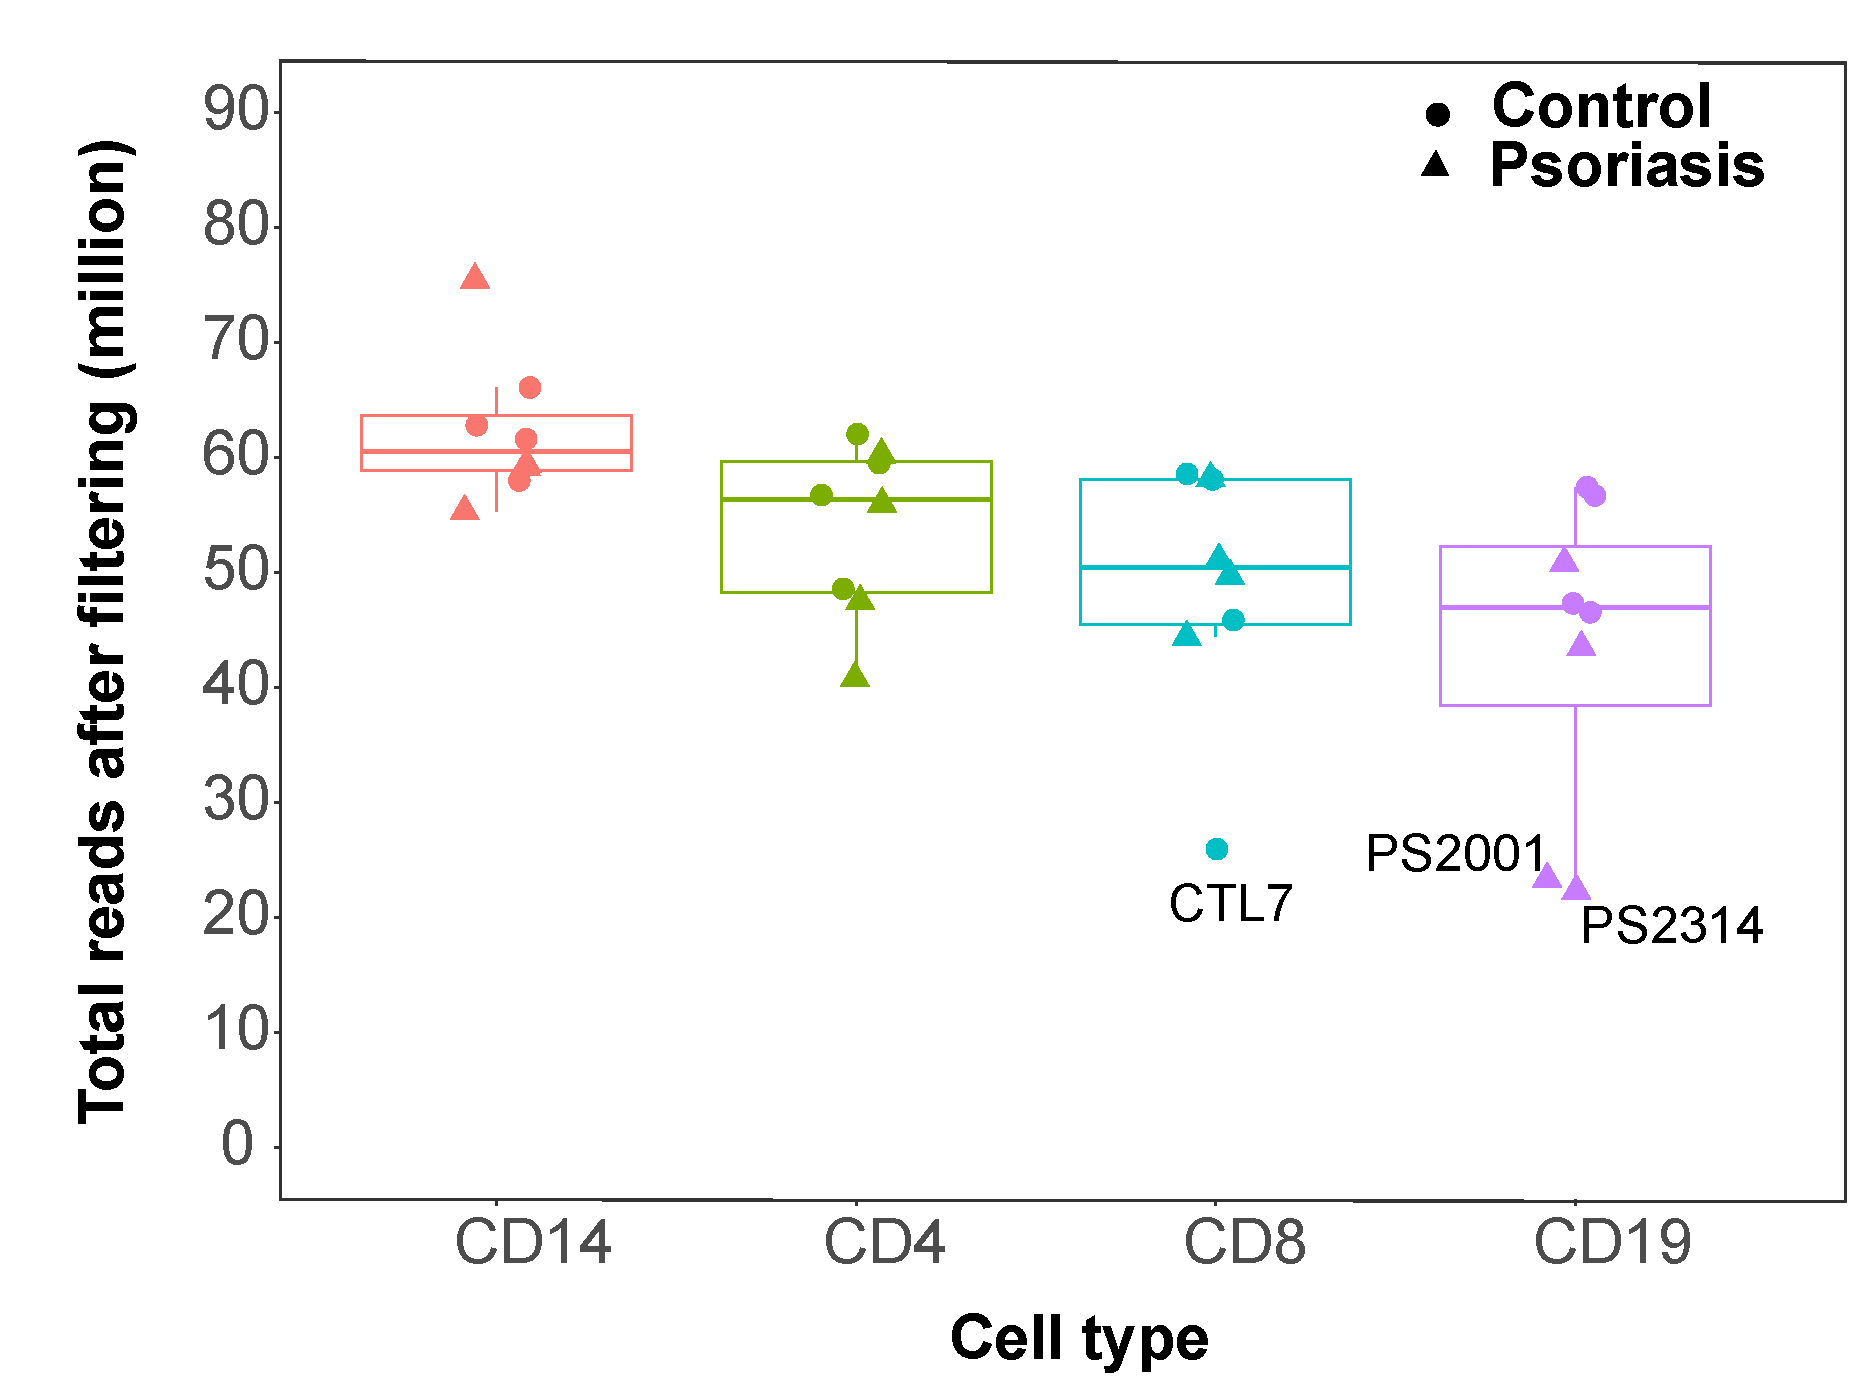
\includegraphics[width=\textwidth]{./Results2/pdfs/ChIPm_PS_CTL_final_filtered_reads_boxplot}
\caption{}
\end{subfigure}%
~
\begin{subfigure}{0.50\textwidth}
\centering
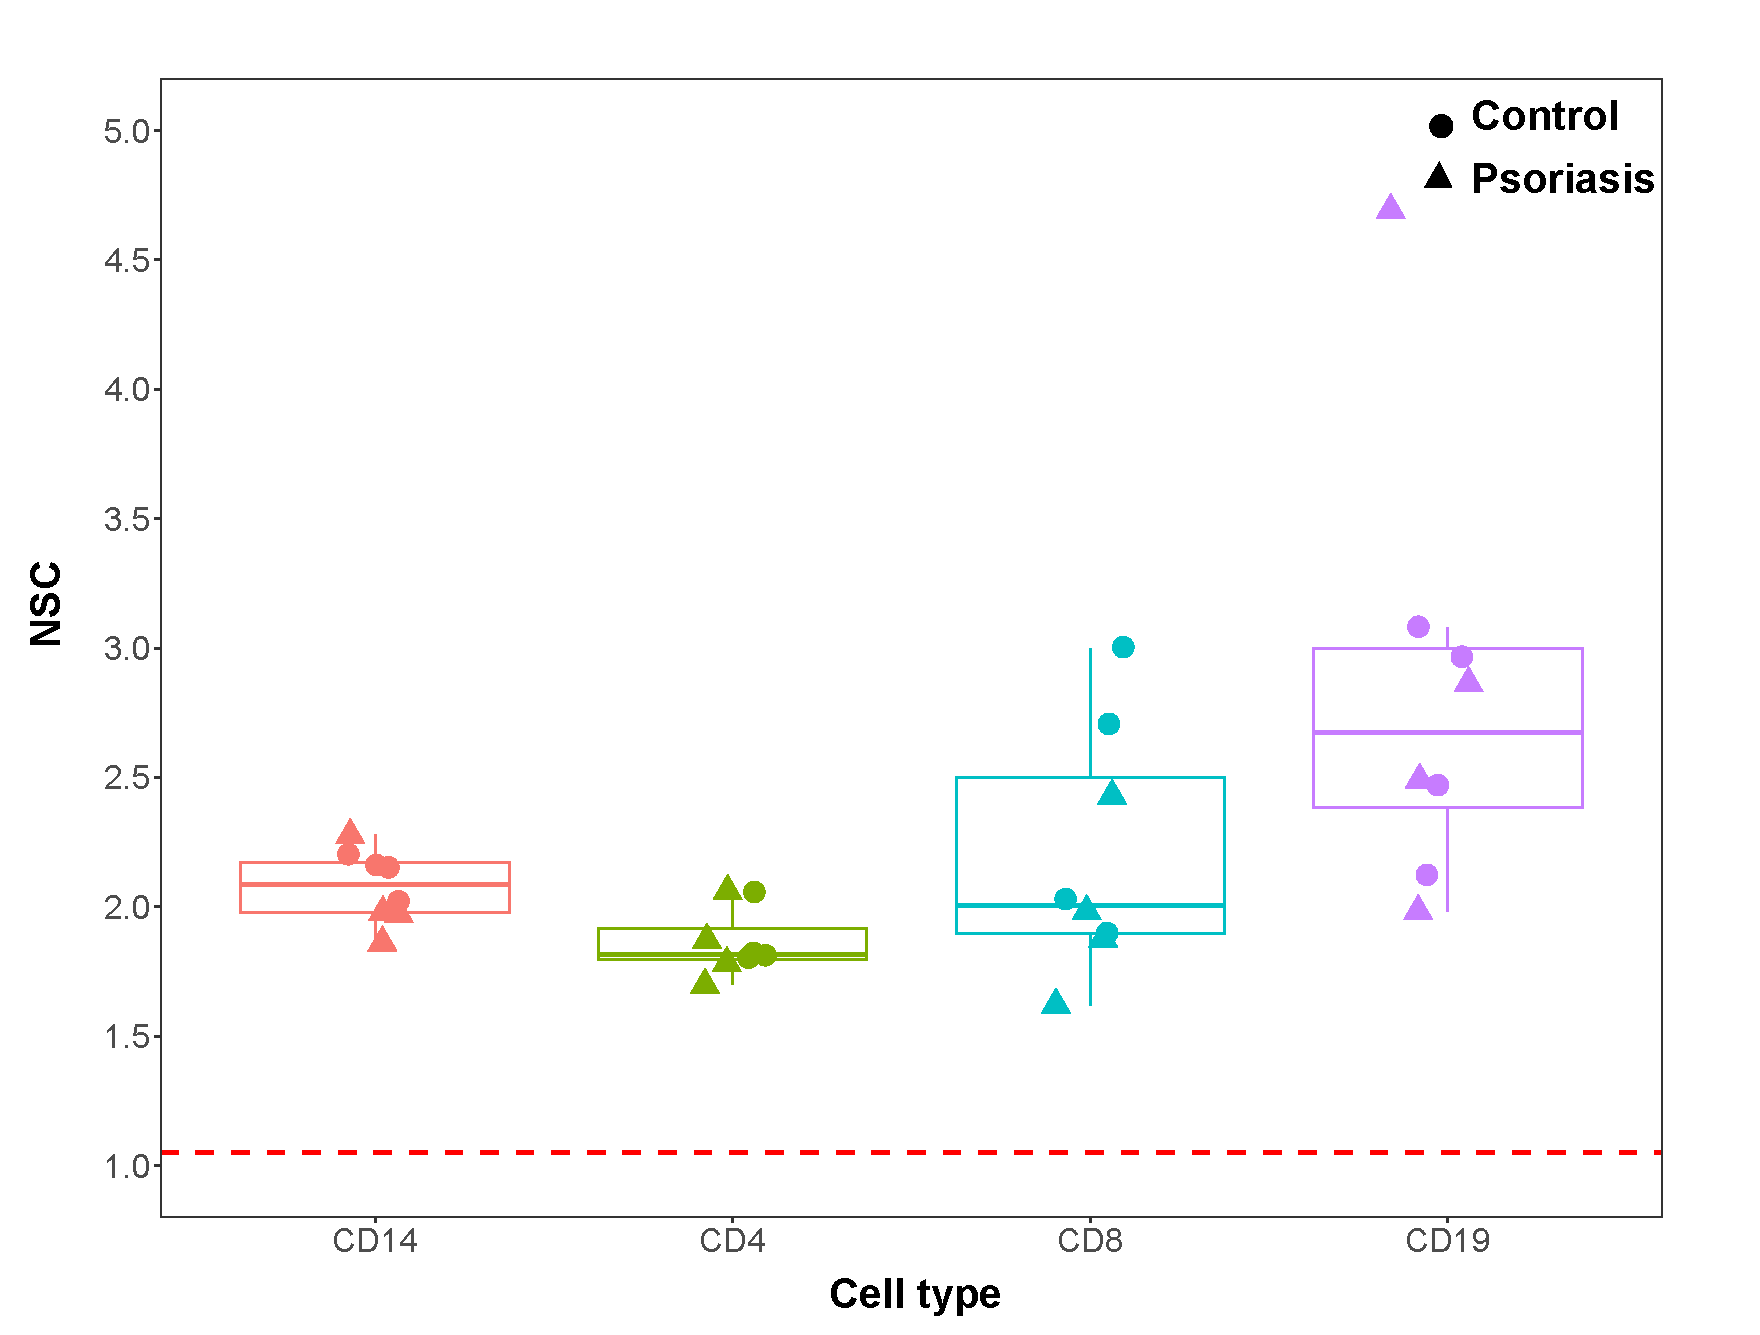
\includegraphics[width=\textwidth]{./Results2/pdfs/ChIPm_PS_CTL_NSC_boxplot}
\caption{}
\end{subfigure}
~
\begin{subfigure}{0.50\textwidth}
\centering
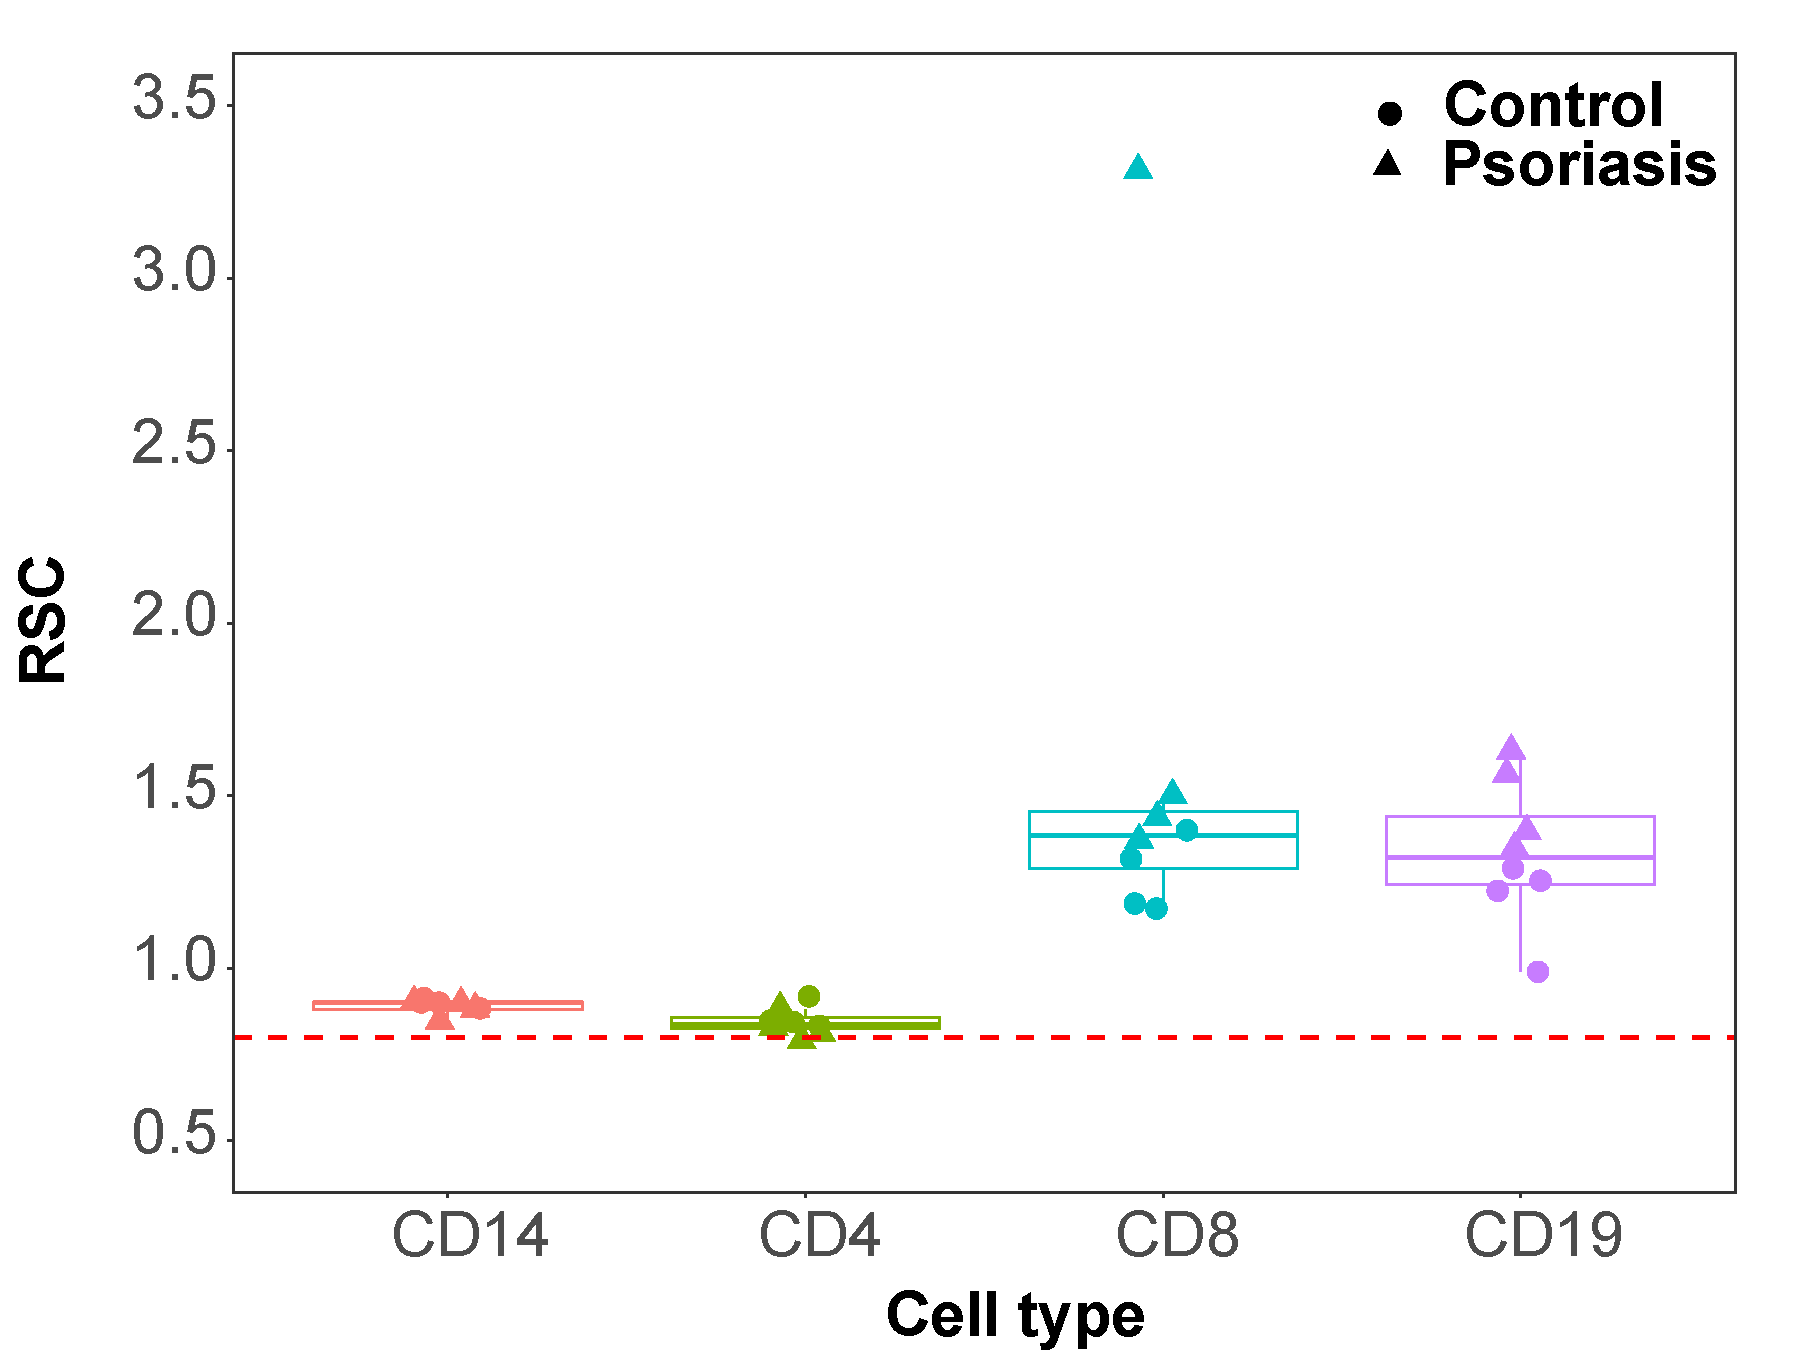
\includegraphics[width=\textwidth]{./Results2/pdfs/ChIPm_PS_CTL_RSC_boxplot}
\caption{}
\end{subfigure}
\caption[Quality control evaluation of the H3K27ac ChIPm libraries in immune cells isolated from psoriasis and control samples.]{\textbf{Quality control evaluation of the H3K27ac ChIPm libraries in immune cells isolated from psoriasis and control samples.} For each of the cell types boxplots representing (A) million of reads after filtering, (B) normalised strand cross-correlation coefficient (NSC) and (C) relative strand cross-correlation coefficient (RSC). NSC and RSC are measures of signal enrichment independent of peak calling, where 1 and 0 indicate no enrichment, respectively. In (B) and (C) the dashed red line indicates the ENCODE threshold for low enrichment (NSC$<$1.05 and RSC$<$0.8). For each point, colour codes for cell type and shape for phenotype (psoriasis or control).}
\label{figure:ChIPm_PS_CTL_QC}
\end{figure} 





\begin{figure}[htbp]
\centering
\begin{subfigure}{0.65\textwidth}
\centering
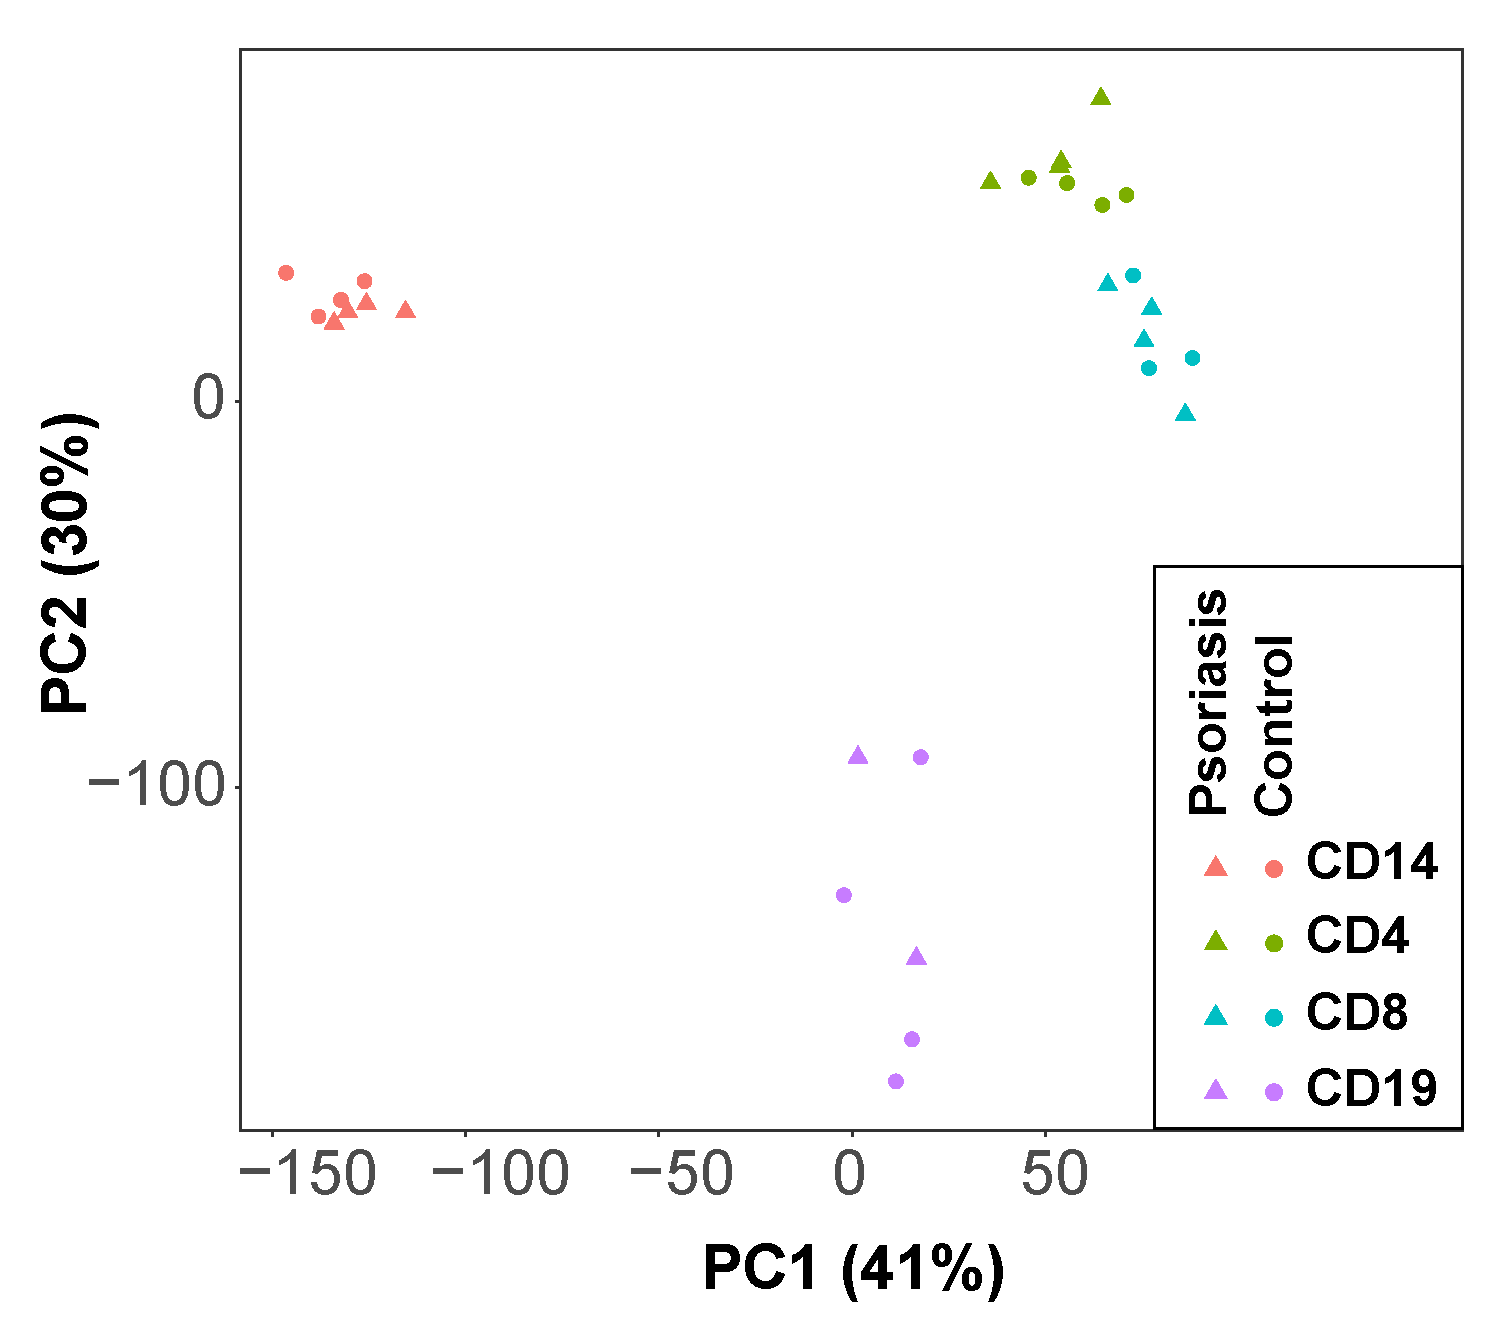
\includegraphics[width=\textwidth]{./Results2/pdfs/ChIPm_H3K27ac_all_cell_types_filtered_PCA}
\caption{\textbf{}}
% The percentage sign indicated that the other subfig goes side by side
\end{subfigure}
\begin{subfigure}{0.7\textwidth}
\centering
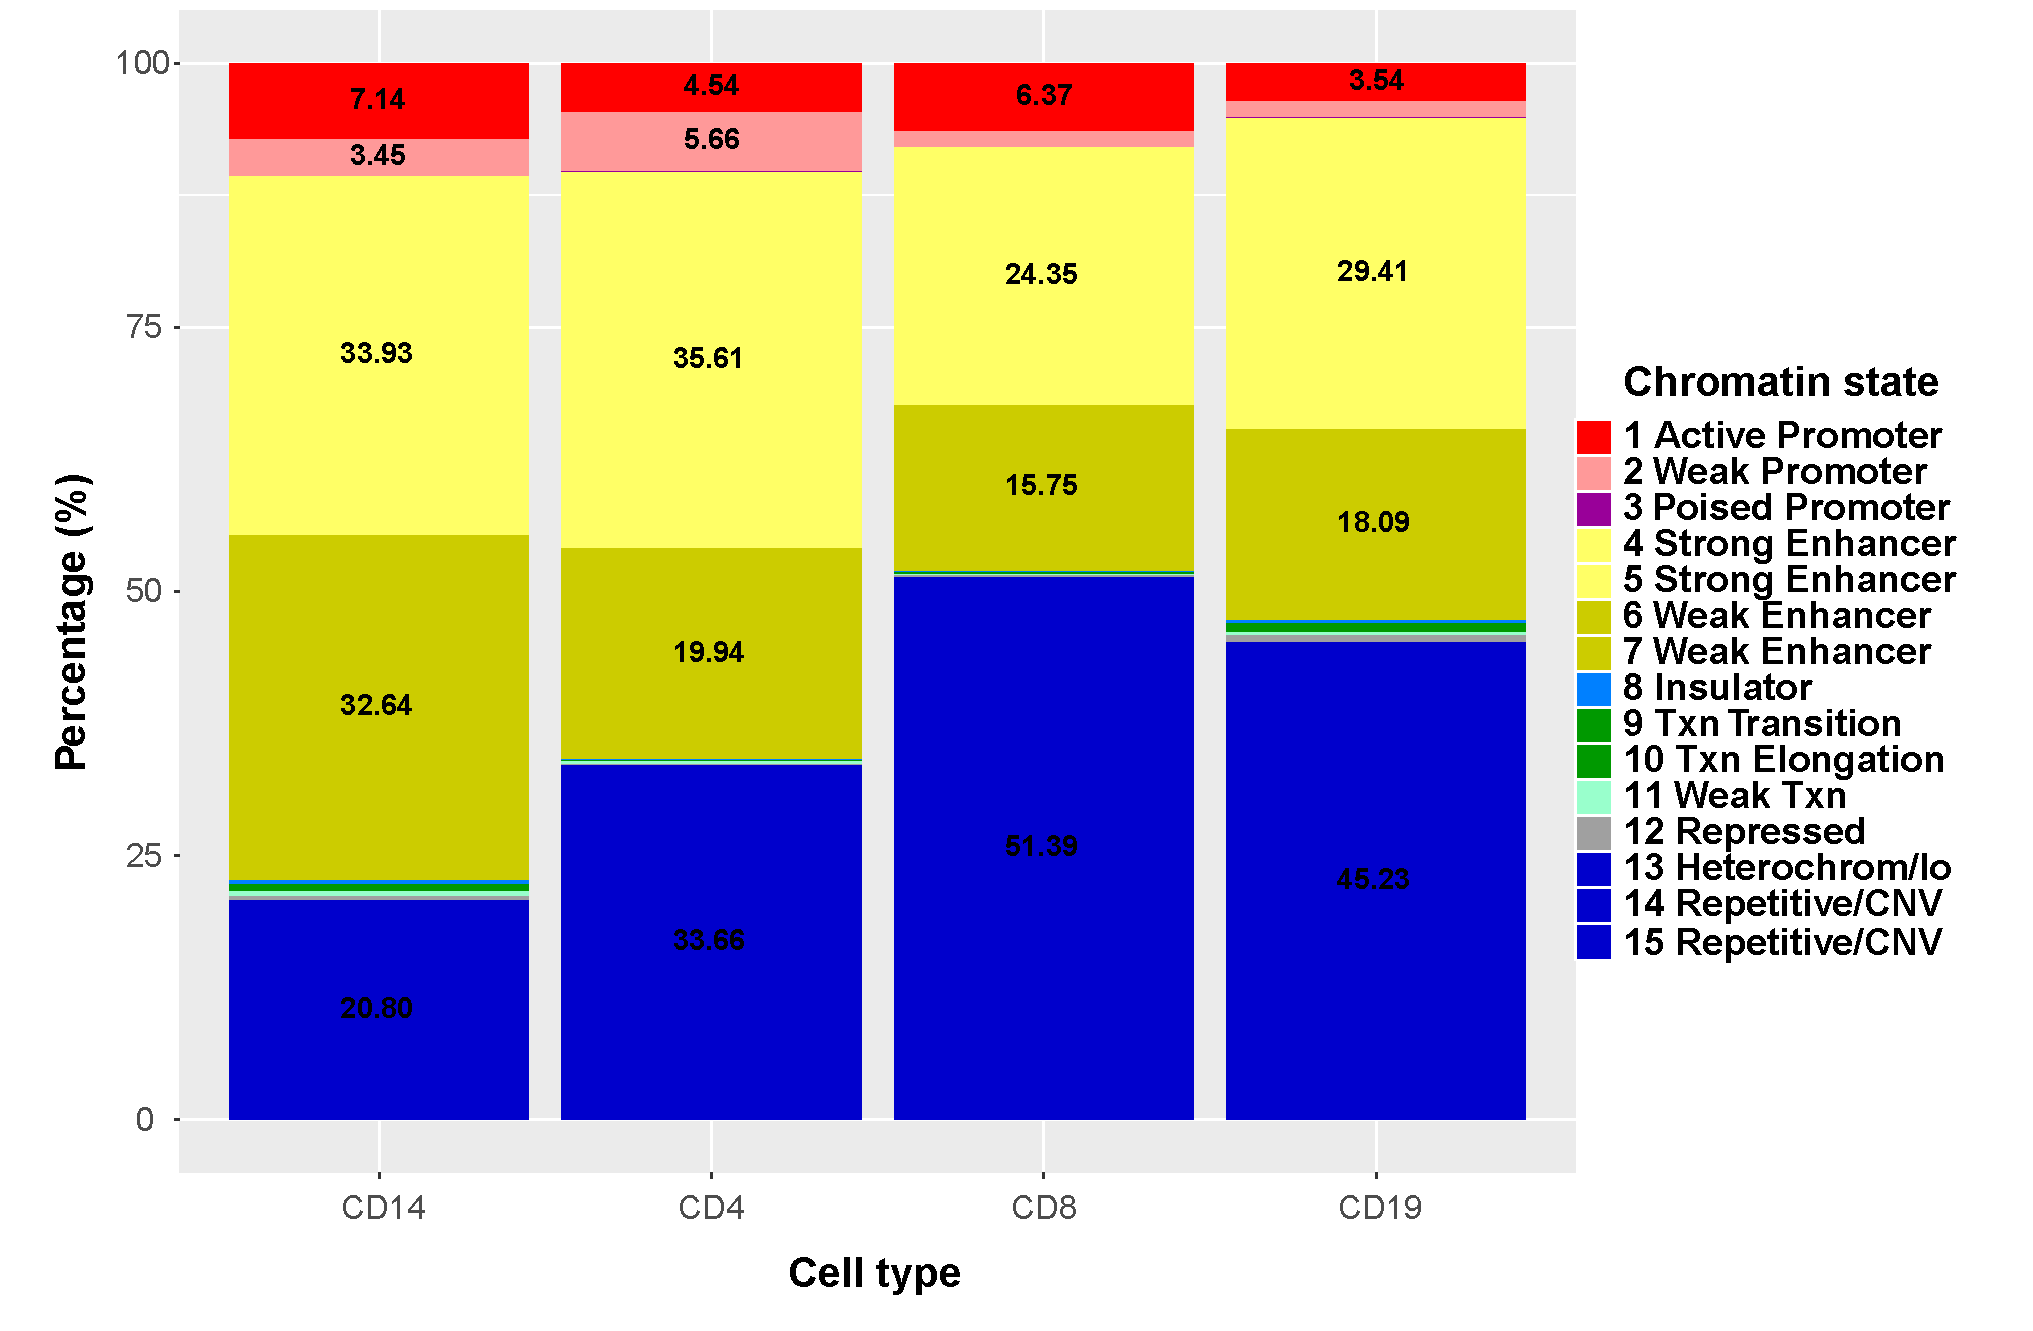
\includegraphics[width=\textwidth]{./Results2/pdfs/ChIPm_H3K27ac_cell_type_specific_master_list_chromatin_states_annotated_filtered}
\caption{\textbf{}}
\end{subfigure}
\caption[PCA and chromatin annotation states of the consensus list of H3K27ac called peaks in four immune primary cell types from psoriasis and healthy control samples.]{\textbf{PCA and chromatin annotation states of the consensus list of H3K27ac called peaks in four immune primary cell types from psoriasis and healthy control samples.} (A) PCA was performed using the normalised counts across a consensus master list of the combined H3K27ac enriched regions in psoriasis patients and healthy control samples across CD14$^+$ monocytes, CD4$^+$, CD8$^+$ and CD19$^+$ cells. %The first two PCs (x-axis and y-axis, respectively) for all the H3K27ac ChIPm peaks in the master list are plotted. 
(B) Annotation of the H3K27ac list of consensus enriched sites built by DiffBind for each cell was performed using the appropriate cell-type specific Roadmap Epigenomics Project chromatin segmentation maps. Results are expressed as the percentage of regions annotated with a particular chromatin state over the total number of H3K27ac enriched sites in each individual cell type master list.}
\label{figure:ChIPm_PCA_and_chromatin_states}
\end{figure}


\subsubsection{H3K27ac differential analysis}
An exploratory analysis was conducted to find differences in H3K27ac patterns between patients and controls using DiffBind in each cell type. DiffBind assembled a consensus list of H3K27ac peaks used to perform differential analysis (as explained in Chapter \ref{ch:Mat} and Table \ref{tab:ChIPm_DiffBind_master_list}). Annotation with chromatin states of each consensus list of H3K27ac peaks showed a high percentage of sites annotated as repressed and quiescent (Figure \ref{figure:ChIPm_PCA_and_chromatin_states}B), ranging from 20.8\% in CD14$^+$ monocytes to 51.39\% in CD8$^+$ cells. Such sites are less likely to be relevant since H3K27ac is a histone modification mainly enriched at enhancer elements. Therefore, the differential analysis for H3K27ac modifications between psoriasis and healthy control samples in each cell type was restricted to those H3K27ac peaks annotated as enhancers or transcribed (Table \ref{tab:ChIPm_DiffBind_master_list}). CD14$^+$ monocytes had the greatest number of differentially modified enhancers (8 significant sites), followed by CD4$^+$ (4) and CD8$^+$ (1) (Table \ref{tab:ChIPm_differential_analysis_results}).



\begin{table}[htbp]
%\setlength{\tabcolsep}{20pt} only to stretch the columns if you want
%\renewcommand{\arraystretch}{1.5}
\centering
\begin{tabular}{@{} c c c}
\toprule
\textbf{Cell type}   & \textbf{Differential H3K27ac}      & \textbf{Differential H3K27ac}      \\
                     & \textbf{genome-wide analysis}              & \textbf{enhancers analysis}     \\
\midrule
\midrule
CD14$^+$             & 15                 & 8                                \\
CD4$^+$              & 0                  & 4																	\\
CD8$^+$              & 8                  & 1                                 \\ 
CD19$^+$             & 12                 & 0                                 \\
\bottomrule 
\end{tabular}
\medskip %gap
\caption[Summary results from the differential H3K27ac analysis between psoriasis patients and healthy controls in CD14$^+$ monocytes, CD4$^+$, CD8$^+$ and CD19$^+$ cells.]{\textbf{Summary results from the differential H3K27ac analysis between psoriasis patients and healthy controls in CD14$^+$ monocytes, CD4$^+$, CD8$^+$ and CD19$^+$ cells.} Differential analysis was performed genome-wide in all the DiffBind H3K27ac consensus sites or only at the consensus sites annotated as enhancers (according to the chromatin segmentation map from Roadmap Epigenomics Project). Genome-wide differential significant sites in CD14$^+$ monocytes and CD8$^+$ also contain the sites identified in the enhancer restricted analysis. Significant differentially H3K27ac modified regions were determined using FDR$<$0.05 and no fold change threshold.}
\label{tab:ChIPm_differential_analysis_results}
\end{table}
\bigskip %bigger space


When comparing patients vs controls, several H3K27ac differentially modified regions were proximal to genes relevant in chronic inflammation. For example, a differential H3K27ac region in CD14$^+$ monocytes was located between the \textit{SLC15A2} and \textit{ILDR2} genes (Figure \ref{figure:ChIPm_H3K27ac_UCSC_ILDR1_track}). \textit{ILDR2} has recently been identified as relevant for negative regulation of T cell response in RA \parencite{Hecht2018}. This region showed lower H3K27ac levels in psoriasis patients compared to controls and was annotated as enhancer by the Roadmap Epigenomics Project chromatin segmentation map. Additionally this site was overlapping a DHS and H3K4me1 (enhancer mark) modification and a CTCF-binding site in K562 cells. %Publicly available chromatin conformation data in T cells failed to show interactions of this region with the promoter of any of the proximal genes in monocytes and eQTL data has suggested regulation of the calmodulin-binding motif-containing protein \textit{IQCB1} gene in monocytes and CD4$^+$ cells \parencite{GTeX,Fairfax2014, Kasela2017}. Amongst the CD4$^+$ hits, all the significant regions presented minor changes with no evidence of regulating expression of any relevant gene by proximity or based on chromatin conformation data. 


%Conversely, this region harbours SNPs that have been identified as \textit{cis}-eQTL in whole blood and total unstimulated and stimulated CD14$^+$ monocytes for the calmodulin-binding motif-containing protein \textit{IQCB1} gene, which is 186.4Kb up-stream of this peak \parencite{GTeX,Fairfax2014}. MS risk LD SNPs (rs34543553, rs73855480 and rs73855480) in this peak are also \textit{cis}-eQTLs in unstimulated total CD4$^+$ and CD8$^+$ cells for \textit{IQCB1} \parencite{Kasela2017}. 



\begin{figure}[ht]
\centering
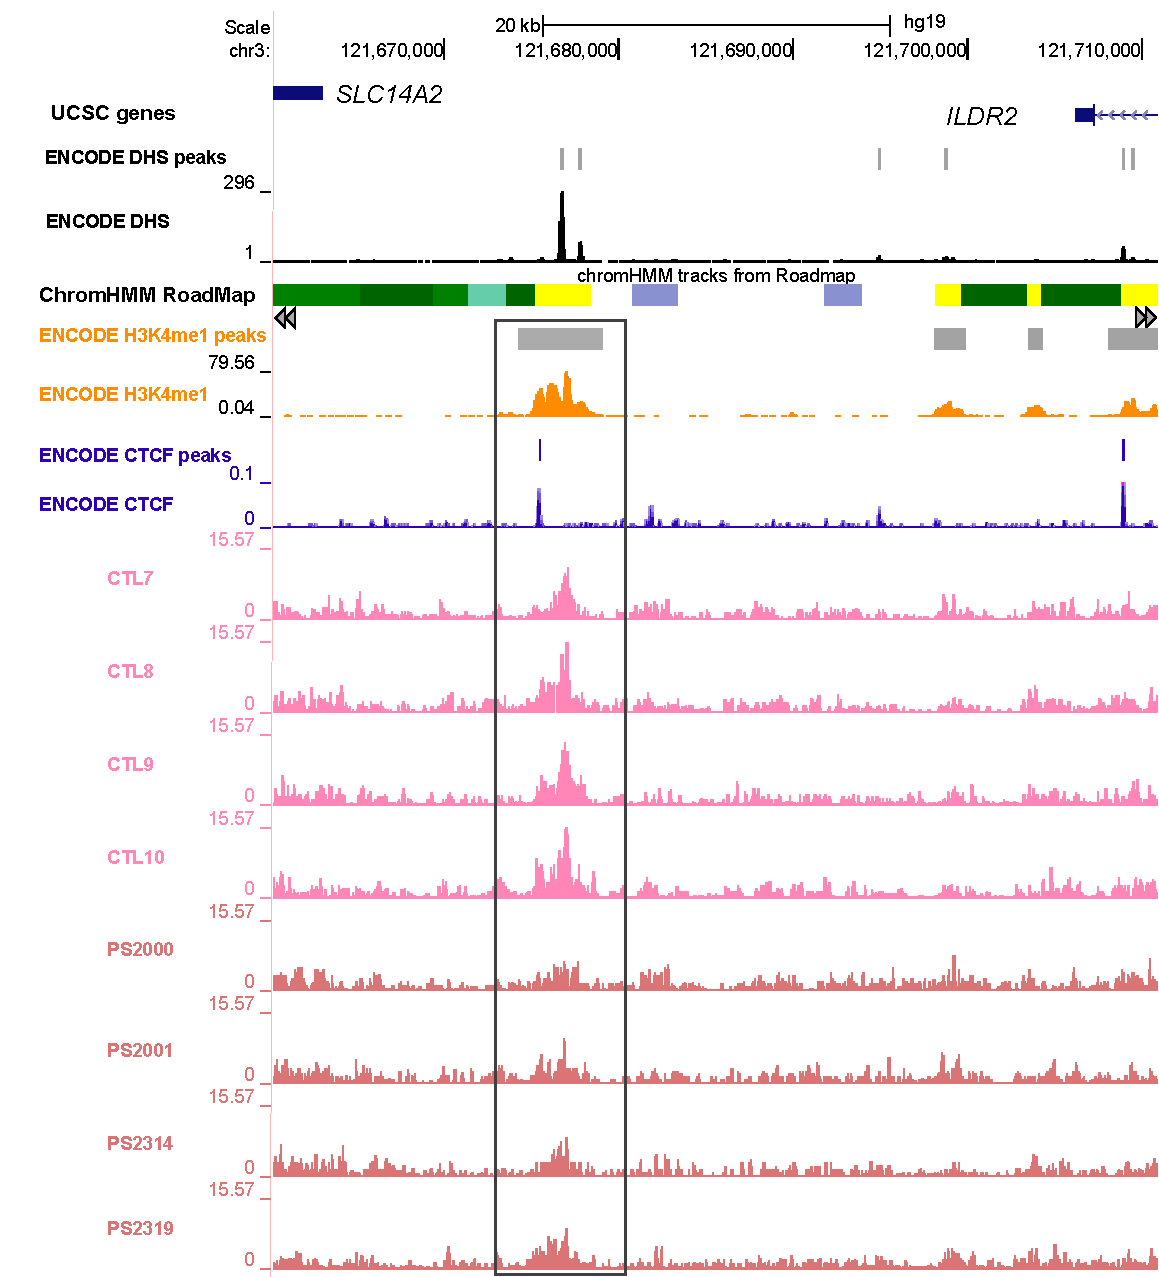
\includegraphics[width=0.6\textwidth]{./Results2/pdfs/ChIPm_H3K27ac_UCSC_CD14_ILDR1_track}
\caption[Differential H3K27ac modification at a putative intergenic enhancer region in circulating CD14$^+$ monocytes between psoriasis patients and healthy controls.]{\textbf{Differential H3K27ac modification at a putative intergenic enhancer region in circulating CD14$^+$ monocytes between psoriasis patients and healthy controls.} UCSC Genome Browser view illustrating the normalised H3K27ac fold-enrichment (y-axis) at an intergenic differentially modified region located between \textit{SLC14A2} and \textit{ILDR2} genes (x-axis) in CD14$^+$ monocytes (lower H3K27ac enrichment in psoriasis patients compared to healthy controls). CD14$^+$ monocytes publicly available epigenetic data from ENCODE (including DHS, H3K4me1 and CTCF ChIP-seq) and the Roadmap Epigenomics Project chromatin segmentation track are also shown. Differential H3K27ac modified regions were considered significant based on FDR$<$0.05 and no fold change cut-off. H3K27ac tracks are colour-coded by condition: control(CTL)=pink and psoriasis (PS)=sienna.}
\label{figure:ChIPm_H3K27ac_UCSC_ILDR1_track}
\end{figure}



In addition to the restricted analysis at enhancers and transcribed regions, genome-wide contrast between psoriasis and control samples revealed additional H3K27ac differential regions in CD14$^+$ monocytes and CD8$^+$ cells, which also included those already identified in the restricted enhancer analysis (Table \ref{tab:ChIPm_differential_analysis_results}). Comparison of both approaches revealed that restricting the analysis to enhancer and transcribed annotated regions based on chromatin segmentation maps did not significantly increase the number of observed differentially modified H3K27ac sites when compared to the genome-wide analysis in any of the four cell types. Altogether, the results presented in this pilot cohort did not show relevant global epigenetic changes in H3K27ac sites between psoriasis patients and controls for these cell types and sample size.
%The newly identified regions in both cell types were mostly in regions lacking DHS and  H3K4me1 modifications. Genome-wide analysis in CD4$^+$ cells did not reveal significant differentially modified targets outside enhancers and also failed to retain significance for the four hits identified in the restricted analysis, most likely due to increase in multiple testing as a result of the larger size of the master list (Table \ref{tab:ChIPm_DiffBind_master_list}). The differential regions between psoriasis patients and controls identified in CD19$^+$ cells when performing genome-wide analysis presented considerable fold changes (absolute log$_2$fold change ranging from 2.47 to 6.37). However, most of them (10 out of 12) did not overlap accessible chromatin and none were found to be interacting with other enhancers or distal promoters. The  absence of differentially H3K27ac sites between patients and controls at CD19$^+$ enhancers may reinforce the limited relevance for B cells in psoriasis when compared to the other three cell types.




\subsection{Interrogation of chromatin accessibility changes in  psoriasis peripheral blood immune cells}

%The cell type specific chromatin accessibility landscape is determined by the combination of histone modifications and DNA binding proteins (including TF and co-regulatory proteins) in a particular locus. The previous results showing only moderate changes in the H3K27ac landscape between patients and controls are not necessarily representative of the overall changes in the chromatin accessibility landscape in disease. 
In order to interrogate genome-wide changes in chromatin accessibility between psoriasis patients and healthy controls, ATAC (ATAC-seq or Fast-ATAC) was performed in the same four cell types in eight patients and ten controls (Tables \ref{tab:Psoriasis_cohort_metadata} and \ref{tab:Control_cohort_metadata}) yielding a total of 72 libraries.


\subsubsection{Data processing and quality control}
The median total reads after filtering for all the ATAC libraries ranged between 39.2 and 49.8 million, above the 15 million reads determined as the minimum depth for downstream analysis (detailed in Chapter \ref{ch:Results1}) (Figure \ref{figure:ATAC_PS_CTL_QC}A). All samples showed the required characteristic ATAC-seq fragment size distribution recapitulating nucleosome periodicity (not shown) and differences in the percentage of mitochondrial reads between ATAC-seq and Fast-ATAC libraries were also found (detailed in \ref{ch:Results1} and Figure \ref{figure:ATAC_PS_CTL_MT_percent_and_called_peaks}A). Analysis of ATAC signal enrichment across gene TSSs revealed that most samples had enrichment over 6 (Figure \ref{figure:ATAC_PS_CTL_QC}B). CD14$^+$ PS2000 and PS2001 monocytes showed TSS$<$6 and were removed from downstream analysis together with CD19$^+$ CTL2, which TSS was borderline.  %For example, CD14$^+$ monocytes had greater numbers of peaks when compared to the other three cell types, despite the median total number of reads after filtering being similar to the other cell types (Figure \ref{figure:ATAC_PS_CTL_QC}A). %Also, within the CD14$^+$ monocytes samples, those with the greatest TSS fold-enrichment (e.g CTL4, CTL6 and PS2314) presented similar numbers of good quality called peaks to the samples with higher numbers of reads after filtering and lower signal-to-noise ratios (e.g  PS1011, CTL1 and CTL3) (Figure \ref{figure:ATAC_PS_CTL_QC} a and c).

Regarding the number of called peaks, most samples showed between 10,000 and 35,000 peaks after IDR filtering (Figure \ref{figure:ATAC_PS_CTL_MT_percent_and_called_peaks}B) and the majority of differences in numbers were intrinsic to cell type and signal-to-noise variability across libraries (Figure \ref{figure:ATAC_PS_CTL_QC}C). For example, CD19$^+$ CTL2 showed lower number of filtered peaks compared to other samples with similar sequencing depth but larger signal-to-noise enrichment, supporting removal of this sample from downstream analysis.


\begin{figure}[htbp]
\centering
\begin{subfigure}{0.55\textwidth}
\centering
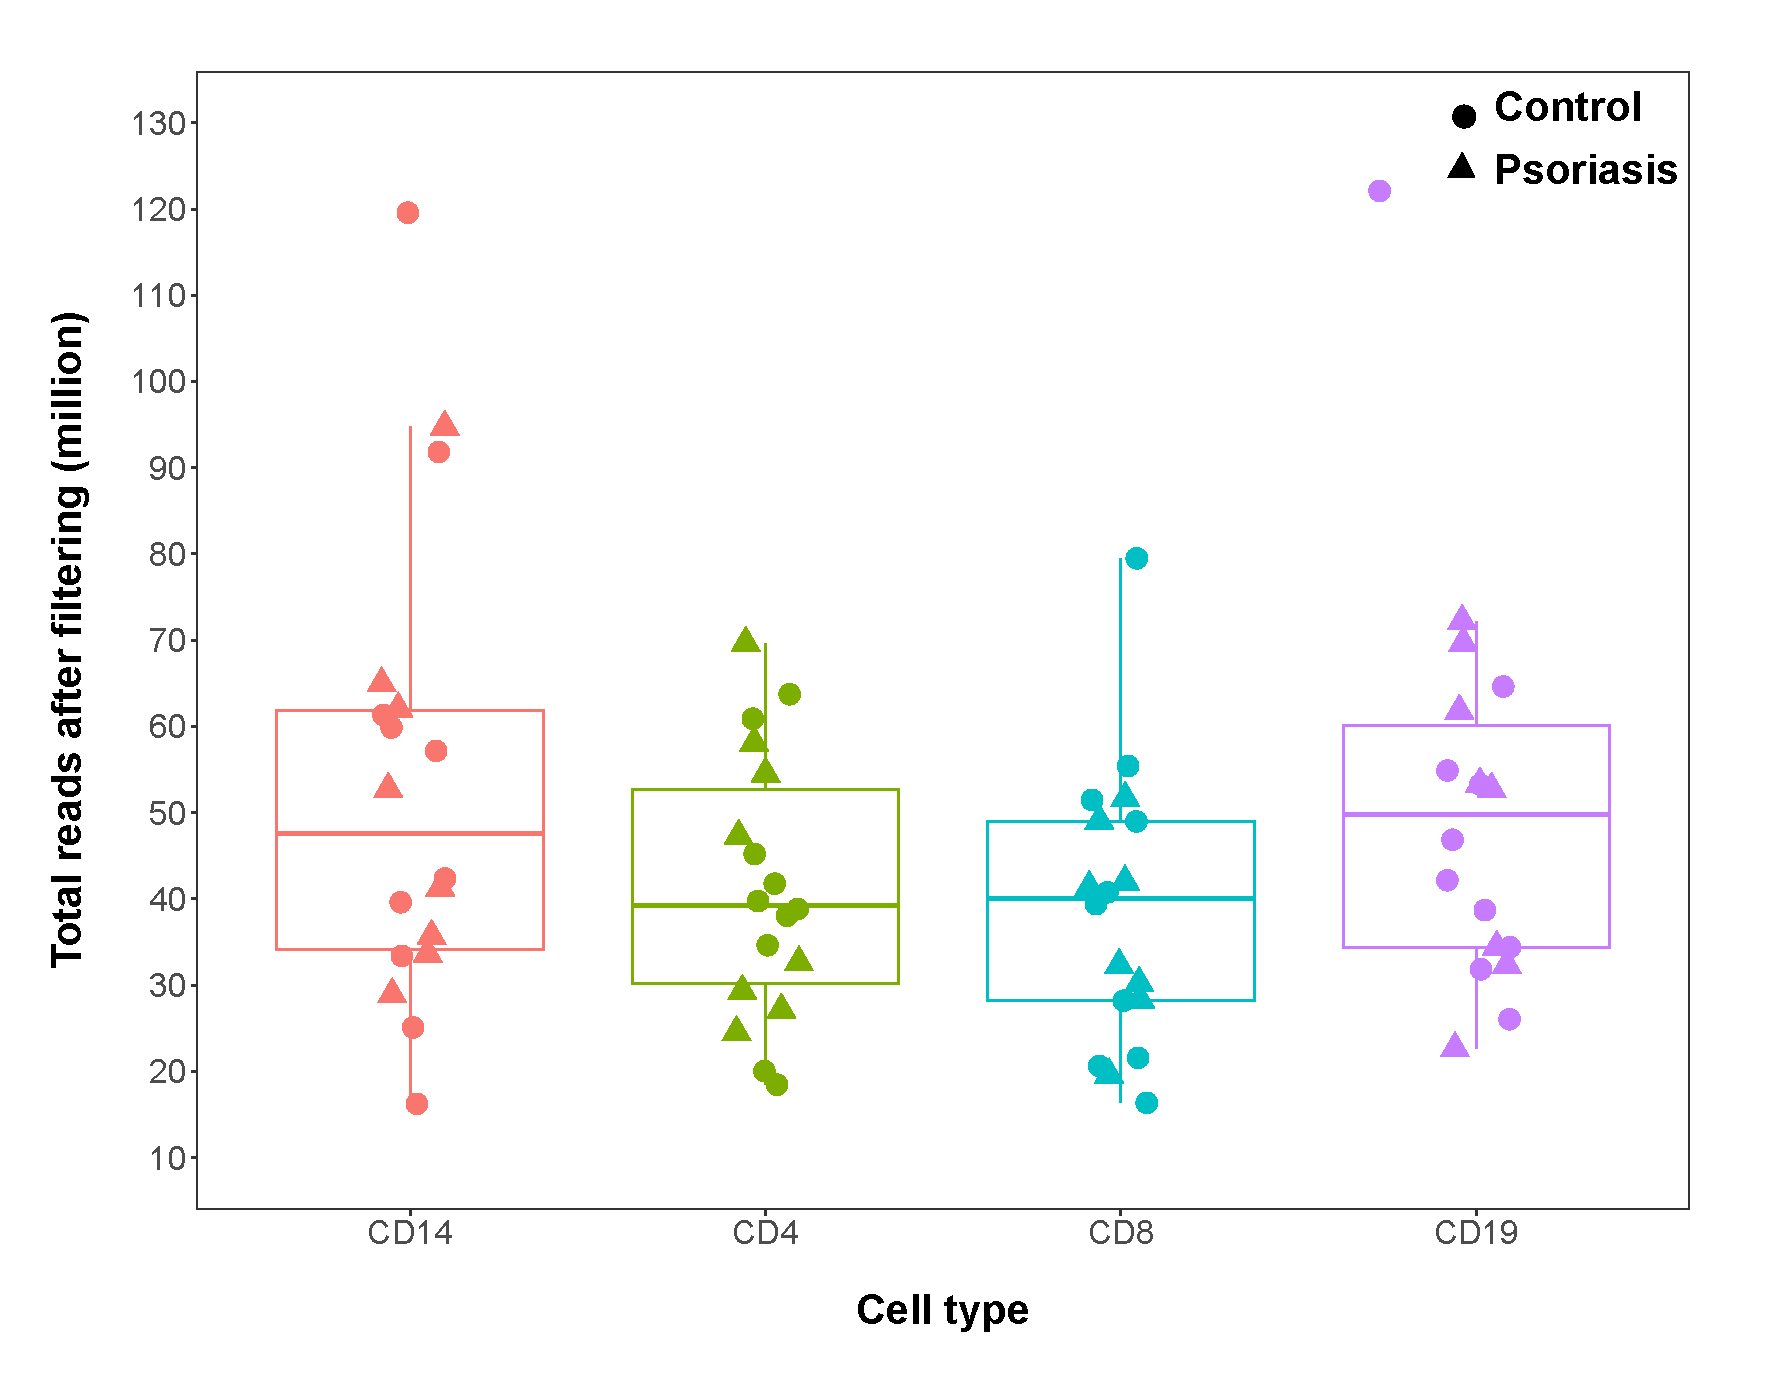
\includegraphics[width=\textwidth]{./Results2/pdfs/ATAC_PS_CTL_final_filtered_reads_boxplot}
\caption{\textbf{}}
% The percentage sign indicated that the other subfig goes side by side
\end{subfigure}
\begin{subfigure}{0.55\textwidth}
\centering
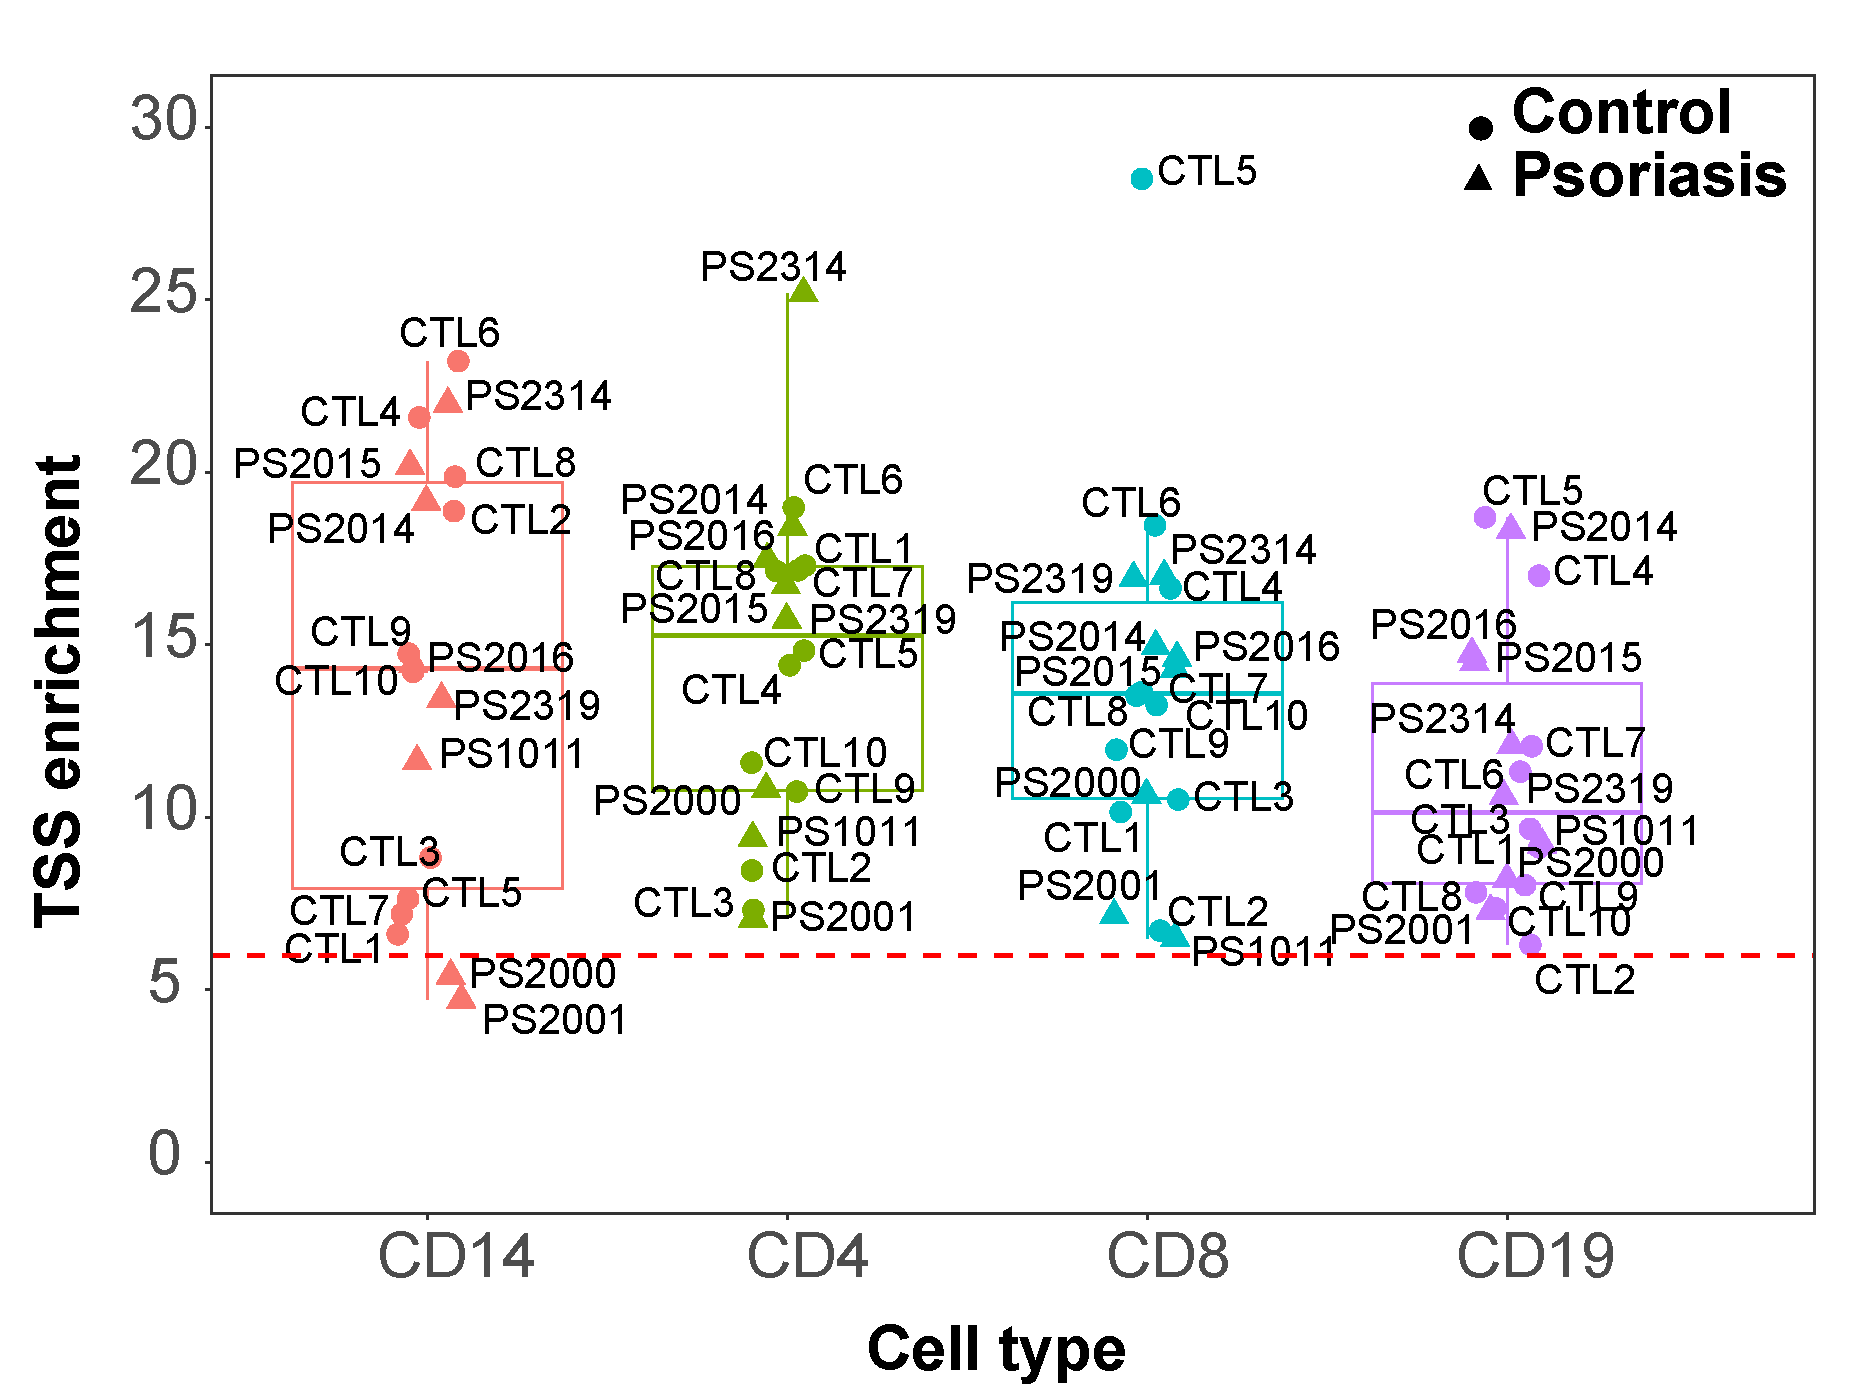
\includegraphics[width=\textwidth]{./Results2/pdfs/ATAC_PS_CTL_all_samples_TSS_boxplots_all_labelled}
\caption{\textbf{}}
\end{subfigure}
\caption[Quality control assessment of the ATAC libraries generated from circulating immune cells in psoriasis and control samples.]{\textbf{Quality control assessment of the ATAC libraries generated from circulating immune cells in psoriasis and control samples.} For each of the cell types and samples, boxplots showing (A) million of reads after filtering and (B) values for fold-enrichment of ATAC fragments across the Ensembl annotated TSS. In (B) the dashed red line indicates the recommended ENCODE threshold for TSS enrichment values. For each point, colour codes for cell type and shape for phenotype (psoriasis or control). In (B) sample IDs are included.}
\label{figure:ATAC_PS_CTL_QC}
\end{figure} 



\bigskip
\begin{figure}[htbp]
\centering
\begin{subfigure}[b]{0.7\textwidth}
\centering 
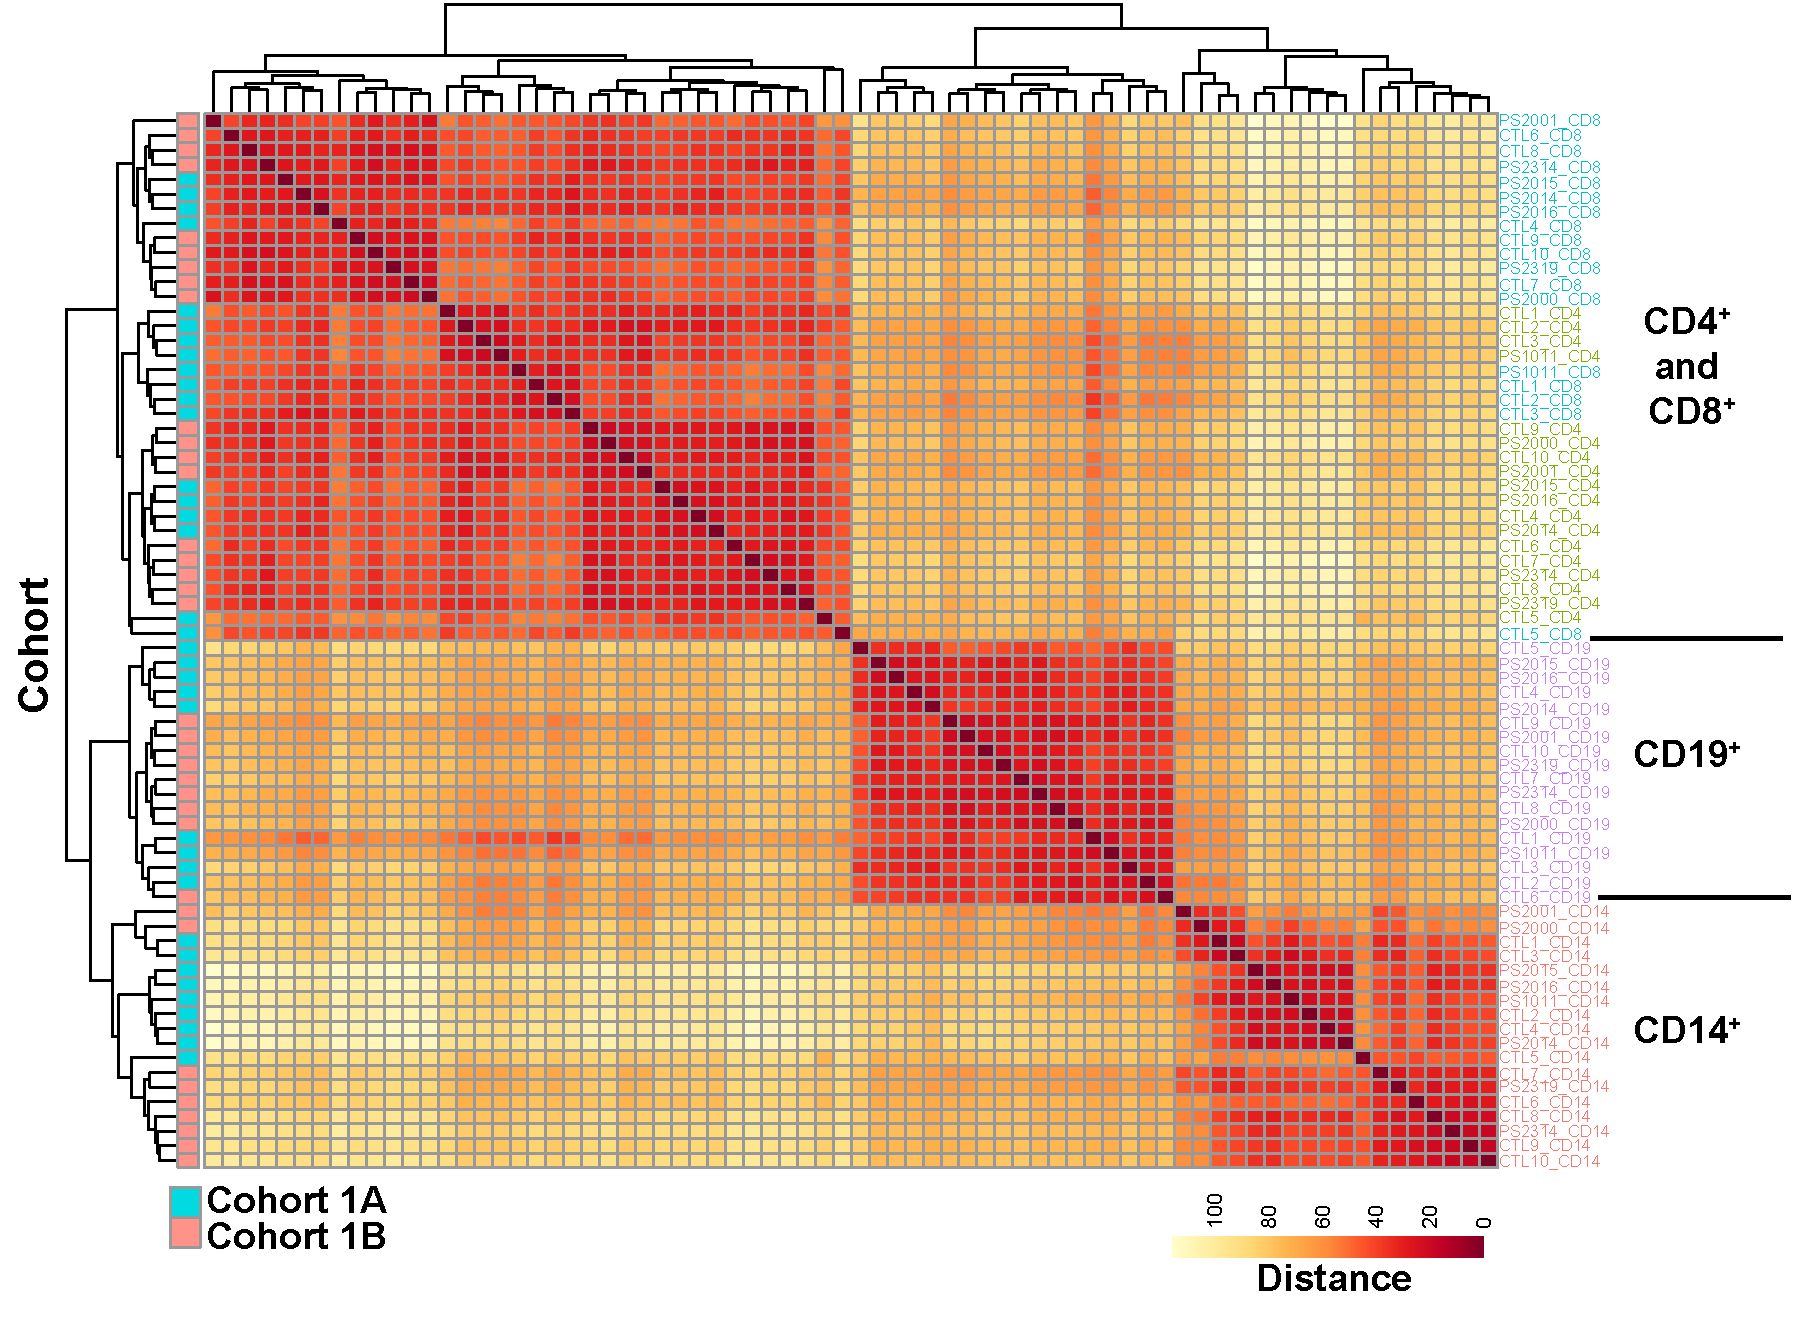
\includegraphics[width=\textwidth]{./Results2/pdfs/ATAC_all_cell_types_heatmap_with_batch_annotation}
\caption{}
\end{subfigure}
~
\begin{subfigure}[b]{0.7\textwidth} 
%the [b] prevents offset in subcaptions
\centering
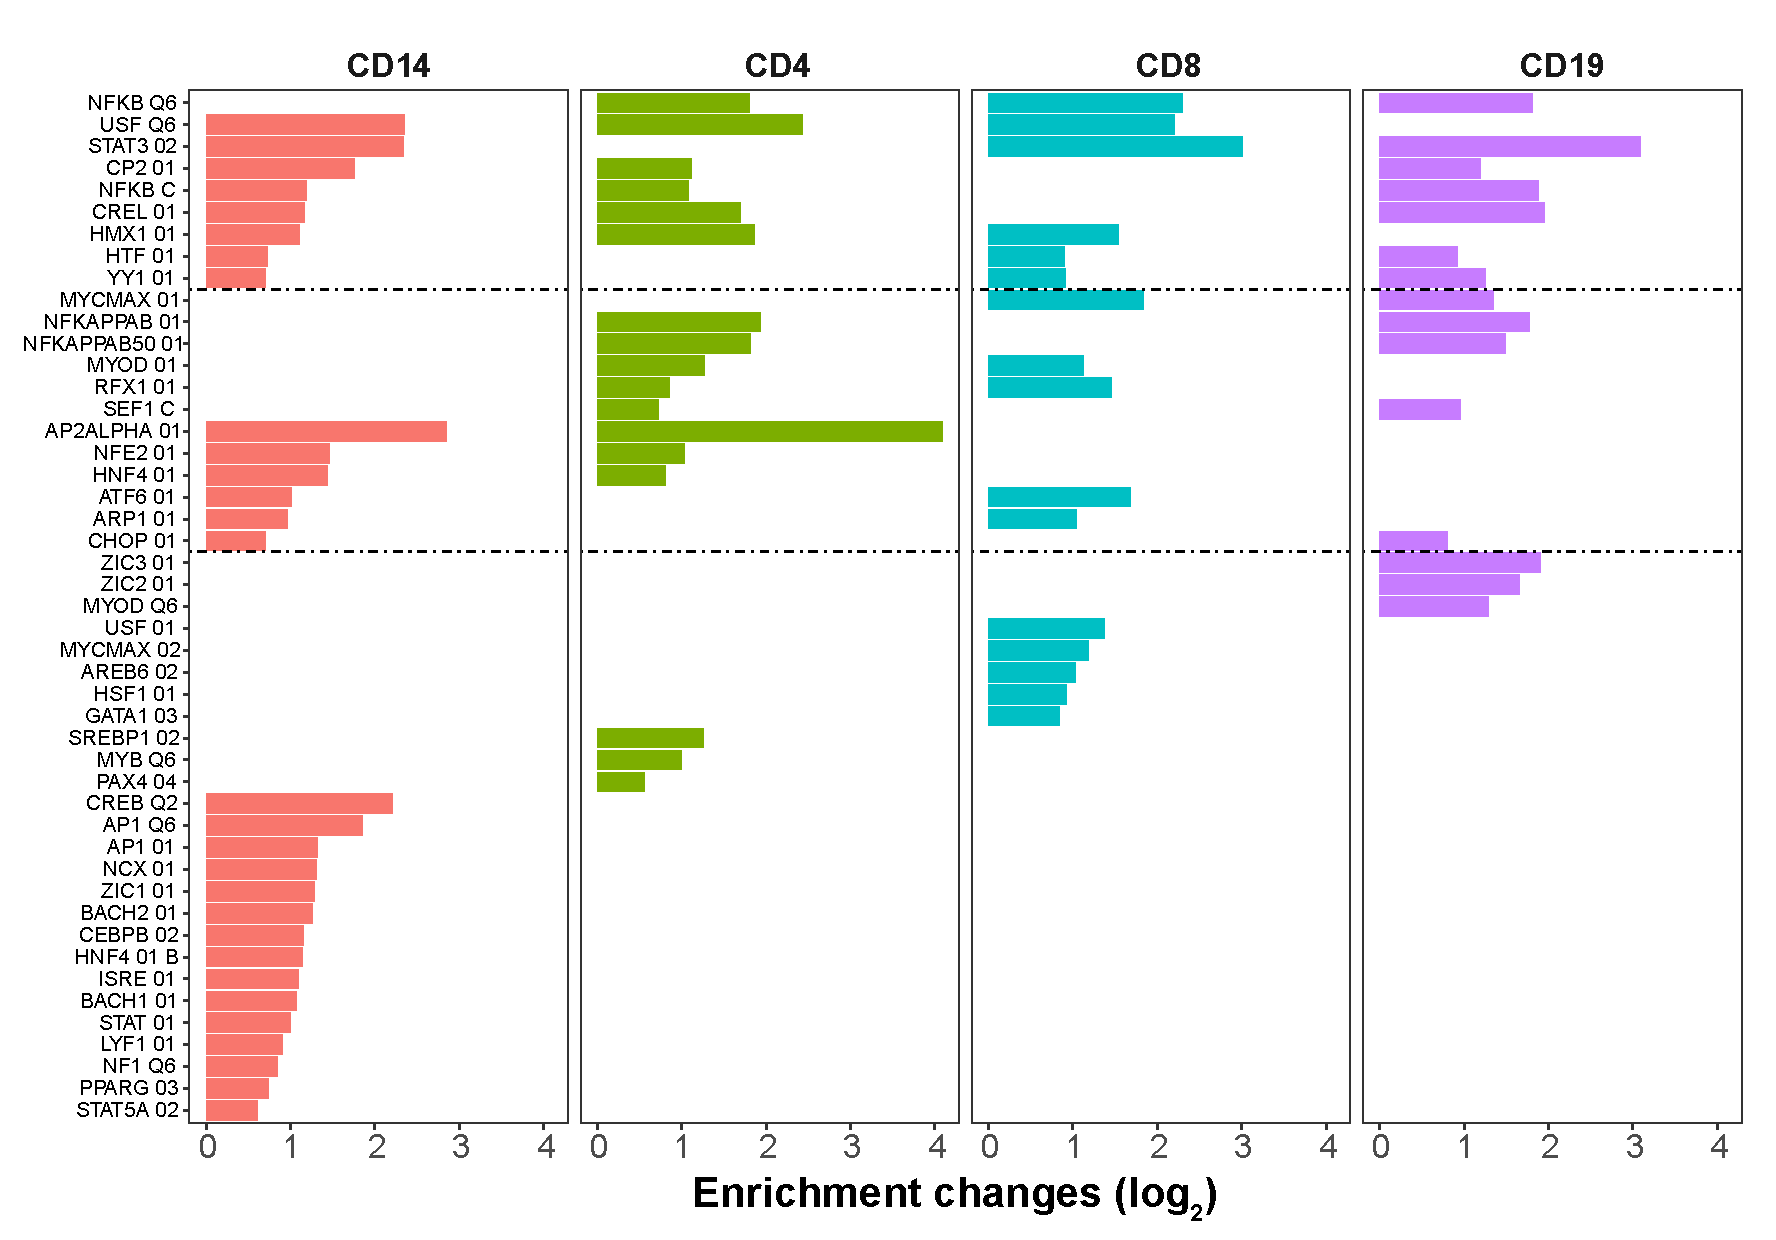
\includegraphics[width=\textwidth]{./Results2/pdfs/ATAC_PS_CTL_cell_type_specific_master_list_conserved_TFBS_enrichment}
\caption{}
\end{subfigure}
\caption[Clustered heatmap and conserved TF binding sites enrichment analysis in the consensus list of called ATAC peaks in CD14$^+$ monocytes, CD4$^+$, CD8$^+$ and CD19$^+$ cells from the patients and controls cohort.]{\textbf{Clustered heatmap and conserved TF binding sites enrichment analysis in the consensus list of called ATAC peaks in CD14$^+$ monocytes, CD4$^+$, CD8$^+$ and CD19$^+$ cells from the patients and controls cohort.} (A) Distance matrix and hierarchical clustering for the 72 samples was performed based on the normalised read counts retrieved for each sample at the regions included in a combined consensus list of called ATAC peaks across all 4 cell types (CP\_all). Clusters have been additionally annotated using cohort identity. (B) Enrichment analysis for the conserved TF binding sites was performed for each of the consensus list of ATAC peaks per cell type used for downstream differential analysis between psoriasis and control individuals (named here as CP\_CD14, CP\_CD4, CP\_CD8, and CP\_CD19). Enrichment was tested for 258 human conserved TF binding sites identified by Transfac using position-weight matrices based on experimental results in the scientific literature. Significant enrichment using FDR$<$0.01.}
\label{figure:ATAC_PS_CTL_heatmap_TFBS}
\end{figure}

A heatmap illustrating sample distance using the combined consensus list of called ATAC peaks across all the samples (named here as CP\_all) showed successful separation of the samples according to cell type into three main clusters corresponding to CD14$^+$ monocytes, CD19$^+$ and CD4$^+$/CD8$^+$ T cells (Figure \ref{figure:ATAC_PS_CTL_heatmap_TFBS}A). Within each cell type cluster, samples did not separate based on disease condition, suggesting an absence of major global differences in the chromatin accessibility landscape between psoriasis patients and healthy controls, but some grouping by batch was observed (Figure \ref{figure:ATAC_PS_CTL_heatmap_TFBS}A).

PCA per individual cell type confirmed bacth effect between cohort 1A and cohort 1B ATAC samples, likely driven by the use of ATAC-seq and Fast-ATAC protocols in each batch, respectively (representative example in CD8$^+$ cells Figure \ref{figure:ATAC_RNAseq_batch_effect}A). This analysis also revealed CTL5 as an outlier sample in cohort 1A for all the cell types and was also removed from the differential analysis.


%Each of the four cell type master lists of ATAC-seq peaks (ML\_CD14, ML\_CD4, ML\_CD8, and ML\_CD19) used for the downstream differential chromatin accessibility analysis (explained in Chapter \ref{ch:Mat}), presented the highest percentage of regions annotated as gene promoters, intronic and intergenic, as expected for ATAC-seq (Figure \ref{figure:ATAC_PS_CTL_genomic_annotation}). \textit{cis}-eQTL SNPs from a number of immune cell types, including CD14$^+$ monocytes (unstimulated and stimulated), B cells, neutrophils, CD4$^+$ and CD8$^+$ cells \parencite{Fairfax2012, Fairfax2014, Kasela2016}, were enriched within the ATAC consensus peak list of each cell type. For example, eQTLs from unstimulated and stimulated (LPS or IFN-$\gamma$) monocytes were the most significantly enriched (FDR$<$0.01) in the ML\_CD14 (unstimulated fold-enrichment 5.1, LPS 2h fold-enrichment 4.7 and IFN-$\gamma$ fold-enrichment 5.0) when compared to the other eQTL datasets. Similarly, \textit{cis}-eQTLs from CD4$^+$ and CD8$^+$ were the most enriched datasets (fold-change 8.3 and 8, respectively) in the ML\_CD8. 

%Each of the four cell type master lists of ATAC-seq peaks (ML\_CD14, ML\_CD4, ML\_CD8, and ML\_CD19) used for the downstream differential chromatin accessibility analysis (explained in Chapter \ref{ch:Mat})The specificity and functional relevance of each cell type master list was further reinforced by the significant enrichment (FDR$<$0.01) of conserved TFBS within those ATAC-seq regions (Figure \ref{figure:ATAC_PS_CTL_heatmap_TFBS} b). For example, enrichment of conserved NF$\kappa$B binding motifs was identified across each cell type list consensus ATAC peaks . Conserved binding motifs for TF involved in T cell biology, such as AREB6 (ZEB1), ATF6 and the heat-shock transcription factor HSF1 \parencite{Guan2018,Yamazaki2009,Gandhapudi2013}, were enriched in the ML\_CD8. 
%For example, enrichment of conserved binding motifs for AREB6 (ZEB1) involved in CD8$^+$ T effector and memory cell fate \parencite{Guan2018}, ATF6 implicated in NF$\kappa$B activation \parencite{Yamazaki2009} and the heat-shock transcription factor HSF1 regulator of T cell division under different types of stress \parencite{Gandhapudi2013} was found in the ML-CD8. 
%Overall, the enrichment of eQTL SNPs and conserved TFBS highlighted the potential of each cell type master list to harbour functional relevant differences in chromatin accessibility between psoriasis patients and controls.



\subsubsection{Differential chromatin accessibility analysis}

To perform differential chromatin accessibility analysis between patients and controls, a consensus list of called ATAC peaks (accessible chromatin regions) was built for each of the four cell types (named here as CP\_CD14, CP\_CD4, CP\_CD8, and CP\_CD19) (detailed in Chapter \ref{ch:Mat}). To determine the functional relevance of this consensus list of peaks used in the downstream comparison between patients and controls, enrichment analysis for conserved TF binding sites was conducted. All four cell types consensus list of peaks (CP) showed significant enrichment (FDR$<$0.01) for a number of TF binding sites (Figure \ref{figure:ATAC_PS_CTL_heatmap_TFBS}B). For example, enrichment for conserved NF$\kappa$B binding motifs was identified across the four cell types consensus list of ATAC peaks. Conserved binding motifs for TF involved in T cell biology, such as AREB6 (ZEB1), ATF6 and heat-shock transcription factor HSF1 were enriched in the CP\_CD8 \parencite{Guan2018,Yamazaki2009,Gandhapudi2013}. Additionally, peaks from each cell type consensus list also showed enrichment for relevant cell type \textit{cis}-eQTLs. For example, eQTLs from unstimulated monocytes were significantly enriched (FDR$<$0.01) in the CP\_CD14 (fold-enrichment 5.1 from Fairfax \textit{et al.} 2014 data) when compared to other eQTL datasets. These observations reinforced the functional relevance of the accessible chromatin regions further investigated in psoriasis and healthy control individuals.

The differential chromatin accessibility analysis between patients and controls was performed on the ATAC normalised read counts of each cell type consensus list using DESeq2 and including the ATAC protocol as a covariate to account for the aforementioned  batch effect. Genome-wide differential chromatin accessibility analysis in CD8$^+$ cells revealed 55 significant (FDR$<$0.05) differentially accessible regions (DARs) between psoriasis patients and healthy controls (Table \ref{tab:ATAC_PS_CTL_differential_analysis_results}), of which 17 showed FDR$<$0.01. In contrast, CD14$^+$ monocytes, CD4$^+$ and CD19$^+$ cells only showed one or no DARs. 

% RANKL in RA  https://onlinelibrary.wiley.com/doi/full/10.1002/art.21731
% RANKL PsA https://www.ncbi.nlm.nih.gov/pmc/articles/PMC153764/

\begin{table}[htbp]
%\setlength{\tabcolsep}{20pt} only to stretch the columns if you want
%\renewcommand{\arraystretch}{1.5}
\centering
\begin{tabular}{@{} c c}
\toprule
\textbf{Cell type}   & \textbf{Number of DARs} \\
                     & \textbf{FDR$<$0.05}     \\
\midrule
\midrule
CD14$^+$             & 1 \\                 
CD4$^+$              & 0 \\
CD8$^+$              & 55 \\
CD19$^+$             & 1 \\
\bottomrule 
\end{tabular}
\medskip %gap
\caption[Summary results from the differential chromatin accessibility analysis between psoriasis patients and healthy controls in CD14$^+$ monocytes, CD4$^+$, CD8$^+$ and CD19$^+$ cells.]{\textbf{Summary results from the differential chromatin accessibility analysis between psoriasis patients and healthy controls in CD14$^+$ monocytes, CD4$^+$, CD8$^+$ and CD19$^+$ cells.} The number of DARs refers to those statistically significant when using a cut-off for background reads of 80\% (see Chapter \ref{ch:Results1}) and a FDR$<$0.05. No threshold for the fold change was applied.}
\label{tab:ATAC_PS_CTL_differential_analysis_results}
\end{table}
\bigskip %bigger space


Annotation of the 55 CD8$^+$ DARs using cell-type specific Roadmap Epigenomics Project chromatin segmentation maps revealed the potential for some of those regions to be involved in regulation of gene expression, including 26 (48.1\%) enhancers, 7 (12.9\%) active promoters and 6 (11.1\%) transcribed regions. The functional relevance of DARs in terms of regulation of gene expression was further investigated by integration of the CD8$^+$ T cell eRNA data from the FANTOM5 project. Of the CD8$^+$ DARs, 8 overlapped significantly expressed eRNAs in the same cell type. These included a region at the TSS of the \textit{TNSF11} gene and another upstream of the \textit{IL7R} promoter, which were more accessible in the psoriasis patients compared to the healthy controls (Figure \ref{figure:ATAC_PS_CTL_CD8_TNFSF11_IL7R_tracks}A and B). The two DARs also overlapped chromatin harbouring H3K4me3, a histone mark indicating an active promoter, and H3K27ac consistent with the transcription of those regions as eRNAs.

\begin{figure}[htbp]
\centering
\begin{subfigure}{0.45\textwidth}
\centering
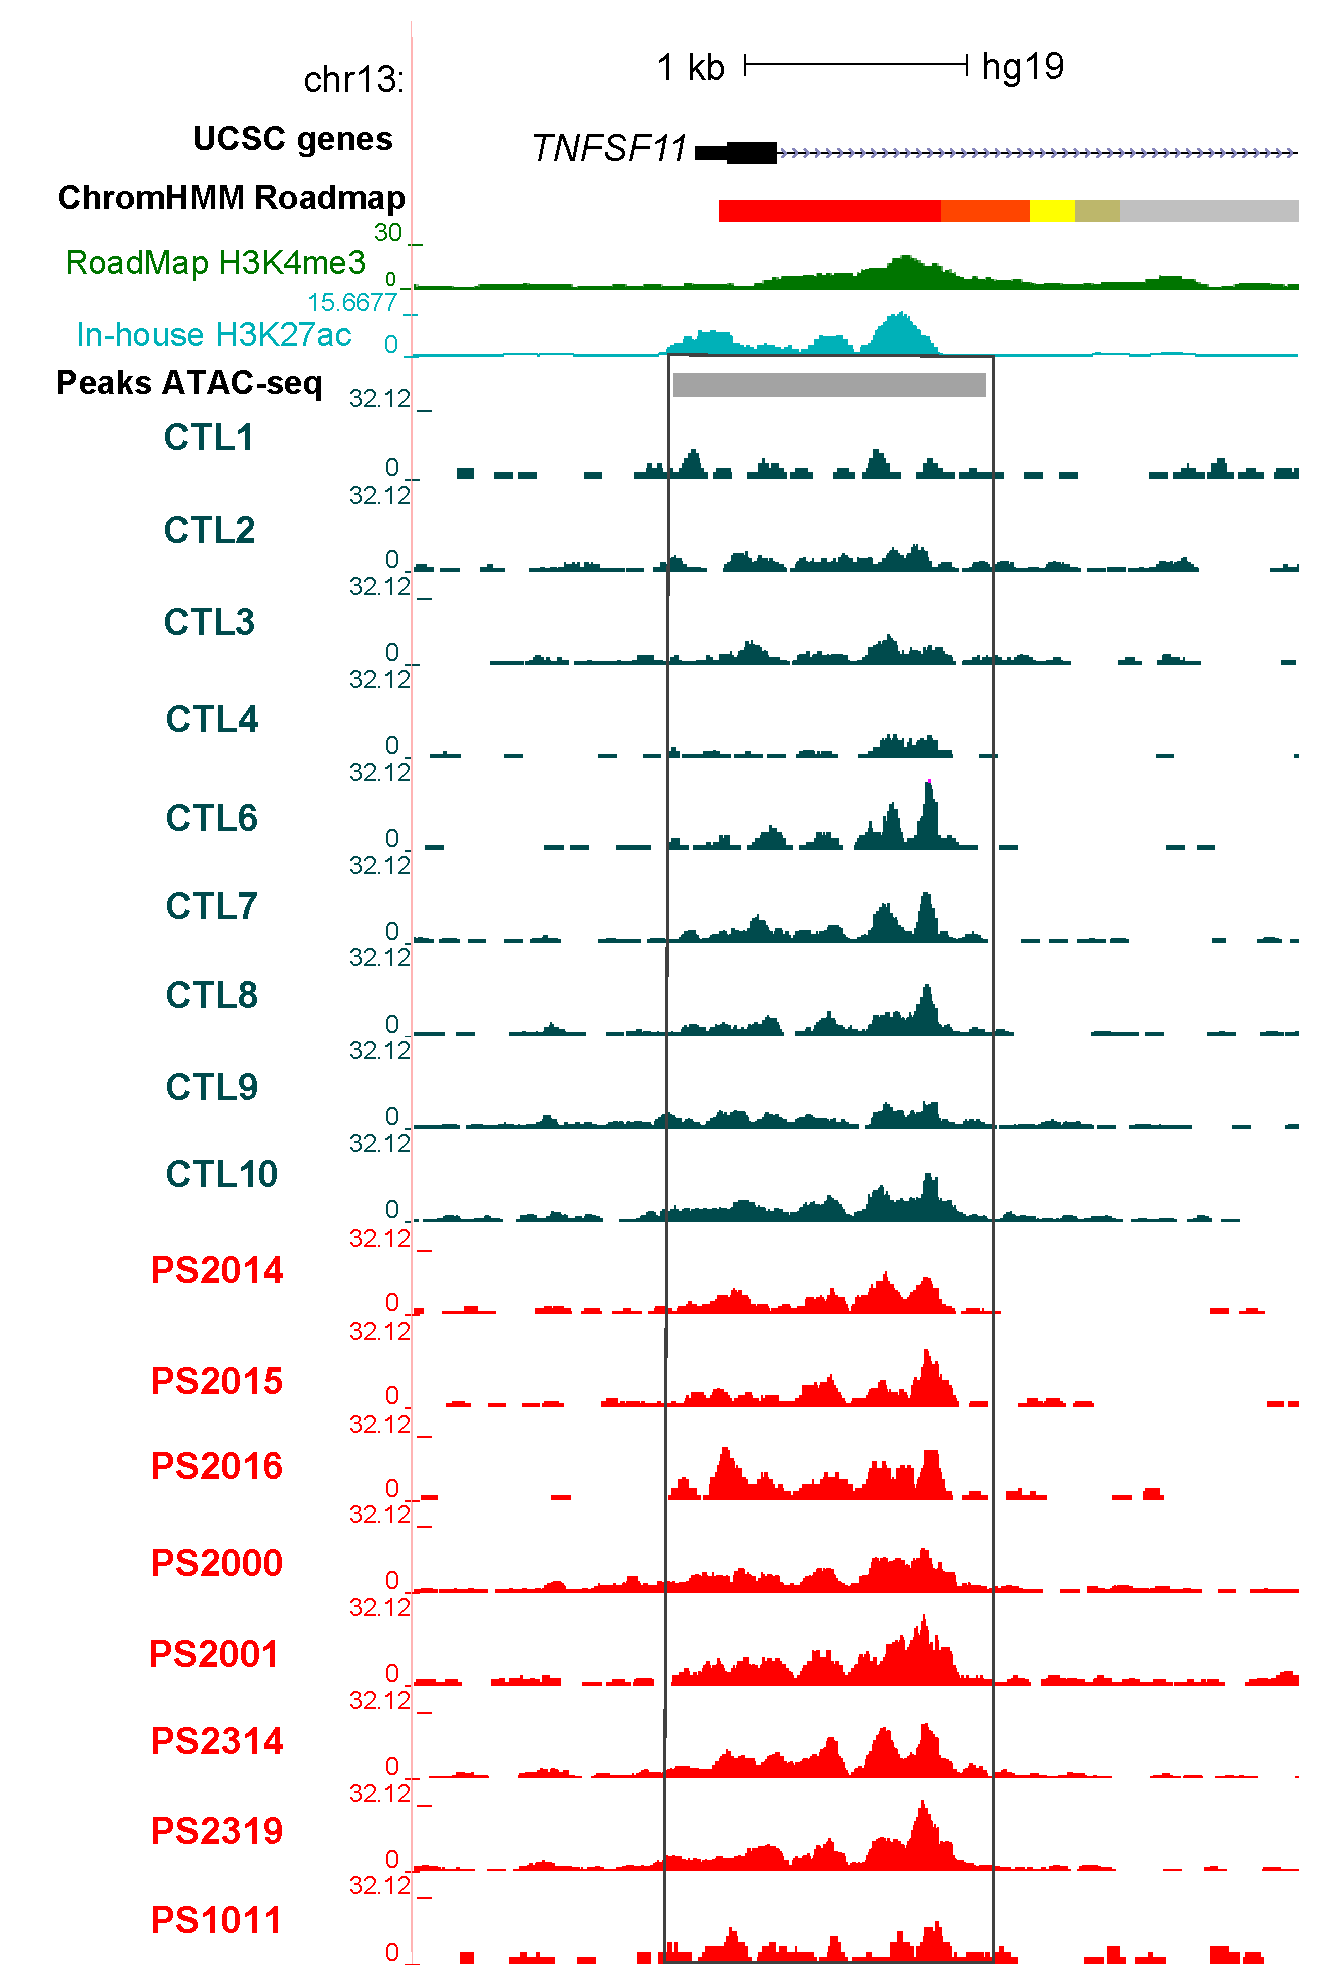
\includegraphics[width=\textwidth]{./Results2/pdfs/UCSC_ATAC_CD8_peak_prom_TNFSF11}
\caption{\textbf{}}
% The percentage sign indicated that the other subfig goes side by side
\end{subfigure}%
\begin{subfigure}{0.45\textwidth}
\centering
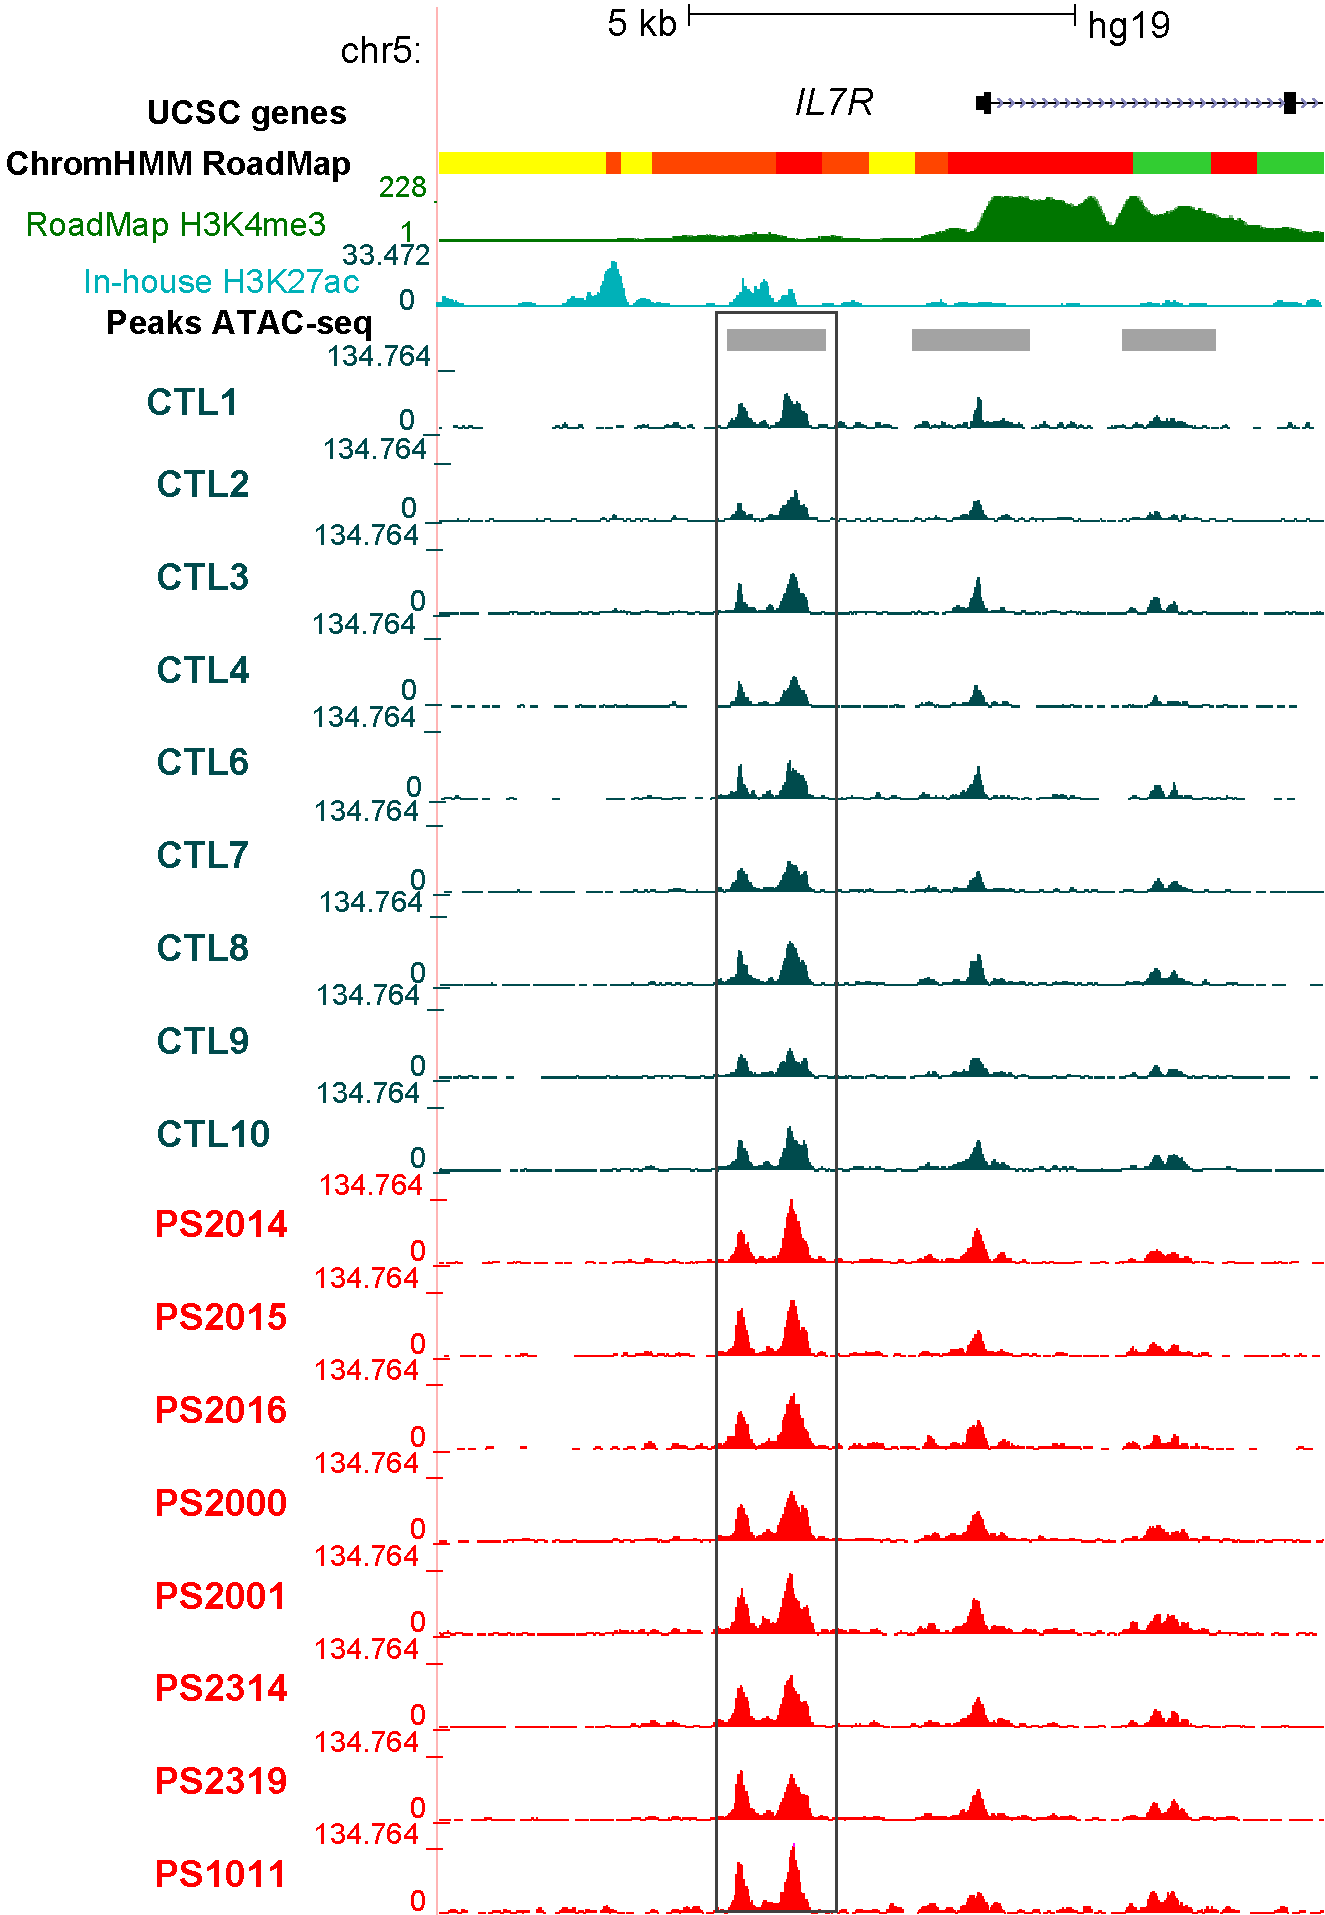
\includegraphics[width=\textwidth]{./Results2/pdfs/UCSC_ATAC_CD8_normalised_peak_enh_IL7R}
\caption{\textbf{}}
\end{subfigure}
\caption[Epigenetic landscape at two ATAC differential accessible regions between patients and controls in CD8$^+$ cells.]{\textbf{Epigenetic landscape at two ATAC differential accessible regions between patients and controls in CD8$^+$ cells.} UCSC Genome Browser view illustrating the normalised ATAC read density (y-axis) in DARs located at (A) the promoter of \textit{TNFSF11} gene and (B) up-stream the \textit{IL7R} gene (x-axis). Both DARs were more open in CD8$^+$ cells from psoriasis compared to controls. Tracks are colour-coded by condition: control (CTL)=dark turquoise and psoriasis (PS)=red. The Roadmap Epigenomics Project chromatin segmentation map and H3K4me3 for CD8$^+$ cells are also shown, together with a representative track from the in-house ChIPm H3K27ac in this cell type. All DARs were significant based on FDR$<$0.05 and no fold change cut-off.}
\label{figure:ATAC_PS_CTL_CD8_TNFSF11_IL7R_tracks}
\end{figure} 



%Both of them are relevant genes in driving and maintaining the inflammatory response. For example, \textit{TNFSF11} is a cytokine from the TNF family involved in the regulation of T cell-dependent immune response and osteoclast differentiation in RA and PsA \parencite{Miranda‐Car\'ús2006,Ritchlin2003}. \textit{TNFSF11} is also downstream the lead SNPs for a CD risk locus \parencite{ImmunoBase}. Interestingly, the \textit{TNFSF11} protein, RANKL was found to be overexpressed in epidermis from psoriasis patients compared to controls and cutaneous lupus erythematosus, highlighting the role of this gene in the pathophysiology of psoriasis \parencite{Toberer2011}. On the other hand \textit{IL7R} is a proximal gene to SLE and MS, amongst others, and the axis IL-7/IL-7R has been found to drive IL7 indepdendent TNF-$\alpha$ inflammation in RA patients presenting iTNF resistence \parencite{van Roon2017}. 
Other interesting CD8$^+$ DARs were found nearby \textit{MAP3K7CL} and \textit{NFKB1} genes, but they did not co-localised with regions annotated as enhancers or transcribed into eRNAs.

%Additionally, none of the CD8$^+$ DARs were found within an LD block (r$^2$$\geq$0.8) of the psoriasis risk GWAS loci.

\subsubsection{Integration of H3K27ac ChIPm and ATAC-seq chromatin accessibility profiles}

%Although a very low number of differentially H3K27ac modified and DARs were found between psoriasis and control samples in the four cell types , commonalities in the disease specific changes were investigated. 
Integration of the observed H3K27ac ChIPm and ATAC differential analysis between patients and controls only showed co-localisation for one region in CD8$^+$ cells. Namely, an intron of the D-tyrosyl-tRNA deacylase 1 (\textit{DTD1}) gene showed lower levels of H3K27ac and chromatin accessibility in psoriasis patients when compared to healthy controls (Figure \ref{figure:ATAC_ChIPm_overlap_DTD1_region_track}). This differential region was annotated as an active enhancer by the Roadmap Epigenomics Project segmentation map and did not interact with the promoter of any gene in CD8$^+$ cells according to Hi-C and promoter Hi-C  data \parencite{Javierre2016}. Interestingly, SNPs within this region are reported to be eQTL for \textit{DTD1} in whole blood (\url{https://gtexportal.org/home/eqtls}). 

%This gene has been described to play a role in the initiation of DNA replication and has been associated with aspirine-intolerance in asthmatics \parencite{Pasaje2011}. However, no studies have yet highlighted a direct link of this gene with the pathophysiology of chronic inflammatory diseases.  

\begin{figure}[htb]
\centering
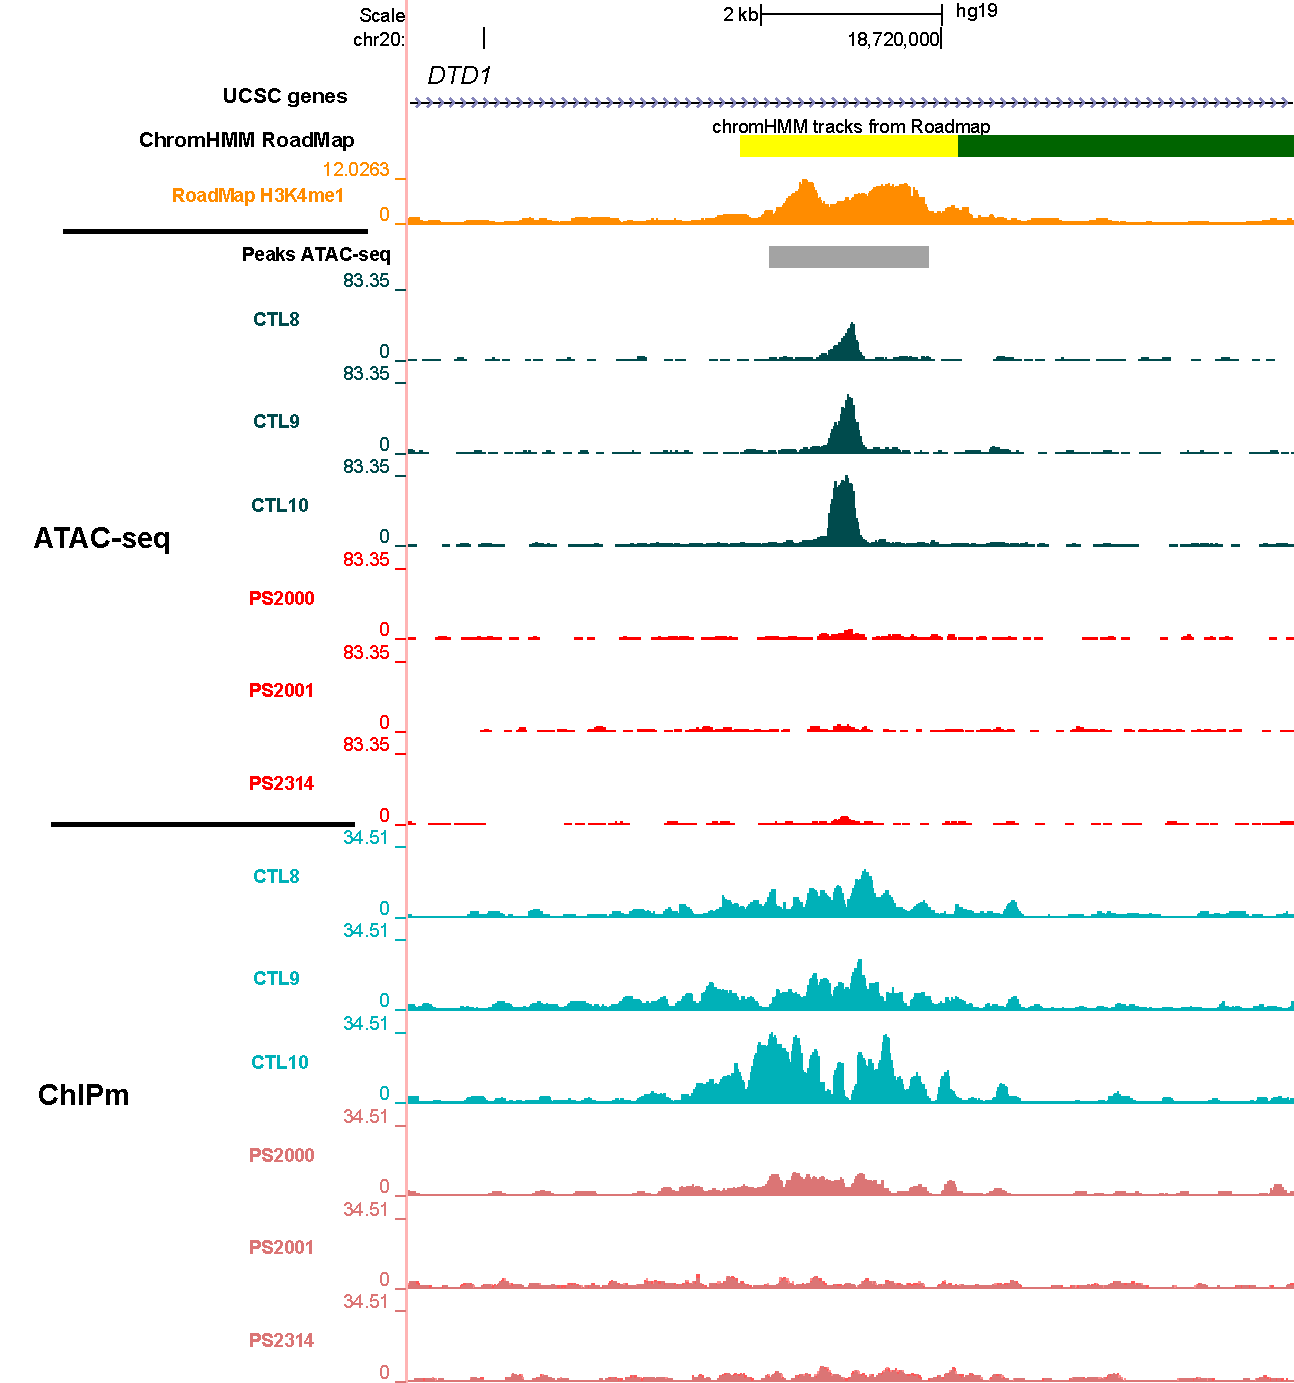
\includegraphics[width=0.6\textwidth]{./Results2/pdfs/ChIPm_H3K27ac_UCSC_CD8_DTD1_track}
\caption[Epigenetic landscape at \textit{DTD1} locus showing differential H3K27ac and chromatin accessibility between psoriasis patients and controls in CD8$^+$ cells.]{\textbf{Epigenetic landscape at \textit{DTD1} locus showing differential H3K27ac and chromatin accessibility between psoriasis patients and controls in CD8$^+$ cells.} UCSC Genome Browser view illustrating the normalised ATAC read density and H3K27ac normalised fold-enrichment (y-axis). Tracks are colour-coded by condition and assay: control (CTL)=dark and light turquoise and psoriasis (PS)=light and dark red, for ATAC and ChIPm respectively. The Roadmap Epigenomics Project chromatin segmentation map and H3K4me1 for CD8$^+$ cells are also shown.}
\label{figure:ATAC_ChIPm_overlap_DTD1_region_track}
\end{figure}




\subsection{Differential gene expression analysis in circulating immune cells in psoriasis}



\subsubsection{Data processing and quality control}

In addition to characterising the chromatin accessibility landscape, gene expression profiles in psoriasis and healthy individuals were analysed  by RNA-seq in the same four primary circulating immune cell types (Table \ref{tab:Psoriasis_cohort_metadata}). All 72 samples showed percentages of RNA-seq reads mapping to a unique location in the genome above the recommended 70-80\% (Figure \ref{figure:RNAseq_mapping_rate_and_reads_in_genes}A). After filtering, all samples had at least 20 million reads (as required by ENCODE standards) mapping to a comprehensive list of Ensembl features, including protein coding genes and lncRNAs (Figure \ref{figure:RNAseq_mapping_rate_and_reads_in_genes}B). %The median total reads mapping to Ensembl features was greater for CD14$^+$ monocytes when compared to the other three cell types. 
In all four cell types, greater mapping rates and total reads mapping to Ensembl features were observed for cohort 1B samples when compared to cohort 1A. These differences were attributed to the library preparation and sequencing of each cohort in two batches.  

PCA using normalised reads showed that most of variability was driven by cell type differences, with three main clusters corresponding to CD14$^+$ monocytes, CD4$^+$ and CD8$^+$ T cells, and CD19$^+$ cells (Figure \ref{figure:RNAseq_PCA_all}). Within each cell type cluster, samples were further grouped by cohort (1A and 1B) but not by condition (psoriasis and control) (Figure \ref{figure:RNAseq_heat_map}). In fact, PC4 (explaining 3\% of the total variance) from the PCA correlated with batch and clearly separated the 72 samples into cohort 1A and 1B (Figure \ref{figure:ATAC_RNAseq_batch_effect}B). 


%\begin{figure}[htbp]
%\centering
%\begin{subfigure}{0.7\textwidth}
%\centering
%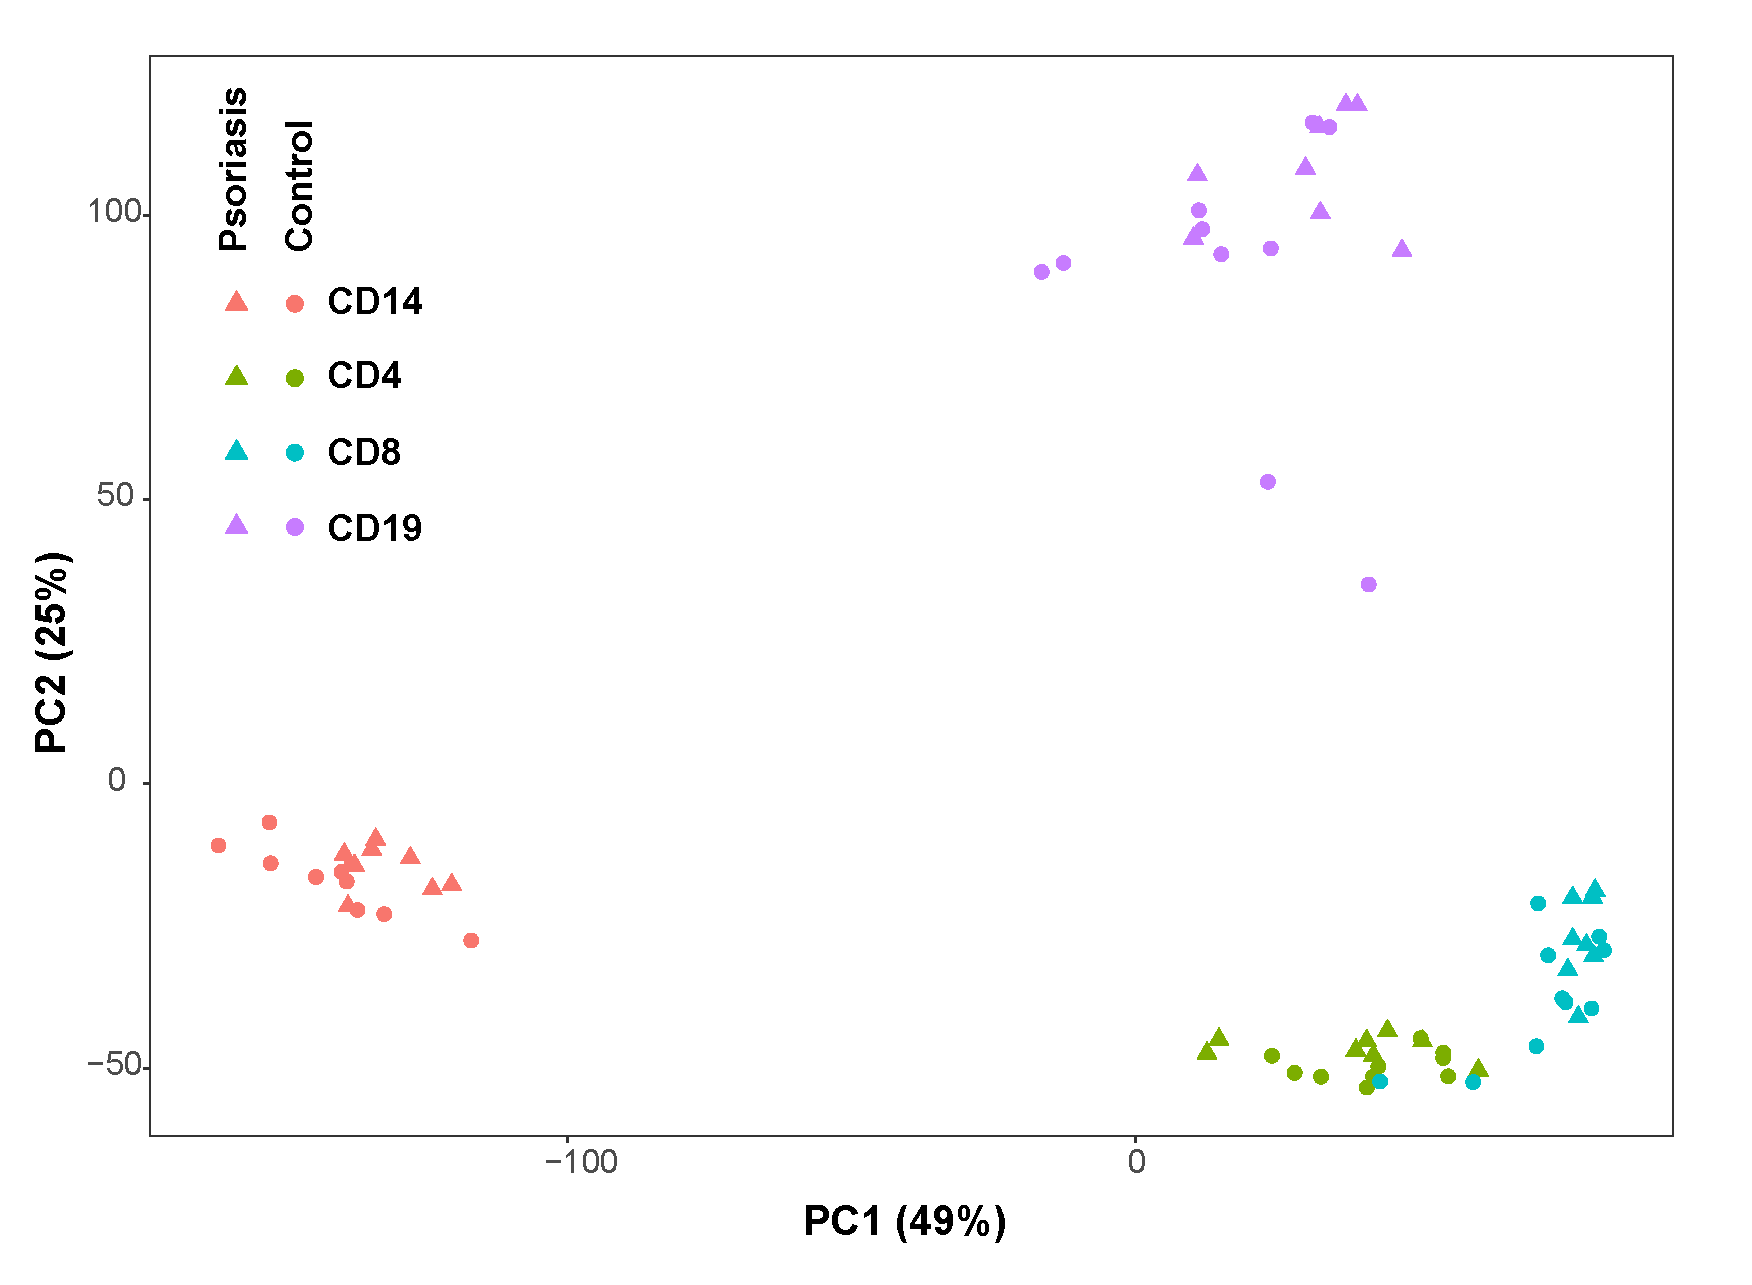
\includegraphics[width=\textwidth]{./Results2/pdfs/PS_CTL_all_samples_varied_PCA1and2_plot}
%\caption{\textbf{}}
%% The percentage sign indicated that the other subfig goes side by side
%\end{subfigure}
%\begin{subfigure}{0.7\textwidth}
%\centering
%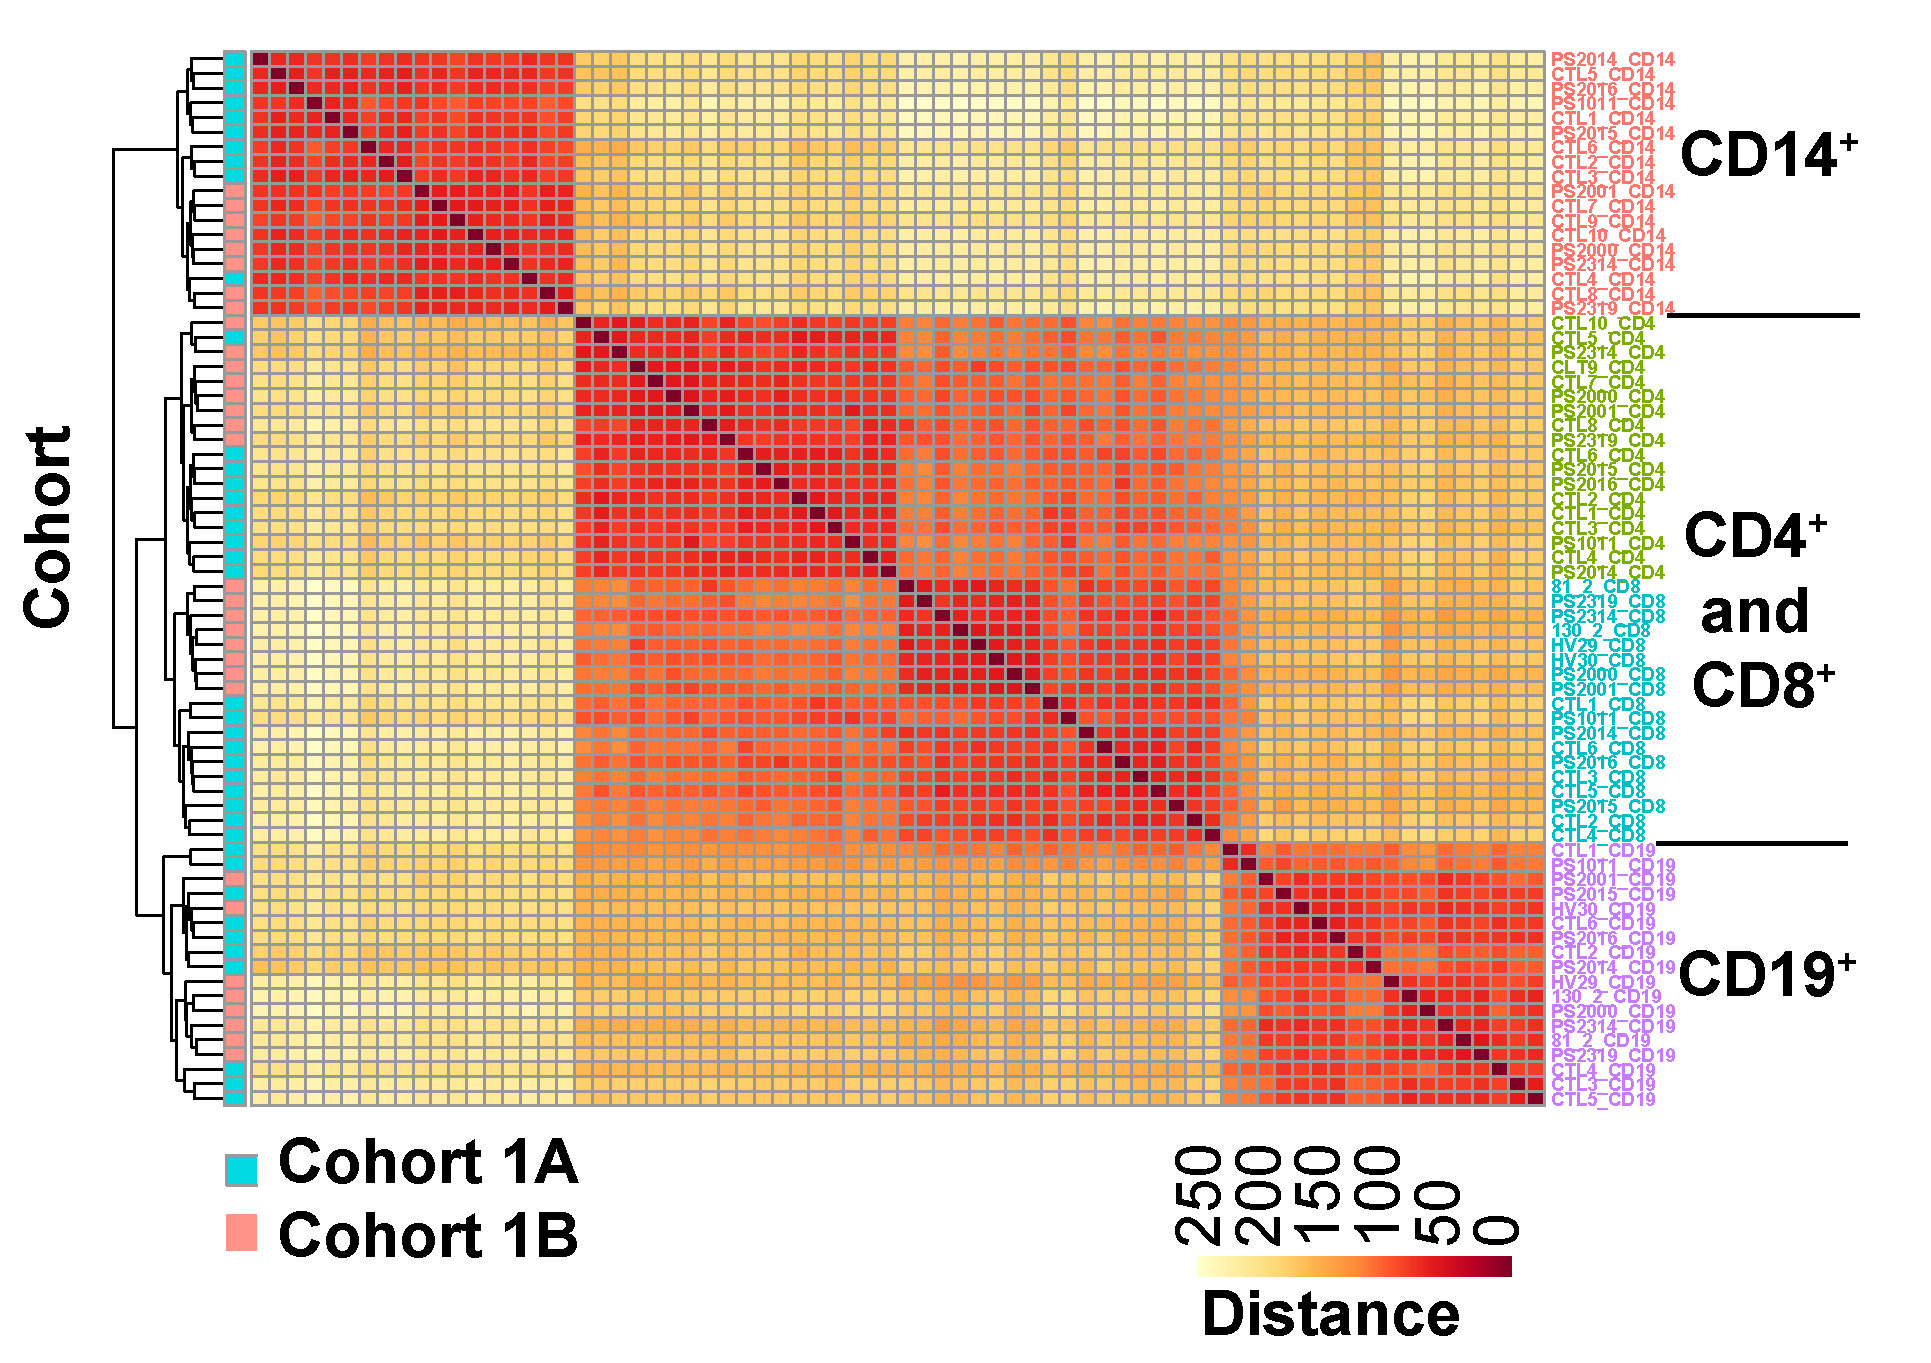
\includegraphics[width=\textwidth]{./Results2/pdfs/PS_CTL_all_samples_heatmap_including_batch}
%\caption{\textbf{}}
%\end{subfigure}
%\caption[PCA and sample distance heatmap with hierarchical clustering illustrating the sample variability based on the gene expression profiles for all 72 samples.]{\textbf{PCA and sample distance heatmap with hierarchical clustering illustrating the sample variability based on the gene expression profiles for all 72 samples.} (A) The first and second PCs (x-axis and y-axis, respectively), where each point represents a sample, colour coding for cell type and the shape for cohort (batch). The proportion of variation explained by each principal component is indicated.(B) Distance matrix built based on normalised read counts mapping to 20,493 Ensembl featured remaining after appropriate filtering followed by hierarchical clustering of the samples. Additional annotation of the clustering based on cohort identity is included on the left hand side.}
%\label{figure:RNAseq_PCA_and_heat_map}
%\end{figure}



\begin{figure}[htbp]
	\centering
	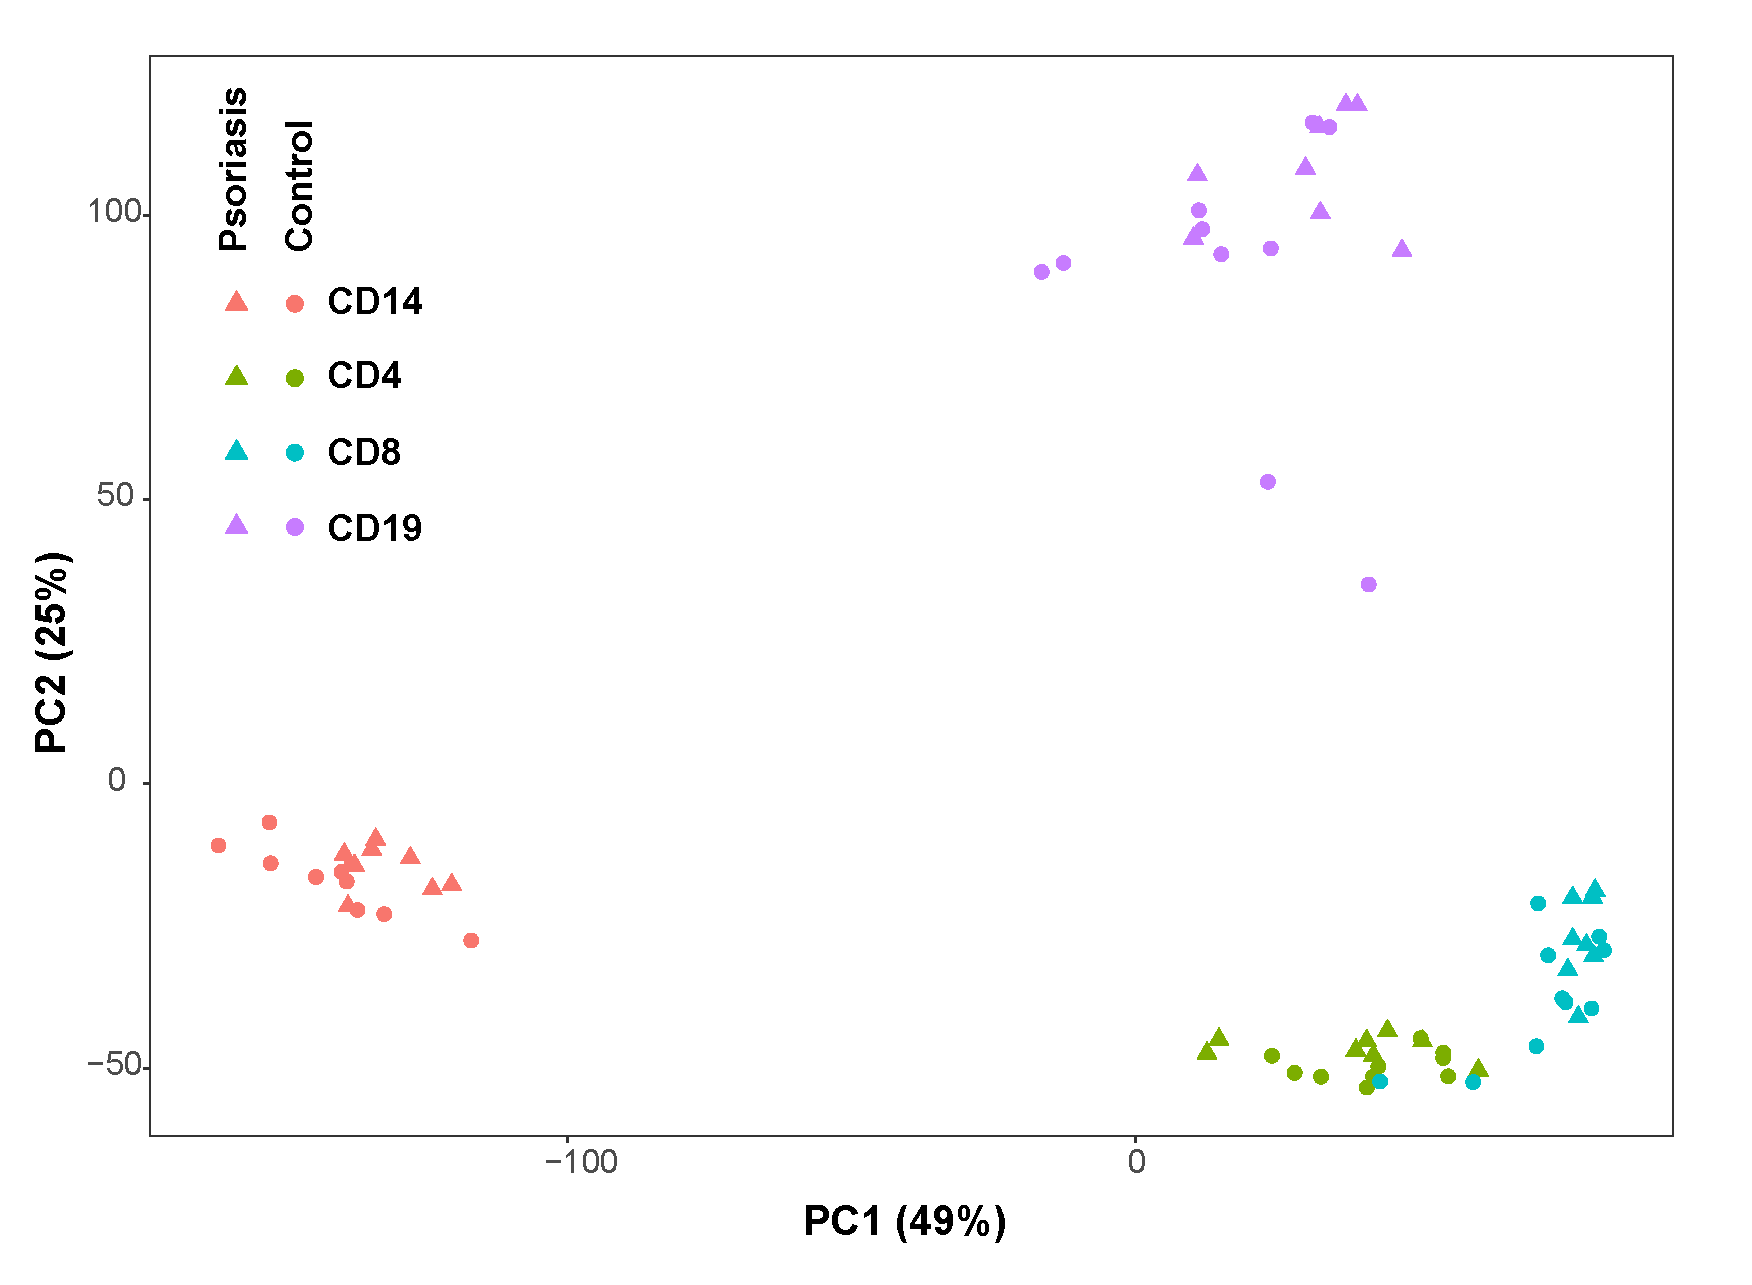
\includegraphics[width=0.6\textwidth]{./Results2/pdfs/PS_CTL_all_samples_varied_PCA1and2_plot}
	\caption[PCA illustrating the sample variability based on the gene expression profiles for all 72 samples.]{\textbf{PCA illustrating the sample variability based on the gene expression profiles for all 72 samples.} The first and second PCs (x-axis and y-axis, respectively), where each point represents a sample, colour coding for cell type and the shape for cohort (batch). The proportion of variation explained by each principal component is indicated.}
	\label{figure:RNAseq_PCA_all}
\end{figure}


\subsubsection{mRNA and lncRNA differential expression analysis}

Differential gene expression analysis between eight psoriasis patients and ten healthy controls was performed using DESeq2 and including cohort identity as a covariate to account for the aforementioned batch effect. For each cell type, differentially expressed mRNAs were identified using two thresholds: FDR $<$0.05 and FDR $<$0.01 (Table \ref{tab:RNAseq_PS_CTL_differential_analysis_results}). CD14$^+$ monocytes and CD8$^+$ T cells showed the largest number of differentially expressed mRNAs between psoriasis patients and controls with the highest magnitude of fold change (Figure \ref{figure:RNAseq_PS_CTL_volcano_plots}). %The more dysregulated gene expression response between patients and controls found in circulating psoriasis CD8$^+$ when compared to the CD4$^+$ may suggest the same hypothesis as in skin, where CD8$^+$ are considered the main effector cells undergoing activation upon the inflammatory stimuli \parencite(Nickoloff1999). Interestingly, CD19$^+$ presented a greater number of differentially expressed mRNAs than CD4$^+$. %regardless of their not yet having been implicated in disease (confirm).

CD14$^+$ monocytes and CD4$^+$ T cells presented similar numbers of genes up-regulated and down-regulated in psoriasis patients when compared to the healthy controls. In contrast, for CD8$^+$ and CD19$^+$ cells a larger number of modulated genes were down-regulated in patients compared to controls. In CD14$^+$ monocytes, the most significant up-regulated genes (fold change$>$1.5) included \textit{SDC2}, \textit{CD83} and \textit{MIR22G} (Figure \ref{figure:RNAseq_PS_CTL_volcano_plots}A). In CD8$^+$, \textit{SOCS3} and \textit{CXCR4}  were amongst the top differentially expressed genes with fold change$>$1.5 (Figure \ref{figure:RNAseq_PS_CTL_volcano_plots}C), whereas  in CD4$^+$ cells, the G protein-coupled receptor \textit{GPR18} showed the most significant down-regulation with a fold change=1.4.  Overall, the dysregulation of gene expression in psoriasis patients compared to controls in all four analysed cell types demonstrated to be moderate. 

\begin{table}[htbp]
%\setlength{\tabcolsep}{20pt} only to stretch the columns if you want
%\renewcommand{\arraystretch}{1.5}
\centering
\begin{tabular}{@{} c c c c c}
\toprule
\textbf{Cell type}   & \textbf{mRNA}            & \textbf{lncRNA}           & \textbf{Up-regulated}        & \textbf{Down-regulated}\\
                     & \textbf{FDR$<$0.05/0.01} & \textbf{FDR$<$0.05/0.01}  & \textbf{FDR$<$0.05/0.01}    & \textbf{FDR$<$0.05/0.01}\\
	
										
\midrule
\midrule
CD14$^+$             & 671/229                  & 28/8                    & 331/112                       &368/125\\               
CD4$^+$              & 108/40                   & 12/4                    & 56/20                         &64/24 \\
CD8$^+$              & 651/175                  & 31/5                    & 269/67                        &418/113 \\
CD19$^+$             & 167/71                   & 6/2                     & 29/13                         &144/60\\
\bottomrule 
\end{tabular}
\medskip %gap
\caption[Summary results from the differential gene expression analysis between psoriasis patients and healthy controls in CD14$^+$ monocytes, CD4$^+$, CD8$^+$ and CD19$^+$ cells.]{\textbf{Summary results from the differential gene expression analysis between psoriasis patients and healthy controls in CD14$^+$ monocytes, CD4$^+$, CD8$^+$ and CD19$^+$ cells.} The number of statistically differentially expressed mRNAs and lncRNAs are listed for two FDR threshold (FDR$<$0.05 and FDR$<$0.01). No threshold for the fold change was applied in this analysis. For each of the FDR threholds the number of up- and down- regulated genes is included.}
\label{tab:RNAseq_PS_CTL_differential_analysis_results}
\end{table}
\bigskip %bigger spac


None of the genes coding for well-known psoriasis drug targets, such as TNF-$\alpha$, IL-17 and IL-6, were up-regulated in any of the four cells types in psoriasis patients compared to healthy controls. CD8$^+$ showed the largest number of significant DEGs (FDR$<$0.05) overlapping putative psoriasis GWAS genes from the NHGRI-EBI catalog (\url{https://www.ebi.ac.uk/gwas}) (Table \ref{tab:RNAseq_PS_CTL_GWAS_overlap}, 7 hits), followed by CD14$^+$ monocytes and CD4$^+$ cells (3 hits each). Some of the GWAS genes were found to be differentially expressed in more than one cell type, including \textit{NFKBIA}, \textit{TNFAIP3}, \textit{B3GNT2} and \textit{NFKBIZ} (Table \ref{tab:RNAseq_PS_CTL_GWAS_overlap}). Enrichment of psoriasis GWAS genes amongst the DEGs in patients compared to controls was statistically significant only for CD4$^+$ and CD8$^+$ T cells (Fisher exact test, p-values 2.6x10$^{-3}$ and 9.36x10$^{-4}$, respectively).

\begin{figure}[htbp]
\centering
\begin{subfigure}{0.5\textwidth}
\centering
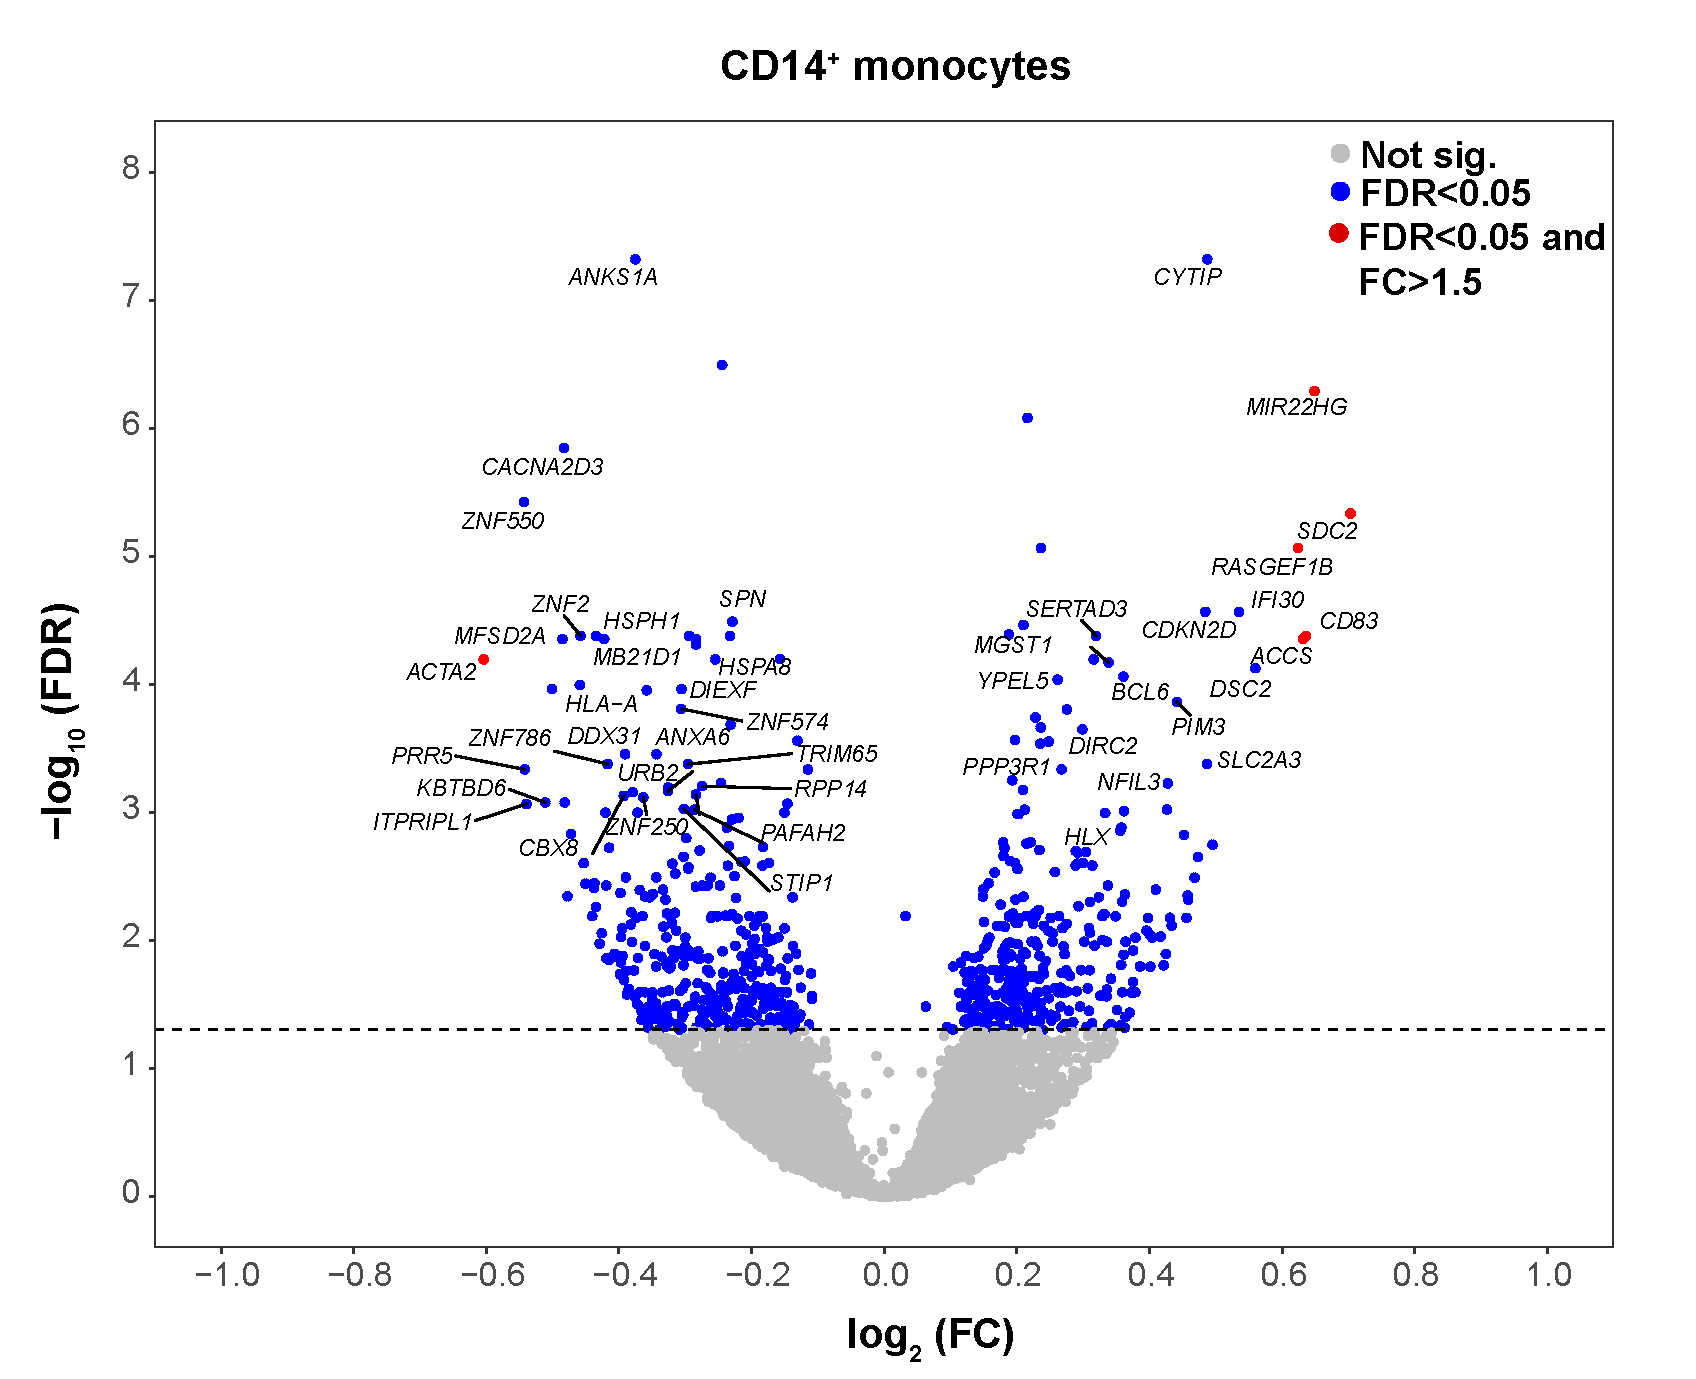
\includegraphics[width=\textwidth]{./Results2/pdfs/RNA_PS_CTL_CD14_volcano_plot}
\caption{\textbf{}}
% The percentage sign indicated that the other subfig goes side by side
\end{subfigure}%
\begin{subfigure}{0.5\textwidth}
\centering
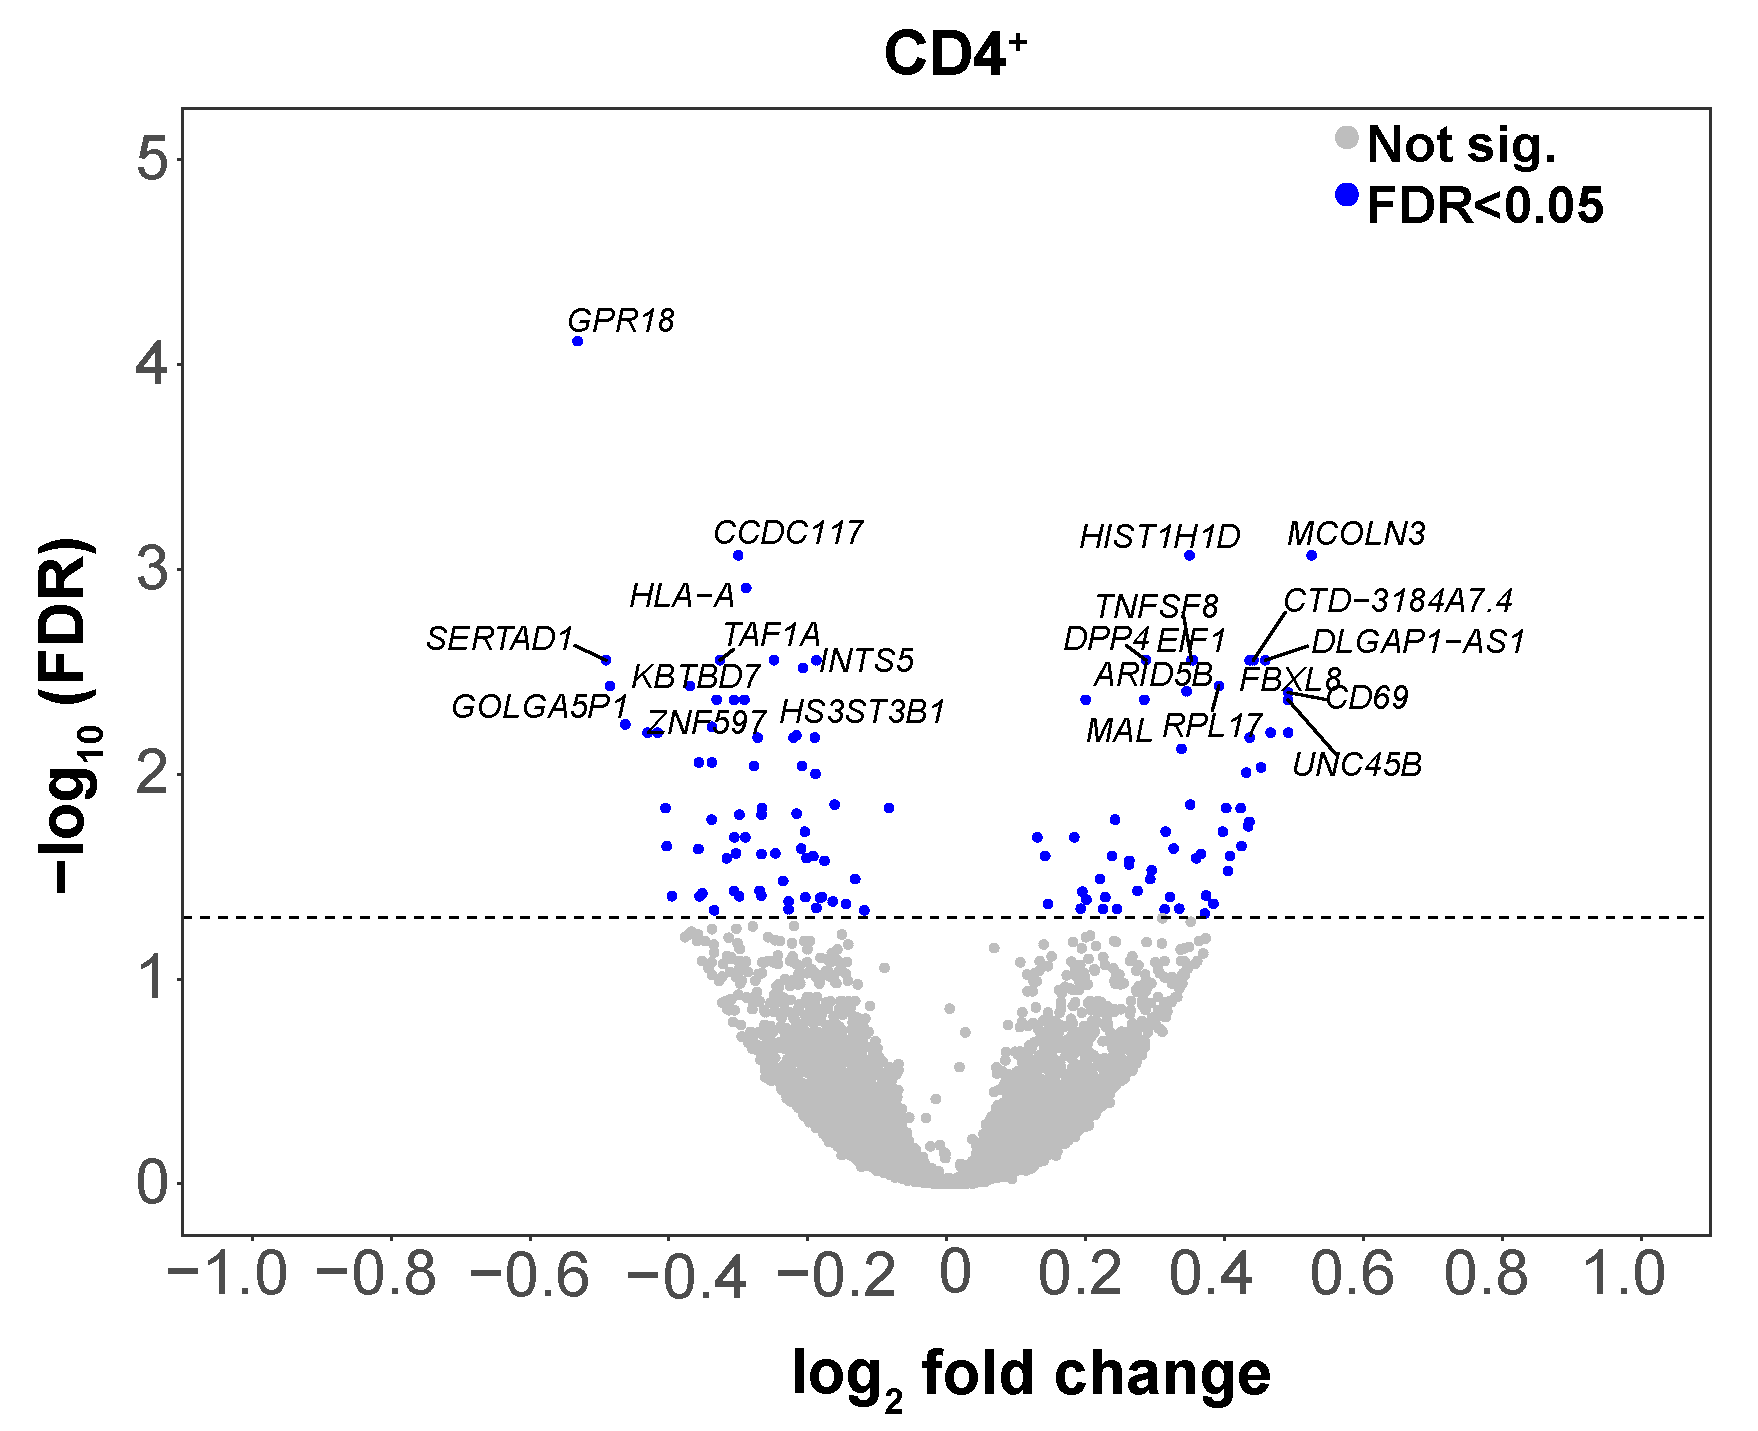
\includegraphics[width=\textwidth]{./Results2/pdfs/RNA_PS_CTL_CD4_volcano_plot}
\caption{\textbf{}}
\end{subfigure}
\begin{subfigure}{0.5\textwidth}
\centering
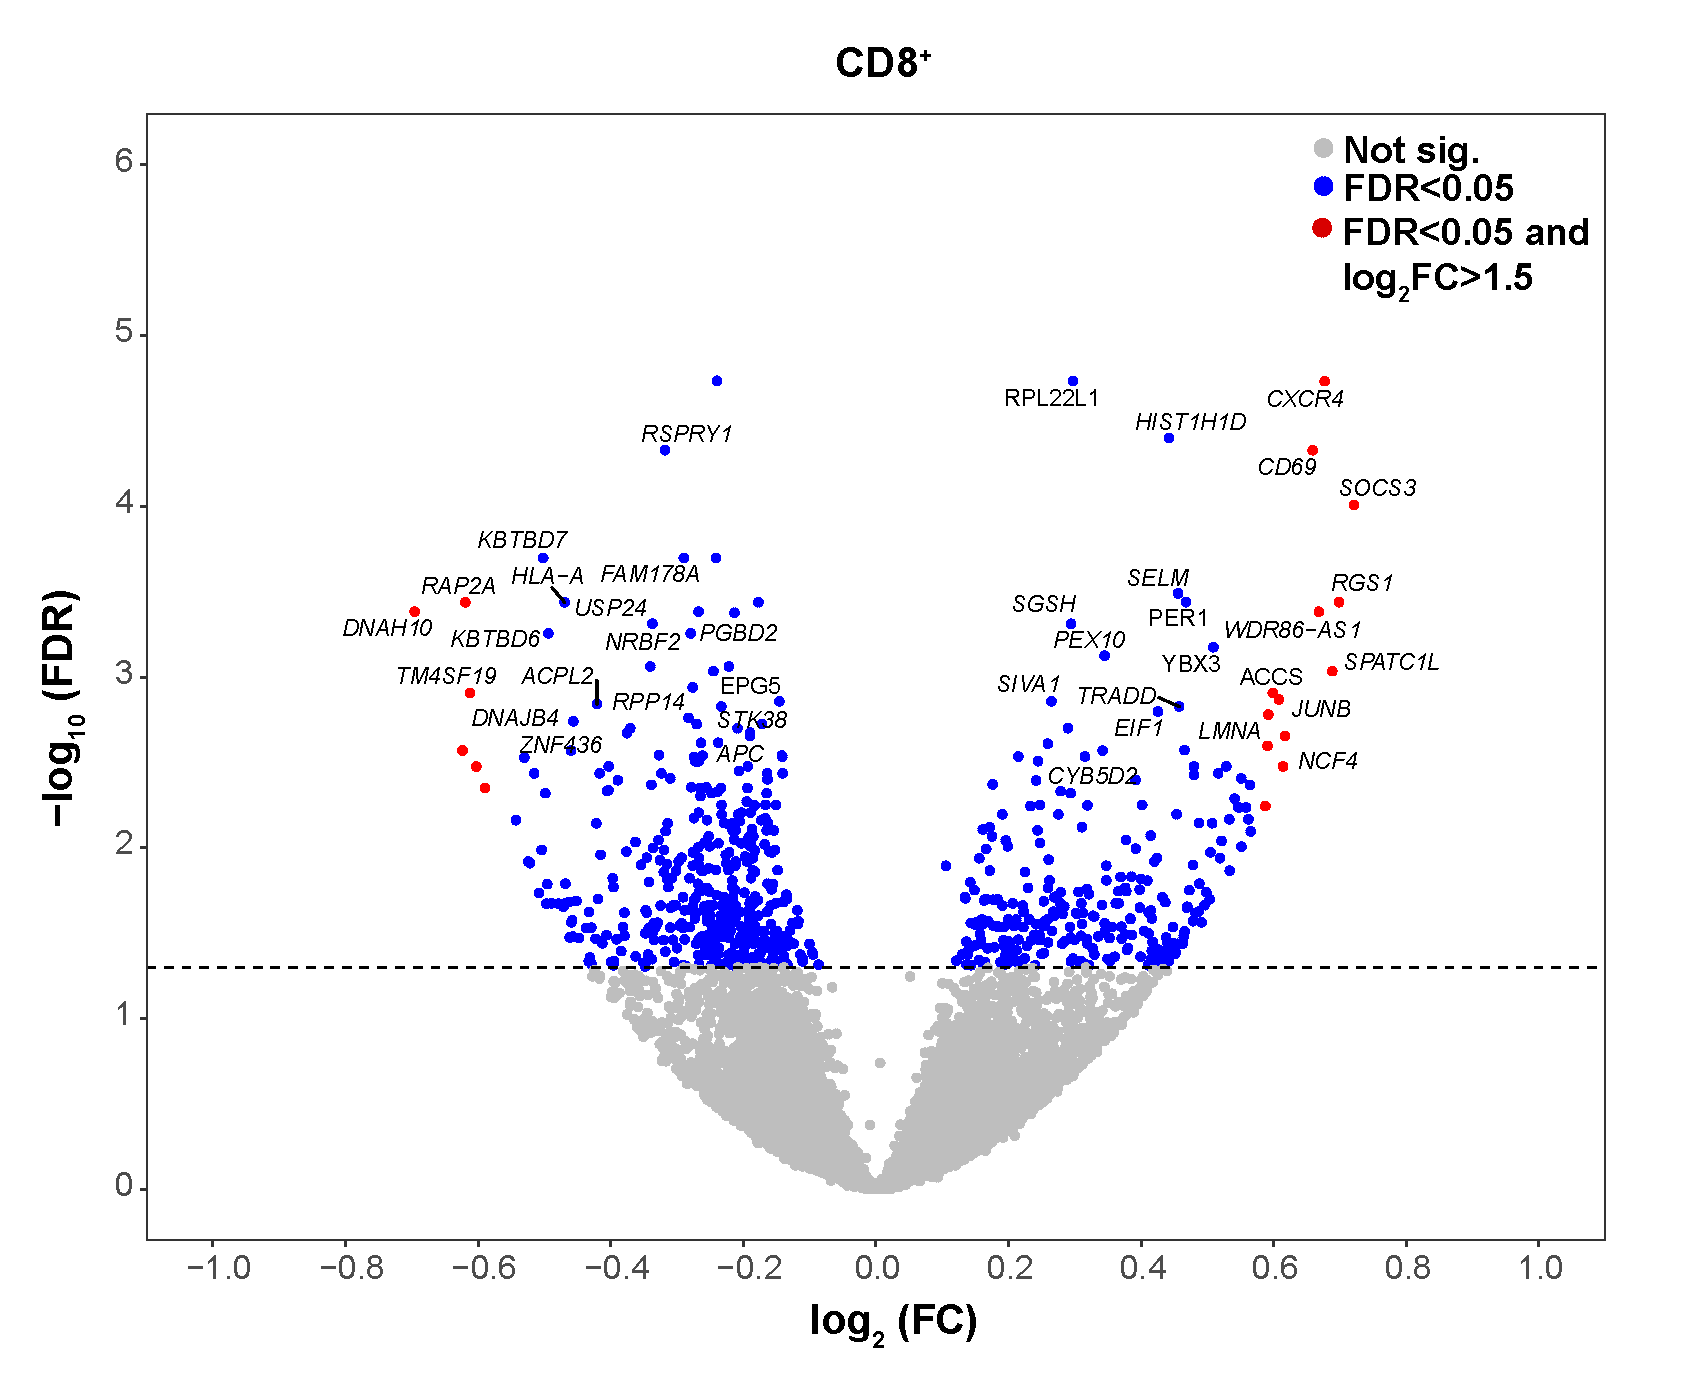
\includegraphics[width=\textwidth]{./Results2/pdfs/RNA_PS_CTL_CD8_volcano_plot}
\caption{\textbf{}}
% The percentage sign indicated that the other subfig goes side by side
\end{subfigure}%
\begin{subfigure}{0.5\textwidth}
\centering
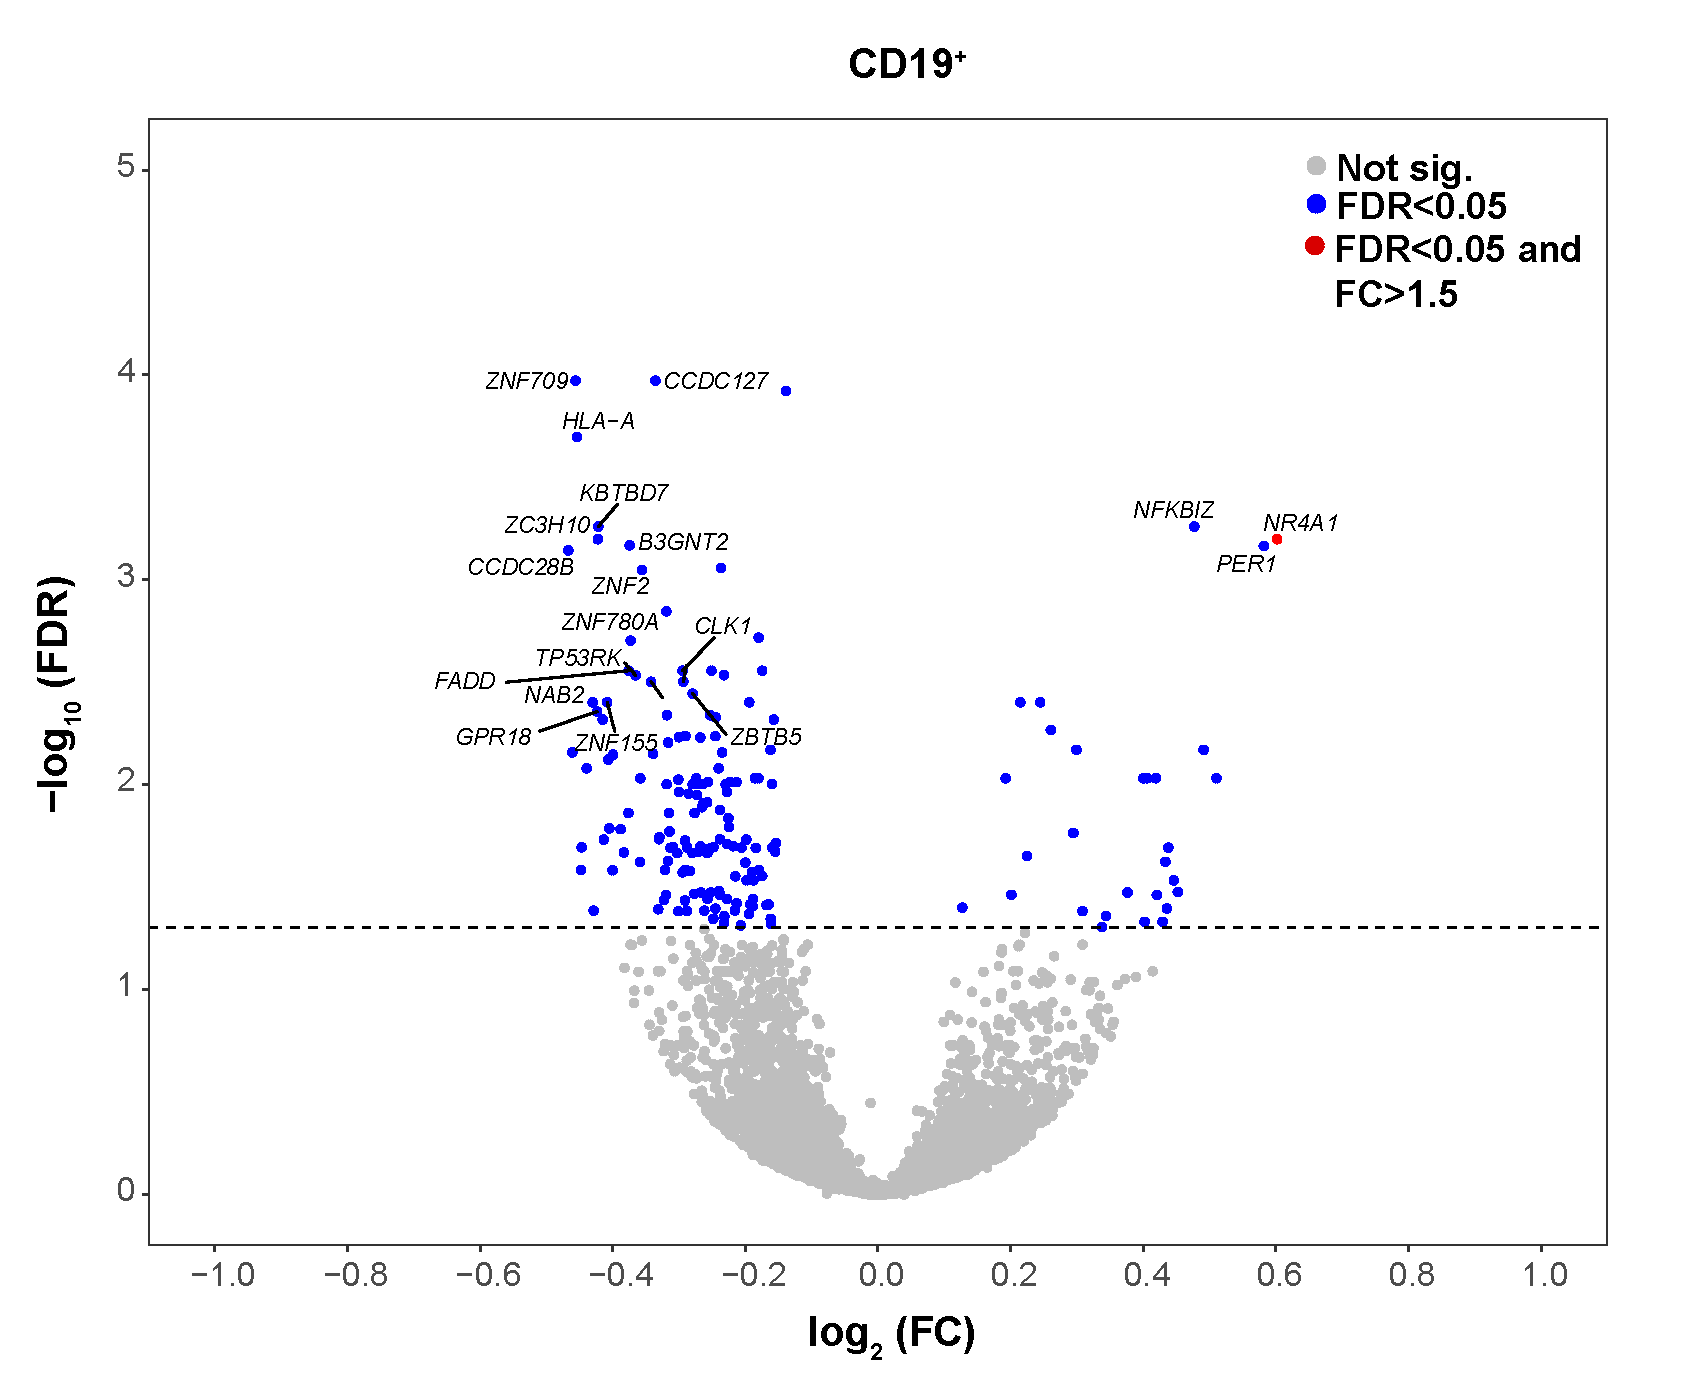
\includegraphics[width=\textwidth]{./Results2/pdfs/RNA_PS_CTL_CD19_volcano_plot}
\caption{\textbf{}}
\end{subfigure}
\caption[Magnitude and significance of gene expression changes between psoriasis patients and healthy controls in four immune cell types.]{\textbf{Magnitude and significance of gene expression changes between psoriasis patients and healthy controls in four immune cell types.} Volcano plots illustrating the differential gene expression analysis results for (A) CD14$^+$ monocytes, (B) CD4$^+$, (C) CD8$^+$ and (D) CD19$^+$ cells. The log$_2$fold change represents change in expression for each gene in the psoriasis group relative to the healthy controls. Significant DEGs (FDR$<$0.05) in blue for fold change$<$1.5 and red for fold change $>$1.5. The volcano plots include mRNAs and lncRNAs species.}
\label{figure:RNAseq_PS_CTL_volcano_plots}
\end{figure} 


%Some of the DEGs across the four cell types overlapped DEGs from the two most comprehensive studies comparing expression of PBMCs isolated from psoriasis patients and healthy controls \parencite{Lee2009,Coda2012}. The greatest overlap (7 genes) was found between the DEGs in CD14$^+$ monocytes and those identified by Coda \textit{et al.}, 2012. However, 5 out of 7 presented opposite directionality. One of those genes dysregulated in the same direction was ubiquitin conjugating enzyme E2 D1 (\textit{UBE2D1}), which mediates, for example, ubiquitination of the TNF receptor-associated factor 6 (TRAF6) protein \parencite{Gru2008}. The greatest overlap with the Lee and colleagues DEGs was found for CD8$^+$ cells (3 genes) in the same direction. Similarly, only one overlap (\textit{NAMPT}) was found with the psoriasis DEGs in a study comparing PBMC transcriptional profiles of three inflammatory diseases (IBD, RA and psoriasis)\parencite{Mesko2010}. The nicotinamide phosphoribosyltransferase\textit{NAMPT}, involved in metabolism and stress response, was up-regulated in our CD14$^+$ monocytes as well as in PBMCs from the three phenotypes studied by Mesko and colleagues, suggesting its role as a marker of inflammation rather than marker for psoriasis.
%For example, CDC like kinase 1 (\textit{CLK1}) involved in protein splicing was downregulated in this CD8$^+$ data set and in the Lee PBMCs in patients when compared to controls and its deficiency has been shown to lead to neuro-inflammation in mice \parencite{Gu2017}. Similarly, only one overlap was found with the psoriasis DEGs in a study comparing PBMC transcriptional profiles of three inflammatory diseases (IBD, RA and psoriasis)\parencite{Mesko2010}. This was for the nicotinamide pPhosphoribosyltransferase (\textit{NAMPT}) gene involved in metabolism and stress response, which was up-regulated in our CD14$^+$ monocytes as well as in PBMCs from psoriasis, IBD and RA patients, suggesting its role as a marker of inflammation rather than marker for psoriasis.




\begin{table}[h]
%\setlength{\tabcolsep}{20pt} only to stretch the columns if you want
\renewcommand{\arraystretch}{0.8}
\centering
\begin{tabular}{@{} c c c c}
\toprule
\textbf{Cell type}   & \textbf{Number of GWAS}   & \textbf{Up-regulated}   & \textbf{Down-regulated}  \\
										 & \textbf{overlaps}         & \textbf{genes}          &\textbf{genes} \\
\midrule
\midrule
CD14$^+$             & 3  & \textit{NFKBIA}                                   & \textit{IL23A}, \textit{FASLG}\\ 
                     &    &                                                   &                                \\                  
CD4$^+$              & 3  & \textit{TNFAIP3}, \textit{NFKBIZ}                 & \textit{FASLG} \\
                     &    &                                                   &                                \\  
CD8$^+$              & 7  & \textit{TNFAIP3}, \textit{NFKBIA}, \textit{ETS1}, & \textit{B3GNT2}, \textit{FASLG} \\ 
                     &    & \textit{SOCS1},\textit{NFKBIZ}                    &  \\ 
										 &    &                                                   &                                \\  
CD19$^+$             & 2  & \textit{NFKBIZ}                                   & \textit{B3GNT2}\\
\bottomrule 
\end{tabular}
\medskip %gap
\caption[Overlap between putative psoriasis GWAS genes and the reported significantly DEGs in CD14$^+$ monocytes, CD4$^+$, CD8$^+$ and CD19$^+$ cells.]{\textbf{Overlap between putative psoriasis GWAS genes and the reported significantly DEGs in CD14$^+$ monocytes, CD4$^+$, CD8$^+$ and CD19$^+$ cells.} DEGs list based on FDR$<$0.05.}
\label{tab:RNAseq_PS_CTL_GWAS_overlap}
\end{table}
\bigskip %bigger spac


\subsubsection{The role of lncRNAs in psoriasis circulating immune cells}

DEGs between psoriasis patients and controls also included lncRNAs in all four cell types. CD8$^+$ and CD14$^+$ monocytes showed the largest number of dysregulated lncRNAs between psoriasis patients and controls (Table \ref{tab:RNAseq_PS_CTL_differential_analysis_results}). 
%In contrast, CD19$^+$ was the cell type showing the lowest number of lncRNAs differentially expressed. 
%The differentially expressed lncRNAs in this study were overlapped with the 259 lncRNAs identified as dysregulated in PBMCs when comparing PsA patients versus healthy controls by Dolcino \textit{et al.}, 2018 (Table \ref{tab:RNAseq_PS_CTL_lncRNAs_annotation}). The largest overlap was found in CD14$^+$ monocytes, where four of the differentially expressed lncRNAs were also reported by Dolcino and colleagues. However, \textit{HOTAIRM1} and \textit{ILF3-AS1} were up-regulated in psoriasis CD14$^+$ monocytes when compared to controls but appeared down-regulated in PsA PBMCs. 

%
%\begin{table}[htbp]
%%\setlength{\tabcolsep}{20pt} only to stretch the columns if you want
%%\renewcommand{\arraystretch}{1.5}
%\centering
%\begin{tabular}{@{} c c c}
%\toprule
%\textbf{Cell type}   & \textbf{LncRNAs with}             &\textbf{LncRNAs overlapping}  \\
                     %& \textbf{functional interactions}  &\textbf{Dolcino \textit{et al.},2018}   \\
%\midrule
%\midrule
%CD14$^+$             & 24  & 4 (\textit{HOTAIRM1}$^{\ast}$, \textit{ILF3-AS1}$^{\ast}$, \\
                     %&     & \textit{MMP24-AS1}, \textit{RP11-325F22.2})\\                 
%CD4$^+$             & 12  & 1 (\textit{MMP24-AS1}) \\
%CD8$^+$             & 21  & 1(\textit{CTB-25B13.12})\\
%CD19$^+$             & 5   & 0\\
%\bottomrule 
%\end{tabular}
%\medskip %gap
%\caption[Functional interactions and overlap with another study for the differentially expressed lncRNAs in each cell type.]{\textbf{Functional interactions and overlap with another study for the differentially expressed lncRNAs in each cell type.}For each cell type the number of differentially expressed lncRNAs (FDR$<$0.05) for which a functional interaction has been experimentally validated based on NPInter database is shown. NPInter documents functional interactions between noncoding RNAs (except tRNAs and rRNAs) and biomolecules (proteins, RNAs and DNAs) which have published experimental validation. This table also records the number of differentially expressed lncRNAs overlapping with the Dolcino \textit{et al.}, 2018 study, where PBMCs from PsA patients and healthy controls are contrasted.($^{\ast}$) indicates dysregulation in the opposite direction between this data and Dolcino \textit{et al.}.}
%\label{tab:RNAseq_PS_CTL_lncRNAs_annotation}
%\end{table}
%\bigskip %bigger spac

The majority of differentially expressed lncRNAs (FDR$<$0.05) had an experimentally validated functional interacting partner based on the database NPInter (Table \ref{tab:RNAseq_PS_CTL_lncRNAs_annotation}), which retrieves published functional interactions between non-coding RNAs and biomolecules (proteins, RNAs and DNAs) \parencite{Hao2016}. Some of these lncRNAs were previously found to be differentially expressed in PBMCs when comparing PsA patients vs healthy controls in a study conducted by Dolcino and colleagues \parencite{Dolcino2018} (Table \ref{tab:RNAseq_PS_CTL_lncRNAs_annotation}). Examples of cell type-specific differentially expressed lncRNAs between psoriasis patients and healthy controls included \textit{DYNLL1-AS1} (or \textit{NAV}), \textit{HOTAIRM1} and \textit{NEAT1} in CD14$^+$ monocytes, \textit{DLGAP1-AS1} in CD4$^+$, \textit{UBXN8} and \textit{MIR146A} in CD8$^+$ and \textit{LINC00324} in CD19$^+$. Only \textit{RP11-218M22.1} was dysregulated between psoriasis and healthy controls in all four cell types. 

Cell-type specific dysregulated lncRNAs included down-regulation of \textit{DYNLL1-AS1} (fold change=0.78) in CD14$^+$ monocytes from psoriasis patients. \textit{DYNLL1-AS1} has been shown to affect histone modifications of critical IFN-stimulated genes (ISGs), including \textit{IFITM3} and \textit{MxA}, leading to their transcriptional down-regulation \parencite{Ouyang2014}. Despite down-regulation of \textit{DYNLL1-AS1}, up-regulation of \textit{IFITM3} and \textit{MxA} was not observed in psoriasis CD14$^+$ monocytes in this data. Conversely, \textit{HOTAIRM1} up-regulation (fold change=1.23) in CD14$^+$ monocytes from psoriasis patients (Figure \ref{figure:RNAseq_PS_CTL_CD14_expression_HOTAIRM_UPF1}A) was accompained by down-regulation of its NPInter experimentally validated target \textit{UPF1} (fold change=0.87), a gene coding for a RNA helicase and ATPase protein \parencite{Hao2016} (Figure \ref{figure:RNAseq_PS_CTL_CD14_expression_HOTAIRM_UPF1}B). Lastly, \textit{NEAT1} expression was up-regulated (fold change=1.27) in psoriasis patients compared to controls in CD14$^+$ monocytes and has also been reported to be up-regulated in SLE CD14$^+$ monocytes when compared to healthy individuals \parencite{Zhang2016}.

%The negative regulator of antiviral response \textit{DYNLL1-AS1} (or \textit{NAV}), which has been shown to affect the histone modifications of some critical IFN-stimulated genes (ISGs), such as \textit{IFITM3} and \textit{MxA} leading to down-regulation of their expression \parencite{Ouyang2014}. In this data, \textit{DYNLL1-AS1} was down-regulated indicating lack of one of the negative regulators of the IFN response, notwithstanding the reverse  IFN-$\gamma$ signature observed in the pathway enrichment analysis. Another interesting dysregulated lncRNA in CD14$^+$ monocytes was the HOXA transcript antisense RNA myeloid-specific 1\textit{HOTAIRM1}. In a study using PsA PBMCs \textit{HOTAIRM1} was found to be down-regulated and connected to the expression of the RNA helicase and ATPase \textit{UPF1} \parencite{Dolcino2018}. \textit{UPF1} is involved in nonsense-mediated decay and in partnership with the monocyte chemotactic protein-1-induced protein-1 (\textit{MCPIP1}) gene drives degradation of inflammation-related mRNAs to ensure maintenance of homeostasis \parencite{Mino2015}. In this present study, \textit{HOTAIRM1} appeared to be up-regulated in the CD14$+$ monocytes from psoriasis patients (Figure \ref{figure:RNAseq_PS_CTL_CD14_expression_HOTAIRM_UPF1} (A) and this was consistent with significant down-regulation of \textit{UPF1} in the same cell type (Figure \ref{figure:RNAseq_PS_CTL_CD14_expression_HOTAIRM_UPF1} b), suggesting impairment of this homeostatic mechanisms in the psoriasis patients. The last relevant lncRNA differentially expressed in monocytes was \textit{NEAT1}, which was up-regulated in the patients  compared to the controls. \textit{NEAT1} has been reported to also be up-regulated in SLE CD14$^+$ monocytes and knocking it down has revealed impairment of the TLR-4 signalling and down-regulation of inflammatory genes including IL-6 and CXCL10 \parencite{Zhang2016}.


 \begin{figure}[htbp]
\centering
\begin{subfigure}{0.45\textwidth}
\centering
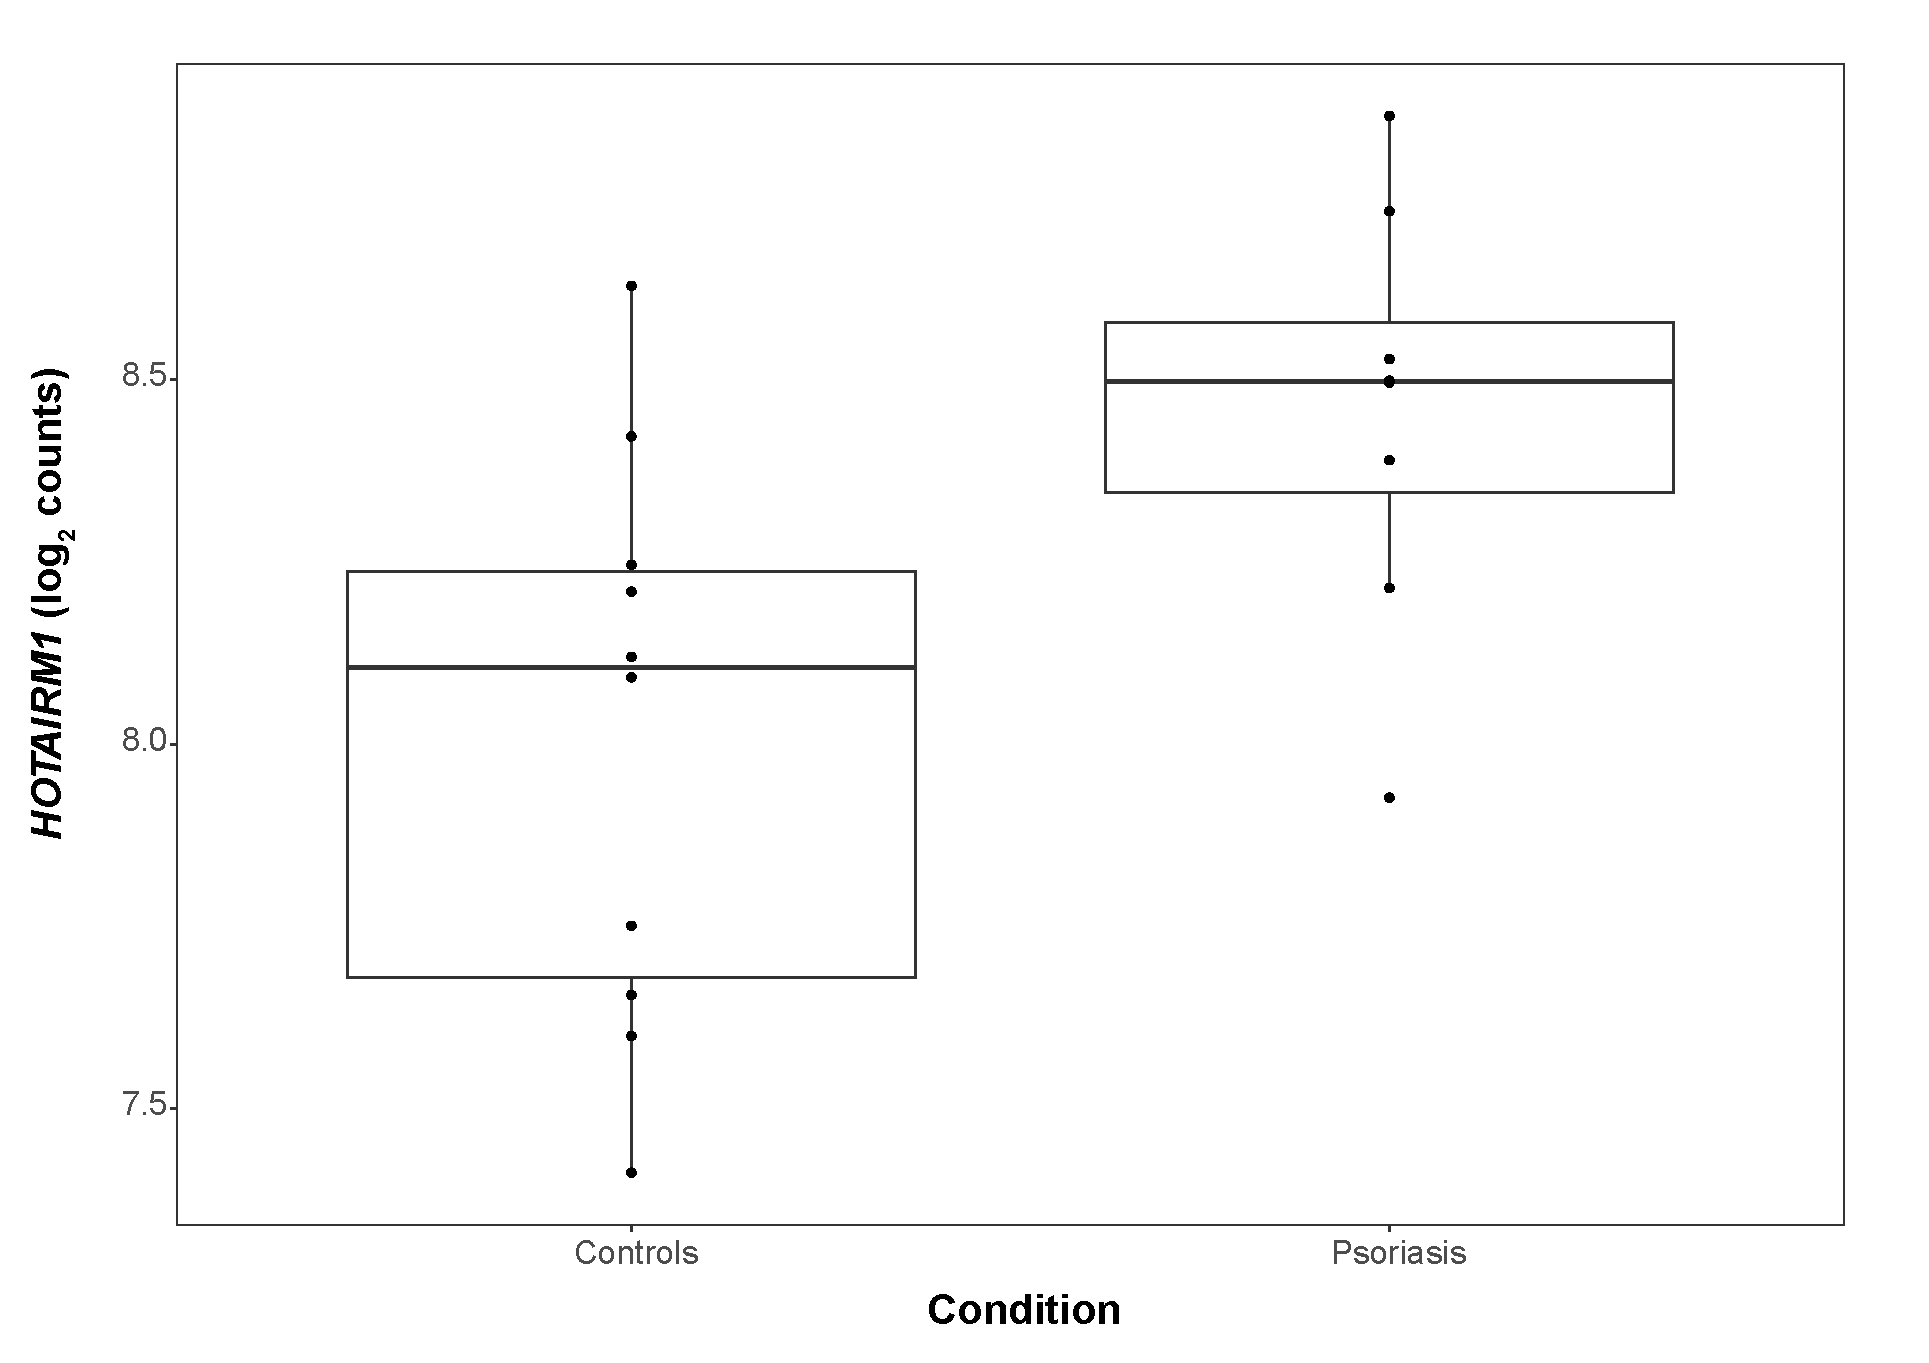
\includegraphics[width=\textwidth]{./Results2/pdfs/RNAseq_PS_CTL_lncRNA_HOTAIRM1_CD14}
\caption{\textbf{}}
% The percentage sign indicated that the other subfig goes side by side
\end{subfigure}%
\begin{subfigure}{0.45\textwidth}
\centering
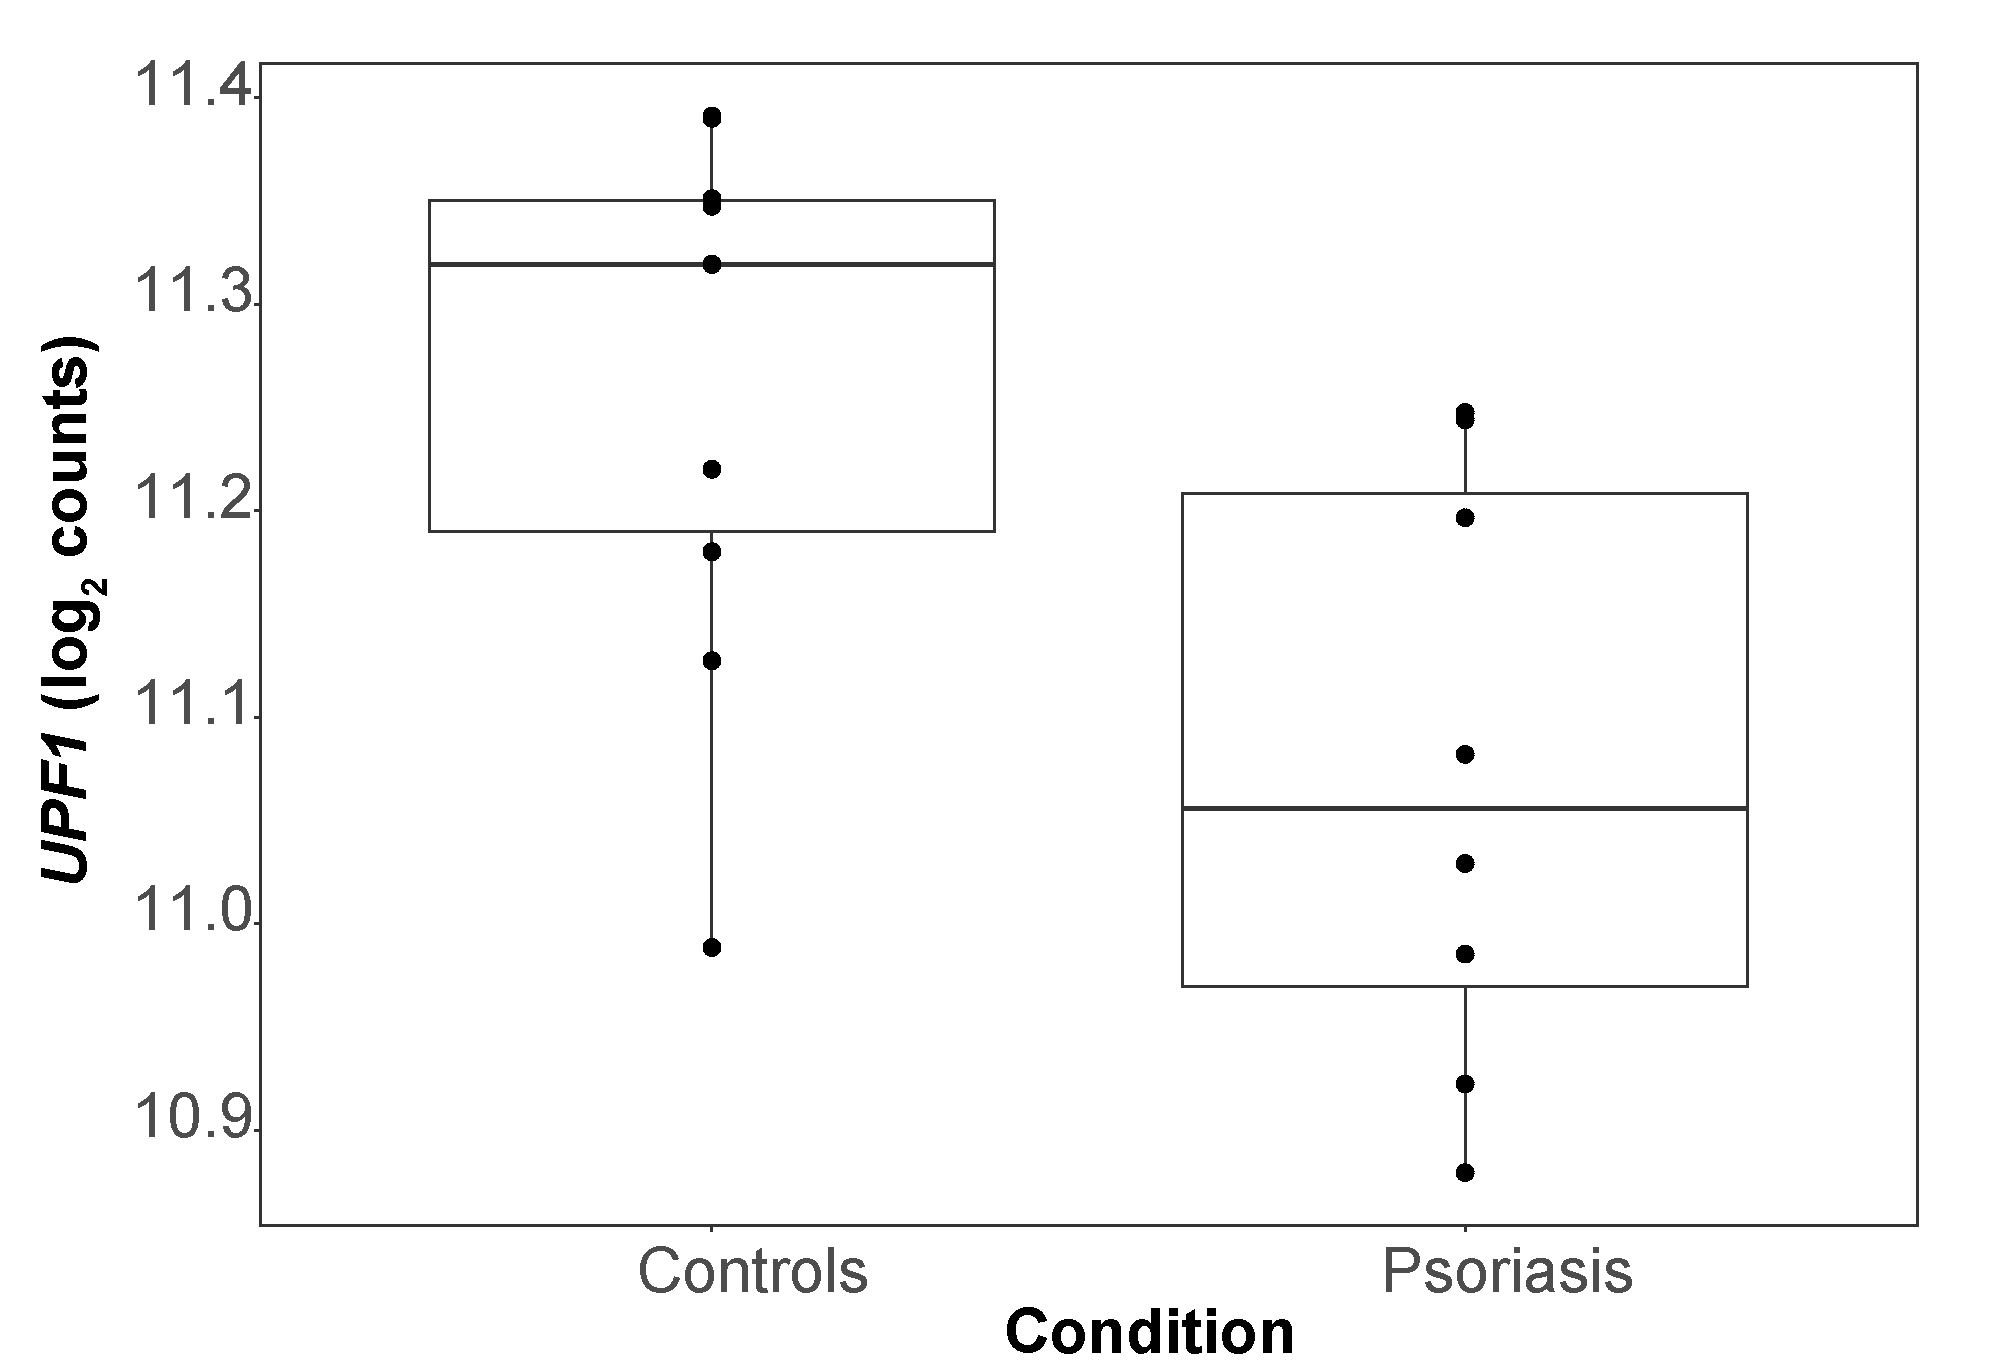
\includegraphics[width=\textwidth]{./Results2/pdfs/RNAseq_PS_CTL_lncRNA_UPF1_CD14}
\caption{\textbf{}}
\end{subfigure}
\caption[RNA-seq expression levels of the lncRNA \textit{HOTAIRM1} and its experimentally validated target \textit{UPF1} in psoriasis and healthy controls CD14$^+$ monocytes.]{\textbf{RNA-seq expression levels of the lncRNA \textit{HOTAIRM1} and its experimentally validated target \textit{UPF1} in psoriasis and healthy controls CD14$^+$ monocytes.} Expression is illustrated as the log$_2$ of the normalised read counts mapping to (A) the lncRNA \textit{HOTAIRM1} and (B) \textit{UPF1}, which has been experimentally identified as one of the genes regulated by this lncRNA according to NPInter database.}
\label{figure:RNAseq_PS_CTL_CD14_expression_HOTAIRM_UPF1}
\end{figure} 


The miR \textit{MIR146A} was the most relevant non-coding RNA dysregulated in CD8$^+$ T cells. \textit{MIR146A} showed down-regulation (fold change=0.73) in CD8$^+$ cells from psoriasis patients when compared to controls and has been shown previously to have a role in negative regulation of the innate immunity, inflammatory response and antiviral pathways \parencite{Taganov2006}.
%and was found to be down-regulated in psoriasis patients when compared to controls. %Molecular studies have suggested a role for miR-146a as a negative regulator of the TLR-4 pathway \parencite{Taganov2006}. 
%Other lncRNAs were found to be dysregulated in more than one cell type. For example, \textit{KCNQ1OT1} was downregulated in both, CD4$^+$ and CD8$^+$ cells. Dysregulated expression of this lncRNA has been reported in Beckwith-Wiedemann syndrome consisting of a loss-of-imprinting paediatric overgrowth disorder with some skin features such as creases or pits in the skin near the ears \parencite{Pandei2008}.


%This is in line with findings in serum from SLE and early RA patients \parencite{Wang2012,Filkova}. In contrast, trancriptomic studies using PBMCs from plaque psoriasis and also similar studies in RA (including PBMCs, SFMCs and CD4$^+$ isolated from both tissues, amongst others) have reported increased levels of miR-146a in patients when compared to controls \parencite{Ele-Refaei2015,Churov2015}. Molecular studies have suggested a role for miR-146a as a negative regulator of the TLR-4 pathway \parencite{Taganov2006}. This study demonstrated regulation of \textit{MIR146A} expression by NF-$\kappa$B upon inflammation as well as \textit{in vitro} targeting of the 3'UTR of \textit{TRAF6} and IL-1 receptor-associated kinase 1 (\textit{IRAK1}) genes. These are adaptor molecules that lead to activation of kinases from the TLR-4 pathway that eventually lead to translocation of NF-$\kappa$B and AP-1 into the nucleus and transcriptional up-regulation of inflammatory genes. 

%Other lncRNAs were found to be dysregulated in more than one cell type. For example, \textit{KCNQ1OT1} was downregulated in both, CD4$^+$ and CD8$^+$ cells. Dysregulated expression of this lncRNA has been reported in Beckwith-Wiedemann syndrome consisting of a loss-of-imprinting paediatric overgrowth disorder with some skin features such as creases or pits in the skin near the ears \parencite{Pandei2008}. \textit{KCNQ1OT1} has been reported to interact with DNA methyltransferases and also to facilitate the interaction of these enzymes with the chromatin, leading to misregulation of imprinted loci.



\subsubsection{Pathway enrichment analysis}

To investigate the biological role of the differences in gene expression between psoriasis patients and healthy controls, pathway enrichment analysis was performed for each cell type using DEG with FDR$<$0.05 and no fold change cut-off. This analysis revealed biologically relevant pathways significantly enriched (FDR$<$0.01) for DEGs in CD14$^+$ monocytes and CD8$^+$ cells (Table \ref{tab:RNAseq_PS_CTL_pathway_enrichment} and \ref{tab:RNAseq_PS_CTL_additional_pathways}). In CD19$^+$ cells, only one pathway (“generic transcription”, p-value=8.2x10$^{-12}$, fold change=6.26) showed significant enrichment, whereas in CD4$^+$ cells no enrichment was seen for any pathway. 


%The moderated fold changes in the DGE analysis illustrated in the volcano plots suggest that the differences between patients and controls in these circulating immune cells are discrete. Nevertheless, moderate differences may have an important impact on their phenotype for infiltration and activation in the skin. Therefore, exploratory pathway analysis was conducted using DEG with FDR$<$0.05 and no fold change cut off. Biologically relevant pathways appeared to be significantly enriched (FDR$<$0.01) for CD14$^+$ monocytes and CD8$^+$ cells DEGs (Table \ref{tab:tab:RNAseq_PS_CTL_pathway_enrichment} and \ref{tab:RNAseq_PS_CTL_additional_pathways}). In CD19$^+$ cells, only one pathway (“generic transcription”) appeared to be significantly enriched for DEGs in this cell type. In contrast, in CD4$^+$ cells modulated genes between psoriasis patients and controls were not enriched for any pathway. 

MAPK signalling and IL-12 mediated signalling pathways were enriched in both, CD14$^+$ monocytes and CD8$^+$ cells (Table \ref{tab:RNAseq_PS_CTL_pathway_enrichment}). MAPK signalling was of particular interest as DEGs contributing to this enrichment included a number of MAPK genes that were differentially expressed between psoriasis patients and healthy controls (Figure \ref{figure:RNAseq_PS_CTL_MAPK_and_DUSP_genes_boxplots}). Two of those MAPK genes, \textit{MAP3K4} and \textit{MAPK14}, were down-regulated in psoriasis compared to controls in CD14$^+$ monocytes and CD8$^+$ T cells (Figure \ref{figure:RNAseq_PS_CTL_MAPK_and_DUSP_genes_boxplots}A and B). MAP3K4 is a member of the MAPKKK family, whose expression is down-regulated in LPS-stimulated PBMCs from CD patients leading to a relative immune deficiency in TLR-mediated cytokine production.

\begin{table}[htbp]
%\setlength{\tabcolsep}{20pt} only to stretch the columns if you want
\renewcommand{\arraystretch}{0.8}
\centering
\begin{tabular}{@{} c c c c}
\toprule
\textbf{Cell type}     & \textbf{Pathways}                   & \textbf{FDR} &  \textbf{Fold change} \\
\midrule
\midrule
                      & MAPK signalling                      &3.4x10$^{-5}$  &  2.83 \\
											
                      & IL-12 mediated signaling events      &6.2x10$^{-6}$  &  4.82 \\
				              & Th-1 and Th-2 cell differentiation   &2.4x10$^{-4}$  &  3.34  \\
CD14$^+$              & Th-17 cell differentiation           &2.4x10$^{-4}$  &  3.21 \\
				              & TCR signalling                       &5.3x10$^{-5}$  &  3.18 \\
				              & Platelet-derived growth factor (PDGF-$\beta$) & 1.8x10$^{-3}$& 2.59 \\
				              & Forkhead box O (FoxO) signalling     &3.6x10$^{-3}$  &  2.38 \\
\midrule				
                      & Osteoclast differentiation           &7.2x10$^{-5}$  &3.45  \\
                      & MAPK signalling                      &1.5x10$^{-3}$  &2.33 \\
				              & TNF signalling                       &1.5x10$^{-3}$  &2.93 \\
CD8$^+$               & IL-12 mediated signalling events     &5.5x10$^{-4}$  &3.86 \\
				              & NF-$\kappa$B signalling              &2.2x10$^{-3}$  &2.95 \\
				              & Chemokine signalling                 &2.3x10$^{-3}$  &2.43  \\
\bottomrule
\end{tabular}
\medskip %gap
\caption[Pathways enriched for DEGs between psoriasis patients and healthy controls in CD14$^+$ monocytes and CD8$^+$ cells.]{\textbf{Pathways enriched for DEGs between psoriasis patients and healthy controls in CD14$^+$ monocytes and CD8$^+$ cells.} The enrichment analysis was conducted using significant DEGs (FDR$<$0.05) and no fold change threshold. Significant enriched pathways (FDR$<$0.01) had a minimum of ten members overlapping DEGs in the corresponding cell type.}
\label{tab:RNAseq_PS_CTL_pathway_enrichment}
\end{table}


Moreover, differential gene expression analysis of members of the dual-specificity phosphatases (DUSP) family, involved in fine-tuning of the immune response \parencite{Qian2009}, also contributed to the enrichment of the MAPK pathway in both cell types. \textit{DUSP10} was down-regulated (fold change=0.83) in psoriasis CD14$^+$ monocytes (Figure \ref{figure:RNAseq_PS_CTL_MAPK_and_DUSP_genes_boxplots}C) and the knock-out of this gene in mice has been shown to enhanced inflammation \parencite{Qian2009}. Conversely, \textit{DUSP4} was up-regulated (fold change=1.47) in psoriasis CD8$^+$ cells compared to healthy controls (Figure \ref{figure:RNAseq_PS_CTL_MAPK_and_DUSP_genes_boxplots}D) and has been demonstrated to have a pro-inflammatory role in a sepsis mice model \parencite{Cornell2010}.


\begin{figure}[htbp]
\centering
\begin{subfigure}{0.5\textwidth}
\centering
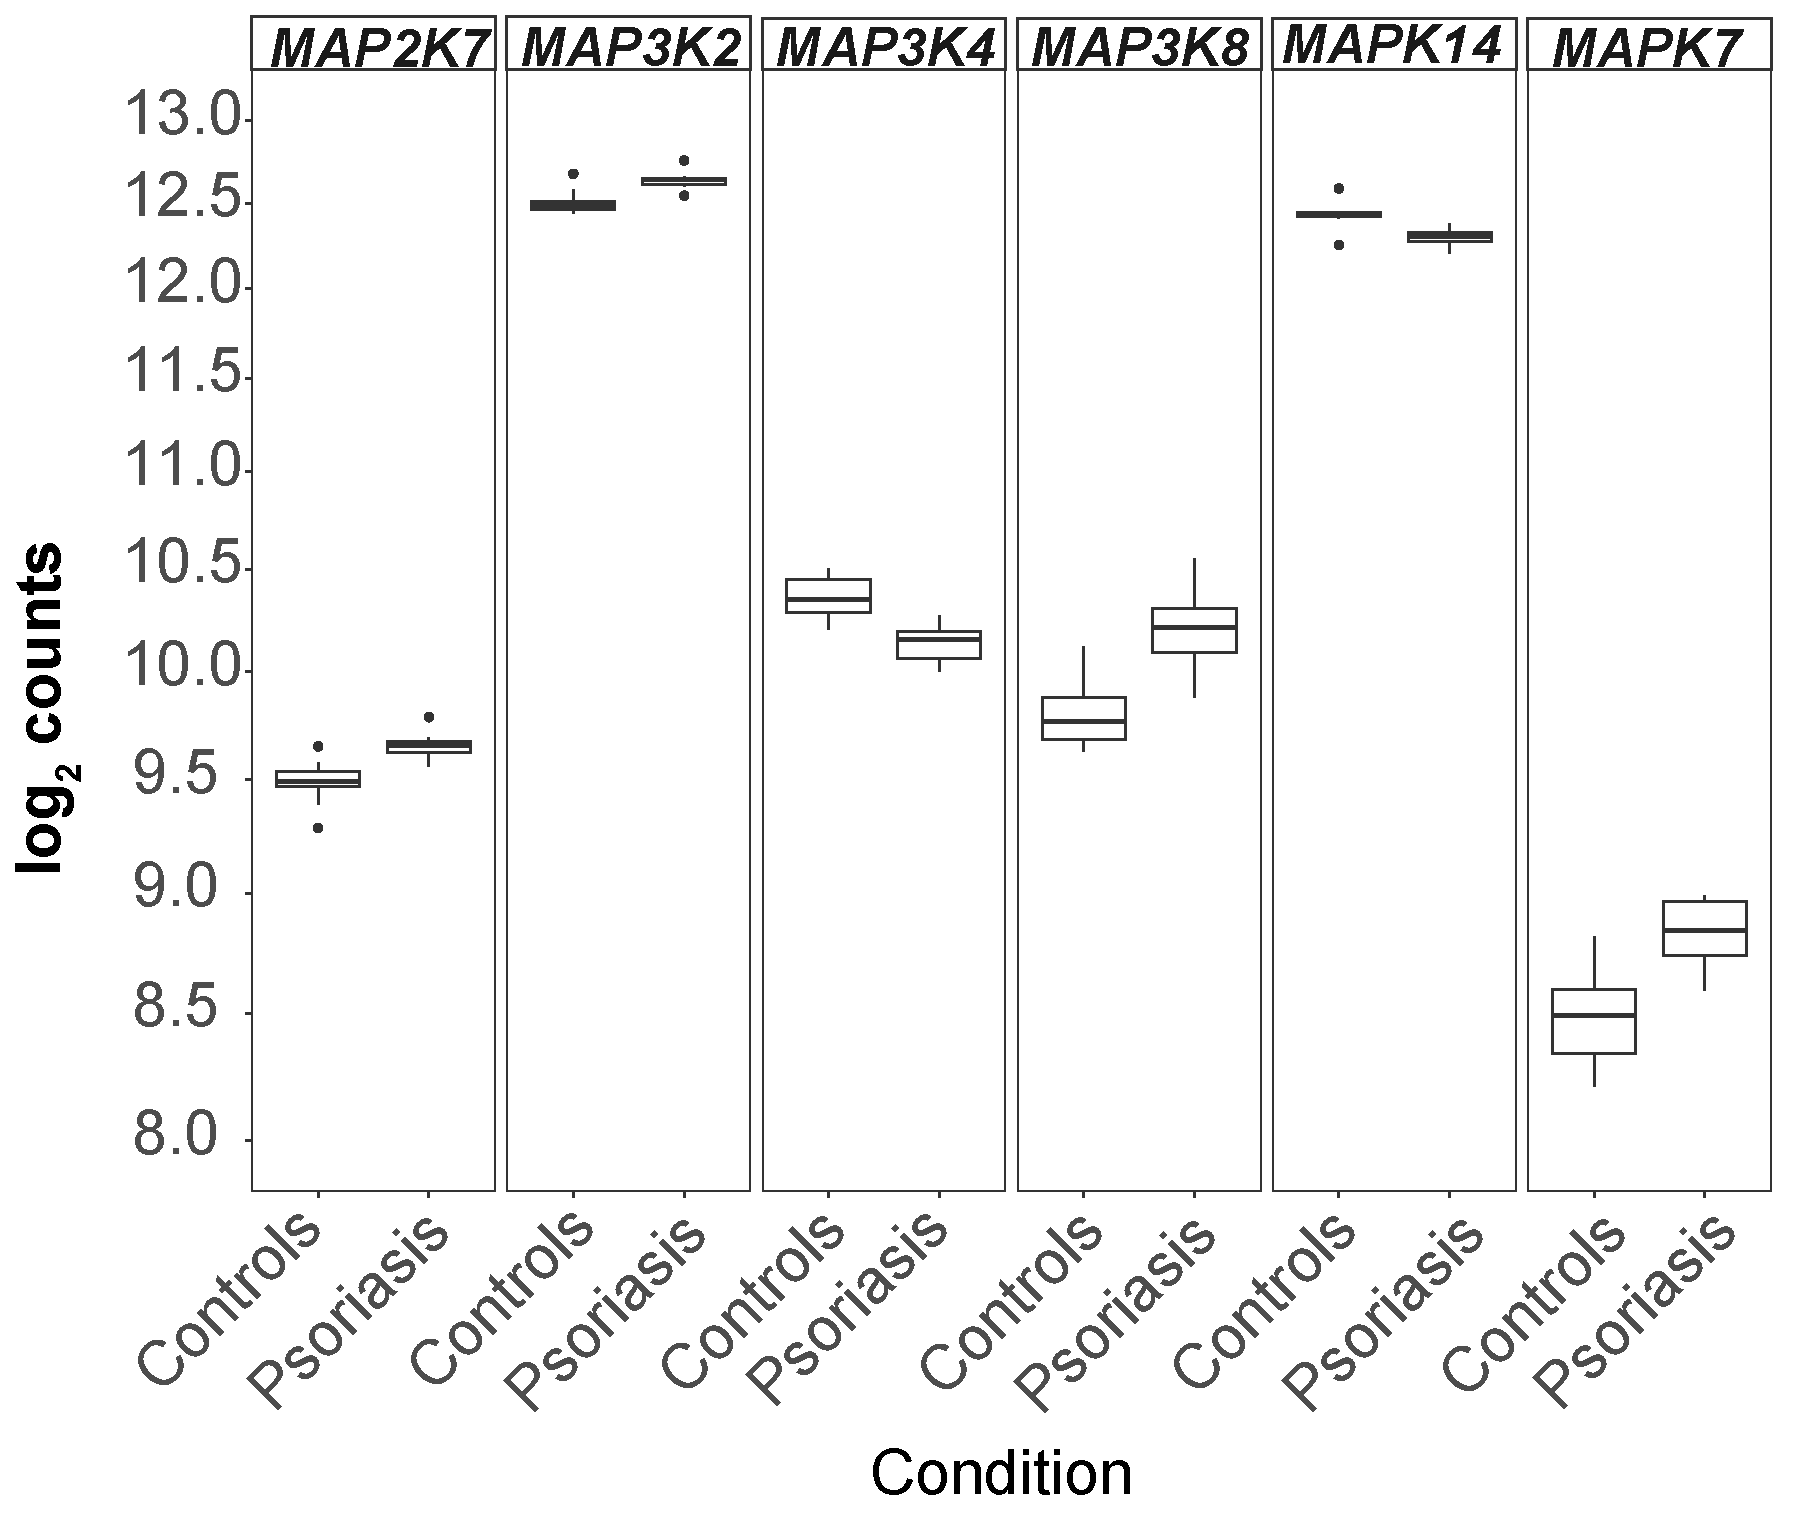
\includegraphics[width=\textwidth]{./Results2/pdfs/RNAseq_PS_CTL_CD14_MAPK_boxplots}
\caption{\textbf{}}
% The percentage sign indicated that the other subfig goes side by side
\end{subfigure}
\begin{subfigure}{0.5\textwidth}
\centering
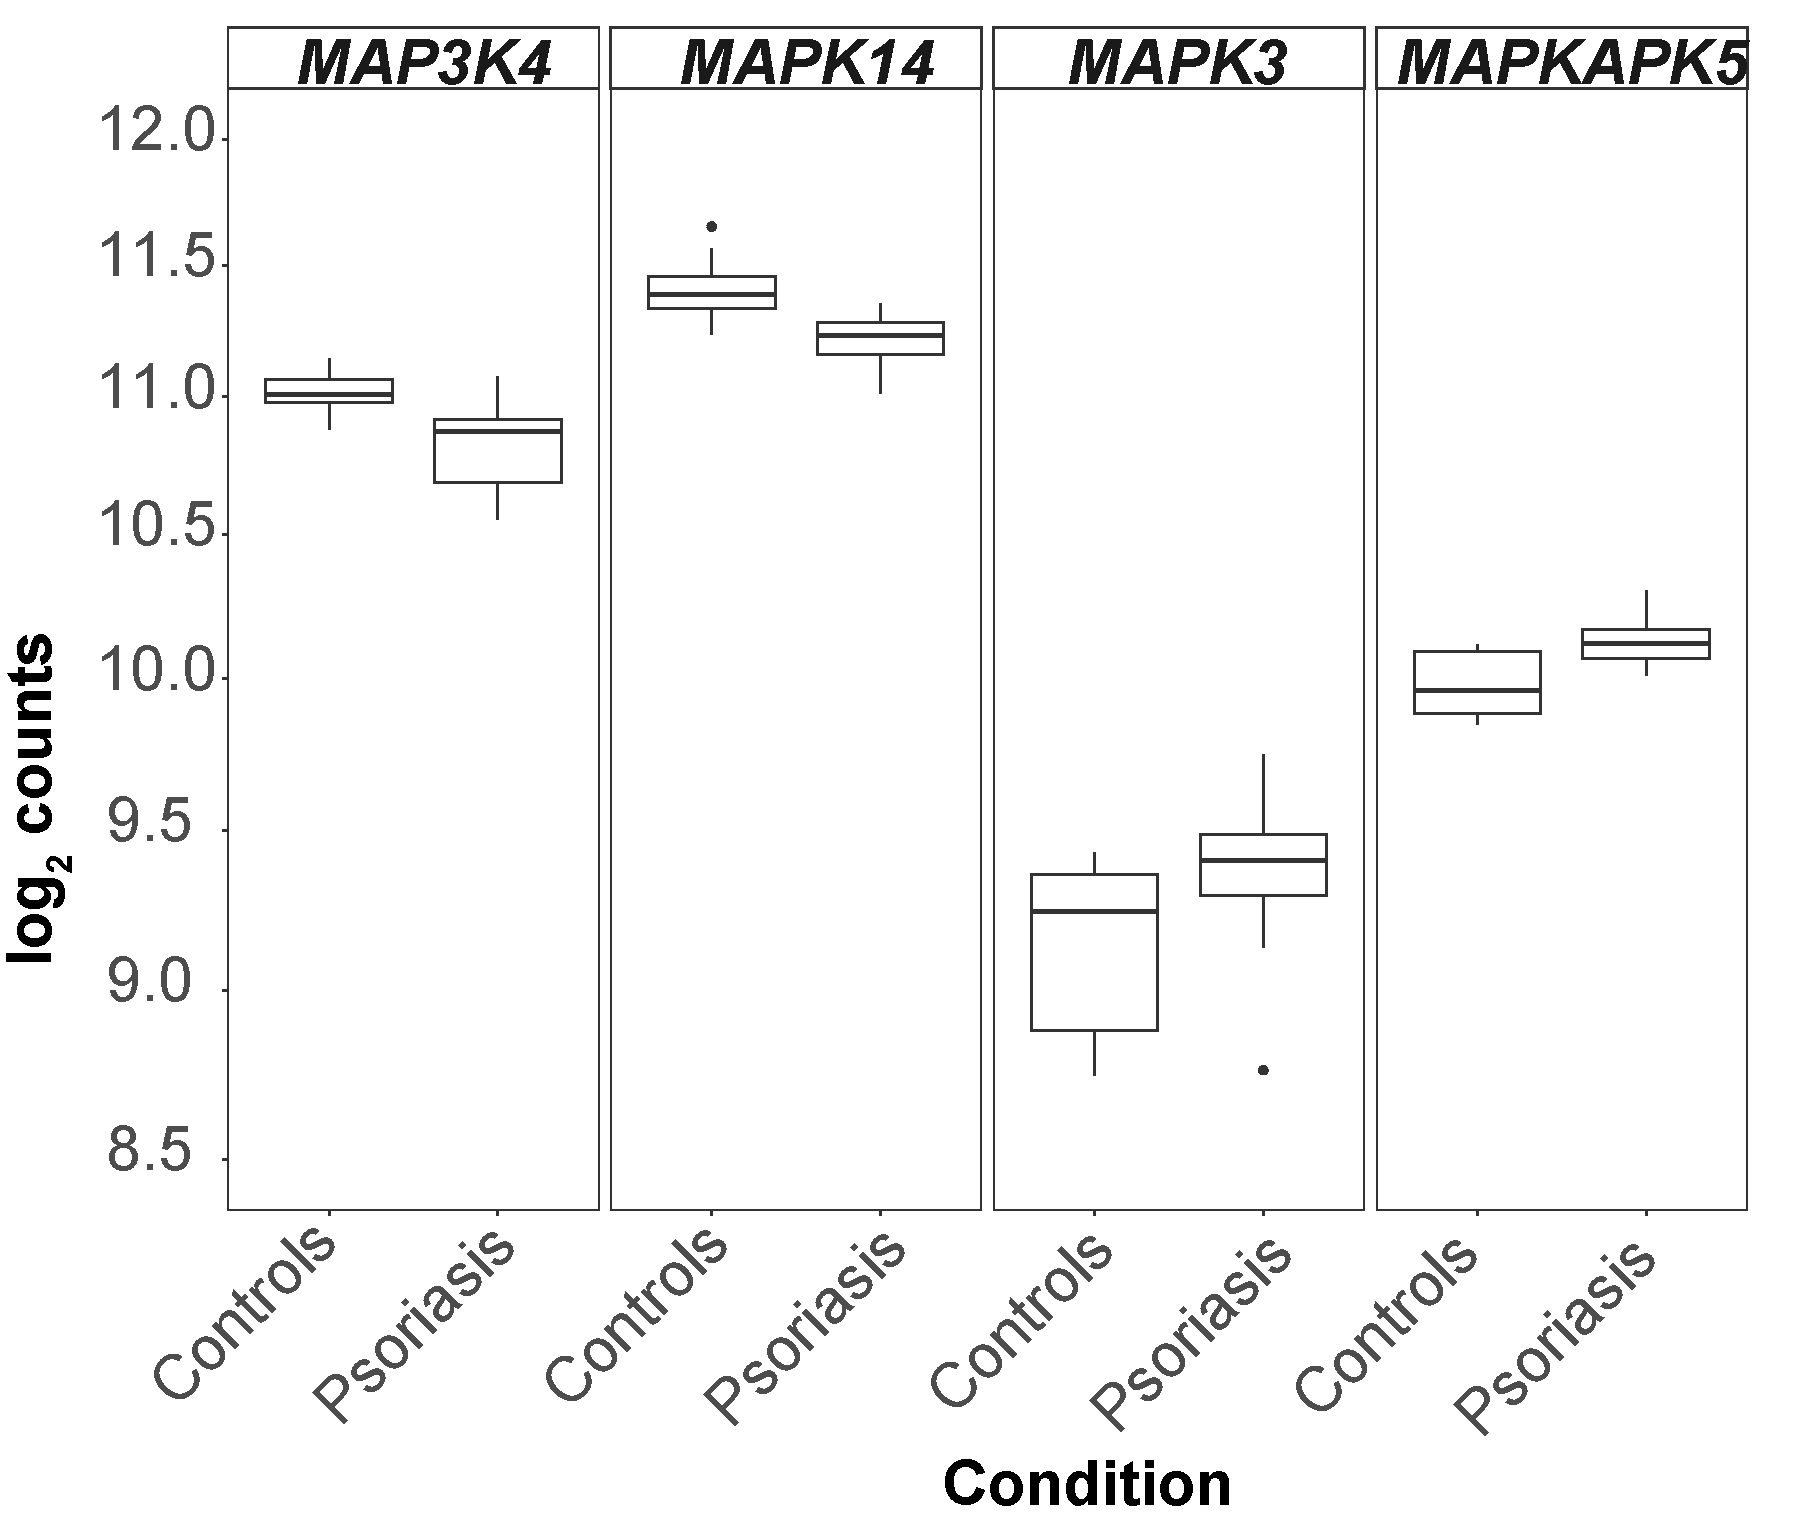
\includegraphics[width=\textwidth]{./Results2/pdfs/RNAseq_PS_CTL_CD8_MAPK_boxplots}
\caption{\textbf{}}
\end{subfigure}
\begin{subfigure}{0.45\textwidth}
\centering
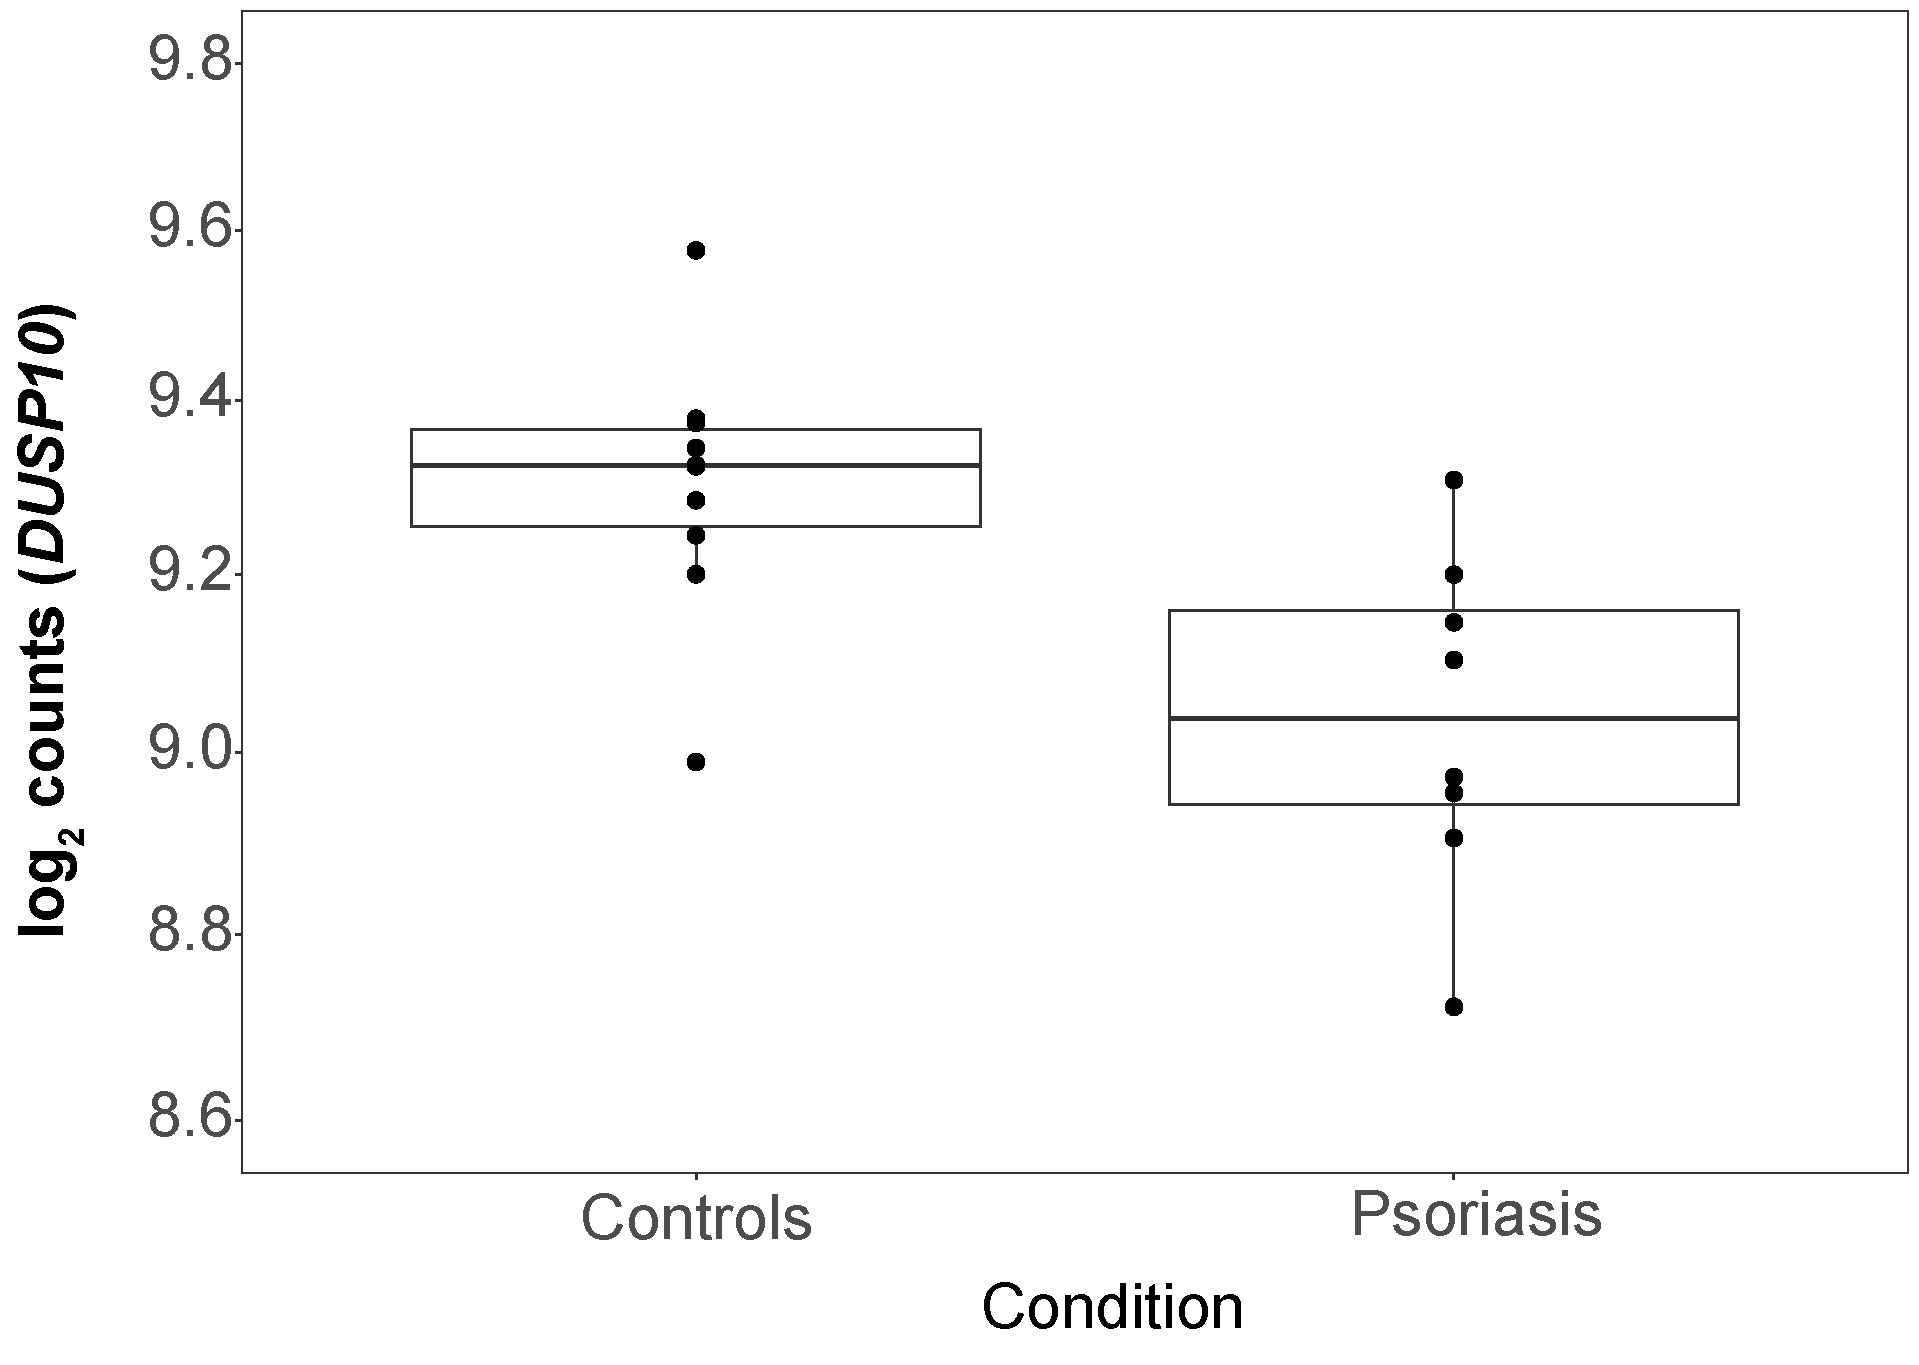
\includegraphics[width=\textwidth]{./Results2/pdfs/RNAseq_PS_CTL_CD14_DUSP10_boxplot}
\caption{\textbf{}}
% The percentage sign indicated that the other subfig goes side by side
\end{subfigure}%
\begin{subfigure}{0.45\textwidth}
\centering
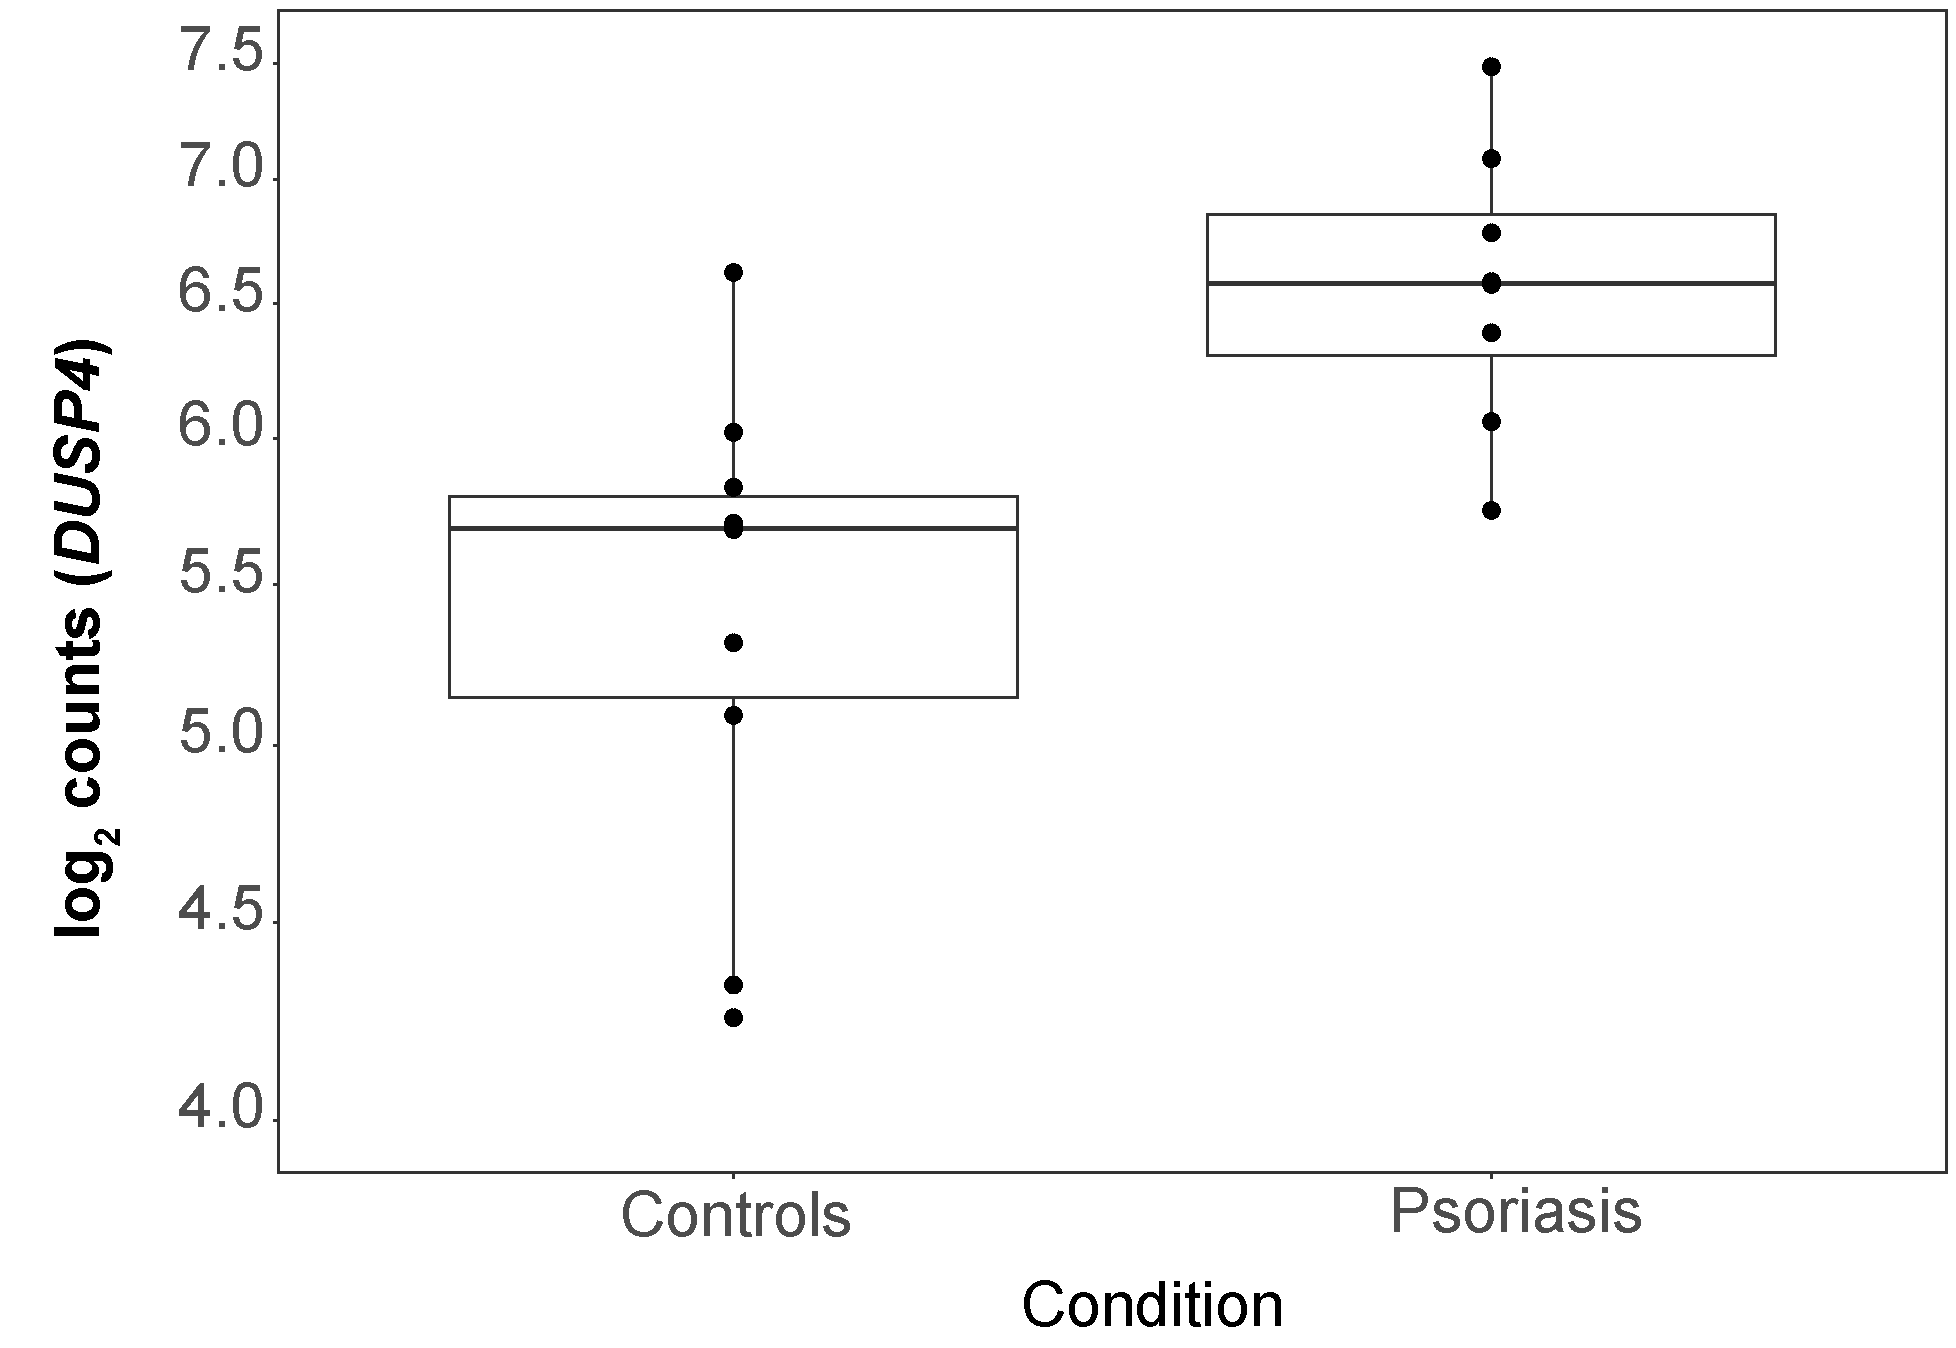
\includegraphics[width=\textwidth]{./Results2/pdfs/RNAseq_PS_CTL_CD8_DUSP4_boxplot}
\caption{\textbf{}}
\end{subfigure}
\caption[Differential expression between psoriasis and healthy controls of \textit{MAPK} and \textit{DUSP} genes contributing to MAPK signalling enrichment in CD14$^+$ monocytes and CD8$^+$ T cells.]{\textbf{Differential expression between psoriasis and healthy controls of \textit{MAPK} and \textit{DUSP} genes contributing to MAPK signalling enrichment in CD14$^+$ monocytes and CD8$^+$ T cells.} Expression for MAPK genes in psoriasis patients and controls is illustrated as the log$_2$ of the normalised read counts, including (A) \textit{MAP2K7}, \textit{MAP3K2}, \textit{MAP3K4}, \textit{MAP3K8}, \textit{MAPK14} and \textit{MAPK7} in CD14$^+$ monocytes and (B) \textit{MAP3K4}, \textit{MAPK14}, \textit{MAPK3} and \textit{MAPKAPK5} in CD8$^+$ T cells. Similarly, expression as log$_2$ of the normalised read counts is also illustrated for the DUSP gene members (C) \textit{DUSP10} in CD14$^+$ monocytes and (D) \textit{DUSP4} in CD8$^+$ T cells, in patients and control samples.}
\label{figure:RNAseq_PS_CTL_MAPK_and_DUSP_genes_boxplots}
\end{figure} 

%Enrichment was shared between CD14$^+$ monocytes and CD8$^+$ cells. Some of the DEGs contributing to the enrichment of this pathway in both cell types included MAPK gene members such as \textit{MAP3K4} and \textit{MAPK14}, both down-regulated in psoriasis when compared to controls. Interestingly, MAP3K4 is a member of the MAPKKK family, for which expression is down-regulated in LPS-stimulated PBMCs from CD patients, leading to reduced expression of the cytokine \textit{IL-1A} and a relative immune deficiency in TLR-mediated cytokine production. Moreover, DGE of members of the dual-specificity phosphatases (DUSP) family involved in fine-tuning the immune response \parencite{Qian2009} contribute to the enrichment of the MAPK pathway in CD14$^+$ monocytes and CD8$^+$ cells. \textit{DUSP10} was down-regulated in the psoriasis CD14$^+$ monocytes and could be modulating reactive oxygen species production according to a knock-out mice phenotype presenting enhanced inflammation \parencite{Qian2009}. Conversely, \textit{DUSP4} presented up-regulation in CD8$^+$ patients when compared to healthy controls and it could represent a pro-inflammatory feature as this gene has been demonstrated to have a role in driving inflammation in a sepsis mice model \parencite{Cornell2010}.  

Amongst members of the enriched IL-12 signalling pathway, \textit{STAT4} and \textit{STAT5A} were down-regulated (fold change 0.82 and 0.90, respectively) in CD14$^+$ monocytes from psoriasis patients. Neither \textit{STAT4} or \textit{STAT5A} were differentially expressed in CD8$^+$ cells. In contrast, \textit{IFNG} expression in psoriasis patients was lower than in healthy controls CD8$^+$ cells (fold change=0.66), showing no differences in CD14$^+$ monocytes. Also, \textit{IL2RA} only demonstrated up-regulation (fold change=1.36) in CD8$^+$ T cells and this may have an effect in the formation of the receptor IL2-R$\alpha$ and consequently on IL-2 signalling, which is involved in effector and Treg cell differentiation \parencite{Malek2010}.

Pathways only enriched for CD14$^+$ monocytes DEGs platelet-derived growth factor (PDGF-$\beta$) signalling, and unexpectedly T cell related pathways such as TCR signalling and Th17 cell differentiation (Table \ref{tab:RNAseq_PS_CTL_pathway_enrichment}). Dysregulated genes involved in the PDGF-$\beta$ signalling included the down-regulation (fold change=0.84) in psoriasis samples of the \textit{SLA}, for which a knock-out mice model has shown impaired IL-12 and TNF-$\alpha$ production and failure of T cell stimulation by GM-CSF treated bone marrow-derived DCs \parencite{Liontos2011}.

%Other interesting pathways enriched for both cell types  included IL-12 mediated signalling (Table \ref{tab:RNAseq_PS_CTL_pathway_enrichment}). IL-12 signalling leads to T cell proliferation and IFN-$\gamma$ production through activation of TFs from the STAT family. Importantly STAT4 is a well-known drug target for psoriasis treatment. Interestingly, CD14$^+$ monocytes from psoriasis presented down-regulation of \textit{STAT4} and \textit{STAT5A} in patients compared to controls. Likewise, \textit{IFNG} expression in psoriasis patients was lower than in healthy controls in CD8$^+$ cells. This phenomenon has been previously observed in macrophages derived from AS patients as well as in an SpA rat model \parencite{Smith2008,Fert2014}. Additionally, \textit{IL2RA} was up-regulated in CD8$^+$ from psoriasis patients when compared to controls, which may enhance formation of the IL2-R$\alpha$ and the signalling by this cytokine involved in effector and regulatory T cell differentiation \parencite{Malek2010}.


Notably, a number of very relevant inflammatory pathways were enriched only for CD8$^+$ DEGs between psoriasis patients and controls. These included TNF, NF-$\kappa$B and chemokine signalling (Table \ref{tab:RNAseq_PS_CTL_pathway_enrichment}), with some of the DEGs contributing to more than one of the pathways. Enrichment of these three pathways resulted from combined up- and down-regulation of activators and inhibitors of the immune response. This included unexpected up-regulated in psoriasis CD8$^+$ T of the anti-inflammatory genes NF-$\kappa$B inhibitor A (\textit{NFKBIA}) and the TNF-$\alpha$ induced protein 3 (\textit{TNFAIP3}) (fold change 1.32 and 1.36, respectively), both involved in TNF and NF-$\kappa$B signalling (Figure \ref{figure:RNAseq_PS_CTL_CD8_TNF_and_chemokine_pathway_modified}A (green box) and B, in bold).  As previously mentioned, \textit{NFKBIA} and \textit{TNFAIP3} were also up-regulated in psoriasis CD14$^+$ monocytes and CD4$^+$ cells, respectively (Table \ref{tab:RNAseq_PS_CTL_GWAS_overlap}). Pro-inflammatory genes that showed down-regulation in psoriasis when compared to healthy controls included the activating transcription factor 2 (\textit{ATF2}) (Figure \ref{figure:RNAseq_PS_CTL_CD8_TNF_and_chemokine_pathway_modified}A, in bold) and the protein kinase C beta\textit{PRKCB} (Figure \ref{figure:RNAseq_PS_CTL_CD8_TNF_and_chemokine_pathway_modified}A (green box) and B, in bold). In contrast, \textit{ATF4}, JunB proto-oncogene (\textit{JUNB}) coding for one of the subunits of the TF AP-1 and three of the NF-$\kappa$B subunits including \textit{RELA}, \textit{RELB} and \textit{NFKB2} were amonsgt the pro-inflammatory genes up-regulated in psoriasis compared to controls (Figure \ref{figure:RNAseq_PS_CTL_CD8_TNF_and_chemokine_pathway_modified}A). Furthermore, enrichment of the chemokine signalling pathway involved up-regulation in psoriasis CD8$^+$ T cells of \textit{CCR10} (fold change=1.34), receptor for the chemotactic skin-associated chemokine CCL27, and \textit{CXCR4} (fold change=1.59), receptor for the chemokine CXCL12, highly expressed in skin \parencite{Zgraggen2014} (Figure \ref{figure:RNAseq_PS_CTL_CD8_TNF_and_chemokine_pathway_modified}B), which would facilitate T cell migration into the affected epidermis. In contrast,  \textit{CXCR1} and \textit{CX3CR1} , receptors of IL8 and CX3CL1 respectively, were down-regulated in psoriais compared to healthy controls. Notably, none of the chemokines showed differential expression in this analysis (Figure \ref{figure:RNAseq_PS_CTL_CD8_TNF_and_chemokine_pathway_modified}B, not in bold). 
	
These data highlight the dysregulation in CD14$^+$ monocytes and CD8$^+$ T cells of relevant pathways in psoriasis pathophysiology resulting from combined up- and down-regulation of pro- and anti-inflammatory genes which difficults the interpretation of the overall effect of those interactions in the inflammatory response.


%Genes such as the activating transcription factor 2 (\textit{ATF2}) and 4 (\textit{ATF4}) members of the TNF signalling cascade and the protein kinase C beta\textit{PRKCB} from the NF-$\kappa$B and chemokine signalling pathways appeared down-regulated in psoriasis vs healthy controls. In contrast, JunB proto-oncogene (\textit{JUNB}) coding for one of the subunits of the TF AP-1 and three of the NF-$\kappa$B subunits including \textit{RELA}, \textit{RELB} and \textit{NFKB2} showed up-regulation in patients vs controls. Particularly, AP-1, undergoes activation following growth factors, cytokines, chemokines, hormones and multiple environmental stresses and acts as a negative regulator of cell proliferation and IL-6 production \parencite{Schonthaler2011}.

%Genes with prominent pro-inflammatory role in the NF-$\kappa$B or TNF signalling pathways also appeared to be down-regulated, such as the activating transcription factor 2 (\textit{ATF2}) and 4 (\textit{ATF4}) members of the TNF signalling cascade and the protein kinase C beta\textit{PRKCB} from the NF-$\kappa$B and chemokine signalling pathways. Up-regulation of pro-inflammatory genes JunB proto-oncogene (\textit{JUNB}) coding for one of the subunits of the TF AP-1 and three of the NF-$\kappa$B subunits including \textit{RELA}, \textit{RELB} and \textit{NFKB2}. 


%Interestingly, \textit{NFKBIA} and \textit{TNFAIP3} were also up-regulated in CD14$^+$ monocytes and CD4$^+$ cells. \textit{NFKBIA} codes for the NF-$\kappa$B inhibitor alpha (I$\kappa$B$\alpha$) which binds to the NF-$\kappa$B subunits preventing them from translocation to the nucleus by masking a nuclear localisation signal (NLS). Similarly, \textit{TNFAIP3} codes for the zinc finger protein and ubiqitin-editing enzyme A20, that inhibits both NF-$\kappa$B signalling and TNF-mediated apoptosis. Unexpectedly, these two genes with an anti-inflammatory role appeared to be up-regulated in psoriasis patients when compared to controls in two of the studied cell types. 


\begin{figure}[htbp]
\centering
\begin{subfigure}{0.8\textwidth}
\centering
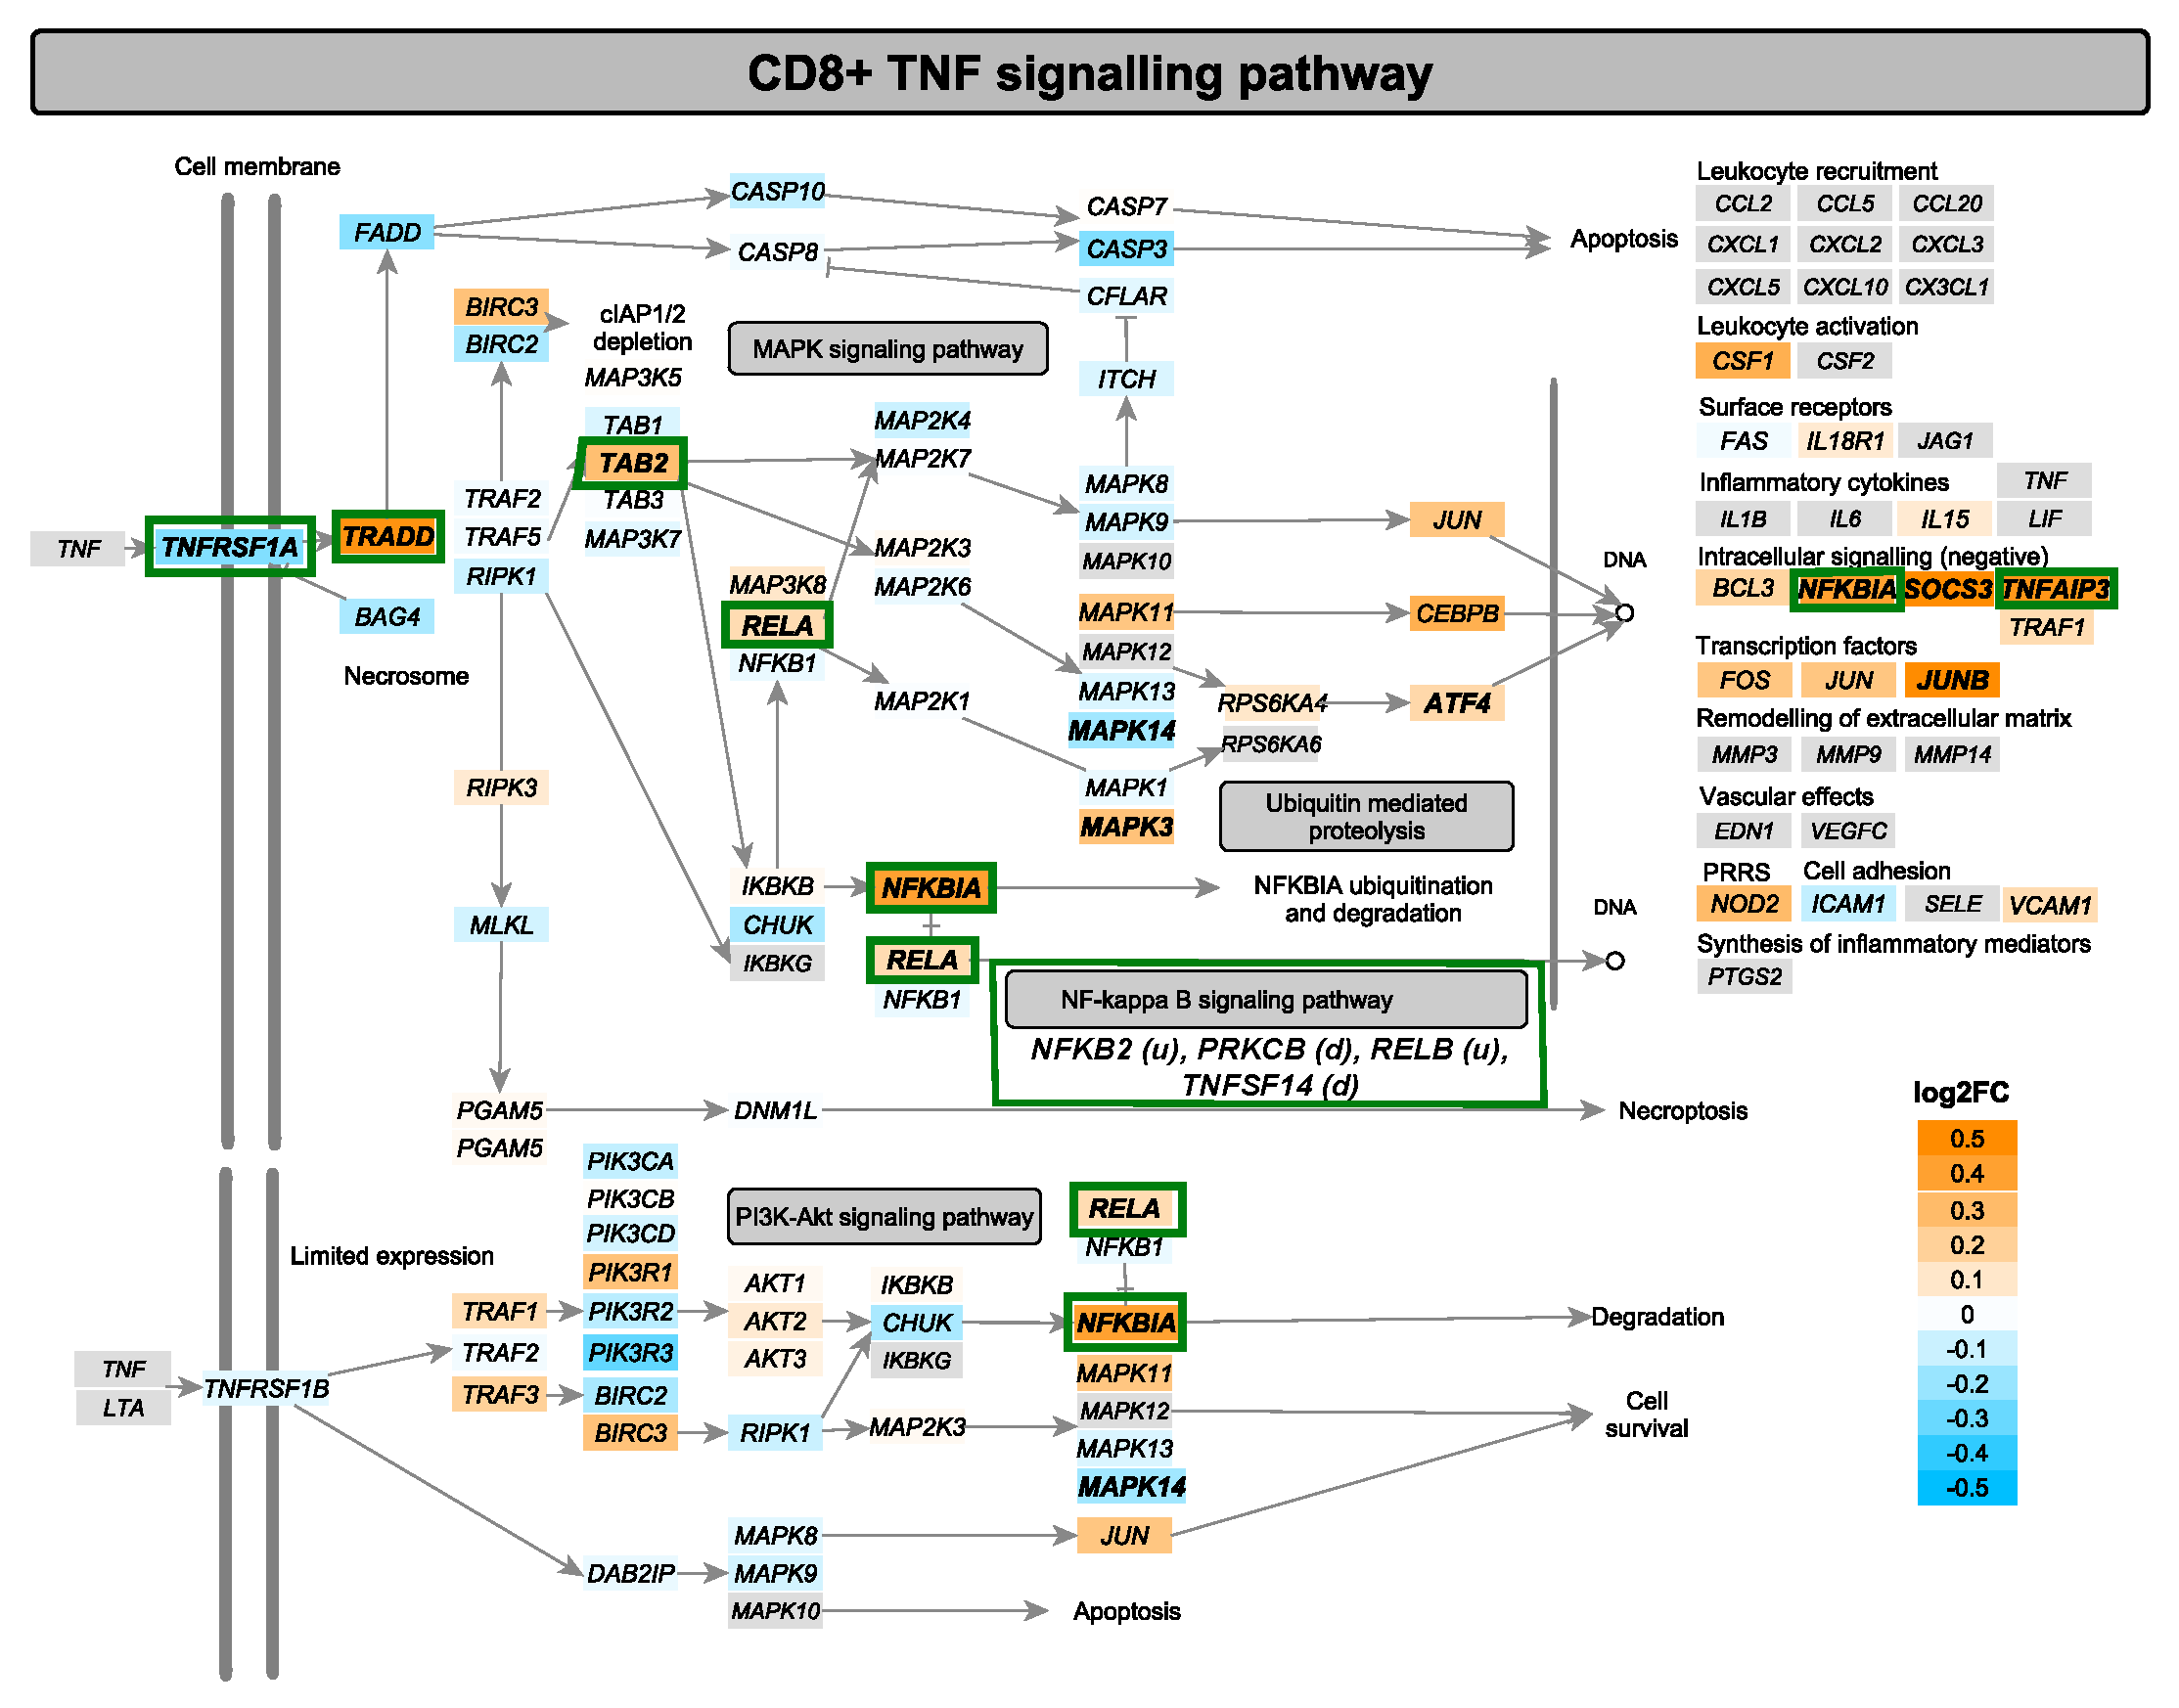
\includegraphics[width=\textwidth]{./Results2/pdfs/PS_CTL_CD8_all_TNF_pathway}
\caption{\textbf{}}
% The percentage sign indicated that the other subfig goes side by side
\end{subfigure}
\begin{subfigure}{0.8 \textwidth}
\centering
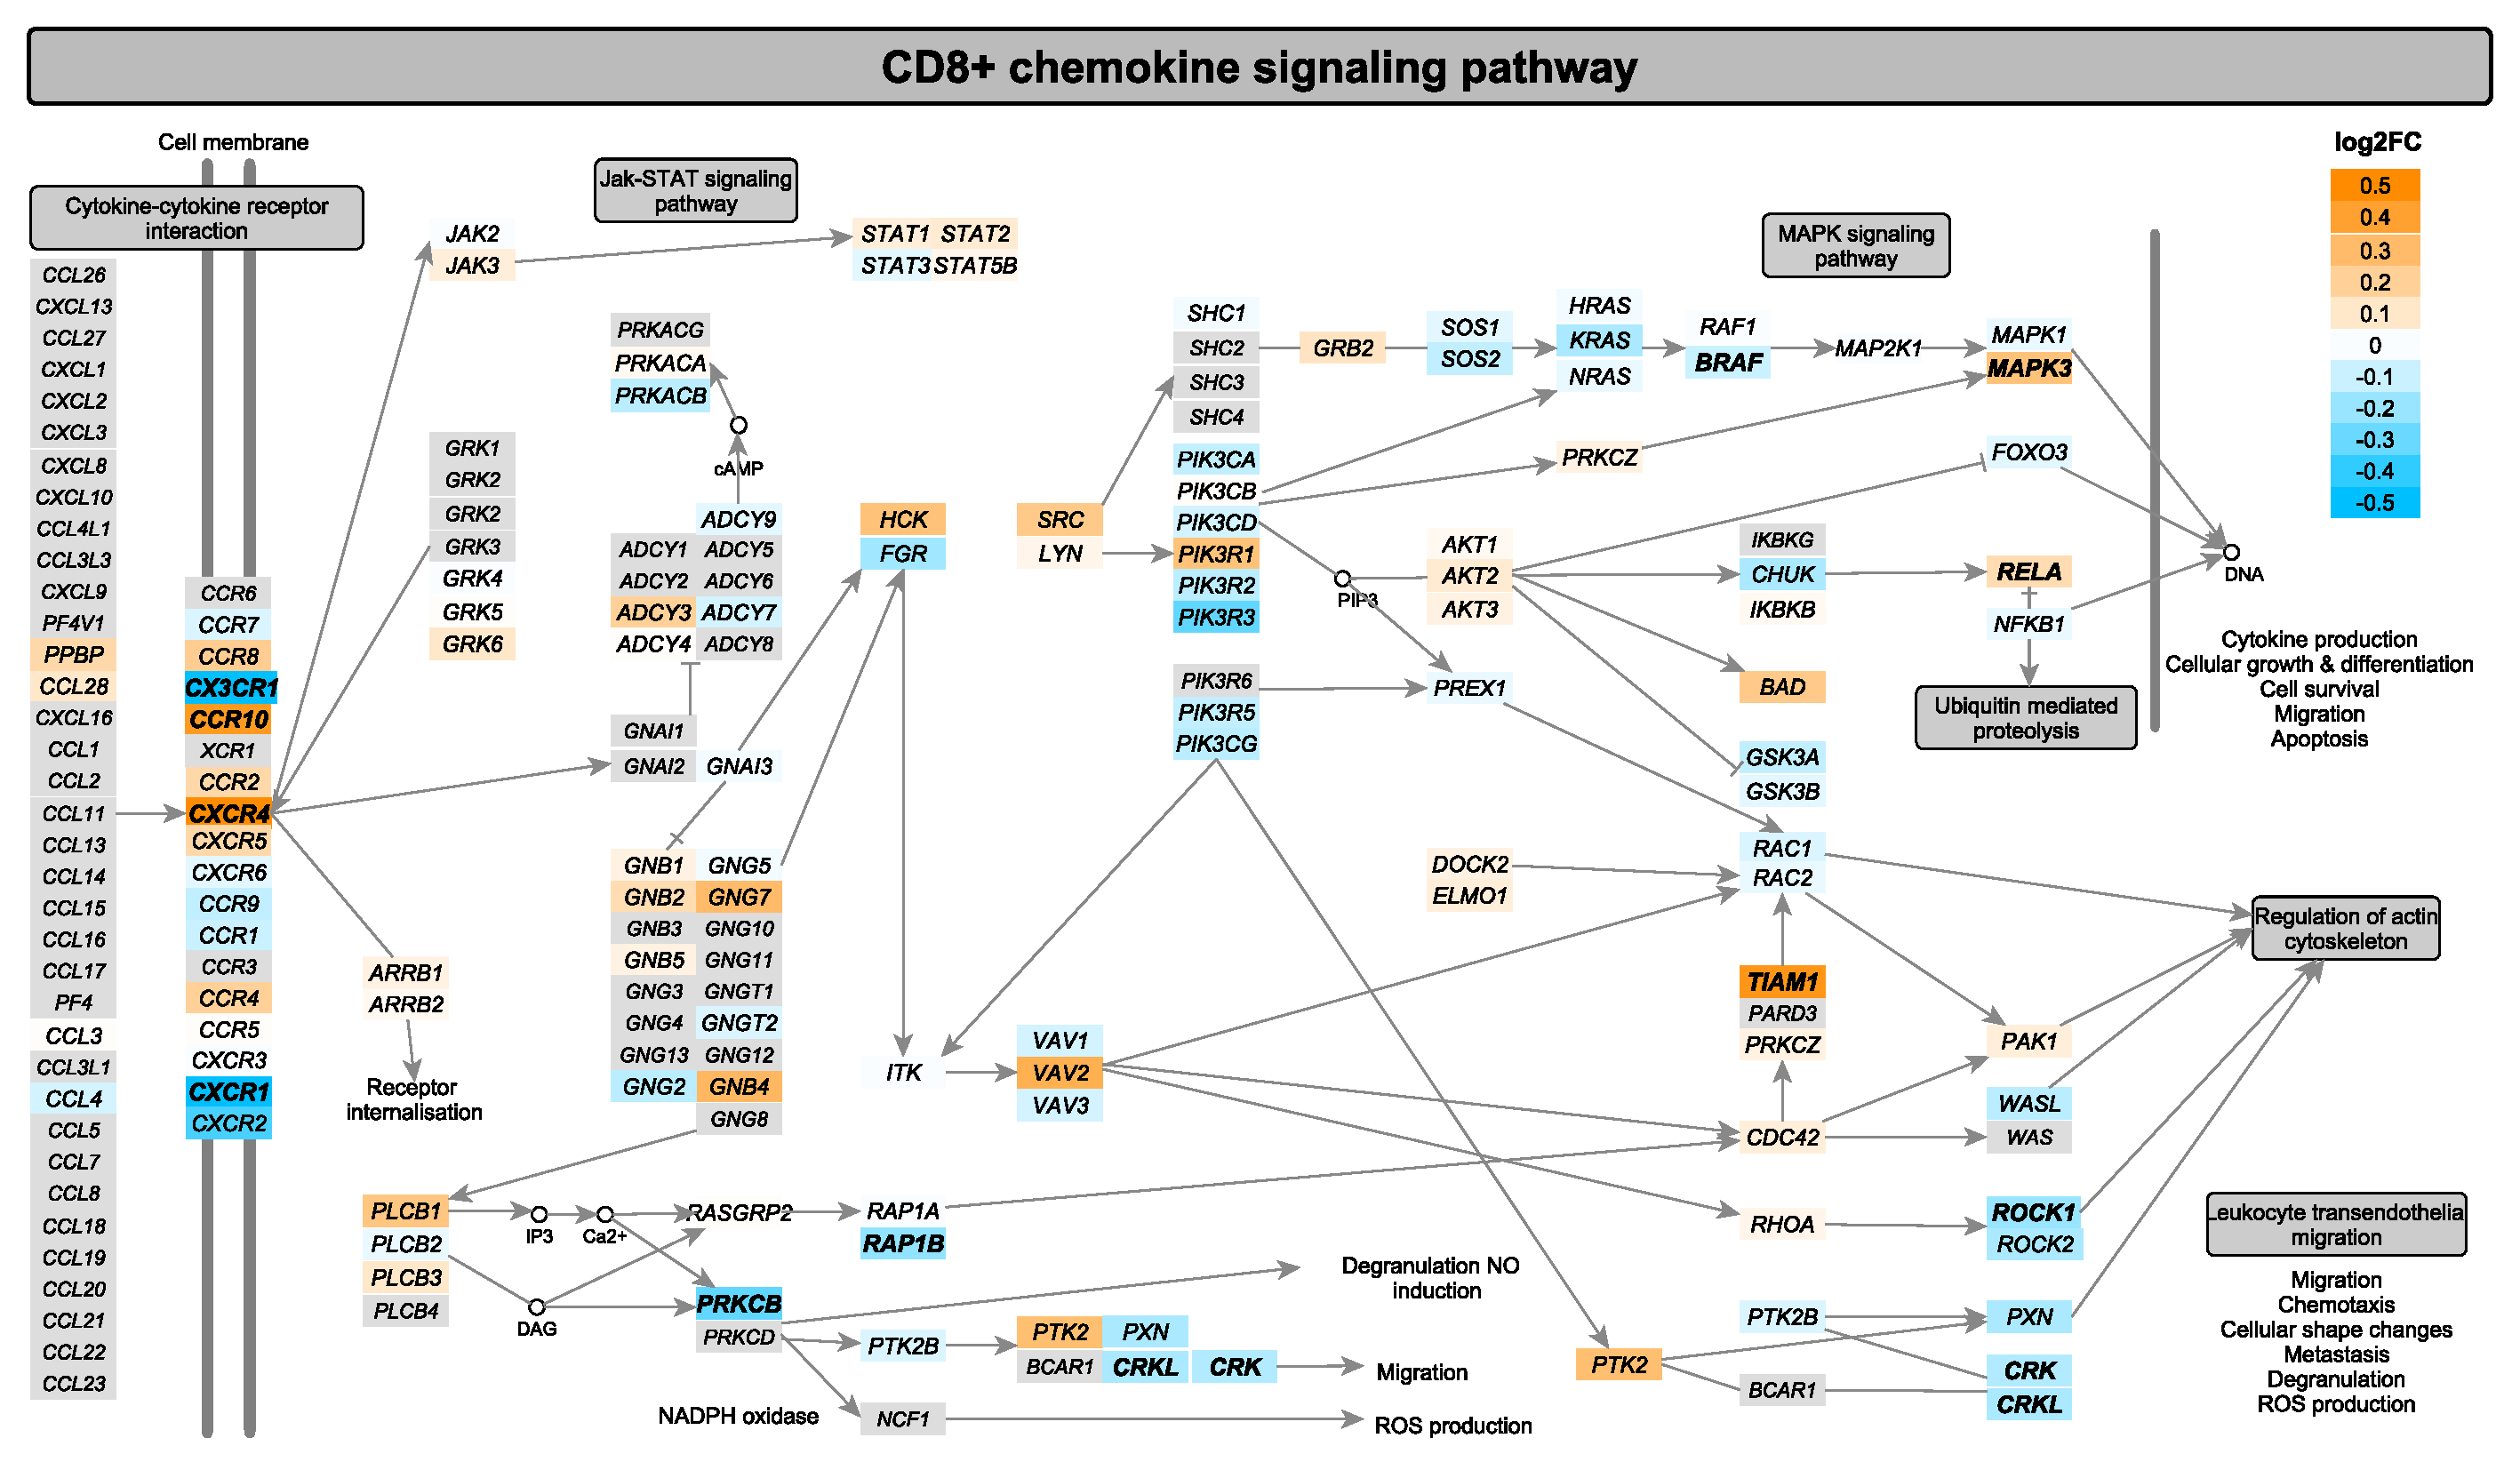
\includegraphics[width=\textwidth]{./Results2/pdfs/PS_CTL_CD8_all_chemokine_pathway}
\caption{\textbf{}}
\end{subfigure}
\caption[Mapping of the DEGs identified in CD8$^+$ cells between psoriasis patients and healthy controls onto the TNF-$\alpha$ and the chemokine signalling pathways.]{\textbf{Mapping of the DEGs identified in CD8$^+$ cells between psoriasis patients and healthy controls onto the TNF-$\alpha$ and the chemokine signalling pathways.} The (A) TNF-$\alpha$ and (B) chemokine pathways were sourced from KEGG, manually curated in a way that all member genes are maximised visually and then automatically color-coded by the log$_2$fold change expression between psoriasis patients and healthy controls CD8$^+$ cells isolated from PB. Significant DEGs (FDR$<$0.05) are highlighted in bold. In (A), members of the TNF-$\alpha$ pathway shared with the NF-$\kappa$B are highlighted with a green box. Additional members of the NF-$\kappa$B pathway differentially regulated in CD8$^+$ cells have also been indicated in brackets. Enrichment for (A) and (B) was identified by using only the CD8$^+$ DEGs (FDR$<$0.05).}
\label{figure:RNAseq_PS_CTL_CD8_TNF_and_chemokine_pathway_modified}
\end{figure}



%Genes such as the activating transcription factor 2 (\textit{ATF2}) and 4 (\textit{ATF4}) members of the TNF signalling cascade and the protein kinase C beta\textit{PRKCB} from the NF-$\kappa$B and chemokine signalling pathways appeared down-regulated in psoriasis vs healthy controls. In contrast, JunB proto-oncogene (\textit{JUNB}) coding for one of the subunits of the TF AP-1 and three of the NF-$\kappa$B subunits including \textit{RELA}, \textit{RELB} and \textit{NFKB2} showed up-regulation in patients vs controls. Particularly, AP-1, undergoes activation following growth factors, cytokines, chemokines, hormones and multiple environmental stresses and acts as a negative regulator of cell proliferation and IL-6 production \parencite{Schonthaler2011}.

%Genes with prominent pro-inflammatory role in the NF-$\kappa$B or TNF signalling pathways also appeared to be down-regulated, such as the activating transcription factor 2 (\textit{ATF2}) and 4 (\textit{ATF4}) members of the TNF signalling cascade and the protein kinase C beta\textit{PRKCB} from the NF-$\kappa$B and chemokine signalling pathways. Up-regulation of pro-inflammatory genes JunB proto-oncogene (\textit{JUNB}) coding for one of the subunits of the TF AP-1 and three of the NF-$\kappa$B subunits including \textit{RELA}, \textit{RELB} and \textit{NFKB2}. 




%https://www.ncbi.nlm.nih.gov/pmc/articles/PMC3884931/
% role of SLA in monocytes http://www.jimmunol.org/content/186/4/1923.long

%Some studies have demonstrated an increased of CCR10$^+$ infiltrated T lymphocytes in psoriasis \parencite{Homey2002}. In circulation, expression of CCR10 is restricted to the a subset of circulating mCD4$^+$ and mCD8$^+$ T cells expressing the cutaneous lymphocyte-associated antigen (CLA), which are preferentially recruited to cutaneous sites of inflammation where KCs express CCL27 \parencite{Hudak2002}. A study in psoriasis circulating cells revealed a correlation between the frequency of CTLA$^+$ CD8$^+$ cells and disease severity measured by PASI score \parencite{Sigmundsd\'{o}ttir2001}. Other up-regulated chemokine receptors in CD8$^+$ circulating psoriatic cells included \textit{CXCR4} gene (receptor for CXCL12) for which ?conflicting findings have been reported about its role in skin inflammation and psoriasis \parencite{Zgraggen2014,Takekoshi2013}.

%TNF:
% ATF4 https://www.tandfonline.com/doi/full/10.1080/15548627.2016.1156823
%JUNB up in psoriasis https://www.jidonline.org/article/S0022-202X(15)32827-X/fulltext;https://www.ncbi.nlm.nih.gov/pubmed/15377346
%PKCB https://www.ncbi.nlm.nih.gov/pmc/articles/PMC5594653/


\subsection{RNA-seq in epidermis from psoriasis patients}

\subsubsection{Data processing and quality control}
All three paired uninvolved-lesional samples (Table \ref{tab:Psoriasis_cohort_metadata}) had a mapping rate greater than 80\% (Figure \ref{figure:RNAseq_PS_uninvolved_lesional_psoriasis_skin_mapping}A) and showed between 29.5 and 33.2 million reads mapping to Ensembl genes after filtering (Figure \ref{figure:RNAseq_PS_uninvolved_lesional_psoriasis_skin_mapping}B). The mapping rate and final number of reads mapping to genes was greater in the lesional samples compared to the controls (Figure \ref{figure:RNAseq_PS_uninvolved_lesional_psoriasis_skin_mapping}). PCA using normalised number of reads mapping to genes showed substantial variation between the lesional and uninvolved samples (Figure \ref{figure:RNAseq_PS_lesional_uninvolved_PCA}), PC1 37\% of the variance) together with biological variability across individuals (PC2, 30\% of the variance), for which the subsequent paired design in the differential gene expression analysis accounted.  


\begin{figure}[htbp]
\centering
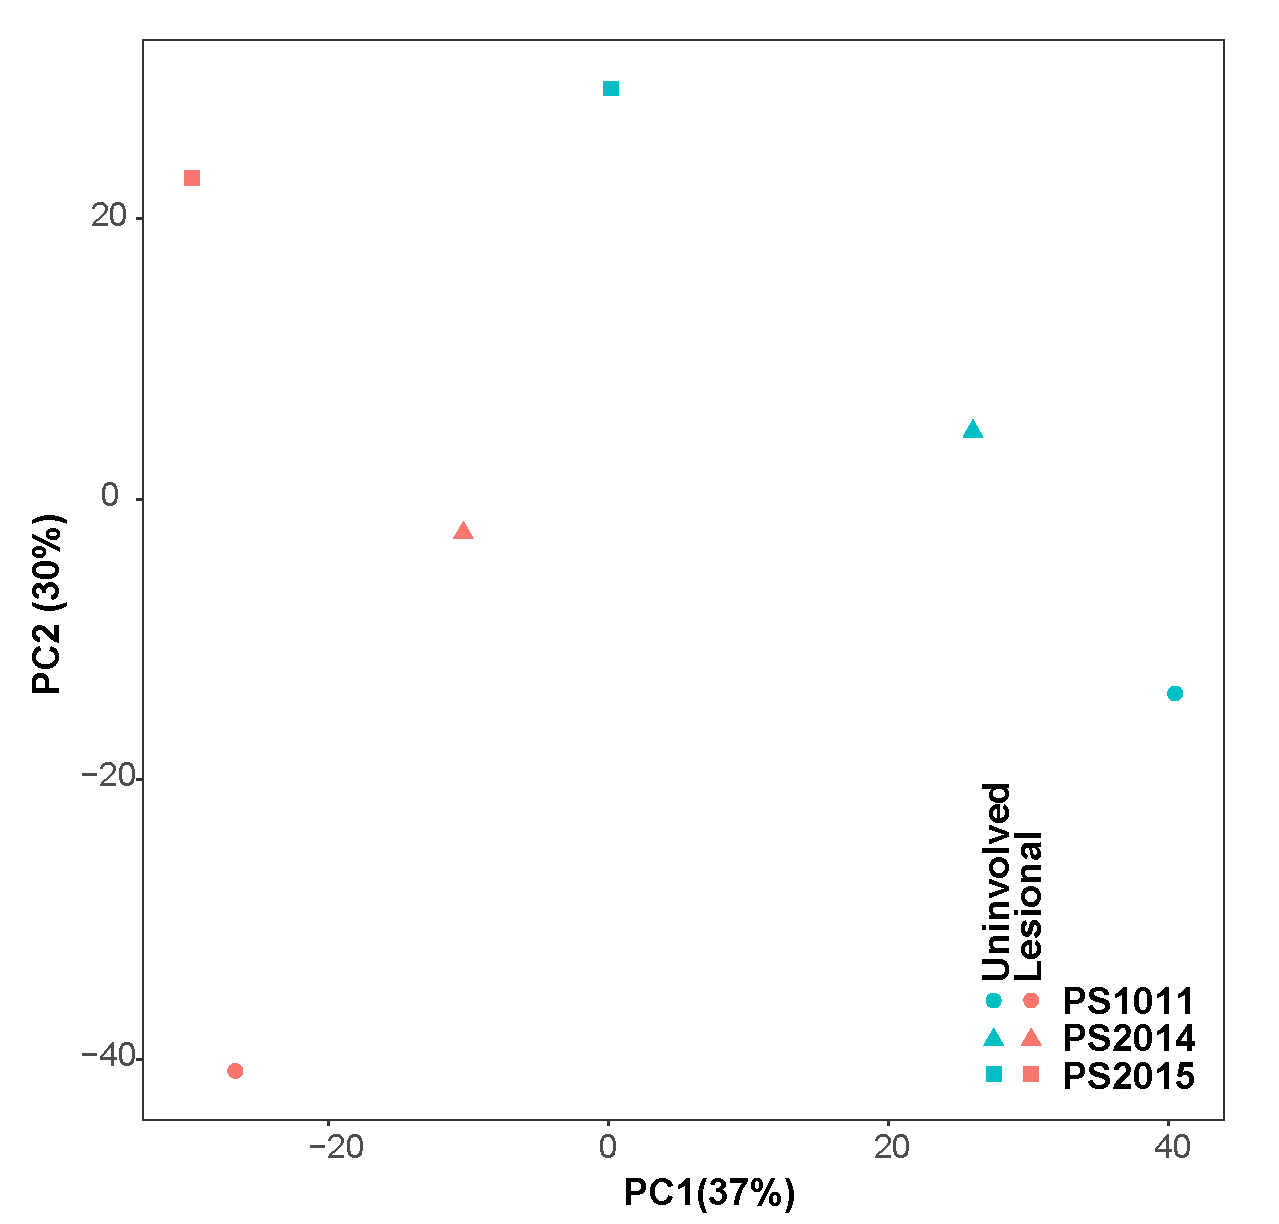
\includegraphics[width=0.5\textwidth]{./Results2/pdfs/PS_lesional_uninvolved_varied_PCA1and2_plot}
\caption[PCA for RNA-seq in the uninvolved and lesional epidermis from psoriasis patients.]{\textbf{PCA for RNA-seq in the uninvolved and lesional epidermis from psoriasis patients.} First and second component of the PCA performed on the normalised number of reads mapping to the Ensmbl list of mRNAs and lncRNAs detected in lesional and uninvolved epidermis isolated from psoriasis patient skin biopsies. Colour corresponds to condition (lesional or uninvolved) and shape refers to the patient ID.}
\label{figure:RNAseq_PS_lesional_uninvolved_PCA}
\end{figure}




\subsubsection{Summary of differential gene expression between lesional and uninvolved epidermis}

Differential gene expression analysis revealed a total of 1,227 (FDR$<$0.05) or 702 (FDR$<$0.01) genes differentially expressed between uninvolved and lesional epidermis skin biopsies, including mRNAs and lncRNAs (Table \ref{tab:RNAseq_PS_lesional_uninvolved_DGE_results}). Amongst the 1,227 DEGs, a similar proportion of up- and down-regulated genes (559 and 629, respectively) were identified between lesional and uninvolved epidermis (Figure \ref{figure:Skin_DGE_volcano_plot}) and 46 were annotated as lncRNAs (Table \ref{tab:RNAseq_PS_lesional_uninvolved_DGE_results}). The magnitude of changes in gene expression between lesional and uninvolved skin were notably larger when compared to the changes in expression in peripheral blood, with 874 out of 1,227 genes showing fold change$>$1.5.  


\begin{table}[htbp]
%\setlength{\tabcolsep}{20pt} only to stretch the columns if you want
%\renewcommand{\arraystretch}{1.5}
\centering
\begin{tabular}{@{} c c c c}
\toprule
\textbf{FDR threshold}   & \textbf{mRNA}   & \textbf{lncRNA}  & \textbf{Overlap with}\\
                         &                 &                  & \textbf{GWAS genes}\\
\midrule
\midrule
0.05                     & 1181            & 46               &  up(\textit{IFIH1}, \textit{NOS2}, \textit{STAT3},\\ 
                         &                 &                  &  \textit{LCE3D}), down(\textit{TNFAIP3}) \\
0.01                     &  677            & 25               &  \textit{NOS2}, \textit{STAT3},\textit{TNFAIP3},\textit{LCE3D} \\
\bottomrule 
\end{tabular}
\medskip %gap
\caption[Summary of the differential gene expression analysis between uninvolved and lesional psoriatic epidermal biopsies.]{\textbf{Summary of the differential gene expression analysis between uninvolved and lesional psoriatic epidermal biopsies.} Number of differentially expressed mRNAs and lncRNAs are reported for two thresholds of significance (FDR$<$0.05 and FDR$<$0.01). The DEGs overlapping putative psoriasis GWAS genes and the directionality in the change of expression are listed.}
\label{tab:RNAseq_PS_lesional_uninvolved_DGE_results}
\end{table}
\bigskip %bigger spac



Amongst DEGs between the uninvolved and lesional skin, five genes (FDR$<$0.05) overlapped with putative GWAS genes (Table \ref{tab:RNAseq_PS_lesional_uninvolved_DGE_results}). \textit{IFIH1} (fold change=1.47), \textit{NOS2} (fold change=1.74), \textit{LCE3D} (fold change=1.94) and \textit{STAT3} (fold change=1.54) were up-regulated in lesional epidermis, whereas \textit{TNFAIP3} was down-regulated (fold change=0.47). All these genes but \textit{IFIH1} showed significant differential expression at the more stringet FDR$<$0.01 threshold.

%\textit{IFIH1}, \textit{NOS2}, \textit{LCE3D} and \textit{STAT3} were also found to be up-regulated in lesional compared to uninvolved skin biopsies from psoriasis patients in \parencite{Tsoi2015}. In contrast, \textit{TFNAIP3} was found to be up-regulated in \parencite{Jabbari2012}, opposite to our finding.
\begin{figure}[htbp]
\centering
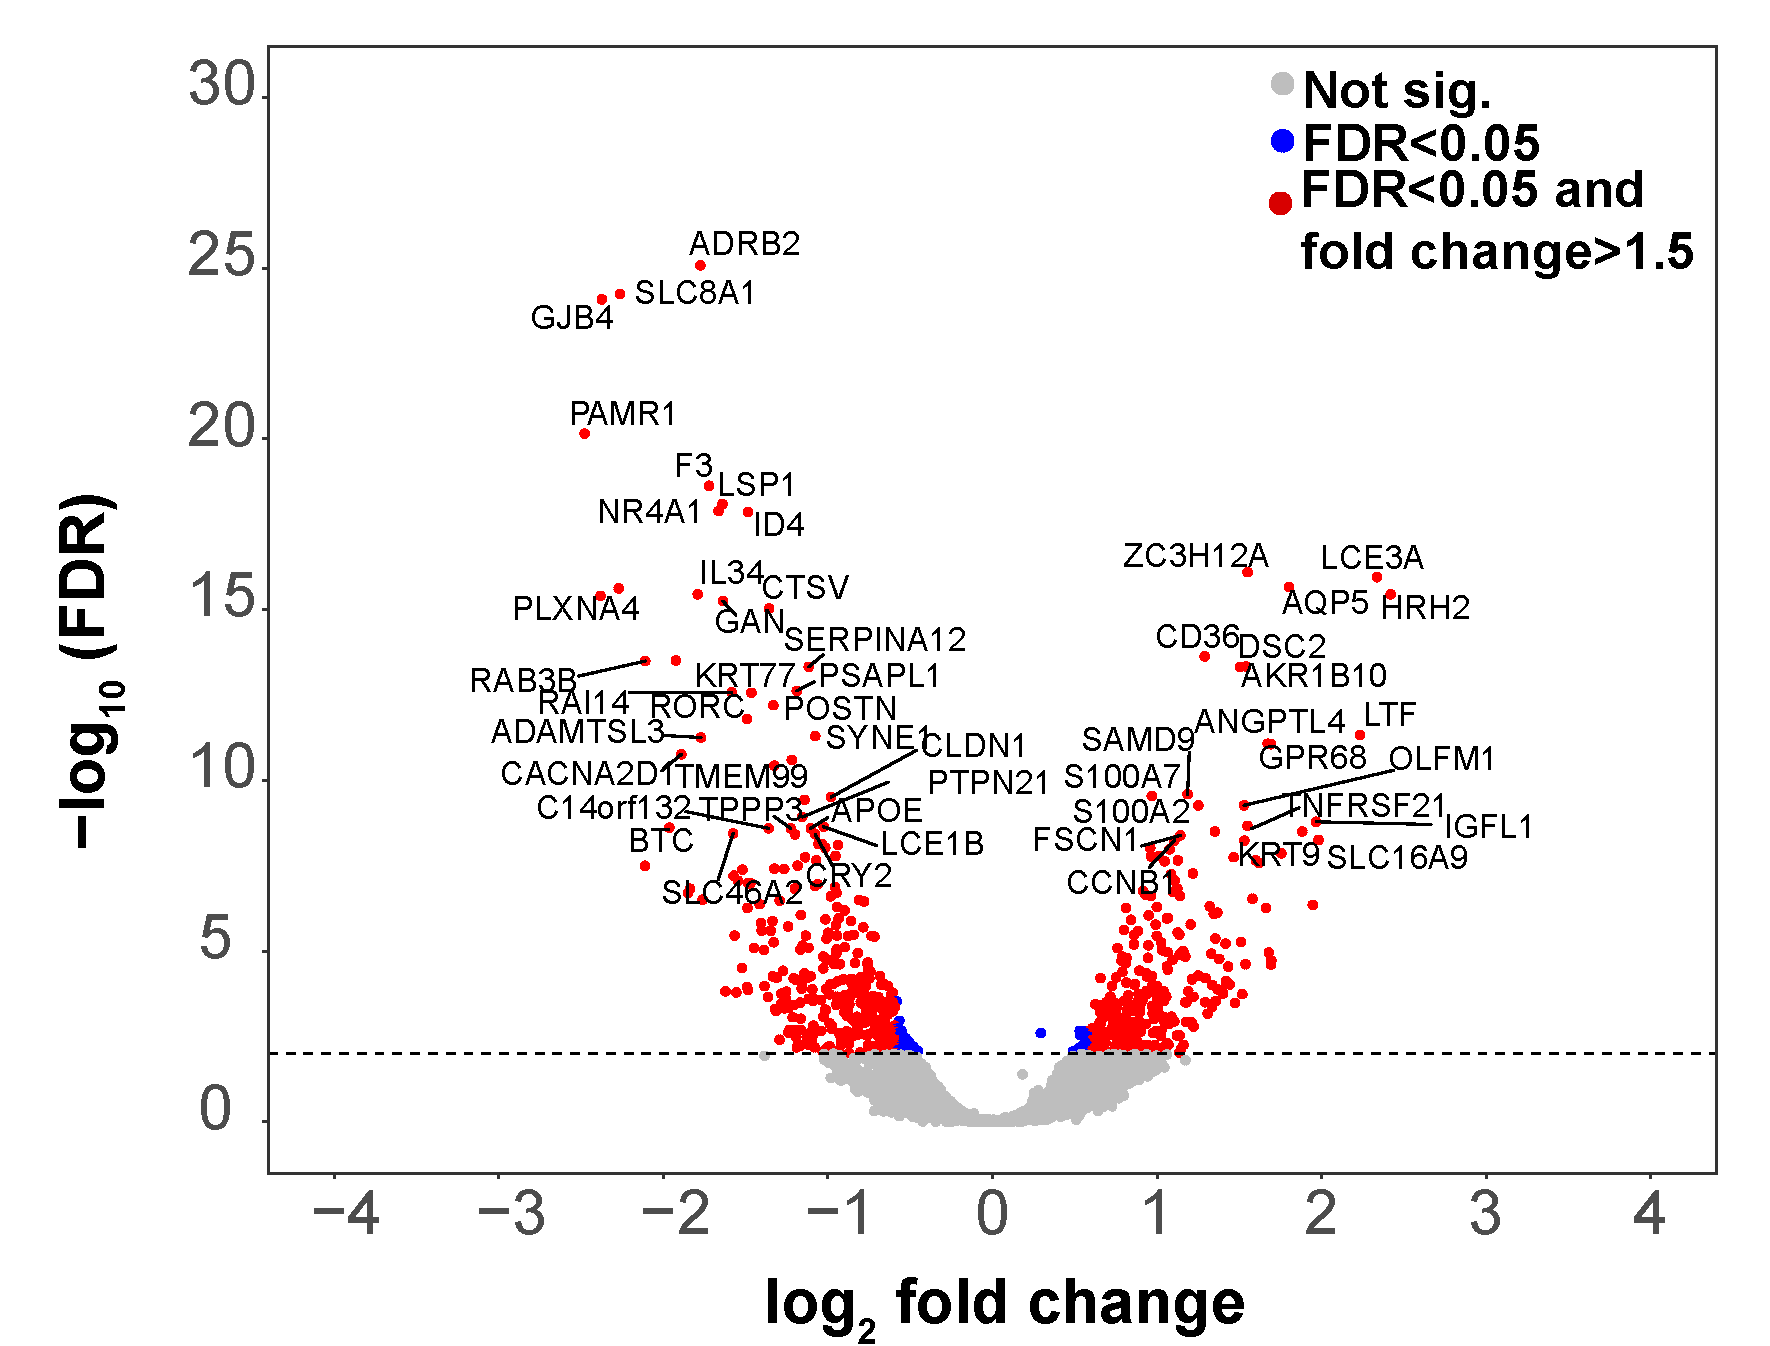
\includegraphics[width=0.6\textwidth]{./Results2/pdfs/RNA_PS_lesional_uninvolved_volcano_plot}
\caption[Magnitude and significance of the gene expression changes between matched lesional and uninvolved epidermal biopsies from three psoriasis patients.]{\textbf{Magnitude and significance of the gene expression changes between matched lesional and uninvolved epidermal biopsies from three psoriasis patients.} The volcano plot represents for each gene the significance (-log$_{10}FDR$) of the log$_2$fold change in expression for that gene in lesional skin group vs uninvolved skin. Significant DEGs (FDR$<$0.05) in blue for fold change$<$1.5 and red for fold change$>$1.5. The volcano plot includes mRNAs and lncRNAs species.}
\label{figure:Skin_DGE_volcano_plot}
\end{figure}





\subsubsection{Comparison with other skin transcriptomic studies}

As detailed in Chapter \ref{ch:Mat}, in this thesis the epidermal layer was isolated from the rest of the biopsy in contrast to most published transcriptomic studies using full-thickness biopsies to compare lesional and uninvolved skin from psoriasis patients. This allowed to obtain purer sample composition with the majority of cells being epidermal keratinocytes and a smaller proportion infiltrated immune cells. During the course of this project a study was published by Tervaniemi and colleagues characterising the transcriptional profiles epidermis from lesional and uninvolved psoriatic skin \parencite{Tervaniemi2016}. %As previously detailed, Tevaniemi \textit{et al.} had a bigger sample size (six psoriasis patients) compared to this study (three psoriasis patients) and also included nine control epidermis biopsies. 
In order to explore the similarities across the two studies, a comparison of DEGs identified between lesional and uninvolved matched samples was conducted. 


The Tervaniemi study identified 2,589 DEGs (filtering criteria fold change$<$0.75 or fold change$>$1.5 and FDR$<$0.05), a larger number of DEGs compared to the number found here, and reported a greater number of up-regulated than down-regulated hits (Figure \ref{figure:Skin_venn_diagrams_comparison_other_studies} bottom panel). A total of 359 out of the 1,227 DEGs (29.25\%) identified here were shared with the Tervaniemi results, of which 239 and 75 were up- and down-regulated, respectively (Figure \ref{figure:Skin_venn_diagrams_comparison_other_studies} bottom panel). Some examples of this overlap included up-regulation of \textit{STAT1}, genes from the \textit{S100} family (e.g \textit{S100A9} and \textit{S100A12}) and genes nearby psoriasis GWAS loci such as \textit{STAT3} and \textit{IFIH1}. Notably, 45 genes were differentially expressed in both studies but showed opposite direction. For example \textit{SERPINB2} was down-regulated in this study and up-regulated in the Tervaniemi results. 


%Tervaniemi reported a total of 2,589 DEGs passing their filtering criteria (fold change$<$0.75 or fold change$>$1.5 and FDR$<$0.05) and showing overall a larger number of differentially expressed genes between the two types of biopsies compared this study. The number of genes up-regulated in lesional epidermis compared to uninvolved (2,330) was larger than the number of down-regulated targets (261), contrasting to the in-house results where similar numbers of up- and down-regulated genes were found (Table \ref{RNAseq_PS_lesional_uninvolved_DGE_results} and Figure \ref{figure:Skin_venn_diagrams_comparison_other_studies} bottom panel). Regarding overlap, a total of 359 out of the 1,227 DEGs (29.25\%) identified by the in-house study were shared with the Tervaniemi results, of which 239 and 75 were up- and down-regulated, respectively. Amongst the up-regulated genes in both studies TFs such as \textit{STAT1}, genes from the \textit{S100} family (e.g \textit{S100A9} and \textit{S100A12}) and genes nearby psoriasis GWAS loci such as \textit{STAT3} and \textit{IFIH1}. The direction of change in 45 out of the 359 shared genes appeared to be opposite across the two datasets. For example, \textit{SERPINB2} gene, a serine protease inhibitor of the serpin superfamily, presented down-regulation in the in-house data and up-regulation in the Tervaniemi results. Interestingly, a study demonstrated a defective stratum corneum in \textit{SERPINB2} deficient mice as well as greater susceptibility to developing inflammatory lesions upon chemically induced atopic dermatitis compared to wild type controls \parencite{Schroder2016}. 


%The direction of change in 45 out of the 359 shared genes appeared to be opposite across the two datasets. For example, \textit{SERPINB2} gene, a serine protease inhibitor of the serpin superfamily,presented down-regulation in the in-house data and cultured lesional KCs from Swindell \textit{et al.}, 2017 in contrast to the up-regulation in the Tervaniemi results. Interestingly, a study demonstrated a defective stratum corneum in \textit{SERPINB2} deficient mice as well as greater susceptibility to developing inflammatory lesions upon chemically induced atopic dermatitis compared to wild type controls \parencite{Schroder2016}.   


Additionally, these results were also contrasted with one of the most recent comprehensive RNA-seq studies comparing lesional and uninvolved full-thickness skin biopsies from psoriasis patients \parencite{Tsoi2015}. Out of the 3,725 DEGs reported by the Tsoi analysis, 507 genes were shared between the two studies (41\% of the in-house DEGs), of which 24 corresponded to dysregulated lncRNAs. Amongst the 507 commonly dysregulated genes, 272 were up-regulated, 228 down-regulated and only 7 showed opposite direction of change (Figure \ref{figure:Skin_venn_diagrams_comparison_other_studies} top panel). %Some of the genes found dysregulated in the same direction between the in-house and Tervaniemi's stuy were also consistently dysregulated in Tsoi analysis, including \textit{STAT1}, \textit{S100} and the GWAS genes \textit{STAT3} and \textit{IFIH1}. Moreover, the GWAS gene \textit{NOS2} was also a shared up-regulated hit with Tsoi's data, which was noy fooud to be dysregulated in Tervaniemi's analysis. The genes showing dysregulation in the opposite direction included \textit{ALOX15B},  \textit{ARG2}, \textit{LCE6A},\textit{MGST1}, \textit{PNLIPRP3}, \textit{TLDC1} and \textit{UBL3}. For example, \textit{LCE6A}, a member of the\textit{LCE} family involved in the synthesis of the later cornified envelope layer, was down-regulated in lesional skin in our study, in contrast to the up-regulation found in the Tsoi analysis. Notably, down-regulation of genes from the LCE family, including \textit{LCE1B}, \textit{LCE1F} and \textit{LCE2A}, showed opposite direction of change in both, Tsoi and Tervaniemi's analyses. An study performing qPCR quantification of \textit{LCE} genes from groups 1, 2, 5 and 6 demonstrated increased expression in psoriasis lesional skin, in line with the in-house results \parencite{Bergboer2011}. In contrast to the other genes from the \textit{LCE} family, all three datasets presented up-regulation of the GWAS risk associated gene \textit{LCE3B}. 

Simultanous overlap across the three studies identified only 212 DEGs. Despite having a larger sample size, the Tsoi study did not capture the majority of the DEGs from this dataset or the Tervaniemi one (Figure \ref{figure:Skin_venn_diagrams_comparison_other_studies} middle panel). %This may suggest, amongst other things, some of the DEGs being specific to the type of biopsy used on each approach. 
%Notably, qPCR quantification of \textit{LCE} genes from groups 1, 2, 5 and 6 demonstrated increased expression in psoriasis lesional skin \parencite{Bergboer2011}. 


%Overall, the comparison of our results with these two studies suggested greater similarities with the full skin thickness biopsies from Tsoi \textit{et al.}, 2015 in terms of DEGs overlapping, due to different technical reasons as further detailed in the Discussion. 

\begin{figure}[ht]
\centering
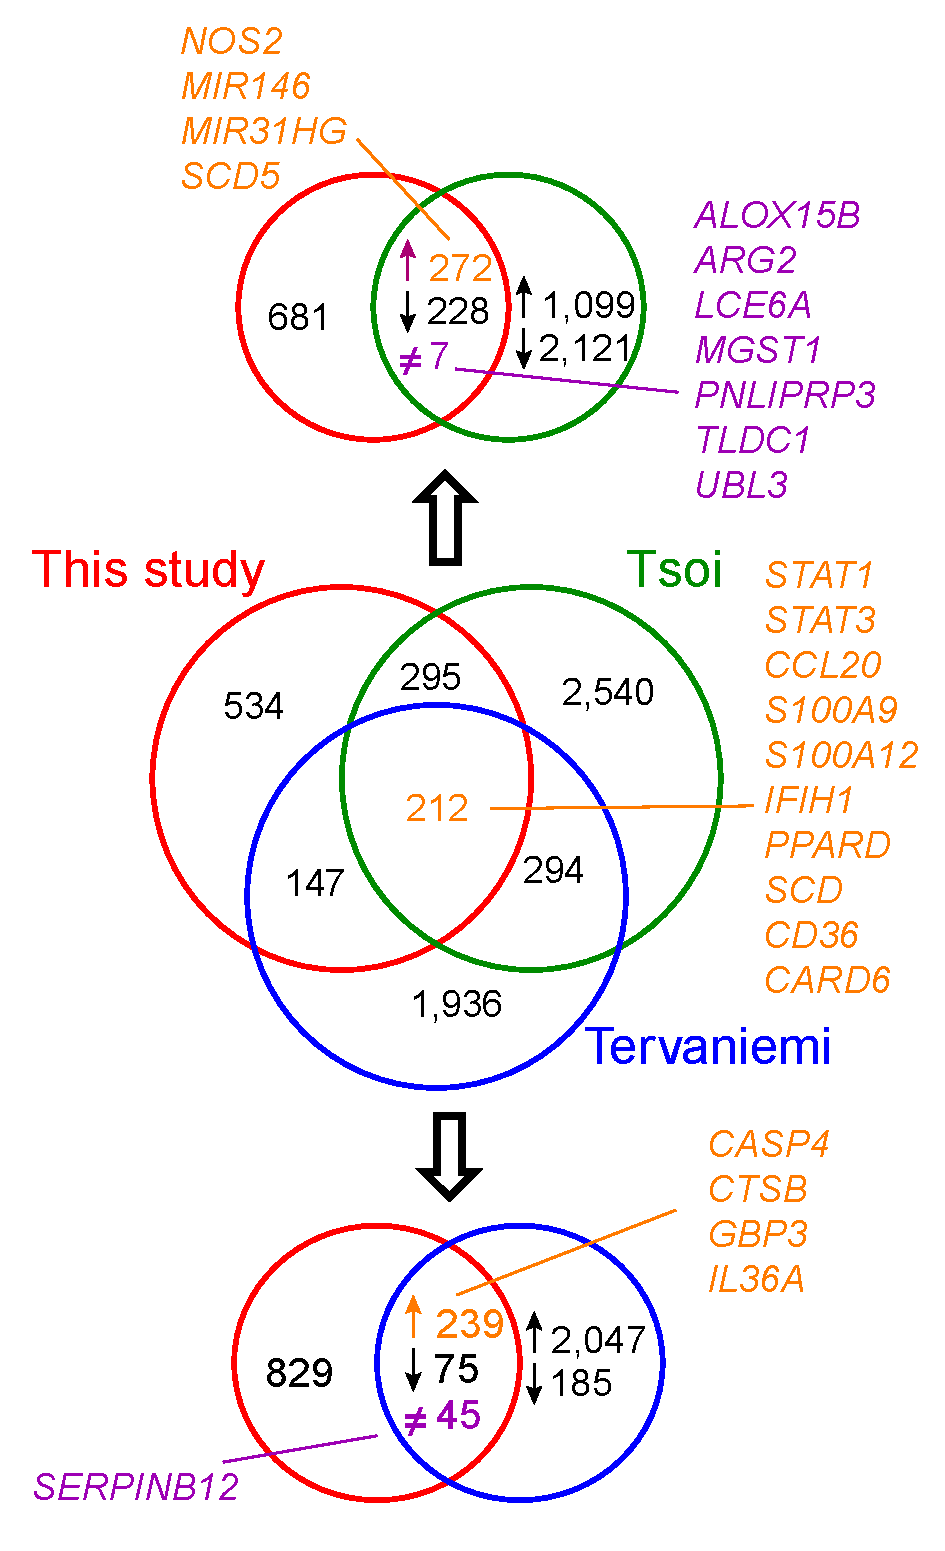
\includegraphics[width=0.5\textwidth]{./Results2/pdfs/skin_transcriptomics_venn_diagrams_with_genes}
\caption[Overlap of the significantly differentially expressed genes between lesional and uninvolved epidermal sheets, split epidermis and full-thickness skin biopsies.]{\textbf{Overlap of the significantly differentially expressed genes between lesional and uninvolved epidermal sheets, split epidermis and full-thickness skin biopsies.} The central venn diagram illustrated the DEGs overlapping between this study, Tervaniemi \textit{et al.} 2016 psoriasis split epidermis biopsies and Tsoi \textit{et al.} 2015a full-thickness psoriasis skin biopsies. Overlap is considered regardless the direction of the change. Two additional venn diagrams provide more detail about the total overlap and directionality in the change of gene expression between the in-house data and the Tsoi \textit{et al.} 2015a (top) or Tervaniemi \textit{et al.} (bottom). Some of overlapping genes are listed.}
\label{figure:Skin_venn_diagrams_comparison_other_studies}
\end{figure}





\subsubsection{Dysregulated lncRNAs in the psoriatic lesional skin}

In addition to protein coding genes, 46 lncRNAs were significantly (FDR$<$0.05) differentially expressed between uninvolved and lesional skin and 37 of them had an interacting partner experimetally validated according to NPInter database \parencite{Hao2016}. An interesting  example was \textit{H19}, which was significantly down-regulated (fold-change=0.43) in lesional epidermis and has been described to directly bind miR-130b-3p, which down-regulates desmoglein 1 (\textit{DSG1}), a gene promoting keratinocyte differentiation \parencite{Li2017}. Nevertheless, \textit{DSG1} itself did not show differential expression between lesional and uninvolved skin. %This finding was consistent with Tsoi \textit{et al.}, 2015 and also with results from Li \textit{et al.}, 2014 and ?\textit{et al.}, 2016 where they compared lesional versus normal skin. 

Interestingly, four miRNAs (\textit{MIR146A}, \textit{MIR22HG}, \textit{MIR31HG} and \textit{MIR205HG}) were also captured with the standard library preparation for mRNAs and lncRNAs. The relevance of miR-146a has been already noted in the differential analysis from circulating immune cells (Section 3.3.4). In lesional skin \textit{MIR146A} was up-regulated (fold change=2.0) when compared to uninvolved skin, consistent with other studies \parencite{Lerman2011, Tsoi2015}. %and was also shown to have increased expression when comparing lesional skin versus healthy biopsies \parencite{Li2014}. One of the predicted miR-146a targets by Target Rank software in a study conducted by Jazdzewski and colleagues revealed \textit{NFAT5}, also down-regulated in lesional skin compared to uninvolved in the in-house data, as the 11$^{th}$ most confidently predicted target \parencite{Jazdzewski2009}. Interestingly, a negative correlation (R=-0.981, p-value=5.3x10$^{-4}$) between the normalised counts of the two genes was found in the three lesional-uninvolved paired samples (Figure \ref{figure:RNAseq_lesional_uninvolved_miR_correlations} a).
%check if target genes dysregulated https://www.pnas.org/content/106/5/1502
%Moreover, a polymorphism in miR-146a has been associated with psoriasis in a small cohort study and a \textit{MIR146A} knock-out mice with chemical induced psoriasis led to earlier disease onset and amplified epidermal activation \parencite{Srivastava2017}. 


%\begin{figure}[htbp]
%\centering
%\begin{subfigure}{0.45\textwidth}
%\centering
%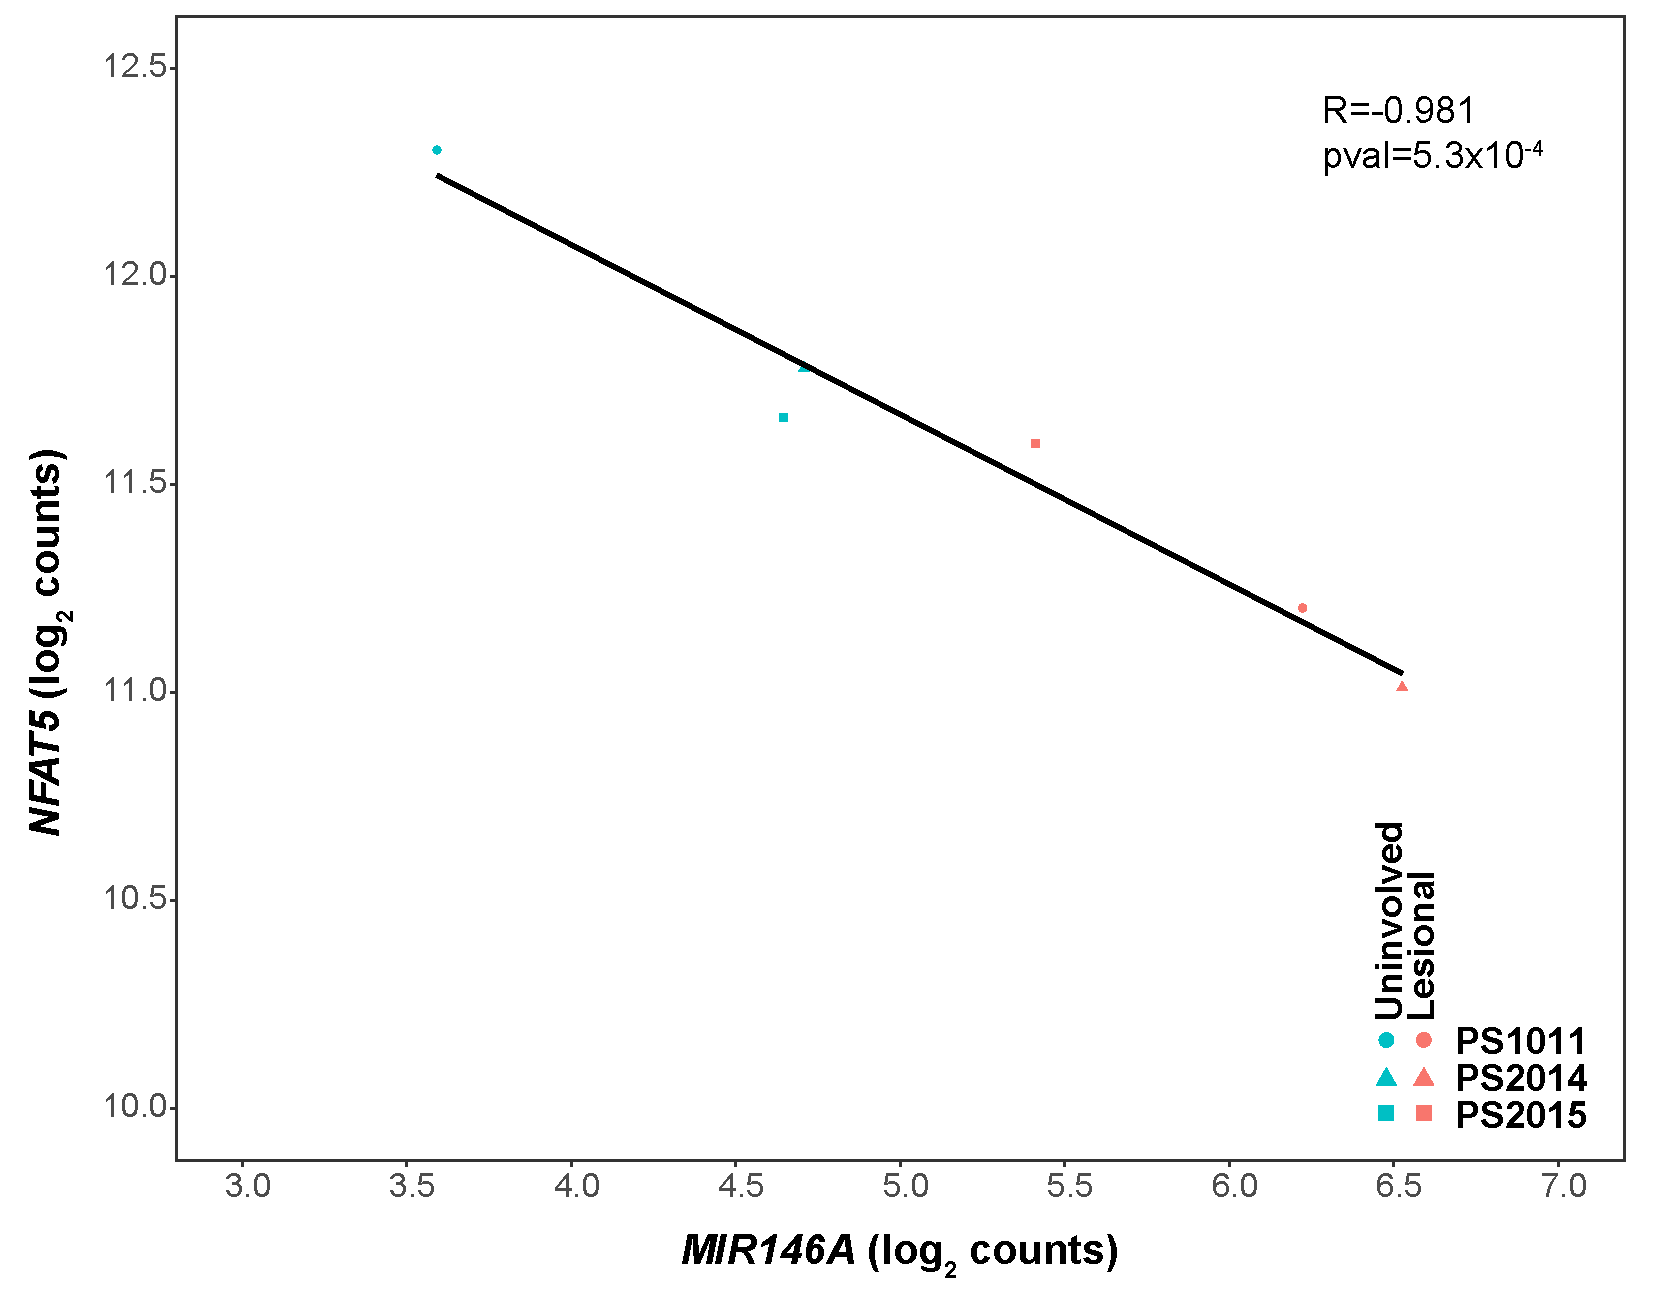
\includegraphics[width=\textwidth]{./Results2/pdfs/Skin_RNAseq_correlation_MIR146A_NFAT5_plot}
%\caption{\textbf{}}
%% The percentage sign indicated that the other subfig goes side by side
%\end{subfigure}%
%\begin{subfigure}{0.45 \textwidth}
%\centering
%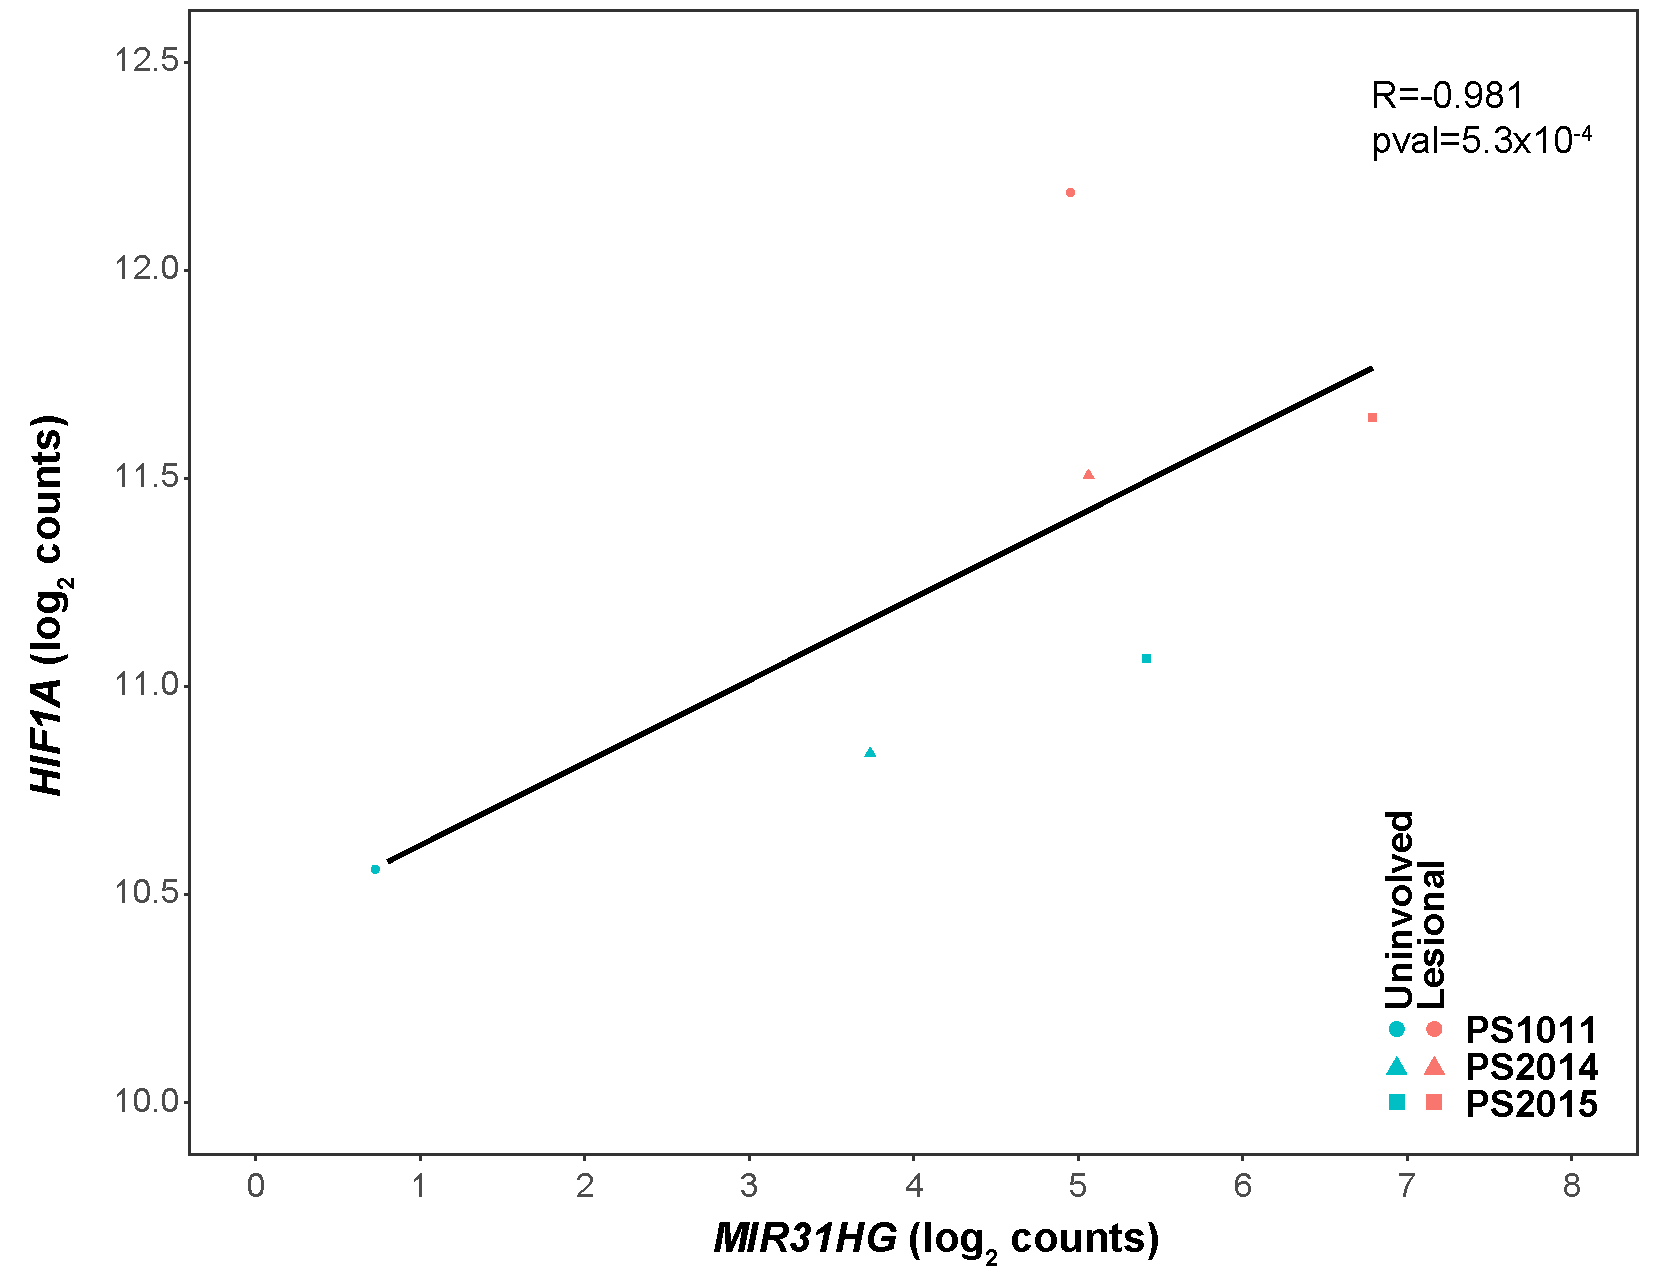
\includegraphics[width=\textwidth]{./Results2/pdfs/Skin_RNAseq_correlation_MIR31HG_HIF1A_plot}
%\caption{\textbf{}}
%\end{subfigure}
%\caption[Correlation in gene expression between two dyregulated miRs in lesional skin and their putative target genes.]{\textbf{Correlation in gene expression between two dyregulated miRs in lesional skin and their putative target genes.} Plots showing the correlation in log$_2$ normalised read counts for (A) \textit{MIR146A} and its putative target genes \textit{NFAT5} and (B) \textit{MIR31HG} and its putative target genes \textit{HIF-1A}. Pearson correlation values (R) and significance (p-value) are included. Each of the dots represents one samples, where colour represents condition (lesional or uninvolved) and shape corresponds to the patient ID.}
%\label{figure:RNAseq_lesional_uninvolved_miR_correlations}
%\end{figure}



Another relevant finding was the up-regulation of \textit{MIR31HG} (fold change=1.84) in lesional skin previously reported by the Tsoi study \parencite{Tsoi2015}. Additionally, in a study in head and neck carcinoma, \textit{MIR31HG} expression was identified to target \textit{HIF-1A}, inducing up-regulation by an unknown mechanisms \parencite{Wang2018}. In this data, \textit{HIF-1A} was (fold change=1.81) in lesional skin compared to uninvolved, but only a trend for positive correlation was observed between normalised counts of this gene and the putative regulator \textit{MIR31HG} (Figure \ref{figure:RNAseq_lesional_uninvolved_miR_correlations}), likely due to the small sample size.
%Notably, a functional study using the keratinocyte immortal cell line HaCaT demonstrated that silencing miR-31hg induces cell cycle arrest and inhibits cell proliferation consistently with two characteristic functions dysregulated in psoriatic keratinocytes \parencite{Gao2018}.
%also role in osteogenesis https://www.ncbi.nlm.nih.gov/pubmed/27334046
%HIF-1 up-regulation https://molecular-cancer.biomedcentral.com/articles/10.1186/s12943-018-0916-8


%\begin{table}[htbp]
%%\setlength{\tabcolsep}{20pt} only to stretch the columns if you want
%%\renewcommand{\arraystretch}{1.5}
%\centering
%\begin{tabular}{@{} c c c}
%\toprule
%\textbf{Transcript class}   & \textbf{Gupta \textit{et al.},}   & \textbf{Li \textit{et al.}}  \\
                            %& \textbf{2016}                     &      \textit{2014}            \\
%\midrule
%\midrule
%mRNA                        & xxx                               & xxxx                \\
%lncRNAs (functionally       & 2 (\textit{H19} (d),              & 7 (\textit{H19} (d), \textit{NEFL} (d), \textit{SCARNA2} (d),\\
%characterised)              & \textit{LINC00302} (u))           & \textit{SCARNA9} (d), \textit{SCARNA10} (d),\textit{UHRF1} (u),\\
                            %&                                   &  \textit{KCNQ1OT1} (d)) \\
%\bottomrule 
%\end{tabular}
%\medskip %gap
%\caption[Summary results of the DGE analysis between uninvolved and lesional psoriatic epidermal biopsies.]{\textbf{}u=up-regulated; d=down-regulated. Directionality for the differentially expressed lncRNA included in this table was concordant with other studies having reported them previously for all of them but \textit{LINC00302} which appeared down-regulated in this data.}
%\label{tab:RNAseq_PS_lesional_uninvolved_overlap_with_other_studies}
%\end{table}
%\bigskip %bigger spac



\subsubsection{Pathway enrichment analysis}

In order to better understand the functional role of the DEGs (FDR$<$0.05) between lesional and uninvolved epidermis from psoriasis patient skin biopsies, pathways enrichment analysis was conducted. A number of pathways were significantly enriched with FDR$<$0.01 and fold change$>$2 (Tables \ref{tab:RNAseq_PS_lesional_uninvolved_pathway_enrichment} and \ref{tab:RNAseq_PS_lesional_uninvolved_additional_pathways}). 


\begin{table}[htbp]
%\setlength{\tabcolsep}{20pt} only to stretch the columns if you want
\renewcommand{\arraystretch}{0.8}
\centering
\begin{tabular}{@{}c c c}
\toprule
\textbf{Pathway}                      & \textbf{FDR}           & \textbf{Fold change} \\
\midrule
\midrule
IFN-$\alpha$/$\beta$/signalling       &5.4x$10^{-5}$           &3.65                    \\
Peroxisome proliferator-activated     &1.5x$10^{-4}$           &3.42                    \\
receptors (PPAR) & &\\
NOD-like receptor signalling          &3.1x$10^{-4}$           &2.37                  \\
IL-17 signalling                      &1.4x$10^{-3}$           &2.72                    \\
IL2-mediated signalling               &3.1x$10^{-3}$           &2.64                    \\
Hypoxia-inducible factor 1            &5.0x$10^{-3}$           &2.31                     \\
(HIF-1) signalling & &\\
Glycolysis/gluconeogenesis            &1.0x$10^{-6}$           &4.71                     \\
Cell cycle                            &6.7x$10^{-5}$           &2.55                     \\
Apoptosis                             &3.7x$10^{-3}$           &2.11                      \\
Arginine and proline metabolism       &7.5x$10^{-6}$           &5.28                      \\
AGE-RAGE signalling in diabetic complications &8.3x$10^{-3}$  & 2.17 \\
\bottomrule
\end{tabular}
\medskip %gap
\caption[Most relevant pathways enriched for DEGs between lesional and uninvolved epidermis isolated from psoriasis patients skin biopsies.]{\textbf{Most relevant pathways enriched for DEGs between lesional and uninvolved epidermis isolated from psoriasis patients skin biopsies.} Significant pathways for FDR$<$0.01 and fold change$>$2 are listed here and in Table \ref{tab:RNAseq_PS_lesional_uninvolved_additional_pathways}. The analysis was performed using as input significant DEGs (FDR$<$0.05). Enriched pathways had a minimum of ten members overlapping with DEGs.}
\label{tab:RNAseq_PS_lesional_uninvolved_pathway_enrichment}
\end{table}


These included pathways related to alterations in cell cycle and metabolic processes, such as hypoxia-inducible factor 1 (HIF-1) signalling, arginine and proline metabolism, glycolysis/gluconeogenesis and metabolism of carbohydrates. %Dysregulation  of similar functions have previously also been reported in other studies comparing lesional and uninvolved skin and genome-wide pathway analysis\parencite{Coda2012, Aterido2016, Tervaniemi2016}. 
HIF-1 signalling has been found to be up-regulated in psoriatic skin, likely through hypoxia caused by increased cell proliferation rates and epidermal thickening. Here, up-regulation of \textit{HIF1A}, \textit{VEGFA}, \textit{ENO1} and the GWAS gene \textit{NOS2}, amongst others, contributed to the enrichment of this pathway (Figure \ref{figure:PS_lesional_vs_uninvolved_HIF_IL17_pathway}A, in orange and bold). 
%Up-regulated expression of the hypoxia-inducible TFs HIF-1$\alpha$ and HIF-2$\alpha$ has been found in lesional skin and co-related with the increase in \textit{VEGF} transcript levels, a target gene regulated by HIFs that mediates the pathological angiogenesis driving psoriasis \parencite{Rosenberg2007}. 

%\begin{figure}[htbp]
%\centering
%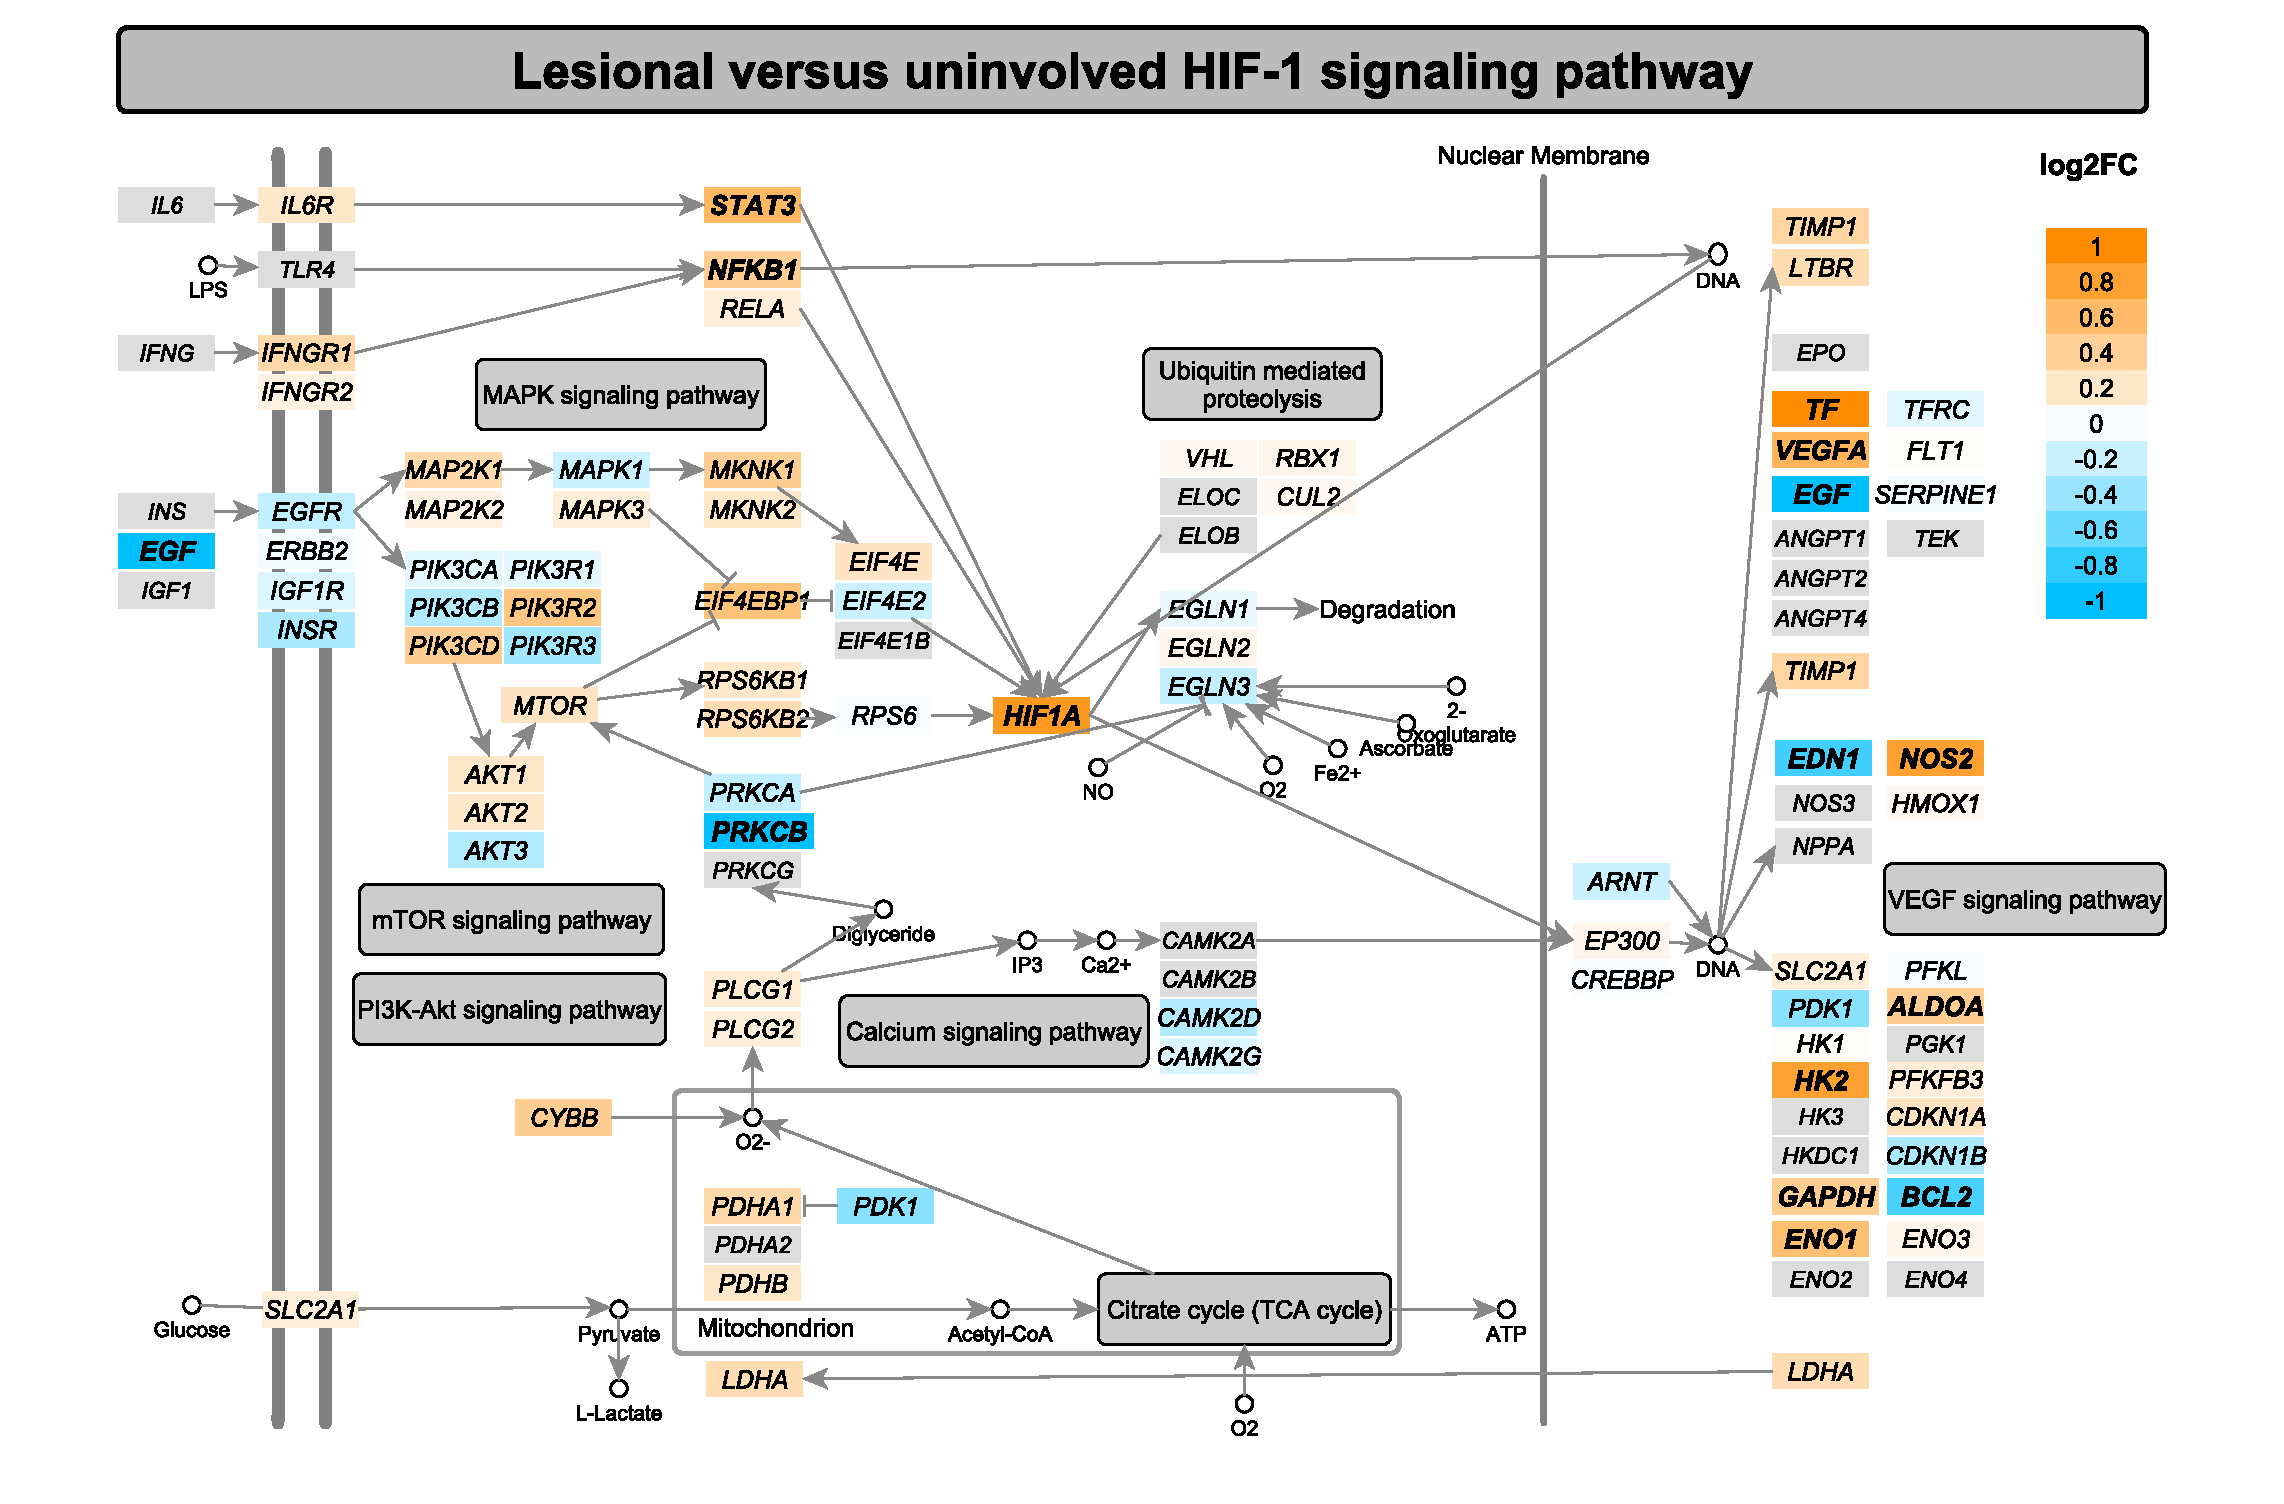
\includegraphics[width=0.9\textwidth]{./Results2/pdfs/PS_lesional_uninvolved_all_HIF_1_pathway}
%\caption[Mapping of the DEGs between lesional and uninvolved epidermis from psoriasis patients onto the HIF-I signalling pathway.]{\textbf{Mapping of the DEGs between lesional and uninvolved epidermis from psoriasis patients onto the HIF-I signalling pathway.} This pathway was sourced from KEGG, manually curated in a way that all member genes are maximised visually and then automatically color-coded by the log$_2$fold change expression between the lesional and uninvolved epidermis. Significant DEGs (FDR$<$0.05) are highlighted in bold. This pathway was identified by enrichment analysis using only DEGs (FDR$<$0.05).}
%\label{figure:PS_lesional_vs_uninvolved_HIF_pathway}
%\end{figure}



\begin{figure}[htbp]
	\centering
	\begin{subfigure}{0.8\textwidth}
		\centering
		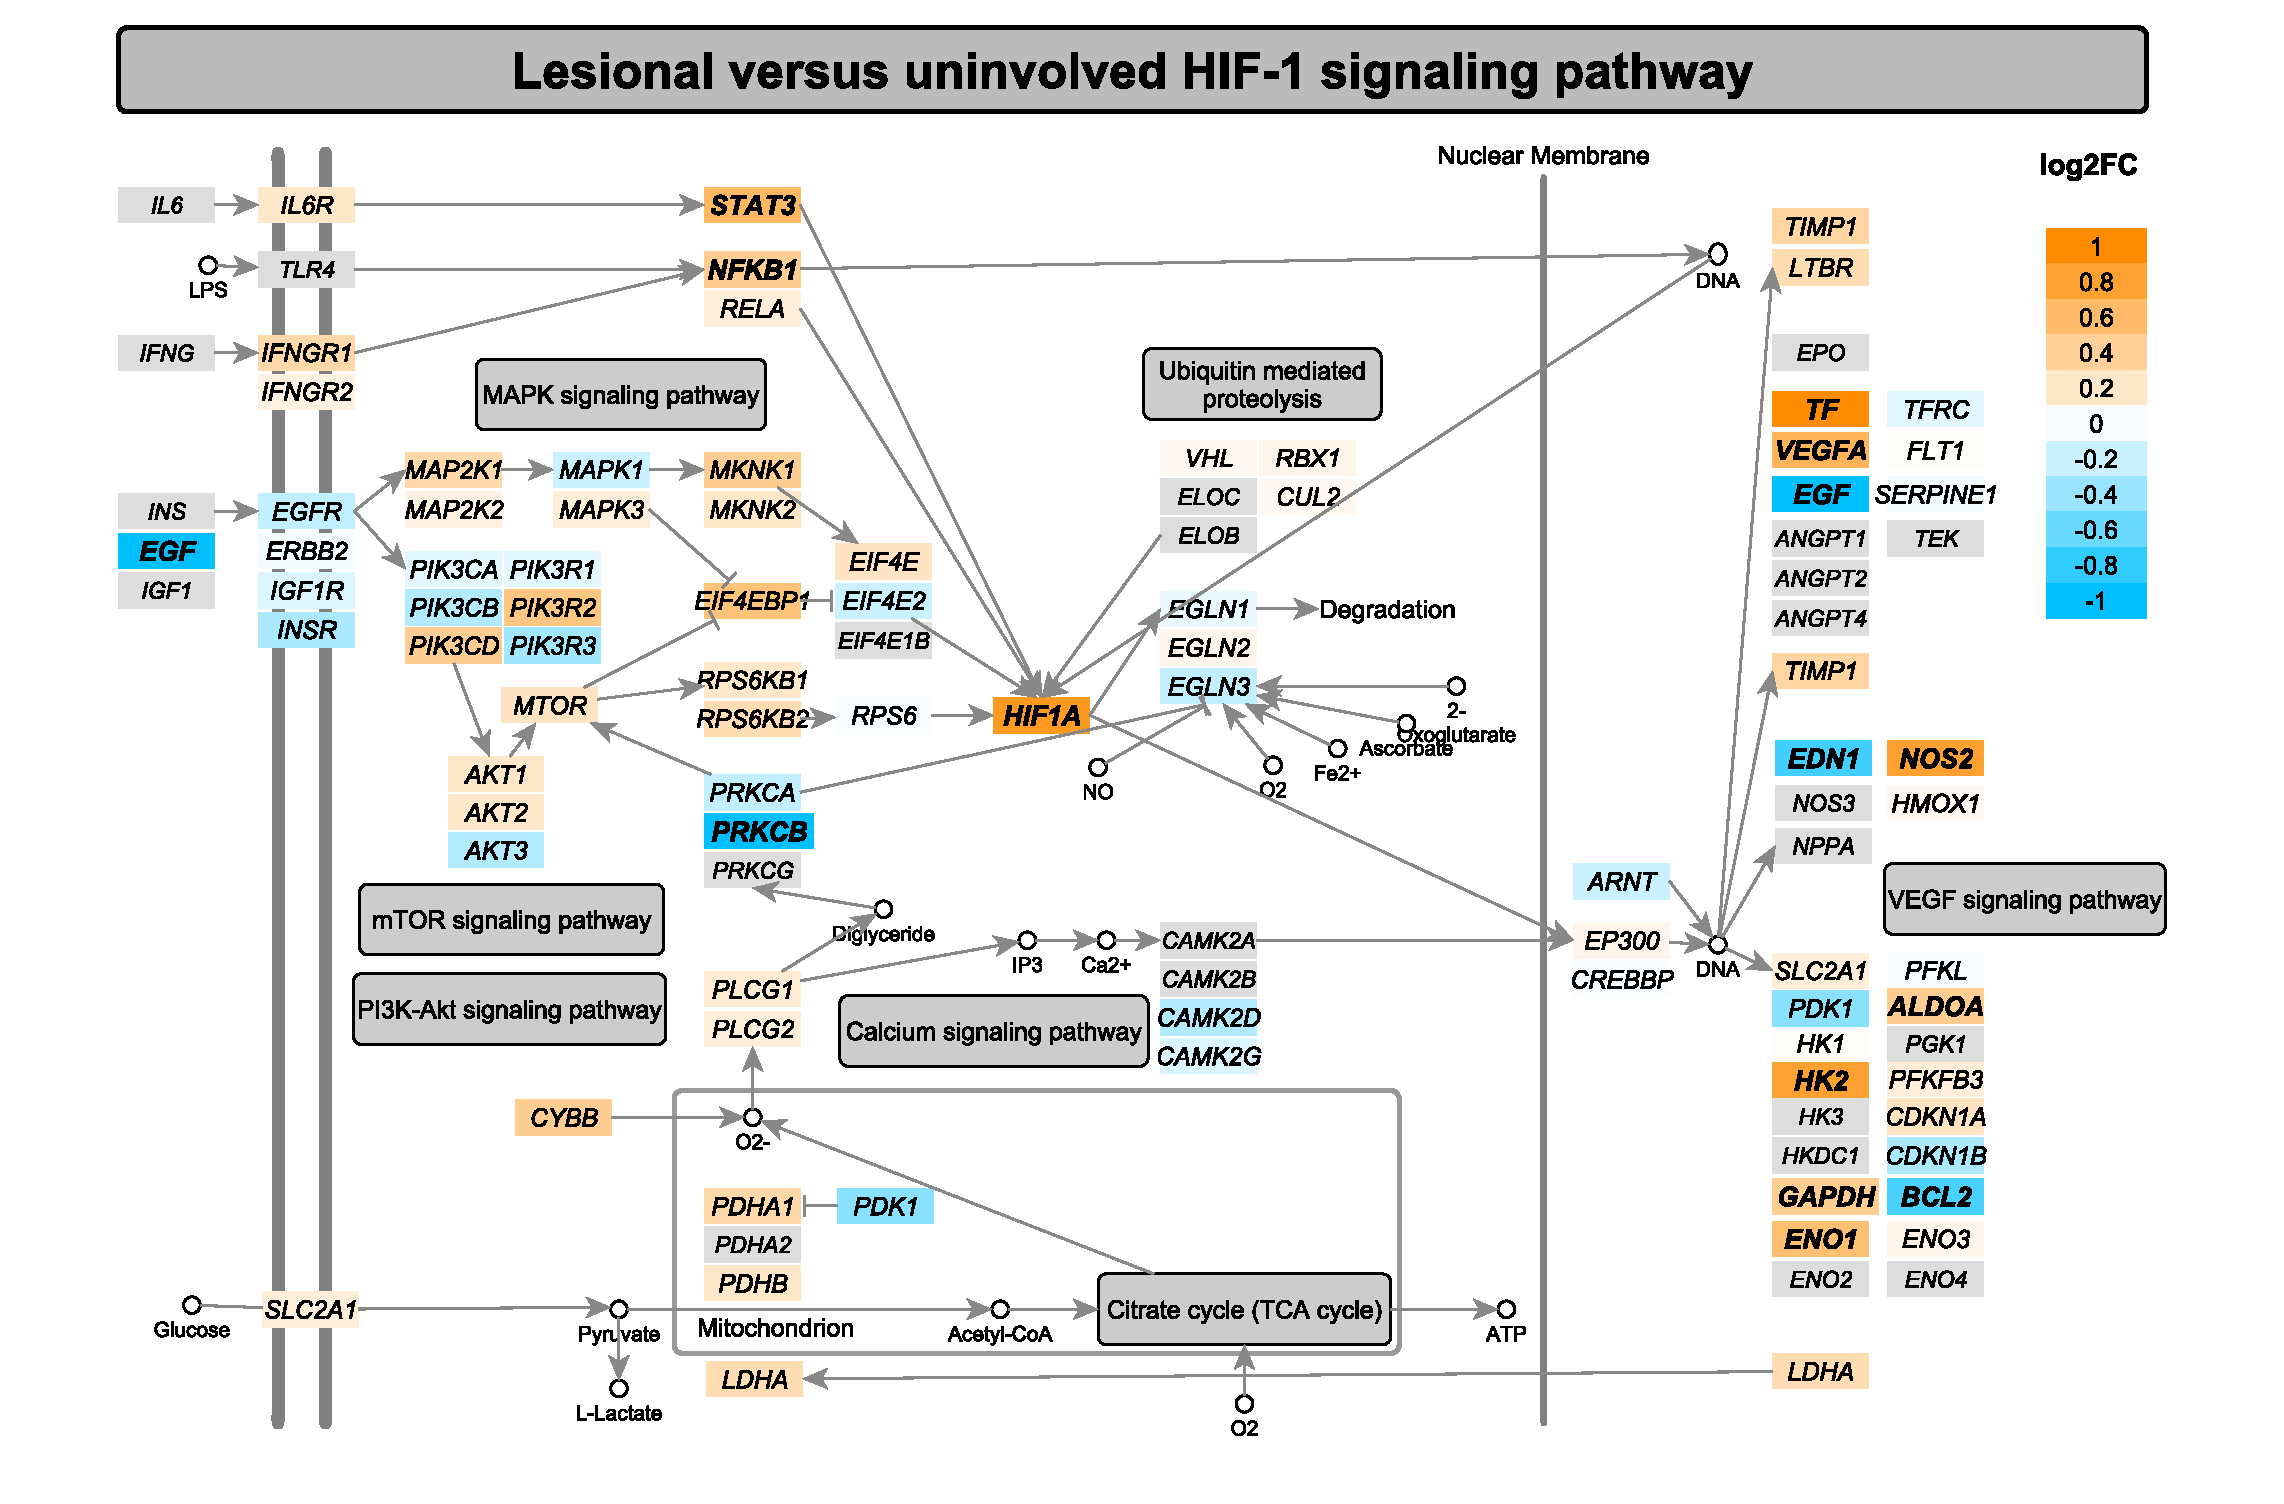
\includegraphics[width=\textwidth]{./Results2/pdfs/PS_lesional_uninvolved_all_HIF_1_pathway}
		\caption{\textbf{}}
		% The percentage sign indicated that the other subfig goes side by side
	\end{subfigure}
	\begin{subfigure}{0.8 \textwidth}
		\centering
		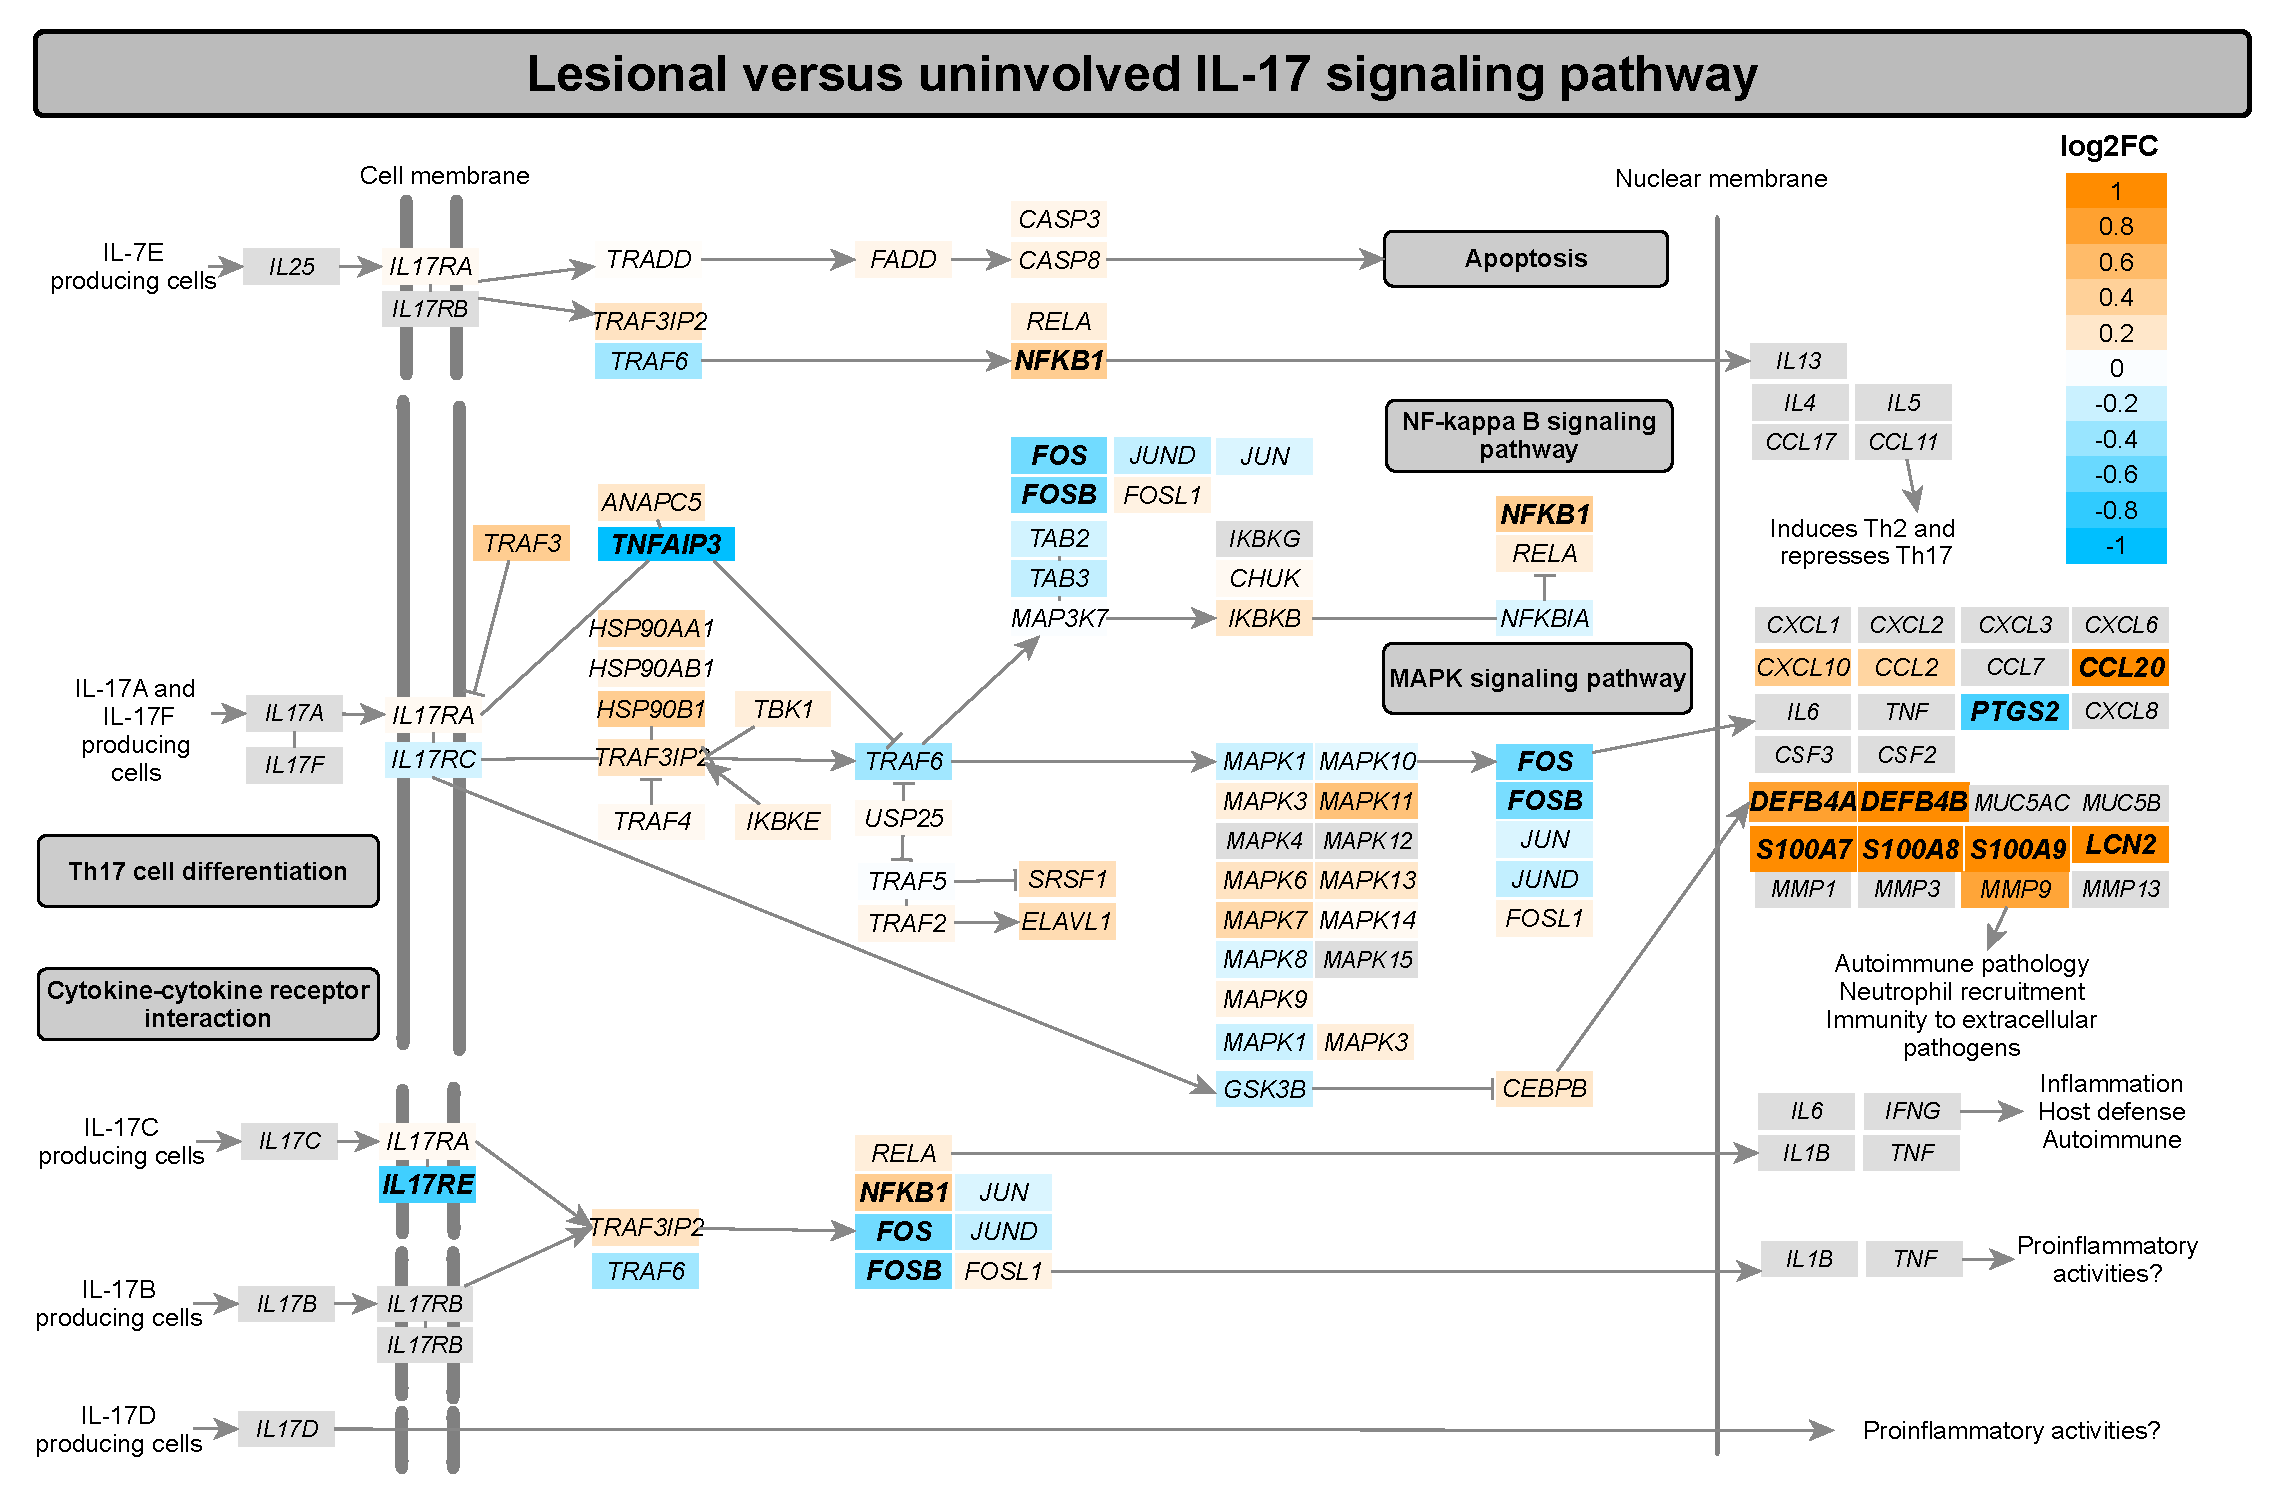
\includegraphics[width=\textwidth]{./Results2/pdfs/PS_lesional_uninvolved_all_IL17_pathway}
		\caption{\textbf{}}
	\end{subfigure}
\caption[Mapping of the DEGs between lesional and uninvolved epidermis from psoriasis patients onto the HIF-1 and IL-17 signalling pathways.]{\textbf{Mapping of the DEGs between lesional and uninvolved epidermis from psoriasis patients onto the HIF-1 and IL-17 signalling pathways.} The (A) HIF-1 and (B) IL-17 signalling pathways were sourced from KEGG, manually curated in a way that all member genes are maximised visually and then automatically color-coded by the log$_2$fold change expression between the lesional and uninvolved epidermis. Significant DEGs (FDR$<$0.05) are highlighted in bold. These pathways were identified by enrichment analysis using DEGs FDR$<$0.05.}
\label{figure:PS_lesional_vs_uninvolved_HIF_IL17_pathway}
\end{figure}


Immune relevant pathways including IFN, IL-17 and NOD-like receptor signalling were also identified in this analysis. The NOD-like receptor pathway was enriched with 23 significantly DEGs and it is involved in pathogen recognition and generation of an innate immune responses through activation of the inflammasome or through NF-$\kappa$B and MAPK with subsequent cytokine production and apoptosis.  %This pathway has also been identified as one of the most significantly enriched for DEGs in the epidermal study of Tervaniemi and colleagues.  
This included up-regulation of \textit{NOD2}, \textit{CARD6},  \textit{IFI16}, \textit{NLRX1}, \textit{IRF7} and \textit{NFKB1} (Figure \ref{figure:PS_lesional_vs_uninvolved_NOD_pathway} in orange and bold) and down-regulation of \textit{TNFAIP3}, \textit{TXNIP} and \textit{BCL-2} (Figure \ref{figure:PS_lesional_vs_uninvolved_NOD_pathway} in blue and bold), amongst others. % amongst others, and they were also up-regulated in Tervaniemi's data, where 42 DEGs mapped to this pathway. Amongst the down-regulated genes contributing to this pathway were \textit{TNFAIP3} and \textit{BCL-2} (Figure \ref{figure:PS_lesional_vs_uninvolved_NOD_pathway} in blue and bold). Performing pathway enrichment analysis using the DEGs from Tsoi and colleagues failed to show significant enrichment for NOD-like receptors signalling (19 DEGs in the NOD-like pathway). Nevertheless, NOD-like receptors signalling remained significantly enriched (13 DEGs mapping to this pathway) when the analysis was conducted using only the DEGs from the in-house data not overlapping the Tsoi and colleagues results. 
%These findings highlight the failure of whole skin biopsies transcriptomics to identify additional NOD-I signalling genes differentially regulated between lesional and uninvolved skin and the value of studying epidermal biopsies to unveil exacerbated dysregulation of functional pathways in KCs.

Another relevant pathway enriched in DEGs between lesional and uninvolved epidermis was IL-17 signalling. Enrichment of this pathways was driven by up-regulation of the S100 protein family (\textit{S100A7}, \textit{S100A8} and \textit{S100A9}) and chemokines such as \textit{CCL20}, which binds the receptor CCR6 and is involved in DCs and T cell chemotaxis (Figure \ref{figure:PS_lesional_vs_uninvolved_HIF_IL17_pathway}B in orange and bold). Notably, \textit{IL17RE} which together with IL-17RA forms the receptor for IL-17C was down-regulated in lesional skin (Figure \ref{figure:PS_lesional_vs_uninvolved_HIF_IL17_pathway}B in blue and bold). 

\begin{landscape}
\begin{figure}[htbp]
\centering
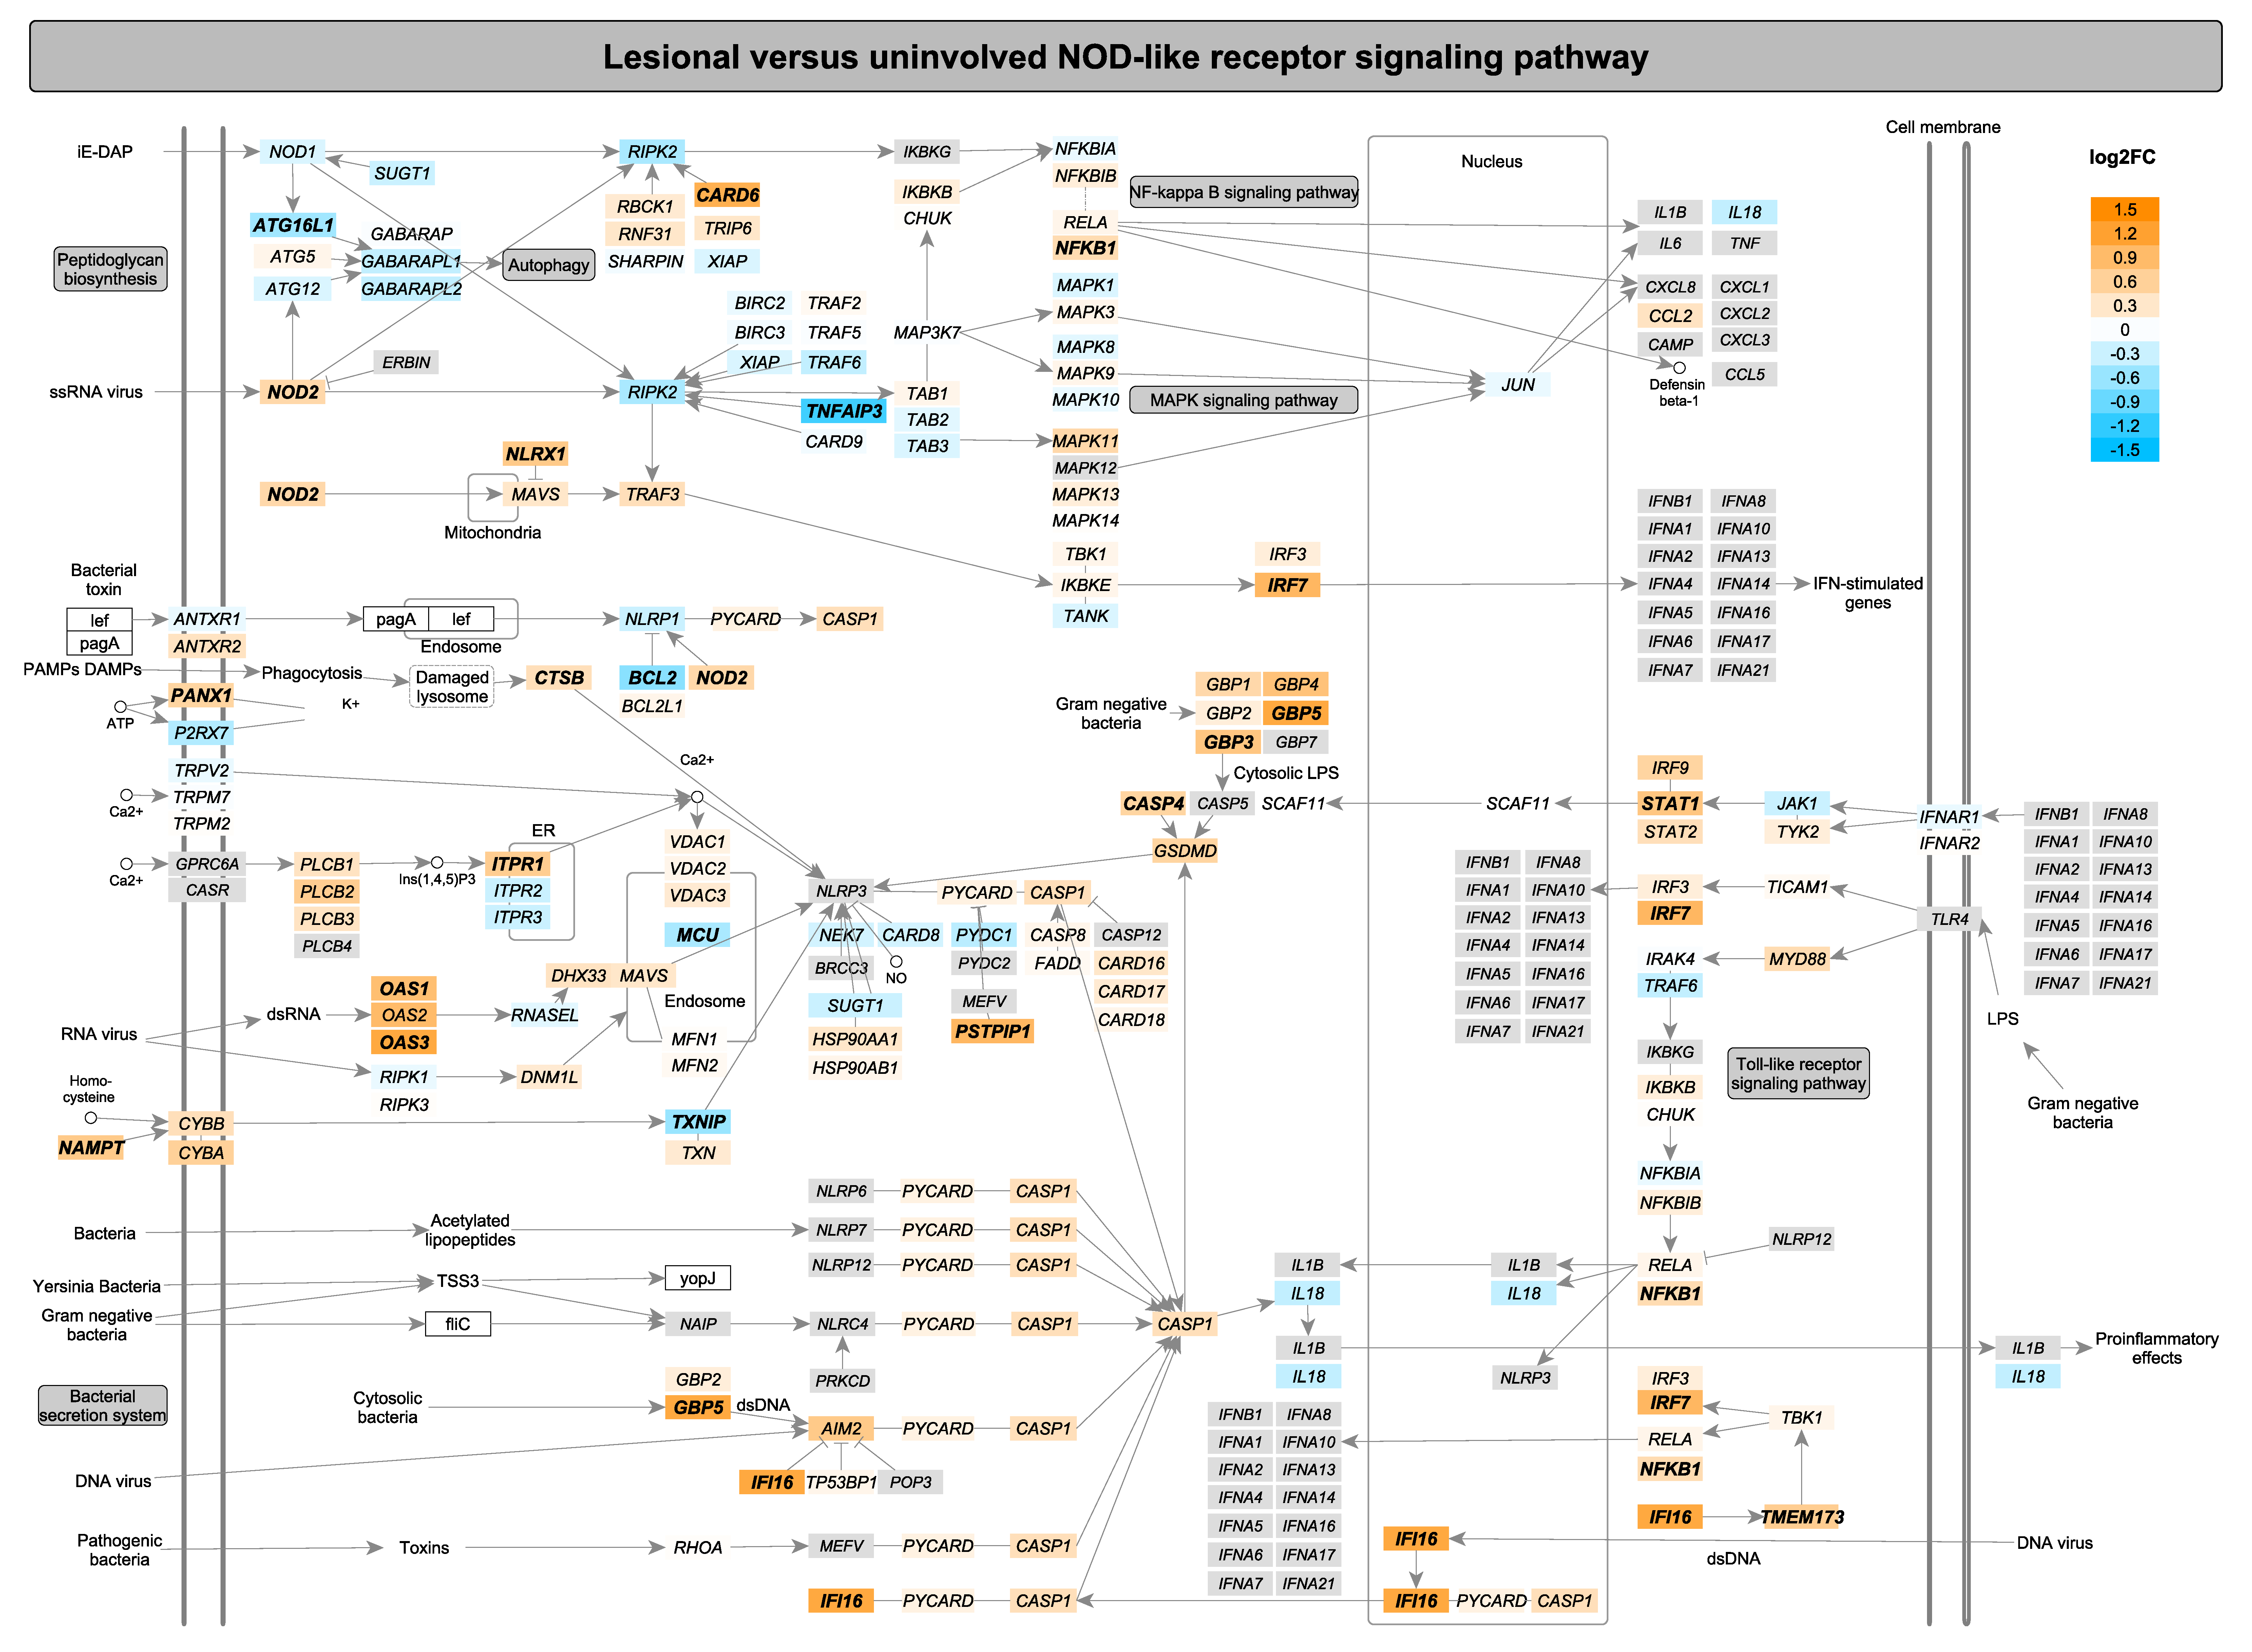
\includegraphics[width=\textwidth]{./Results2/pdfs/PS_lesional_uninvolved_all_NOD_like_pathway}
\caption[Mapping of the DEGs between lesional and uninvolved epidermis from psoriasis patients onto the NOD-like signalling pathway.]{\textbf{Mapping of the DEGs between lesional and uninvolved epidermis from psoriasis patients onto the NOD-like signalling pathway.} This pathway was sourced from KEGG, manually curated in a way that all member genes are maximised visually and then automatically color-coded by the log$_2$fold change expression between the lesional and uninvolved epidermis. Significant DEGs (FDR$<$0.05) are highlighted in bold. This pathway was identified by pathway enrichment analysis using only DEGs (FDR$<$0.05).}
\label{figure:PS_lesional_vs_uninvolved_NOD_pathway}
\end{figure}
\end{landscape}


\noindent Enrichment of DEGs between lesional and uninvolved skin for the peroxisome proliferator-activated receptor (PPAR) signalling and AGE-RAGE signalling in diabetic complications highlighted the link between metabolic dysregulation (particularly oxidation of lipids, carbohydrates and aminocacids) and immunity. PPAR signalling involved up-regulation of the PPAR receptor $\delta$ (\textit{PPARD}) (fold change=1.39), the stearoyl-CoA desaturase \textit{SCD} (fold change=1.82), involved in fatty acid synthesis, and \textit{CD36} (fold change=2.44), a fatty acid transport, all of them DEGs in the Tsoi and Tervaniemi studies.

%contributing to the psoriasis pathophysiology and increased risk of co-morbidities, such as metabolic syndrome and CVD. 

%PPARs are ligand-dependent TF that have been shown to induce the inhibition of pro-inflammatory genes including IL-1 and TNF-$\alpha$ \parencite{Ji2001}. In skin, PPARs have been demonstrated to contribute to homeostasis by inducing differentiation and preventing proliferation \parencite{Rivier1998}. Moreover, inhibition of genes regulated by PPAR-$\gamma$ has been described in studies comparing lesional versus healthy skin biopsies \parencite{Li2014}.
%CCL20 https://www.ncbi.nlm.nih.gov/pubmed/19295614
%CCR6-CCL20 Dendritic Cells Rapidly Recruited into Epithelial Tissues via CCR6/CCL20 Are Responsible for CD8+ T Cell Crosspriming In Vivo

%Also sharing ECM, cell junctions and pathwsys in cancer, in our case microRNAs.


\subsection{Comparison of systemic and tissue specific gene expression signatures in psoriasis}

In order to investigate commonalities and differences in psoriasis gene expression in the affected tissue (skin) and at the systemic level (circulating immune cells), overlap between the lists of DEGs was performed. Only modest overlap was found between DEGs in lesional skin compared to uninvolved and the DEGs identified in circulating immune cells. CD14$^+$ monocytes and CD8$^+$ cells showed the greatest overlap; however many of these genes did not show a consistent direction of change in differential expression (Table \ref{tab:RNAseq_overlap_circulating_versus_skin}). Examples included \textit{TNFAIP3}, which was up-regulated in psoriasis CD4$^+$ and CD8$^+$ cells compared to controls but down-regulated in lesional epidermis in comparison to uninvolved. Similarly, early growth response genes were up-regulated in CD14$^+$ monocytes (\textit{EGR3}) and CD4$^+$ T cells (\textit{EGR1}, \textit{EGR2} and \textit{EGR3}) but showed down-regulation (\textit{EGR2} and \textit{EGR3}) in lesional epidermis compared to uninvolved.  
%A similar or larger proportion of the total overlapping DEGs presented opposite direction of change in circulating immune cells and in skin from psoriasis patients. An examples was \textit{TNFAIP3} gene, which was up-regulated in psoriasis CD4$^+$ and CD8$^+$ cells compared to controls and down-regulated in lesional epidermis when compared to uninvolved.  
%In Tsoi \textit{et al.}, 2015 this gene did not change expression between lesional and uninvolved nor between lesional and healthy skin and Li \textit{et al.}, reported its up-regulation in lesional skin. 
%Interestingly, no overlap was observed for genes of the \textit{S100} family, only found to be up-regulated in lesional skin. Lastly, the previously described \textit{MIR146A} also appeared dysregulated in opposite direction in CD8$^+$ cells and in the skin analysis, presenting down- and up-regulation, respectively.

Examples of genes changing in the same direction in immune-cells and psoriasis skin included the up-regulation in CD14$^+$ monocytes of the nicotinamide phosphoribosyltransferase involved in stress response and inflammation \textit{NAMPT} \parencite{Presumey2013} and the down-regulation in CD8$^+$ cells of the protein kinase \textit{PRKCB}.
 
%EGR2 and 3 https://www.ncbi.nlm.nih.gov/pmc/articles/PMC3477314/

\begin{table}[htbp]
%\setlength{\tabcolsep}{20pt} only to stretch the columns if you want
%\renewcommand{\arraystretch}{1.5}
\centering
\begin{tabular}{@{} c c c c}
\toprule
\textbf{DEGs overlapping}   & \textbf{Total overlap}   & \textbf{Same direction}  & \textbf{Opposite direction}\\
\textbf{with skin}          &                          &                          &                            \\
\midrule 
\midrule
CD14$^+$ monocytes          & 37                       & 19                       &  18                         \\ 
CD4$^+$                     & 10                       & 6                        &  4                           \\
CD8$^+$                     & 37                       & 24                       &  13                           \\
CD19$^+$                    & 16                       & 5                        &  11                          \\
\bottomrule 
\end{tabular}
\medskip %gap
\caption[Overlap between the DEGs in the four circulating immune cell types (psoriasis patients vs controls) and the DEGs in psoriasis patients skin biopsies (lesional vs uninvolved).]{\textbf{Overlap between the DEGs in the four circulating immune cell types (psoriasis patients vs controls) and the DEGs in psoriasis patients skin biopsies (lesional vs uninvolved).} DEGs based on FDR$<$0.05 for each of the comparisons} 
\label{tab:RNAseq_overlap_circulating_versus_skin}
\end{table}
\bigskip %bigger spac

%Talk about NOD genes overlapping the circulation DEGs
%Mention about IFN pathway

The limited overlap between circulating and skin DEGs was also reflected in the different enriched pathways identified for each analysis. CD14$^+$ and CD8$^+$ DEGs were mostly enriched for immune-related pathways, including TCR , IL-12 , TNF and NF-$\kappa$B signalling, and no enrichment was found for metabolic, oxidative stress and cell cycle, which showed significant dysregulation in skin. %Moreover,some of the pro-inflammatory genes contributing to those pathways appeared down-regulated in psoriasis when compared to controls, as previously commented.% some of the genes in these circulating immune cells suggested certain immuno-supression features that could be characteristic of these cells before or/and after having been exposed to the skin inflammatory \textit{milieu}. 
Moreover, the DEGs contributing to the enrichment of immune-related pathways in psoriatic epidermis had a more pronounced pro-inflammatory signature, consistent with the skin being the main site of active inflammation.


\subsection{Integration of chromatin accessibility and expression data for peripheral blood immune cells in psoriasis}
The characterisation of the chromatin accessibility landscape and the transcriptome of circulating immune cells from psoriasis patients revealed a greater effect of disease status on gene expression than in chromatin accessibility. An integrated analysis combining evidence of differential accessibility and expression in the four investigated immune cell types was performed by overlapping proximal genes to DARs ($<$5Kb) and DEGs. An overlap was only found in CD8$^+$ cells, where 6 out of the 53 DARs colocalised with DEGs in this cell type (\textit{ARL4A}, \textit{ASCL2}, \textit{ENTPD1}, \textit{TIAM1}, \textit{TRAT1} and \textit{ZNF276}).

An example was T Cell lymphoma invasion and metastasis 1 (\textit{TIAM1}), which activates IL-17 expression and T cell transendothelial migration during inflammation \parencite{Kurdi2016, Gerard2009} an was up-regulated (log$_2$fold change 0.44) in CD8$^+$ cells from psoriasis patients (Figure \ref{figure:ATAC_RNAseq_CD8_TIAM1_TRAT1}A). Likewise, psoriasis CD8$^+$ cells presented greater chromatin accessibility compared to healthy controls (log$_2$fold change 0.41) in a region located in an intron of \textit{TIAM1} annotated as an active enhancer according to the chromatin segmentation data in this cell type (Figure \ref{figure:ATAC_RNAseq_CD8_TIAM1_TRAT1}C). Common SNPs within this DAR were not identified as eQTLs in CD8$^+$ cells \parencite{Kasela2017}; however promoter capture Hi-C data in unstimulated CD8$^+$ cells revealed physical interaction between this region and the promoter of \textit{TIAM1} \parencite{Javierre2016}. 

Another two relevant genes in the immune response with overlapping ATAC and RNA-seq were the ectonucleoside triphosphate diphosphohydrolase 1 (\textit{ENTPD1}), which hydrolyses the pro-inflammatory mediator ATP attenuating the inflammation, and the TCR-associated transmembrane adaptor 1 (\textit{TRAT1}) gene, a positive regulator of TCR signalling \parencite{Antonioli2013, Valk2006}. Both, \textit{ENTPD1} and \textit{TRAT1}, showed up-regulated expression (Figure \ref{figure:ATAC_RNAseq_CD8_TIAM1_TRAT1}B) and increased chromatin accessibility (Figure \ref{figure:ATAC_RNAseq_CD8_TIAM1_TRAT1}D) in psoriasis patients CD8$^+$ cells compared to healthy controls.

% mention about TIAM1 being a good target in Pi
%short check for the ENTPD1 and TRAT1 DARs to be likely to affect 
\begin{figure}[htbp]
\centering
\begin{subfigure}{0.5\textwidth}
\centering
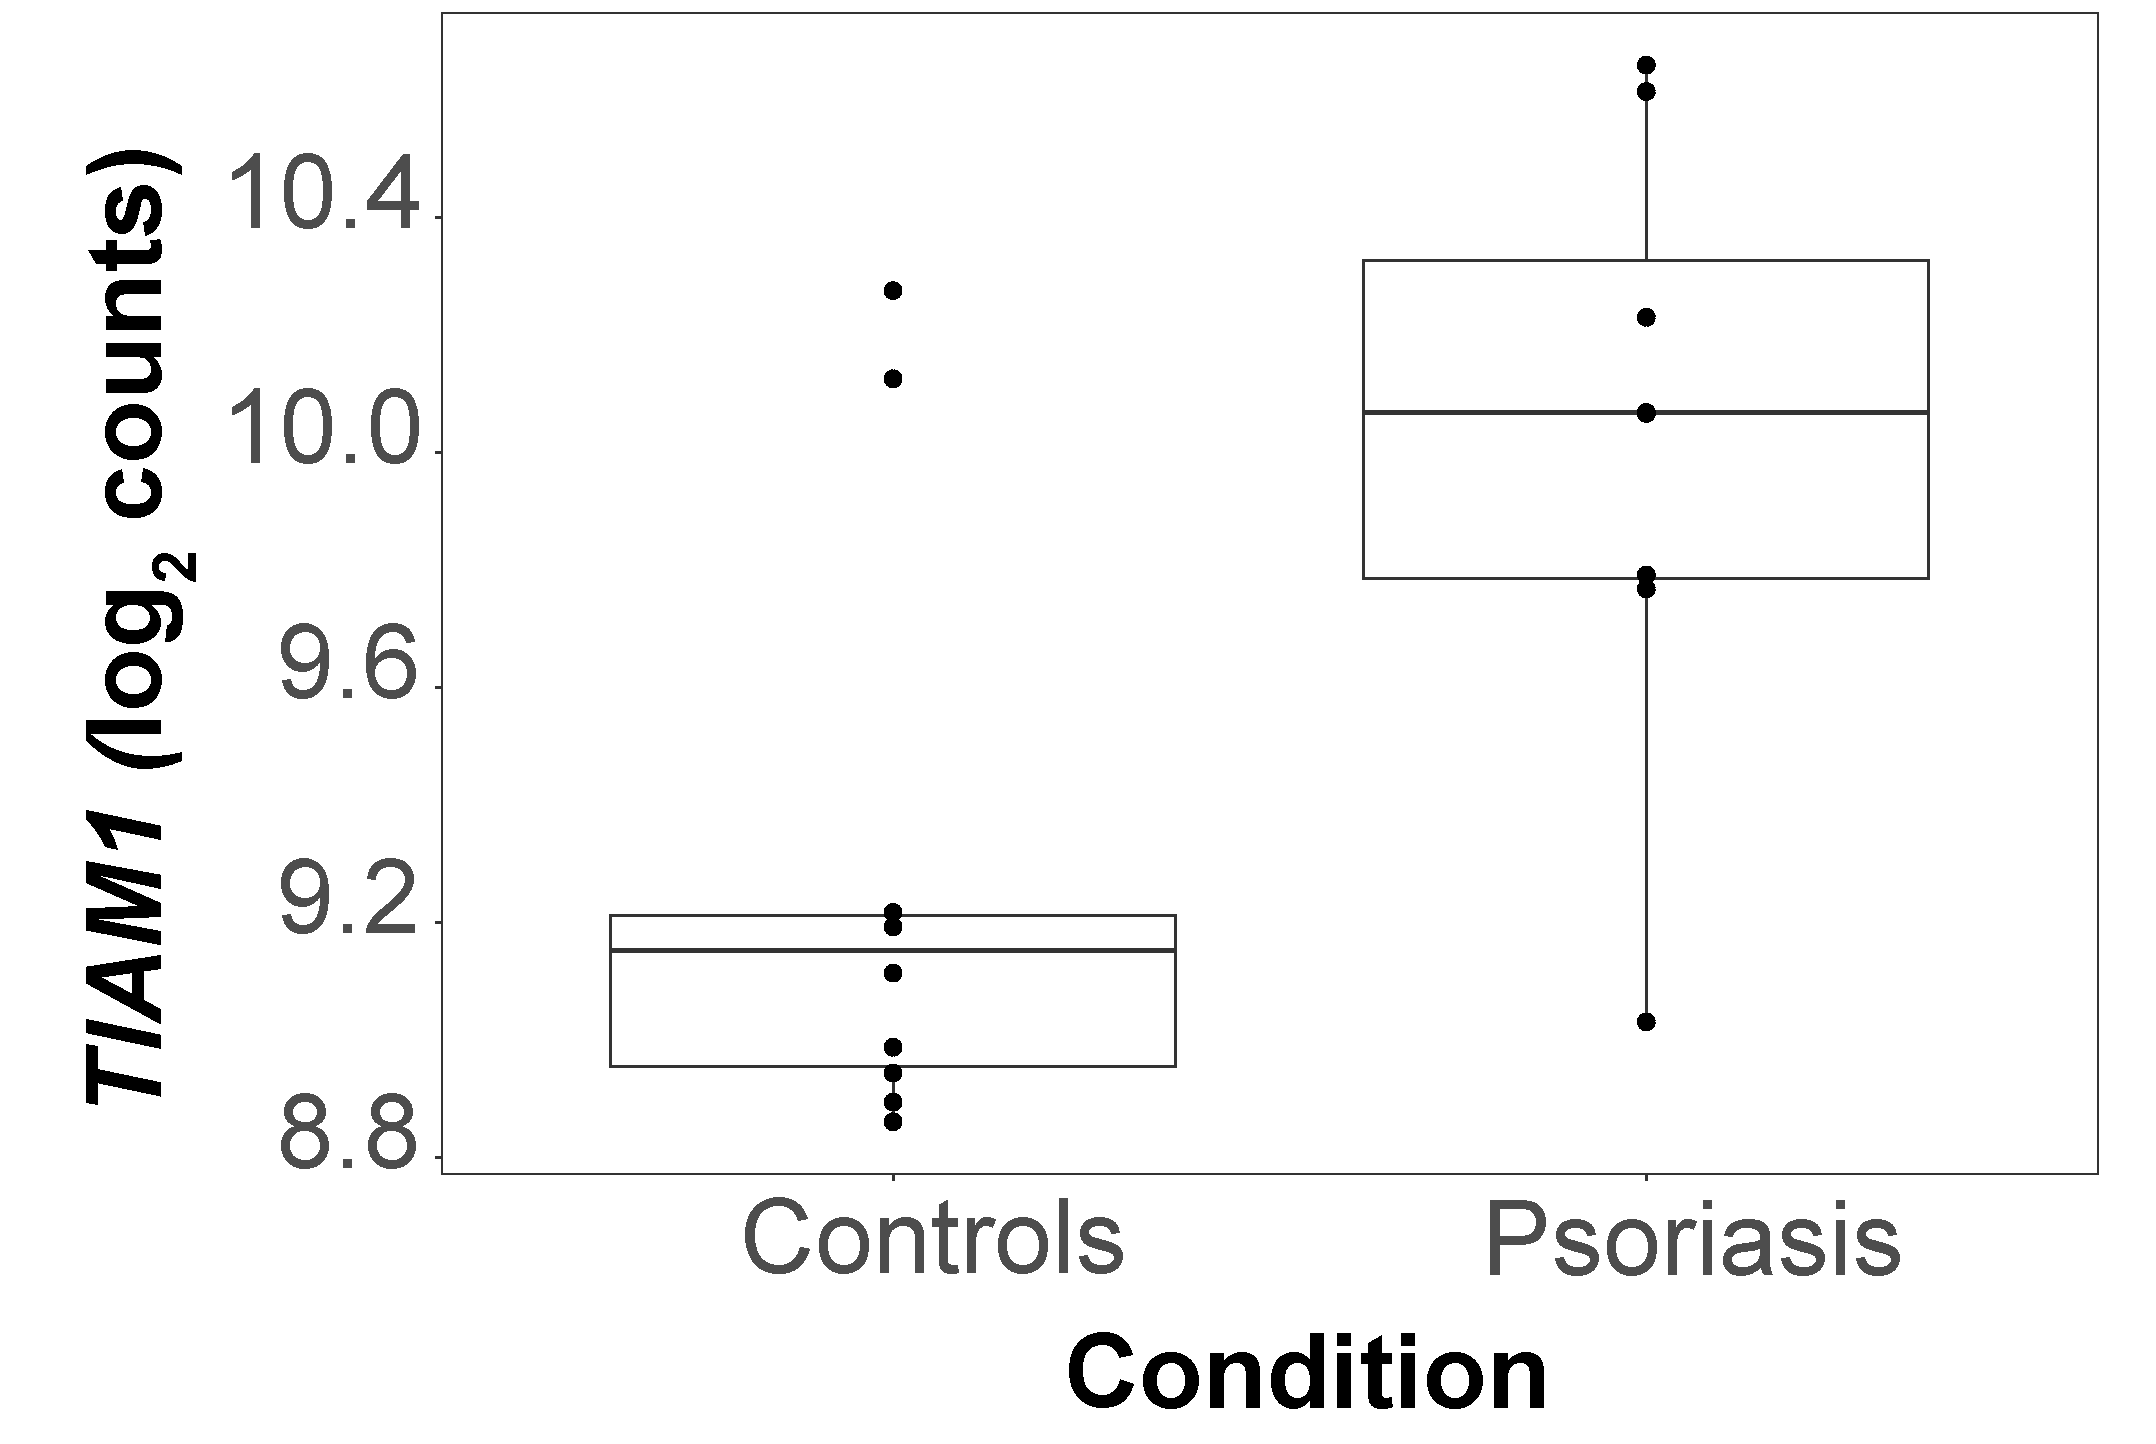
\includegraphics[width=\textwidth]{./Results2/pdfs/RNAseq_ATAC_TIAM1_boxplot}
\caption{\textbf{}}
% The percentage sign indicated that the other subfig goes side by side
\end{subfigure}%
\begin{subfigure}{0.5\textwidth}
\centering
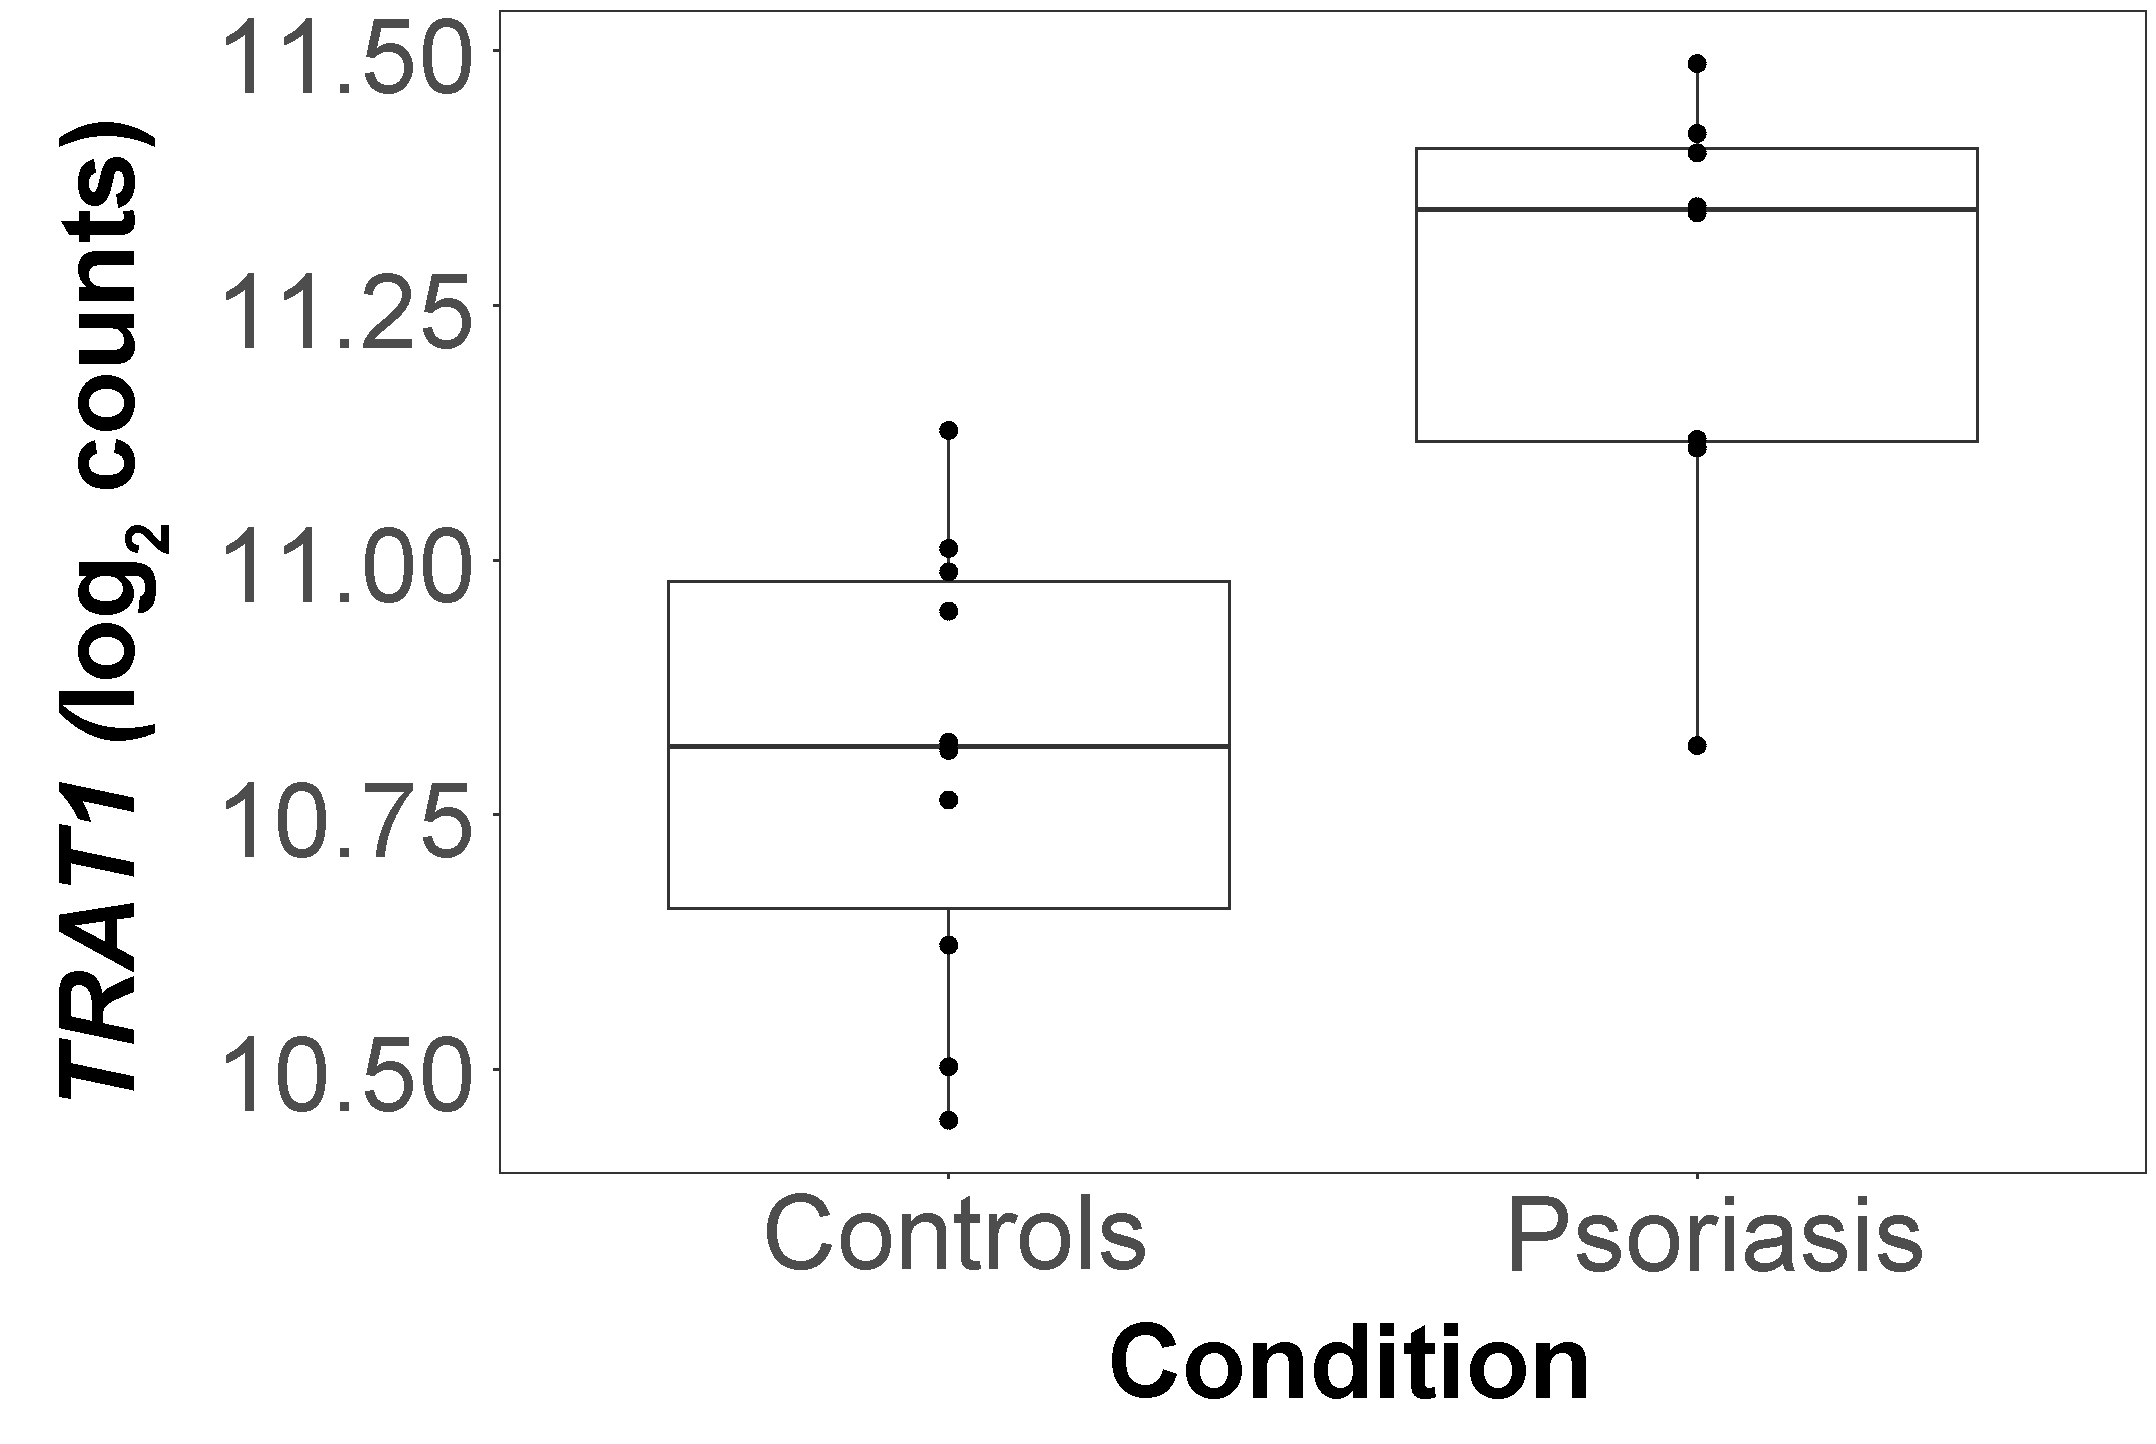
\includegraphics[width=\textwidth]{./Results2/pdfs/RNAseq_ATAC_TRAT1_boxplot}
\caption{\textbf{}}
\end{subfigure}
\begin{subfigure}{0.45\textwidth}
\centering
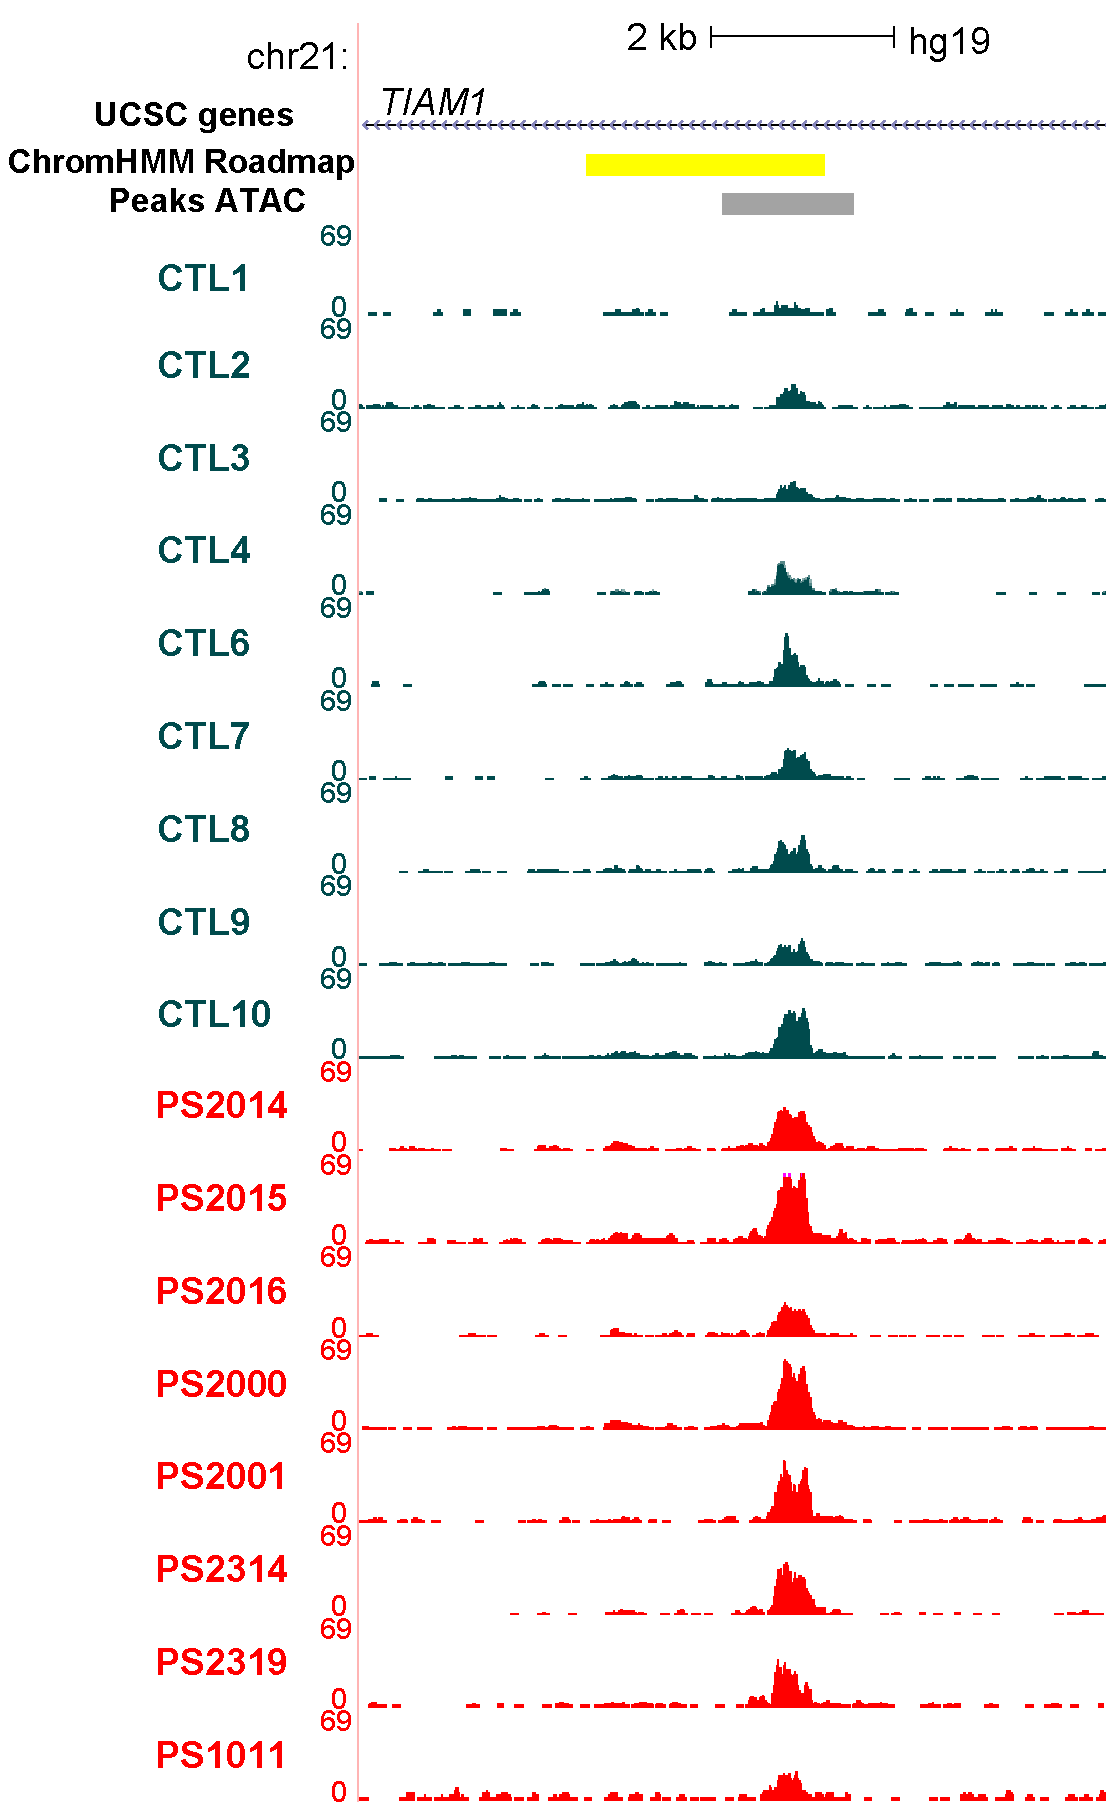
\includegraphics[width=\textwidth]{./Results2/pdfs/ATAC_CD8_peak_TIAM1_track}
\caption{\textbf{}}
% The percentage sign indicated that the other subfig goes side by side
\end{subfigure}%
\begin{subfigure}{0.45\textwidth}
\centering
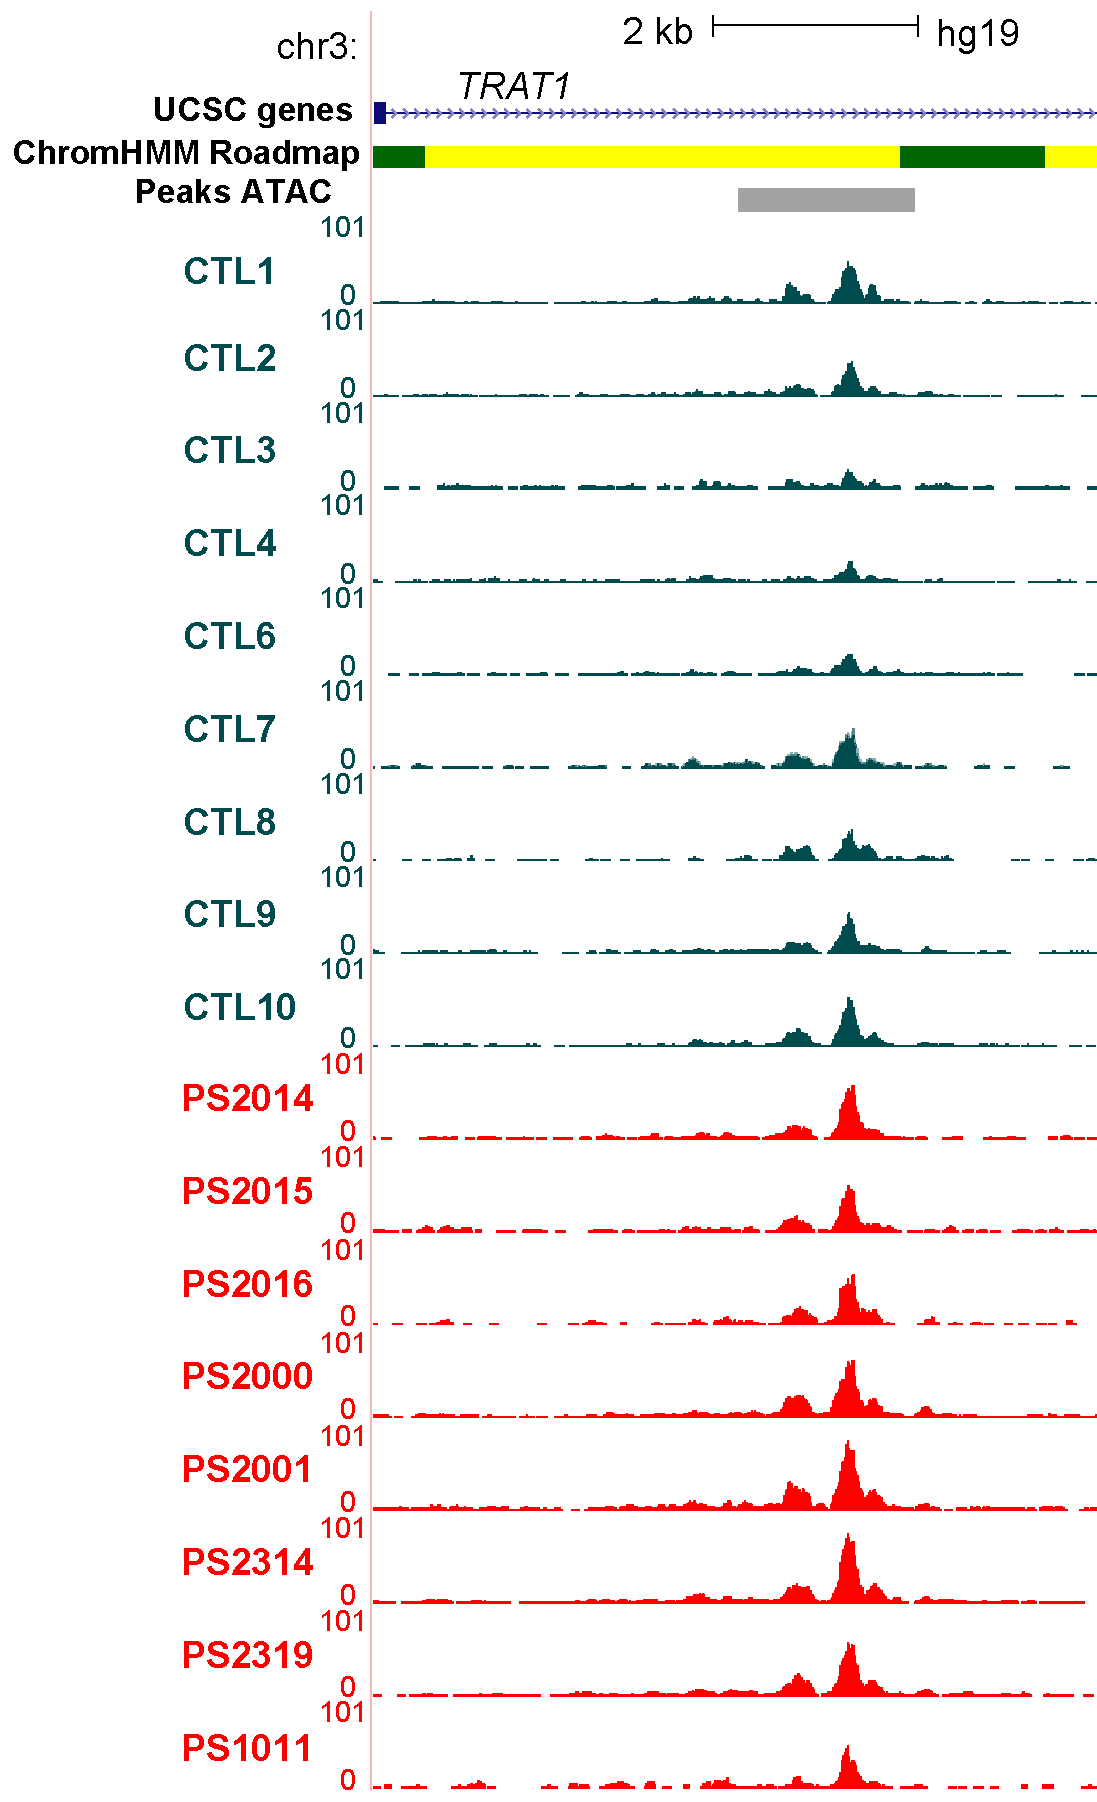
\includegraphics[width=\textwidth]{./Results2/pdfs/ATAC_CD8_peak_TRAT1_RNA_overlap}
\caption{\textbf{}}
\end{subfigure}
\caption[Differential gene expression and chromatin accessibility landscape for \textit{TIAM1} and \textit{TRAT1} genes in CD8$^+$ cells.]{\textbf{Differential gene expression and chromatin accessibility landscape for \textit{TIAM1} and \textit{TRAT1} genes in CD8$^+$ cells.} Boxplots show RNA-seq log$_{2}$ normalised counts for (A) \textit{TIAM1} and (B) \textit{TRAT1} in psoriasis and healthy controls CD8$^+$ cells. UCSC Genome Browser view illustrating the normalised ATAC read density (y-axis) in introns of (C) \textit{TIAM1} and (D) \textit{TRAT1} genes (x-axis) in CD8$^+$ cells. Tracks are colour-coded by condition and assay: control (CTL)=dark turquoise and psoriasis (PS)=red. The Roadmap Epigenomics Project chromatin segmentation map for CD8$^+$ cells is shown above the ATAC tracks.}
\label{figure:ATAC_RNAseq_CD8_TIAM1_TRAT1}
\end{figure}



\subsection{Fine-mapping of psoriasis GWAS loci and functional interpretation}

\subsubsection{Fine-mapping using summary statistics data}
Due to the impossibility of accessing genotyping data, fine-mapping of psoriasis Immunochip GWAS loci was conducted using summary statistics of the Immunochip psoriasis GWAS study from Tsoi \textit{et al.} 2012. This study was based on two cohorts (GAPC and PAGE) and only summary statistics for the GAPC cohort (2,997 cases and 9,183 controls) were publicly available in ImmunoBase at the time of this analysis. As explained in Chapter \ref{ch:Mat}, fine-mapping from summary statistics with DIST used the z-score statistics of each of the genotyped SNPs from the GAPC cohort to impute the z-scores for the missing SNPs based on the r$^2$ relationship from the 1000 Genome Project Version 3 \parencite{Lee2013}. Following z-score imputation for the non-genotyped SNPs, association analysis was performed and ABF, PP and credible set of SNPs were built for each GWAS signal (Tables \ref{tab:Psoriasis_fine_mapping_summary}).

Fine-mapping was performed for 25 of the Immunochip psoriasis GWAS loci reported by Tsoi \textit{et al.} 2012, excluding the MHC and those loci which lead SNPS were in high LD with missense mutations having experimentally proved or highly confident predicted damaging effects. Out of the 25 regions, 8 loci did not reach log$_{10}$ABF$>$3 (cut-off used as in Bunt \textit{et al.} 2015) with 90\% credible sets ranging from 19 to 853 SNPs (Table \ref{tab:Psoriasis_fine_mapping_summary} bottom). In 10 loci presenting log$_{10}$ABF$>$3, the fine-mapping lead SNP was in low LD with the Tsoi \textit{et al.} 2012 GWAS lead SNP and/or was not included in the 90 or 50\% credible set (Table \ref{tab:Psoriasis_fine_mapping_summary} with $^\ast$). This is likely due to the lack of power as only summary statistics from one cohort were available for this analysis.


\begin{landscape}
\renewcommand{\arraystretch}{0.7}
\begin{center}
%\begin{longtable}[ht]{p{.25\textheight} p{.40\textheight} p{.25\textheight} p{.60\textheight}}
\begin{longtable}[ht]{c c c c c c c c c c c}
\caption[Summary results for the fine-mapping analysis of 26 psoriasis Immunochip GWAS loci.]{\textbf{Summary results for the fine-mapping analysis of 26 psoriasis Immunochip GWAS loci.} For the 17 Immunochip psoriasis GWAS loci showing log${_10}$ABF$>3$, the table reports the closer gene(s), FM lead SNP, RAF, imputation status, z-score, OR for the GAPC cohort lead SNP, log$_{10}$ABF for the FM lead SNP, PP, number of SNPs included in the 90\% credible set and the Tsoi \textit{et al.} 2012 GWAS lead SNP. Imputation status refers to whether the SNP was imputed (Yes) or genotyped by the Immunochip array (No). If a SNP is imputed, the z-score statistic was determined by imputation based on LD with other SNPs, as previously explained. The sign of the z-score indicates whether the RAF allele increases (+) or decreases (-) risk of psoriasis. In 10 of the loci with log$_{10}$ABF$\geq$3, the fine-mapping lead SNP was in low LD (r${^2}<0.5$) with the psoriasis GWAS SNP and did not contain it that SNP in the credible set (labelled with $^{\ast}$). Details of the 8 loci presenting log${_10}$ABF$<3$ are also included. FM=fine-mapping; RAF= reference panel allele frequency; OR=odds ratio; ABF=approximate Bayes factor; PP=posterior probability.}
\label{tab:Psoriasis_fine_mapping_summary} \\
\toprule
\textbf{chr} & \textbf{Closest} & \textbf{FM} & \textbf{RAF} & \textbf{Imputed}& \textbf{z} &\textbf{OR} & \textbf{log$_{10}$ABF} & \textbf{PP} & \textbf{90\% credible} &\textbf{Tsoi} \\
              & \textbf{gene} & \textbf{lead SNP} &        &                  &           &\textbf{GAPC} & \textbf{FM lead SNP} &             & \textbf{set}           &\textbf{lead SNP} \\
\midrule
\midrule
1	& \textit{IL28RA}&	     rs61774731$^{\ast}$   &		0.10 &	No	& -7.68 &1.21 &		11.5 &		0.99 &		1	 &	rs7552167 \\
2	& \textit{FLJ16341/REL}& rs6714339$^{\ast}$    &		0.14 &	No	& -6.82 &1.17 &		9.0  &		0.99 &		1	 &	rs62149416 \\
2	& \textit{IFIH1}&		     rs2111485$^{\ast}$    &		0.59 &	No	& 5.94  &1.27 &		6.7  &		0.50 &		2	 &	rs17716942 \\
5	& \textit{TNIP1}&		     rs17728338            &		0.06 &	No	& 7.45  &1.59 &		10.6 &		0.40 &		6	 &	rs2233278 \\
5	& \textit{IL12B/ADRA1B}& rs12188300            &		0.05 &	No	& 7.71  &1.58 &		11.2 &		0.18 &		9	 &	rs12188300 \\
6	& \textit{TNFAIP3}&		   rs1416173$^{\ast}$    &		0.85 &	No	& -6.36 &1.23 &		7.7  &		0.15 &		10 &		rs582757 \\
14	& \textit{NFKBIA}&		 rs74243591            &		0.21 &	No	& -5.23 &1.16 &		5.0  &		0.30 &		12 &		rs8016947 \\
17	& \textit{NOS2}&		   rs117094752$^{\ast}$  &		0.02 &	No  & -6.53 &1.22 &		7.3  &		0.94 &		1  &		rs28998802 \\
1	& \textit{SLC45A1/TNFRSF9}&		rs425371         &		0.25 &  Yes  & 5.52  &1.13 &		5.6  &		0.14 &		22 &		rs11121129 \\
1	& \textit{RUNX3}&		     rs61774731 $^{\ast}$  &		0.10 &	No	& -7.68 &1.13 &		11.5 &		0.99 &		1  &		rs7536201 \\
2	& \textit{B3GNT2/TMEM17}&rs9309343$^{\ast}$    &		0.33 &	Yes	& 4.92  &1.12 &		4.3  &		0.66 &		34 &		rs10865331 \\
  &  (2p15)               &                      &         &      &       &     &        &         &       &\\
7	& \textit{ELMO1}        &rs77840275$^{\ast}$   &		0.10 &	No	&-6.31  &1.11 &		7.5  &		0.99 &		1  &		rs2700987 \\
11	& \textit{ZC3H12C}    &rs11213274            &		0.40 &	Yes	& -4.78 &1.14 &		4.0  &		0.05 &		69 &		rs4561177 \\
11 & \textit{ETS1}	      & rs10893884	         &    0.53 &  No  & -4.51 &1.15 &  3.5	 &    0.26 &    19 &    rs3802826	 \\
16	& \textit{PRM3/SOCS1}& rs111251548$^{\ast}$  &		0.02 &	No	& -7.41 &1.13 &		9.4  &		0.97 &		1  &		rs367569 \\
17	& \textit{PTRF/STAT3}& rs963986              &		0.17 &	No	& 4.82  &1.15 &		4.1  &		0.18 &		8  &		rs963986 \\
19	& \textit{ILF3/CARM1}& rs34536443$^{\ast}$   &		0.03 &	No	& -7.43 &1.17 &		9.7  &		0.93 &		1  &		rs892085 \\
&&&&&&&&&&\\
&&&&&&&&&&\\
&&&&&&&&&&\\
&\textbf{No} & \textbf{fine-mapped}&&&&&&&&\\
\midrule
\midrule
\textbf{chr} & \textbf{Closer} & \textbf{FM} & \textbf{RAF} & \textbf{Imputed}& \textbf{z} &\textbf{OR} & \textbf{log$_{10}$ABF} & \textbf{PP} & \textbf{90\% credible} &\textbf{Tsoi} \\
              & \textbf{gene} & \textbf{lead SNP} &        &                  &           &\textbf{GAPC} & \textbf{FM lead SNP} &             & \textbf{set}           &\textbf{lead SNP} \\
\midrule
\midrule
10 & \textit{ZMIZ1}	                   &  rs1316431	    & -& -& -&  1.09  & 2.4	 & -& 401 &rs1250546\\
11 & \textit{RPS6KA4/PRDX5}	&  rs58779949	& -&- &- &  1.06  & 0.3	 & -& 334 & rs645078  \\
20 & \textit{RNF114}	            & rs13041638	 & -& -& -&   1.11  &2.9	& - & 116 & rs1056198	 \\
6	 & \textit{EXOC2/IRF4}	    & rs113866081	 &- & -&- &  1.14   &2.4	&-   &400 &rs9504361 \\
6	 & \textit{TAGAP}	            & rs62431928	  & -& -& -&   1.11  &2.2	  & -   & 853&rs2451258 \\
9	 & \textit{DDX58}	            & rs7045087	      & -& -& -&   1.05 &0.4	 &  -  & 167 &rs11795343  \\
9	 & \textit{KLF4}	               & rs6477612	     & -&- & -&   1.12  &2.1	  &   - & 80   &rs10979182 \\
18 & \textit{POL1/STARD6}	  & rs11661229	   & -& -&- &   1.11  &1.6	     &  - & 121  &rs545979\\
\bottomrule
%\medskip
\end{longtable}
\end{center}
\end{landscape}


The remaining seven loci in high LD with the Tsoi \textit{et al.} 2012 GWAS lead SNPs showed 90\% credible set of SNPs ranging from 6 to 69 SNPs (Table \ref{tab:Psoriasis_fine_mapping_summary}). Of those \textit{TNIP1}, \textit{IL12B/ADRA1B} and \textit{PTRF/STAT3} had 90\% credible sets refined to fewer than 10 SNPs. Interestingly, only two of the seven loci showed the fine-mapping lead SNP to be the same as the Tsoi GWAS lead SNP, supporting the sensitivity of the association analysis to sample size. \textit{TNIP1} and \textit{IL12B/ADRA1B} loci had been previously fine-mapped by Das and colleagues using dense genotyping with a customised array followed by association analysis \parencite{Das2014}. Notably, two (rs75851973 and rs2233278) and three SNPs (rs918519, rs918518 and rs733589) from the \textit{TNIP1} and \textit{IL12B/ADRA1B} 90\% credible sets, respectively, were amongst the sets of significant variants and perfect near proxies (r$^2>0.9$) reported  by Das \textit{et al.} for those two same loci.  




\subsubsection{Integration with functional data}

A total of 144 unique SNPs formed the union of 90\% credible sets from the seven loci with fine-mapped lead SNPs presenting a log$_{10}$ABF$>$3 and including the Tsoi \textit{et al.} 2012 GWAS lead SNP. None of the SNPs overlapped with DARs or differential H3K27ac regions identified in CD14$^+$ monocytes, CD4$^+$, CD8$^+$ or CD19$^+$ cells. However, when overlapped with the consensus master list of ATAC peaks from each cell types, 17 SNPs from seven loci were located at accessible chromatin in at least one cell type (\textit{NFKBIA}[1 SNP], \textit{PTRF/STAT3}[1 SNP], \textit{SLC45A1/TNFRSF9}[4 SNPs], \textit{TNIP1}[4 SNPs], \textit{ZC3H12C}[6 SNPs] and \textit{ETS1}[1 SNP]) and no overlap was found for the 9 SNPs in the \textit{IL12B/ADRA1B} 90\% credible set. CD14$^+$ monocytes showed the largest proportion of accessible chromatin regions containing SNPs from the credible sets (2.3\%), followed by CD19$^+$, CD4$^+$ and CD8$^+$ cells (1.7, 1.6 and 1.05\%, respectively) (Table \ref{tab:Psoriasis_fine_mapping_ATAC_overlap}). Altogether, integration of the SNPs from the credible sets with ATAC accessible regions in four cell types allowed further refinement of the number of genetic variants with a putative functional role in psoriasis for six out of the seven analysed loci. Moreover, in the \textit{PTRF/STAT3} and \textit{SLC45A1/TNFRSF9} loci all the SNPs from the credible sets that were overlapping accessible chromatin were in cell-type specific peaks (Table \ref{tab:Psoriasis_fine_mapping_summary} and \ref{tab:Psoriasis_fine_mapping_ATAC_overlap}). Out of the 8 SNPs in the \textit{PTRF/STAT3} credible set, the only overlapping accessible chromatin was CD14$^+$ monocyte-specific. Similarly, the \textit{SLC45A1/TNFRSF9} locus presented only 4 out of the 22 SNPs from the 90\% credible set within ATAC peaks, of which all were CD14$^+$ monocytes-specific.   

For the two GWAS loci with proximal genes differentially expressed, \textit{NFKBIA} and \textit{ETS1}, the only SNP of each credible set overlapping ATAC peaks were found in CD14$^+$monocytes and CD19$^+$ cells (rs7155561) and in CD4$^+$ and CD8$^+$ T cells (rs12223943), respectively. Notably, rs12223943 was located up-stream of the promoter of the shorter \textit{ETS1} transcript variant and within an intron of the longer one, and it overlapped accessible chromatin and H3K27ac modifications in CD4$^+$ and CD8$^+$ T cells from patients and controls (Figure \ref{figure:ATAC_PS_CTL_ETS1_FM}). Moreover, rs12223943 was not found to be an eQTL for \textit{ETS1} in any of the immune cells eQTL publicly available datasets, including unstimulated CD4$^+$ and CD8$^+$ cells \parencite{Kasela2017}.


\begin{table}[htbp]
%\setlength{\tabcolsep}{20pt} only to stretch the columns if you want
%\renewcommand{\arraystretch}{1.5}
\centering
\begin{tabular}{@{} c c c}
\toprule
\textbf{ATAC cell type} & \textbf{90\% credible set}   &  \textbf{Cell-type specific}  \\
\textbf{master list}    & \textbf{overlapping SNPs}    &   \textbf{overlap}   \\
									      &	\textbf{(number)}				     &                            \\
\midrule
\midrule
 CD14$^+$ monocytes    & 13                            &  \textit{PTRF/STAT3}(1),\\ 
                       &                               &  \textit{SLC45A1/TNFRSF9}(4)\\
 CD4$^+$              & 6                             &  None \\
 CD8$^+$              & 4                             &  \textit{TNIP1} (2)        \\
 CD19$^+$              & 5                            &  None     \\
\bottomrule
\end{tabular}
\medskip %gap
\caption[SNPs from the 90\% credible set of the successfully fine-mapped psoriasis loci overlapping ATAC accessible chromatin in four cell types.]{\textbf{SNPs from the 90\% credible set of the successfully fine-mapped psoriasis loci overlapping ATAC accessible chromatin in four cell types.} The number of SNPs in the 90\% credible set union (total 144 SNPs) from the seven successfully fine-mapped loci overlapping ATAC accessible chromatin in each cell type master list are reported. Additionally, the number of SNPs only found to overlap open chromatin in one cell type are indicated together with the locus in which the SNP was fine-mapped.}
\label{tab:Psoriasis_fine_mapping_ATAC_overlap}
\end{table}
 

\subsubsection{The functional landscape at the \textit{SLC45A1/TNFRSF9} intergenic locus}

\textit{SLC45A1/TNFRSF9} was one of the new intergenic GWAS association reported by Tsoi \textit{et al.} 2012 a nearby independent GWAS signal has been identified for IBD and UC \parencite{Jostins2012,Anderson2011}. This locus was successfully fine-mapped in this analysis (Figure \ref{figure:TNFRSF9_fine_mapping_association_plot} ) and integration of its 90\% credible set with ATAC data further refined the number of candidate functional SNPs from 22 to 4. 



\begin{figure}[htbp]
\centering
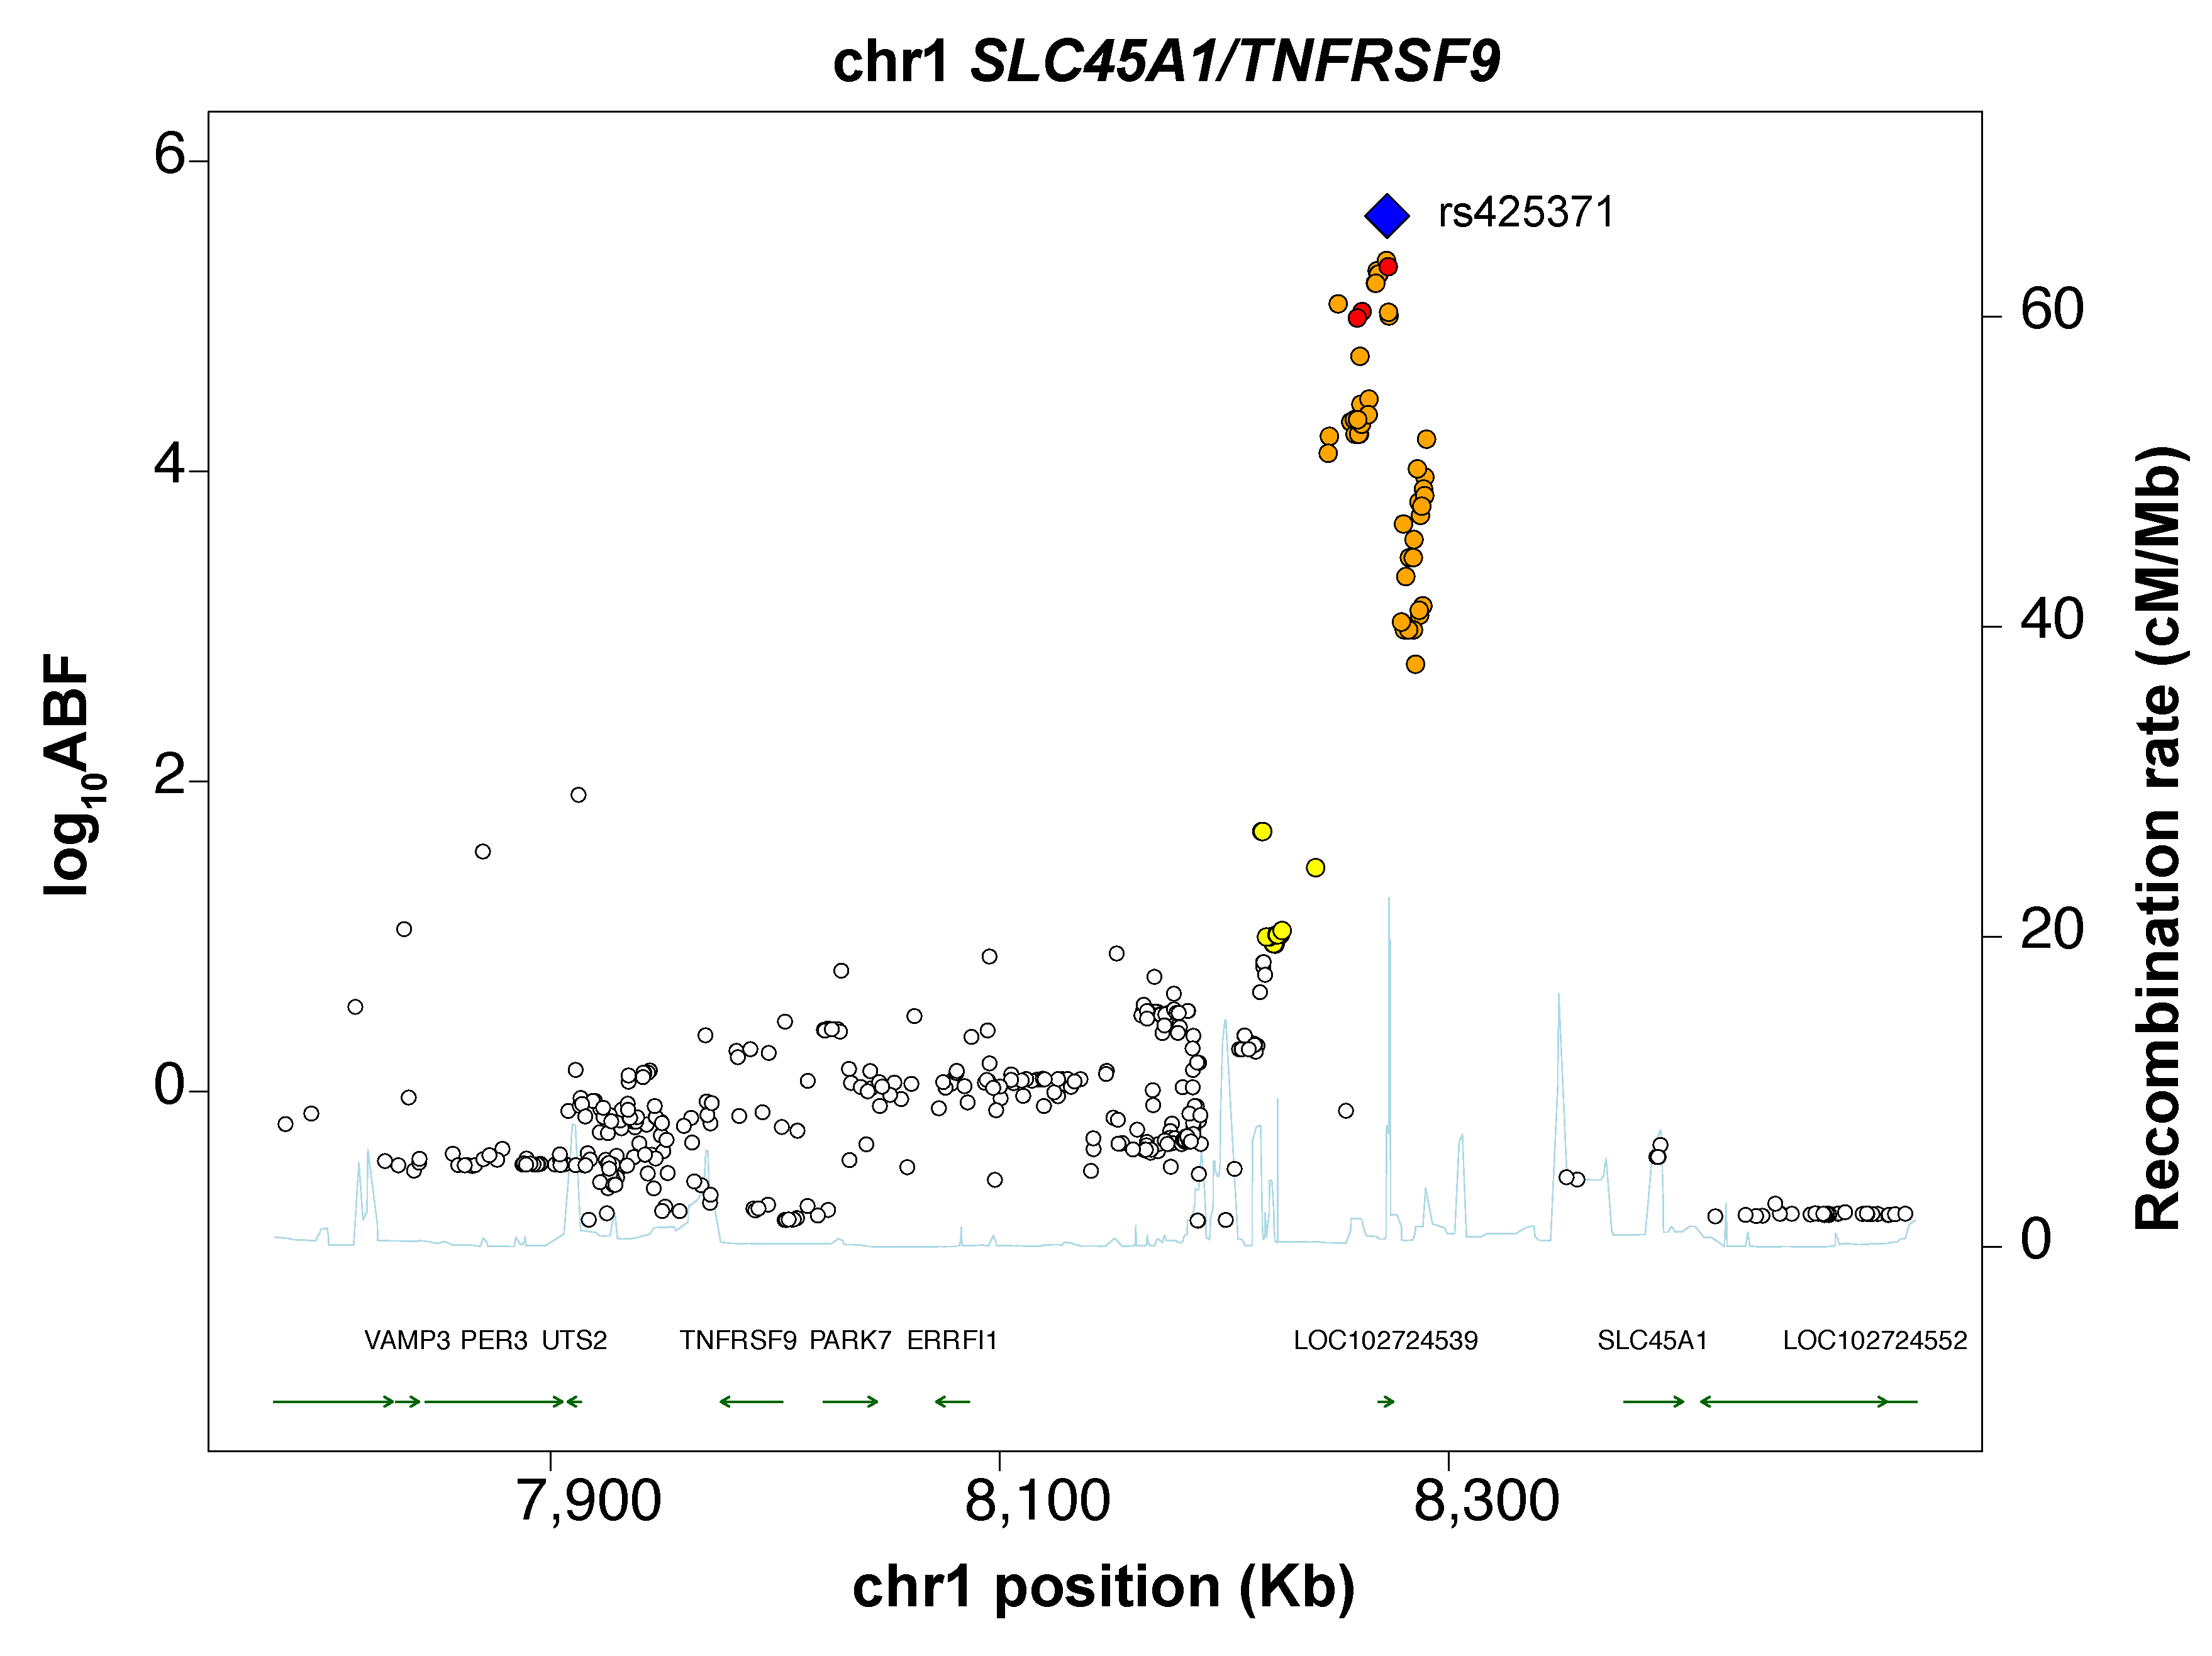
\includegraphics[width=0.65\textwidth]{./Results2/pdfs/PS_FM_Immunochip_TNFSRF9_association_plot}
\caption[Association plot for the fine-mapping using summary statistics from the psoriasis GAPC cohort Immunochip GWAS results of the \textit{SLC45A1/TNFRSF9} locus.]{\textbf{Association plot for the fine-mapping using summary statistics from the psoriasis GAPC cohort Immunochip GWAS results of the \textit{SLC45A1/TNFRSF9} locus.} For each of the SNPs (dot) the location (x-axis) and the log$_{10}$ABF (left y-axis) from the fine-mapping association analysis are shown. The colour of each dot indicated the LD relationship (r$^2$) with the lead SNPs (blue diamond), being white=low LD (r$^{2}<$0.2), yellow=weak LD (r$^{2}<$0.5), orange=moderate LD (r$^{2}<$0.8) and red=high LD (r$^{2}$$\geq$0.8). The recombination rates in this window of the genome is indicated in the right y-axis (light blue line).}
\label{figure:TNFRSF9_fine_mapping_association_plot}
\end{figure}




Amongst the four SNPs overlapping CD14$^+$ monocyte-specific ATAC peaks was the fine-mapping lead SNP rs425371, located at an intergenic region, 269.3Kb downstream the \textit{TNFRSF9} gene (Figure \ref{figure:ATAC_PS_CTL_TNFSF9_FM} top panel). The other three SNPs overlapping CD14$^+$ monocytes accessible chromatin were rs11121131, rs12745477 and rs417065 (Figure \ref{figure:ATAC_PS_CTL_TNFSF9_FM} top panel). Notably, the two ATAC peaks harbouring the four fine-mapped SNPs showed variable chromatin accessibility across individuals (Figure \ref{figure:ATAC_PS_CTL_TNFSF9_FM} bottom panel), enrichment for H3K4me1 CD14$^+$ monocytes Roadmap Epigenomics Project data and a modest enrichment for in-house H3K27ac data in some of the samples (Figure \ref{figure:ATAC_PS_CTL_TNFSF9_FM} bottom panel). This was consistent with enhancer designation in these two regions in the chromatin segmentation map for CD14$^+$ monocytes. No accessible chromatin was found at the location of the four fine-mapped SNPs in CD4$^+$, CD8$^+$ and CD19$^+$ cells, in line with the classification of these two regions as heterochromatin or repressed chromatin by the chromatin segmentation maps in the corresponding cell types. Furthermore, rs11121131, rs12745477 and rs417065 also overlapped with TF binding sites identified by ENCODE ChIP-seq data in a number of cell types and rs11121131 was nearby a CpG island (Figure \ref{figure:ATAC_PS_CTL_TNFSF9_FM} bottom panel), altogether reinforcing a putative role of these two regions in regulating gene expression. Integration with eQTL datasets revealed that rs12745477 and rs42537 had a modest effect in regulating \textit{PARK7} expression levels in CD14$^+$ monocytes treated with LPS for 24h (FDR=0.01) or in whole blood (FDR=0.04), respectively \parencite{Fairfax2012,Westra2013}. Promoter capture Hi-C data showed physical interaction between a bait containing rs12745477 and the \textit{ERRFI1} gene \parencite{Javierre2016}. Nevertheless, my data did not find differential expression for \textit{TNFRSF9}, \textit{SLC45A}, \textit{PARK7}, \textit{ERRFI1} or any of the other proximal genes between psoriasis patients and healthy controls in CD14$^+$ monocytes.


\begin{figure}[htbp]
\centering
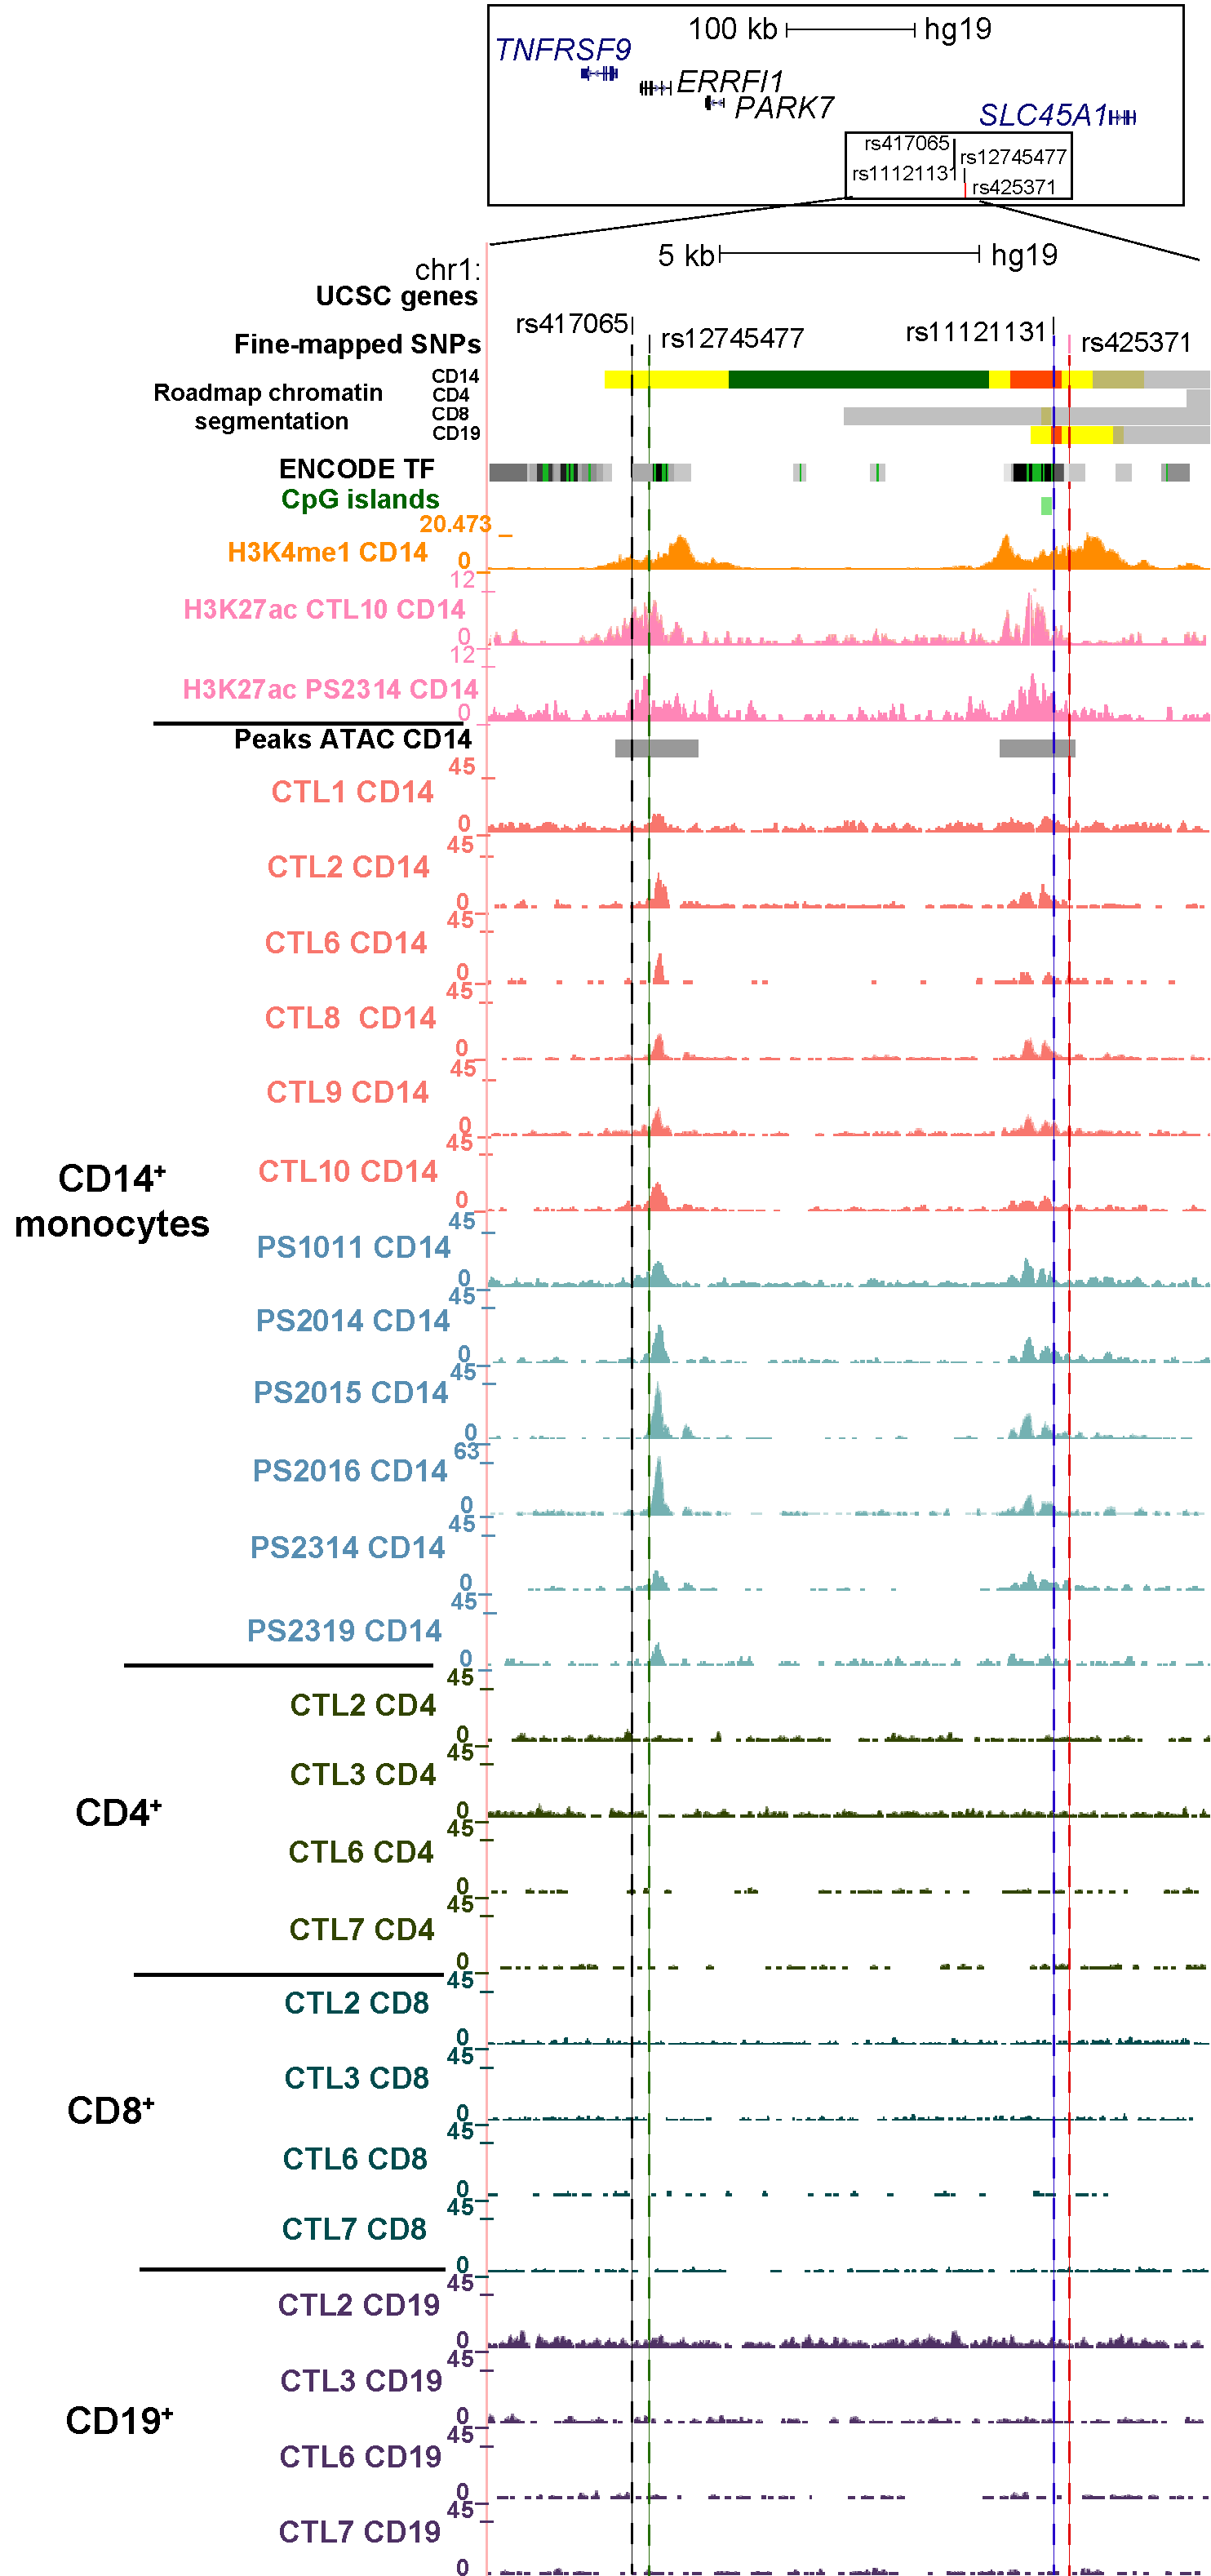
\includegraphics[width=0.55\textwidth]{./Results2/pdfs/UCSC_TNFRSF9_credible_set_track}
\caption[Epigenetic landscape at the location of the SNPs in the four SNPs in the 90\% credible set for the \textit{SLC45A1/TNFRSF9} psoriasis GWAS locus.]{\textbf{Epigenetic landscape at the location of the SNPs in the four SNPs in the 90\% credible set for the \textit{SLC45A1/TNFRSF9} psoriasis GWAS locus.} The top panel illustrates the genomic location of the four SNPs in the \textit{SLC45A1/TNFRSF9} fine-mapping 90\% credible set overlapping ATAC accessible regions in CD14$^+$ monocytes and their distance to the nearest genes. The bottom panel represents the UCSC Genome Browser view illustrating normalised ATAC read density and H3K27ac fold-enrichment as well as publicly available epigenetic datasets (chromatin segmentation map, H3K4me1, ENCODE TF ChIP-seq and CpG islands) (y-axis) at the location of the four SNPs (rs425371, rs11121131, rs12745477 and rs417065) (x-axis) from the credible set. Only representative ATAC tracks from control samples are shown for CD4$^+$, CD8$^+$ and CD19$^+$ cells to illustrate the absence of accessible chromatin at the location of the four SNPs.}
\label{figure:ATAC_PS_CTL_TNFSF9_FM}
\end{figure}





\subsection{Allele-specific differences in chromatin accessibility at the GWAS locus 2p15}
The chr2p15 psoriasis risk locus (lead SNP rs10865331, OR=1.12) is another of the psoriasis GWAS associations identified by the Immunochip study from Tsoi \textit{et al.} 2012 that is located in a large intergenic region. This locus is also shared with other chronic inflammatory diseases including AS and CD \parencite{Cortes2013,Jostins2012}. The fine-mapping using summary statistics from the psoriasis GAPC Immunochip performed here identified a signal with the lead SNP (rs9309343) showing log$_{10}$ABF=4.3; however it was not in LD with the psoriasis GWAS lead SNP from Tsoi \textit{et al.} 2012. Fine-mapping analysis on the AS UK Immunochip performed by Dr Anna Sanniti refined the 95\% credible set to three SNPs (rs4672505, rs6759298 and rs6759003), of which rs4672505 (risk allele rs4672505\_A) demonstrated the greatest PP (0.4). Notably, rs4672505 was also identified as the lead SNP for an association signal in Ellinghaus and colleagues multi-disease meta-analysis shared by psoriasis, AS and CD \parencite{Ellinghaus2016}.

rs4672505 overlaps a CD8$^+$ T cell-specific ATAC peak, not present in CD14$^+$ monocytes, CD4$^+$ and CD19$^+$ cells (Figure \ref{figure:ATAC_PS_CTL_chr2p15_rs4672505}A), that was not differentially accessible between patients and controls but did show marked variability across individuals (Figure \ref{figure:ATAC_PS_CTL_chr2p15_rs4672505}B), with some individuals (PS2314 and CTL1) demonstrating no ATAC signal at this location. 

Integration with publicly available ENCODE and Roadmap Epigenomics Project DHS data confirmed accessible chromatin at this site in Th-1, Th-2 and Th-17 cells and CD8$^+$ T cells, respectively (Figure \ref{figure:ATAC_PS_CTL_chr2p15_rs4672505}A). Variability across individuals was also observed for H3K27ac enrichment as per ChIPm data generated in cohort 1B (Figure \ref{figure:ATAC_PS_CTL_chr2p15_rs4672505}B). ENCODE ChIP-seq data from GM12878 showed binding at this location of RUNX3, a psoriasis and AS GWAS associated gene involved in CD8$^+$ cell differentiation \parencite{Wong2011}. In addition, \textit{in silico} TF binding sites prediction using PROMO \parencite{Messeguer2002} and ENCODE genomic DNase-I footprint in GM128778 predicted STAT1 binding at rs4672505. Altogether, integration of fine-mapping, ATAC and publicly available epigenetic data indicated that rs4672505 was the most likely causal functional variant accounting for the association of the 2p15 locus with psoriasis risk.


\begin{figure}[htbp]
\centering
\begin{subfigure}[b]{0.5\textwidth}
\centering
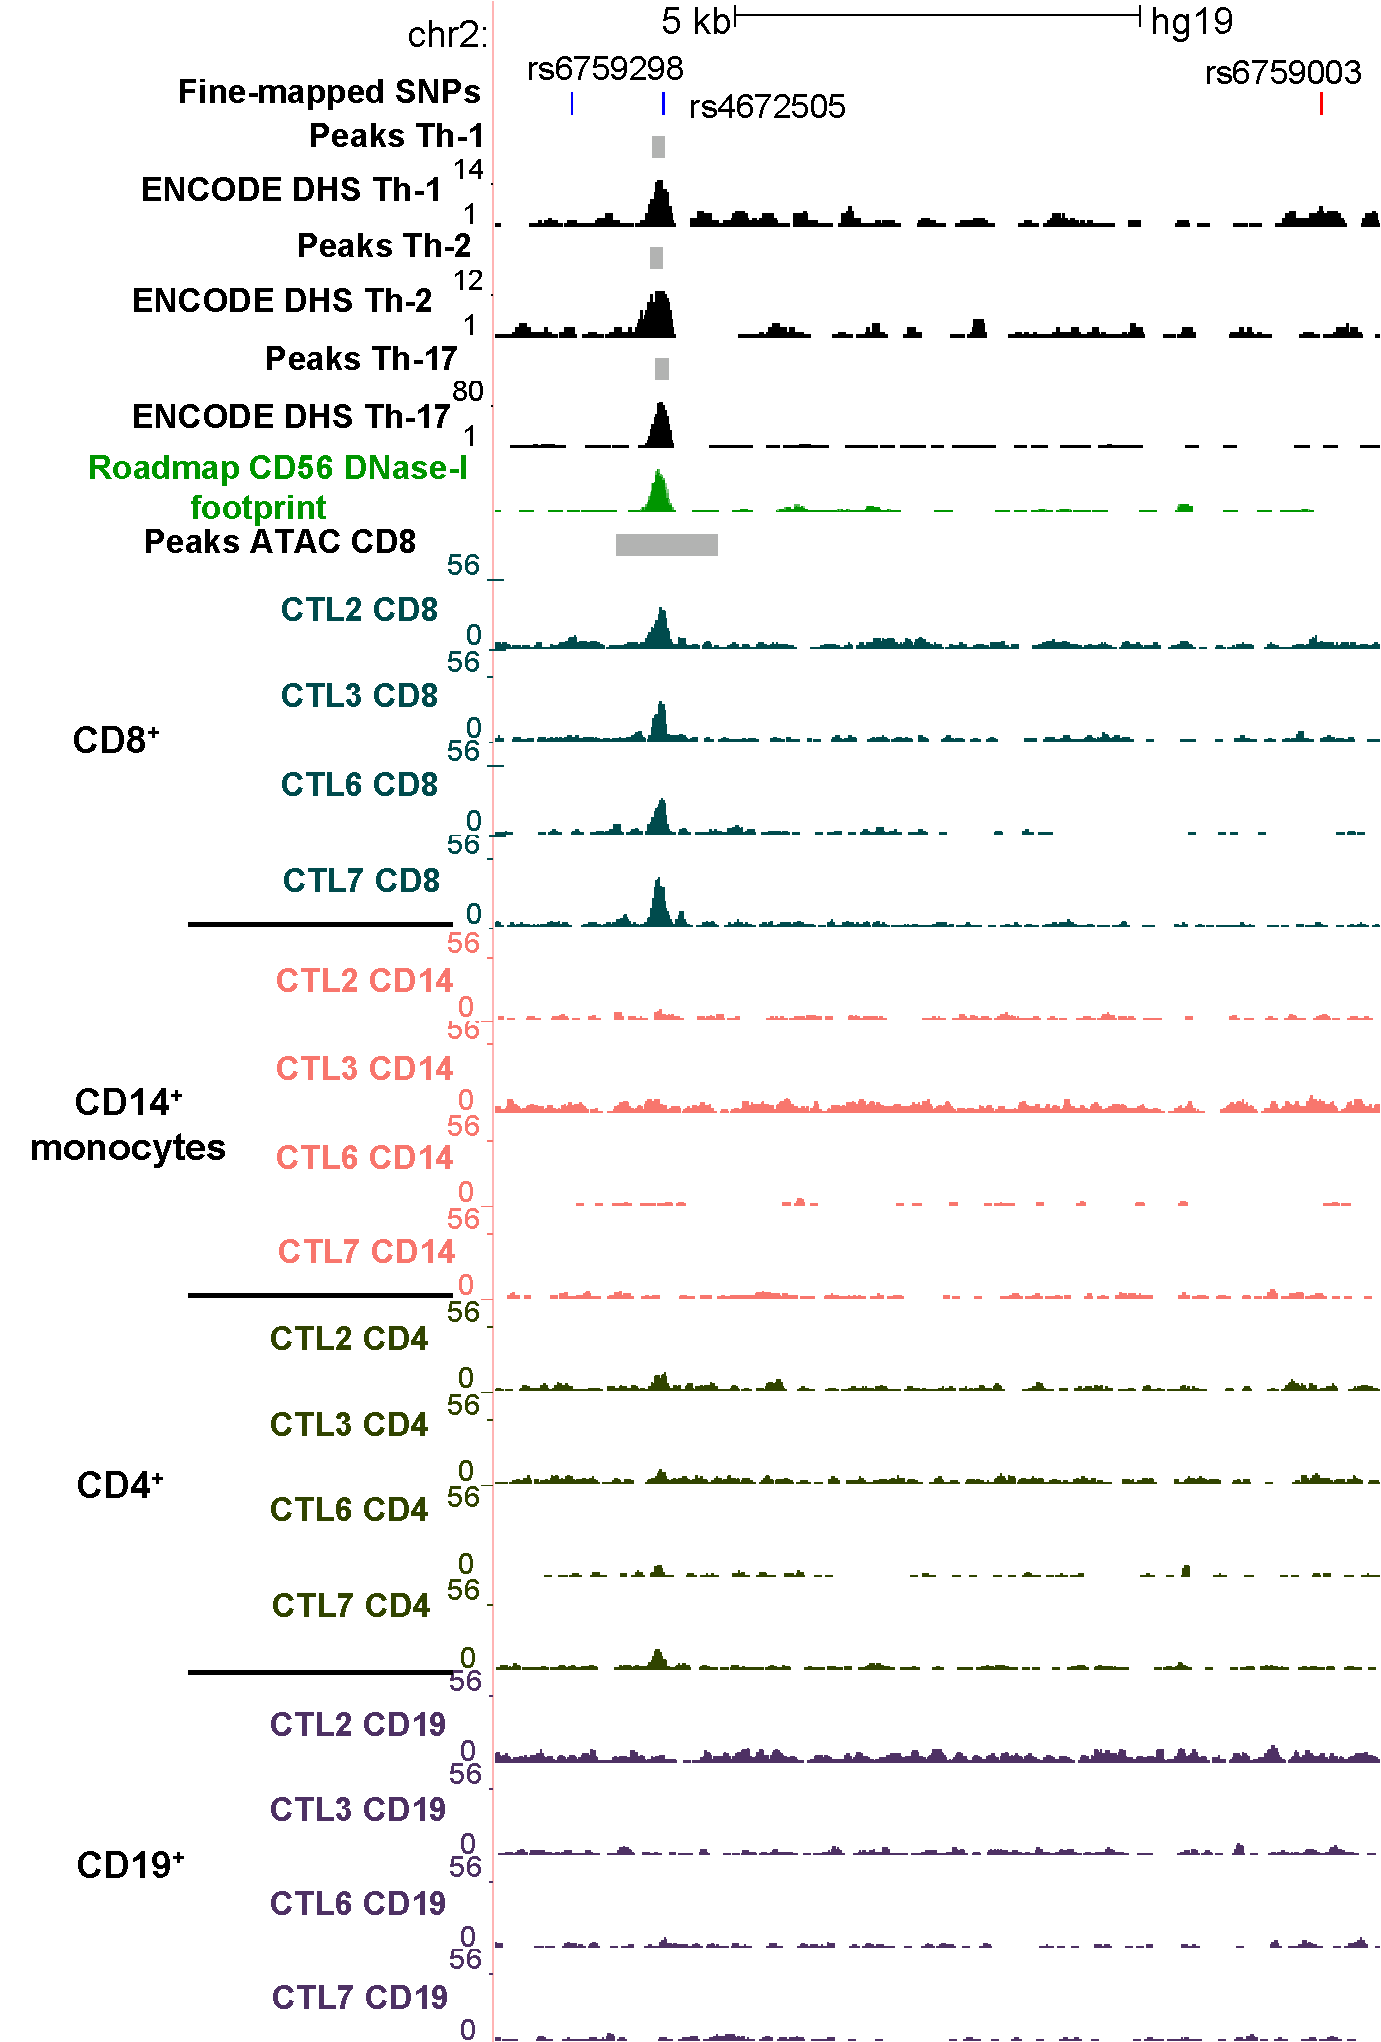
\includegraphics[width=\textwidth]{./Results2/pdfs/chr2p15_rs4672505_FM_all_cell_types_track_all_marks}
\caption{\textbf{}}
% The percentage sign indicated that the other subfig goes side by side
\end{subfigure}%
\begin{subfigure}[b]{0.45\textwidth}
\centering
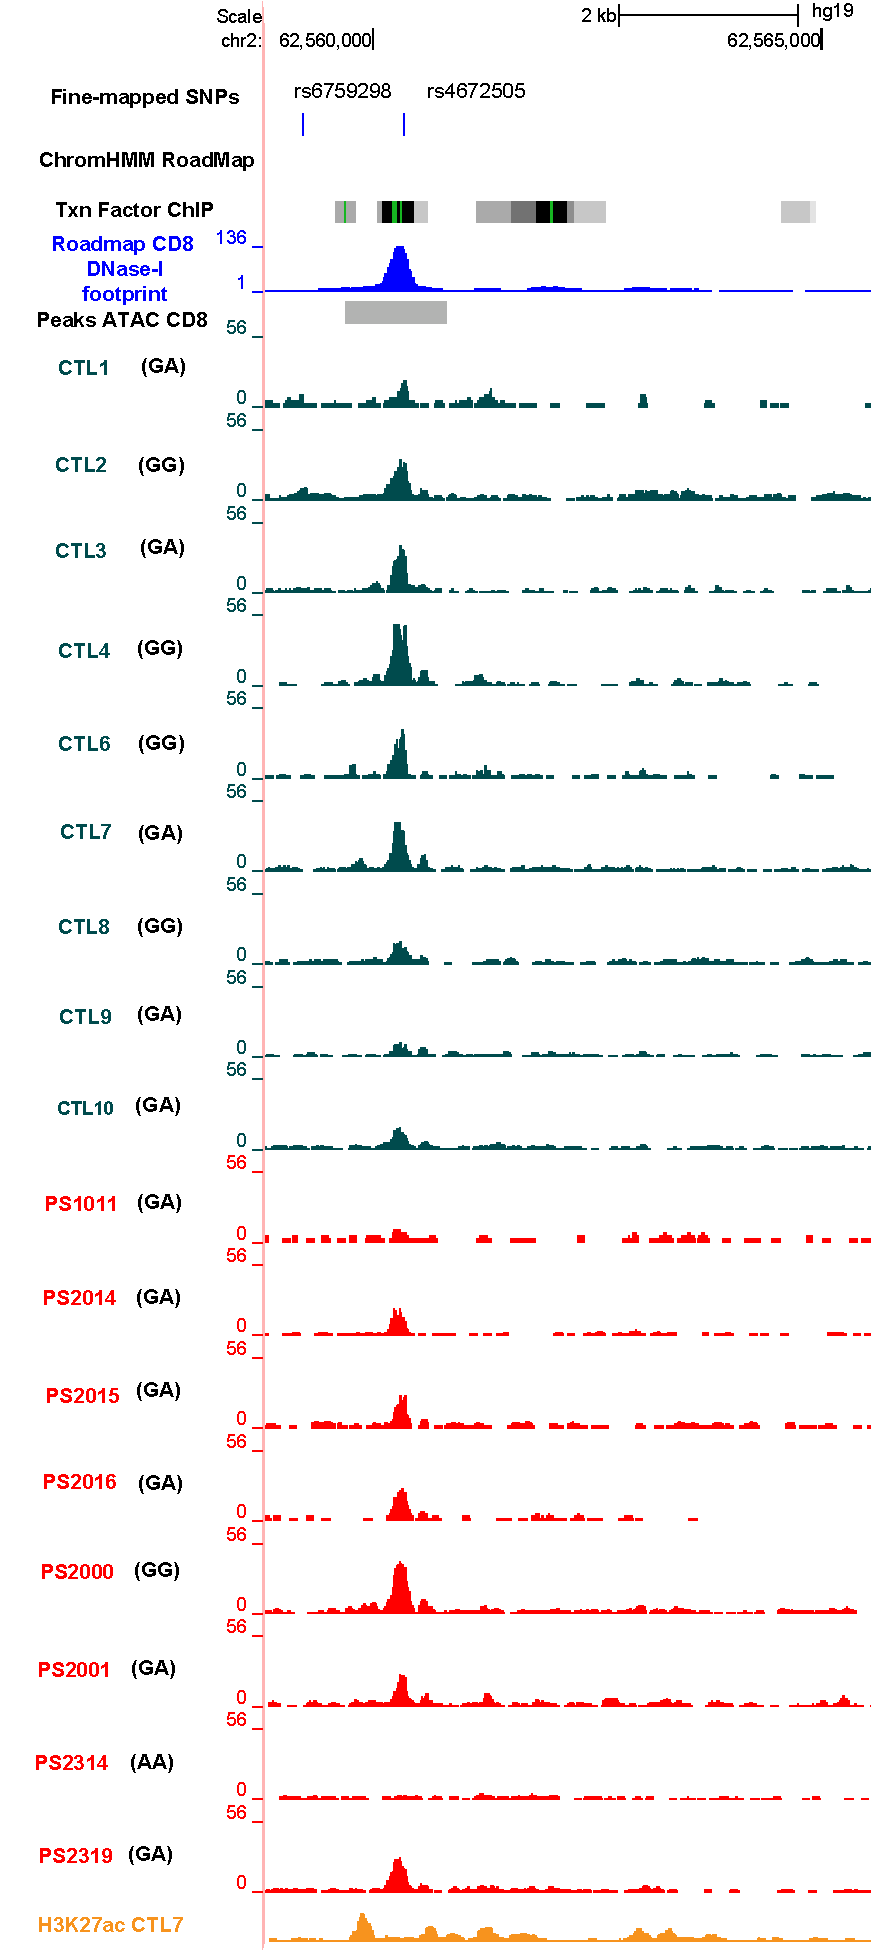
\includegraphics[width=\textwidth]{./Results2/pdfs/chr2p15_rs4672505_FM_CD8_track_all_marks}
\caption{\textbf{}}
\end{subfigure}
\caption[Epigenetic landscape at the location of the 95\% credible set of AS fine-mapped SNPs for the chr2p15.]{\textbf{Epigenetic landscape at the location of the 95\% credible set of AS fine-mapped SNPs for the chr2p15.} (A) UCSC Genome Browser view illustrating normalised read density for in-house ATAC and a number of other publicly available epigenetic data (DHS, DNAse-I footprint, chromatin segmentation map) (y-axis) snapping the three SNPs (rs6759298, rs4672505 and rs6759003) (x-axis) from the 95\% credible set obtained in the fine-mapping analysis of the chr2p15 GWAS association in AS. Representative ATAC data from the same four controls in the cohort and the four cell types included in this study are shown. (B) UCSC Genome Browser view illustrating the normalised read density for CD8$^+$ ATAC (x-axis) generated in psoriasis patients and healthy controls, in-house H3K27ac ChIPm, ENCODE TF ChIP-seq and DNase-I fooprint (y-axis) at the location of the SNP rs4672505 (y-axis). For each of the patients and controls of the cohort the Sanger sequencing genotype of rs4672505 is included.}
\label{figure:ATAC_PS_CTL_chr2p15_rs4672505}
\end{figure} 




% Not sure where to include the methyl QTLs

%\subsubsection{Allele-dependent chromatin accessibility and allelic imbalance using ATAC reads at rs4672505}
The genotype at rs4672505 of each individual was determined using Sanger sequencing. Amongst the eighteen samples (ten controls and eight psoriasis patients), one (PS2314) was homozygous for the risk allele (A, MAF=0.43), 11 were heterozygous and 6 were homozygous for the protective allele (G) (Figure \ref{figure:ATAC_PS_CTL_chr2p15_rs4672505}B). Interestingly, PS2314, the only homozygous individual for the risk allele, showed complete absence of the ATAC peak at rs4672505. To further investigate the role of rs4672505 genotype in the variability of chromatin accessibility across individuals, normalised read counts at the ATAC peak chr2:62,559,749-62,561,442 were used as a dependent variable in linear model analysis based on rs4672505 genotype, using batch as a covariate. 



\begin{figure}[htbp]
\centering
\begin{subfigure}{0.45\textwidth}
\centering
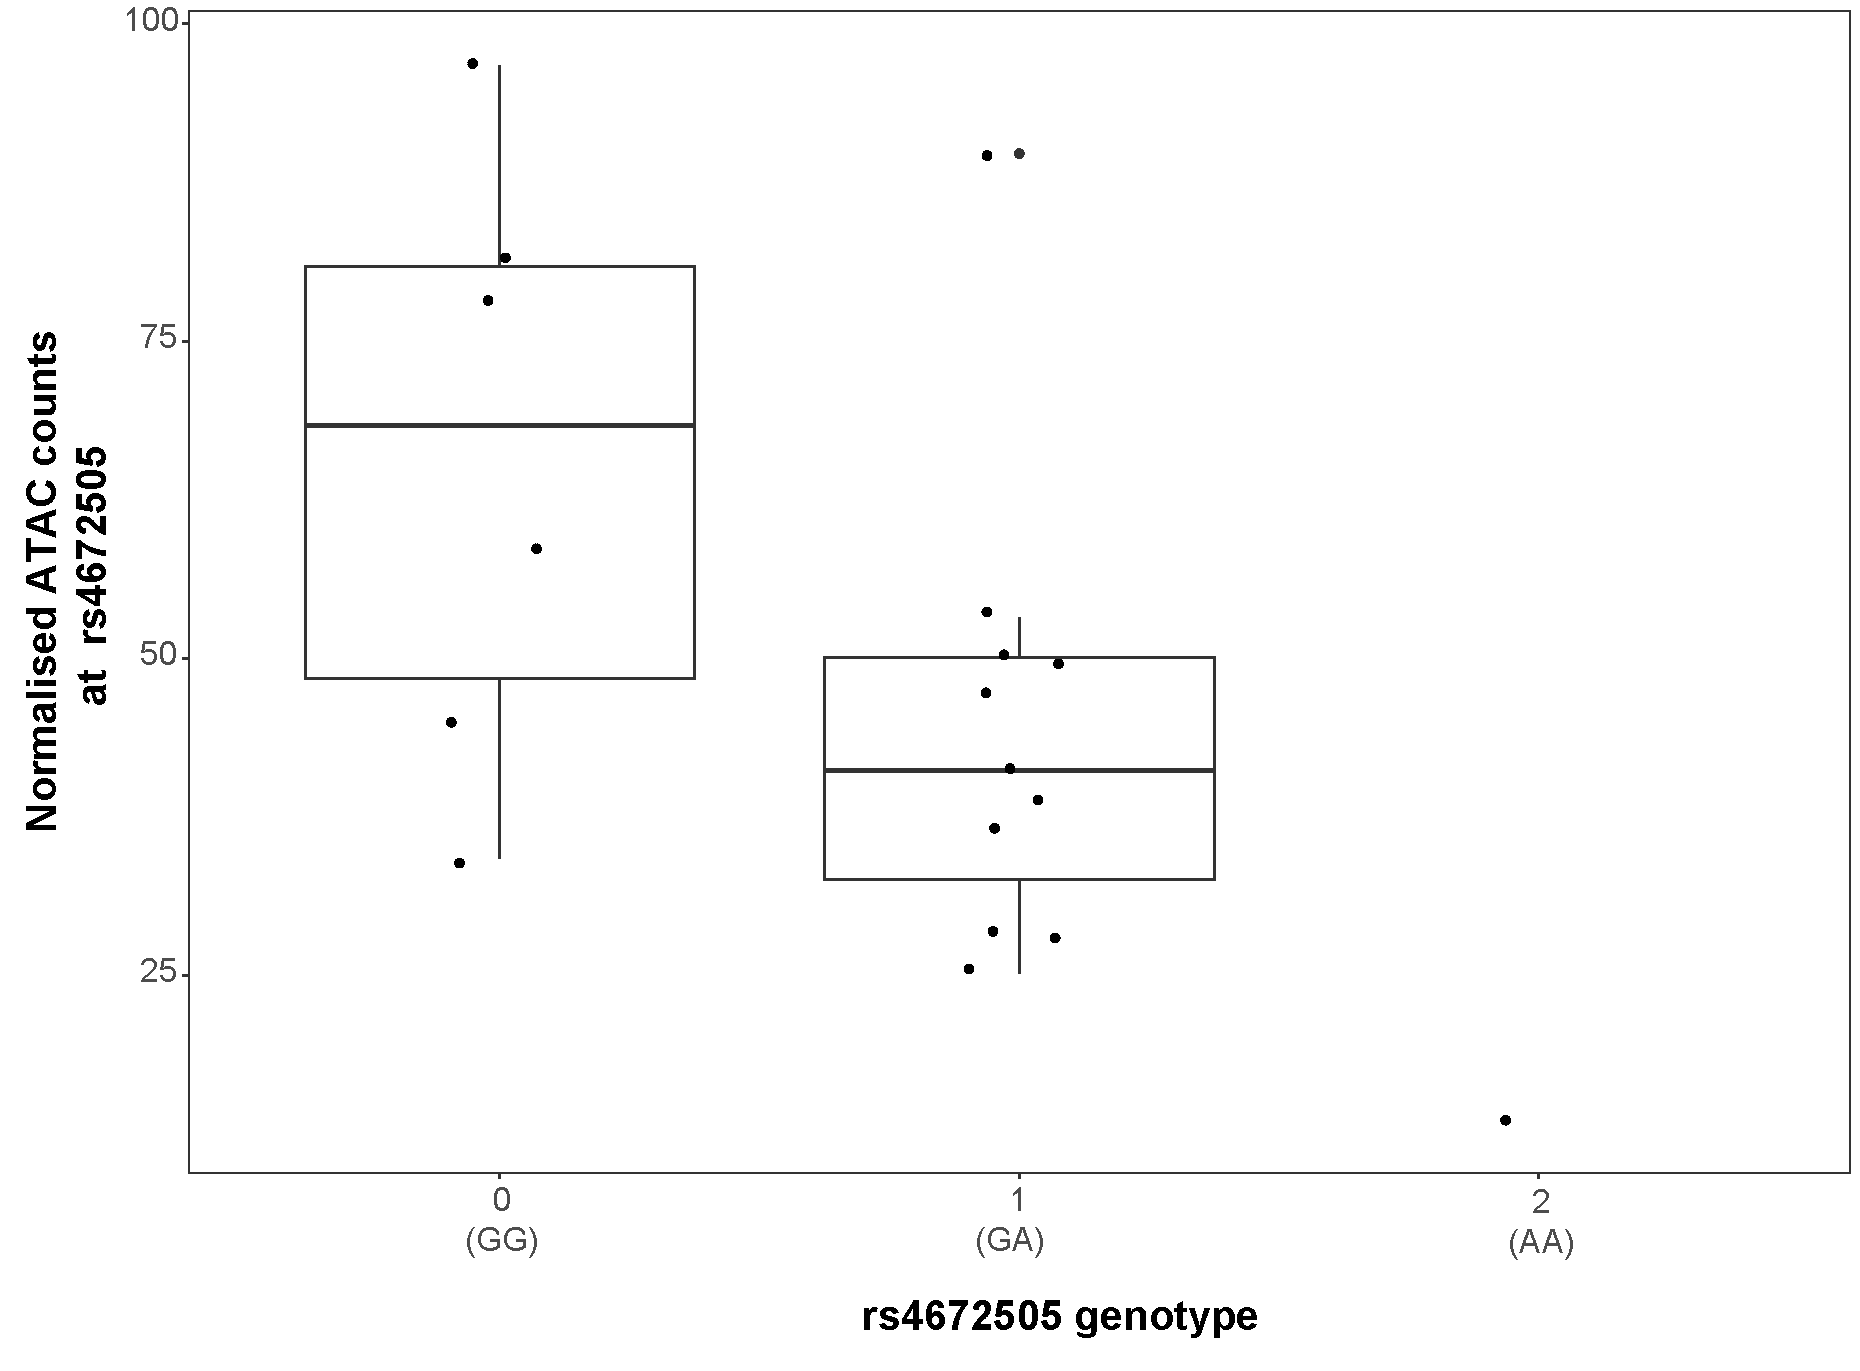
\includegraphics[width=\textwidth]{./Results2/pdfs/ATAC_caQTL_CD8_final}
\caption{\textbf{}}
% The percentage sign indicated that the other subfig goes side by side
\end{subfigure}%
\begin{subfigure}{0.45\textwidth}
\centering
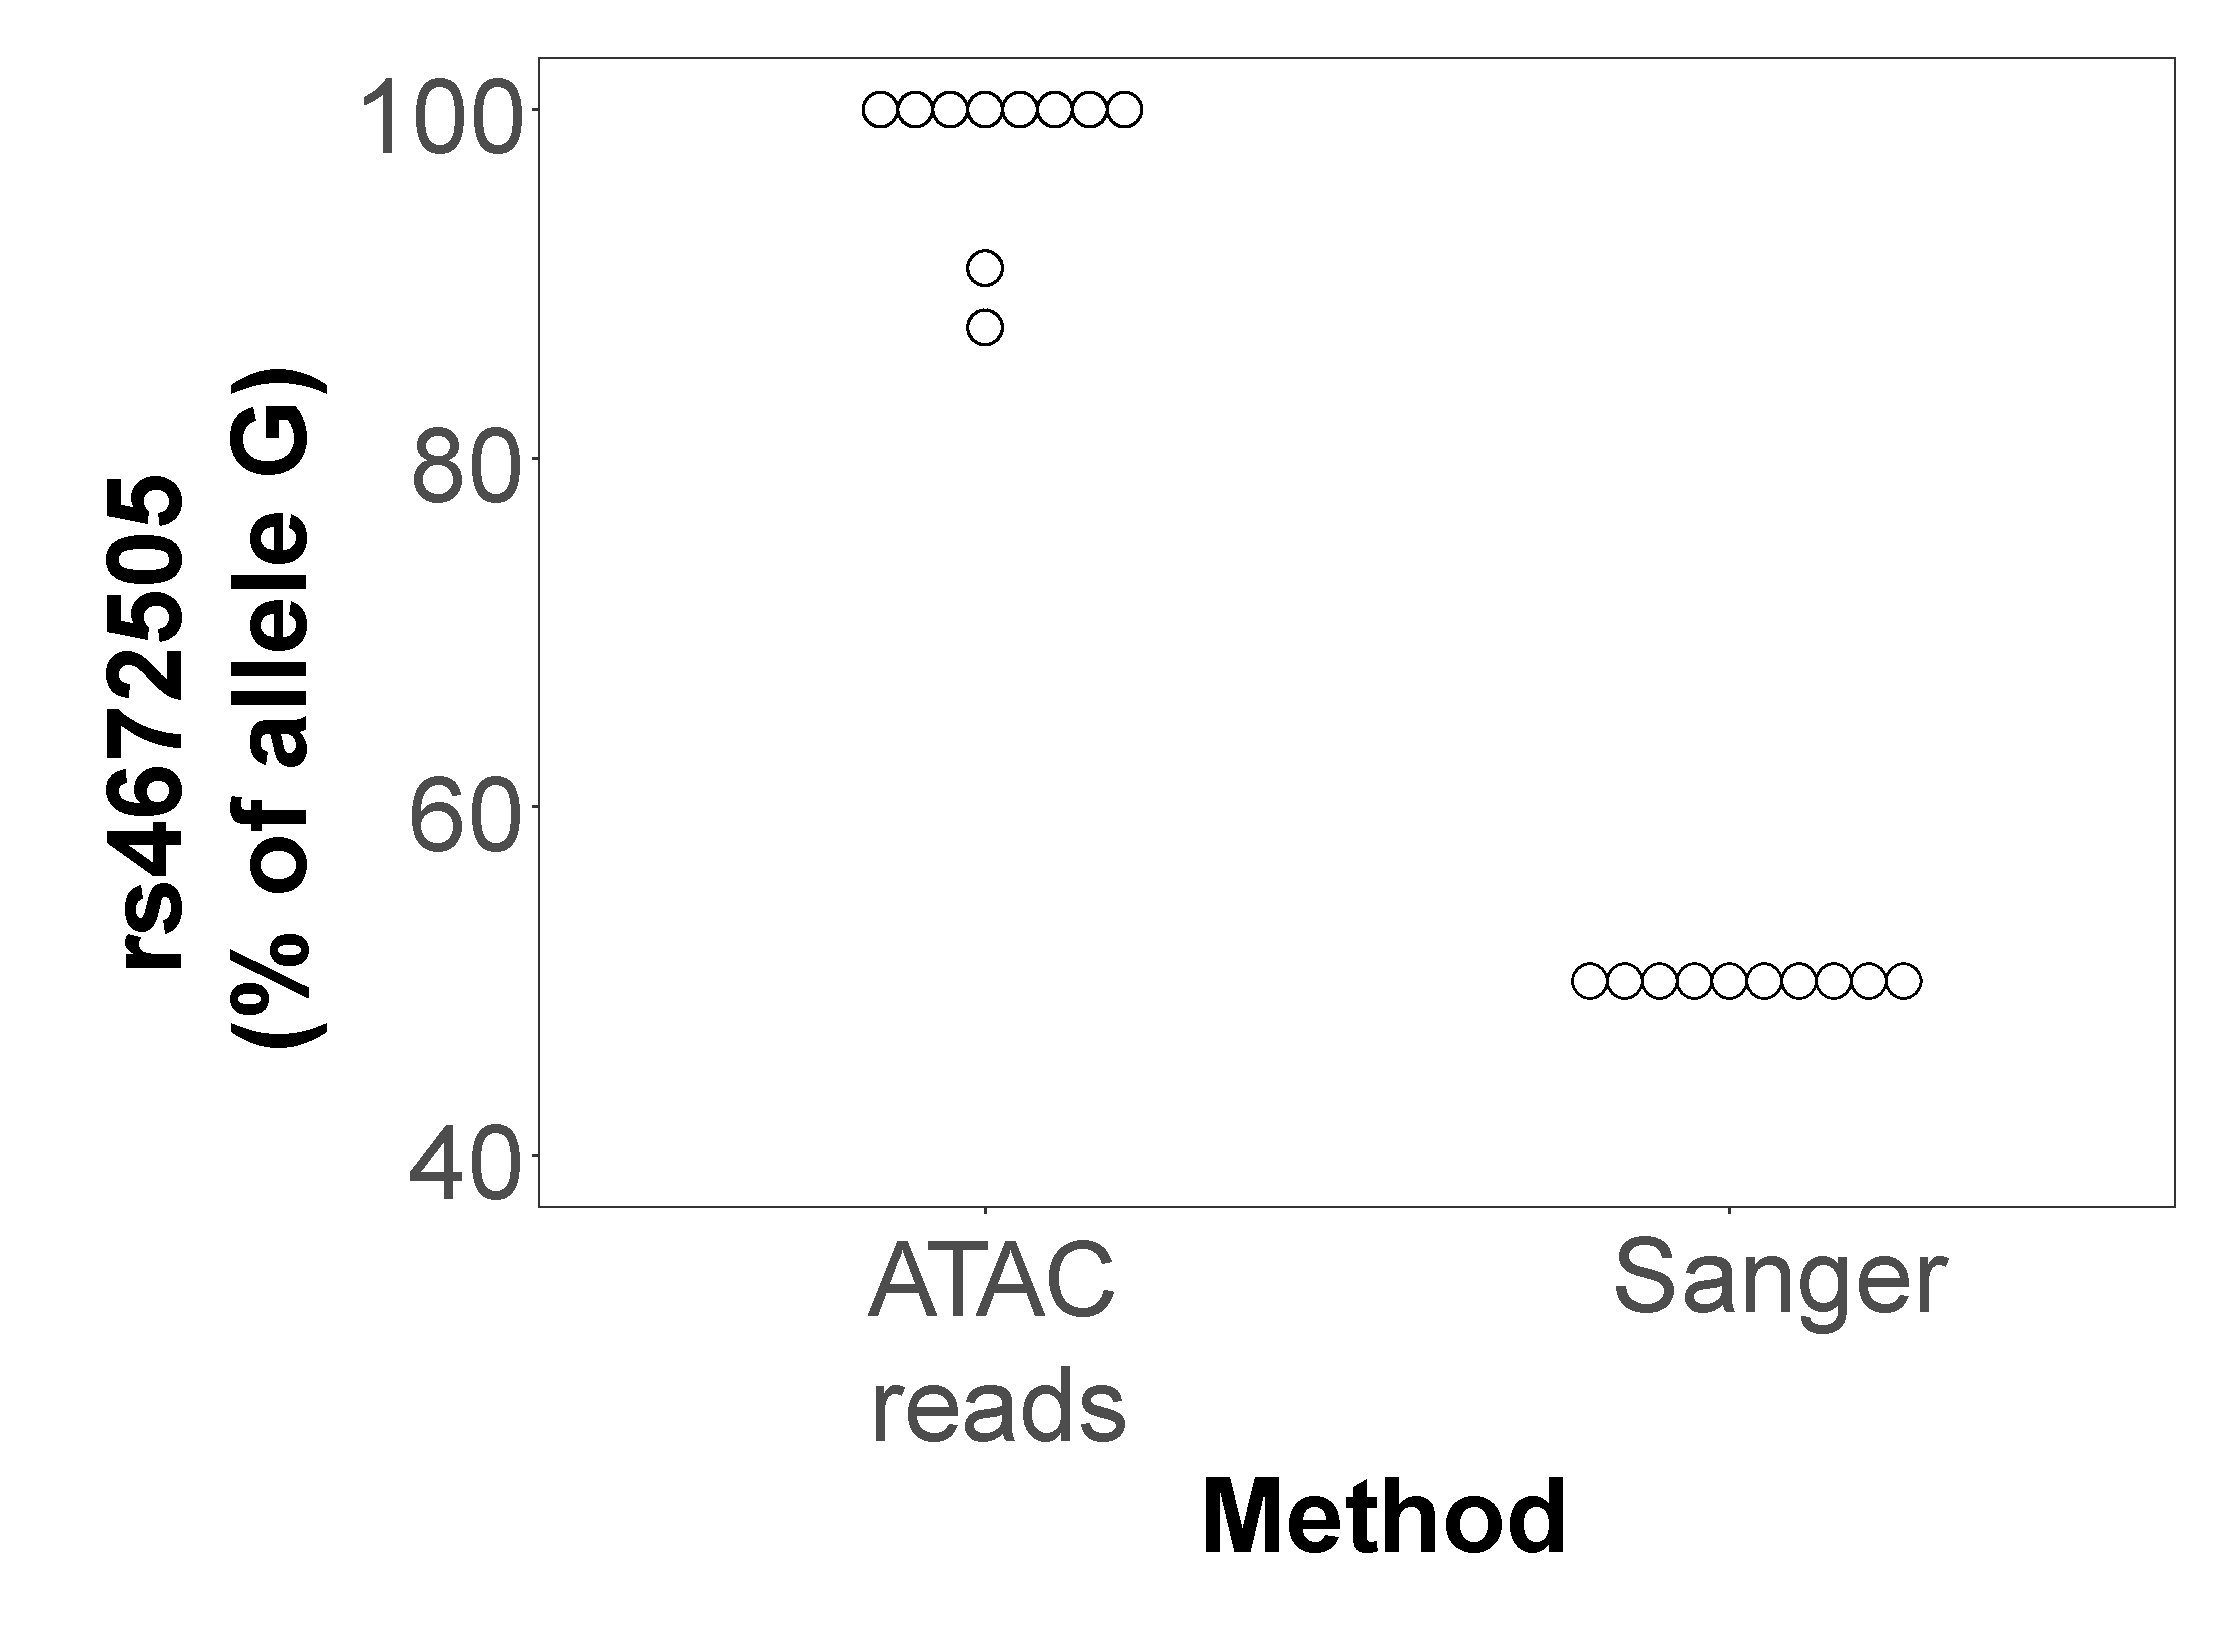
\includegraphics[width=\textwidth]{./Results2/pdfs/chr2p15_rs4672505_allelic_imbalance_CD8_final}
\caption{\textbf{}}
\end{subfigure}
\caption[rs4672505 genotype and chromatin accessibility at chr2:62,559,749-62,561,442 in CD8$^+$ cells.]{\textbf{rs4672505 genotype and chromatin accessibility at chr2:62,559,749-62,561,442 in CD8$^+$ cells.} (A) Boxplot illustrating the effect of the rs4672505 genotype on chromatin accessibility at the chr2:62,559,749-62,561,442 ATAC peak. Log$_2$ normalised ATAC read counts adjusted for batch effect (included as a covariate for the linear model) are plotted for each sample against the number of copies of the minor allele (GG=0, AG=1, AA=2). (B) Representation of the percentage of ATAC reads mapping to the major allele (G) at rs4672505 in comparison to the Sanger genotype results for the 11 heterozygous individuals.}
\label{figure:ATAC_PS_CTL_caQTL_and_allelic_imbalance}
\end{figure} 
 
Significant negative correlation (p-value=0.035) was found, suggesting allele-dependent chromatin accessibility (Figure \ref{figure:ATAC_PS_CTL_caQTL_and_allelic_imbalance}A). Furthermore, allelic imbalance of ATAC reads at rs4672505 position was investigated in individuals identified as heterozygous by Sanger sequencing, for which 50\% of the ATAC reads were expected to map to each of the alleles. This analysis demonstrated a larger percentage of ATAC reads (greater than the expected 50\%) preferentially tagging the protective allele G (Figure \ref{figure:ATAC_PS_CTL_caQTL_and_allelic_imbalance}B). This finding was not driven by mapping bias, since A was the reference allele in the hg19 build used in this analysis. Overall, these results showed evidence of greater chromatin accessibility in presence of the fine-mapped protective allele rs4672505(G) at the chr2p15 locus.
 

%\subsubsection{Potential regulatory role of rs4672505 in the expression of B3GNT2}
A major challenge with intergenic GWAS signals is the difficulty in determining the specific gene they may be modulating, for example through differential enhancer activity affecting gene expression. rs4672505 is located 140Kb downstream of \textit{B3GNT2} and 150Kb upstream of \textit{TMEM1}. Publicly available promoter capture Hi-C data from Javierre \textit{et al.} 2016 in CD8$^+$ revealed a significant physical interaction (CHiCAGO score=7.67) between the region containing rs4672505 and the promoter of \textit{B3GNT2} (Figure \ref{figure:RNA_chromatin_interaction_B3GNT2}A). This interaction was not found in any of the additional 16 human primary hematopoietic cell included in the study and no upstream interaction with \textit{TMEM1} promoter was identified. Investigation of the publicly available T cell eQTL dataset from Kasela \textit{et al.} and Raj \textit{et al.} did not show a significant eQTL for rs4672505 or SNPs in high LD (r$^2$$>$0.8) either in CD8$^+$ or CD4$^+$ \parencite{Raj2014,Kasela2017}. Similarly, no eQTL effect of rs4672505 was found in unstimulated or stimulated CD14$^+$ monocytes \parencite{Fairfax2014}. However, a whole blood eQTL study from Jansen and colleagues revealed a significant \textit{cis}-eQTL (FDR=1.34x10$^-5$) with moderate effect size ($\beta$=-0.16) for the minor allele \parencite{Jansen2017}. Differential gene expression analysis in circulating immune cells (previously presented) showed significant down-regulation (FDR$<$0.05) of \textit{B3GNT2} expression in psoriasis patients when compared to controls in CD8$^+$ cells (fold change=0.80) (Figure \ref{figure:RNA_chromatin_interaction_B3GNT2}B). 

Altogether, these data showed evidence of allele-specific chromatin accessibility at chr2p15 in CD8$^+$ T cells involving rs4672505, with chromatin conformation capture and gene expression data suggesting that this SNP may modulates expression of \textit{B3GNT2}, at a distance, and providing new insights into the possible mechanistic basis of the disease association seen in psoriasis, AS and CD for this locus.


\begin{figure}[htbp]
\centering
\begin{subfigure}{0.9\textwidth}
\centering
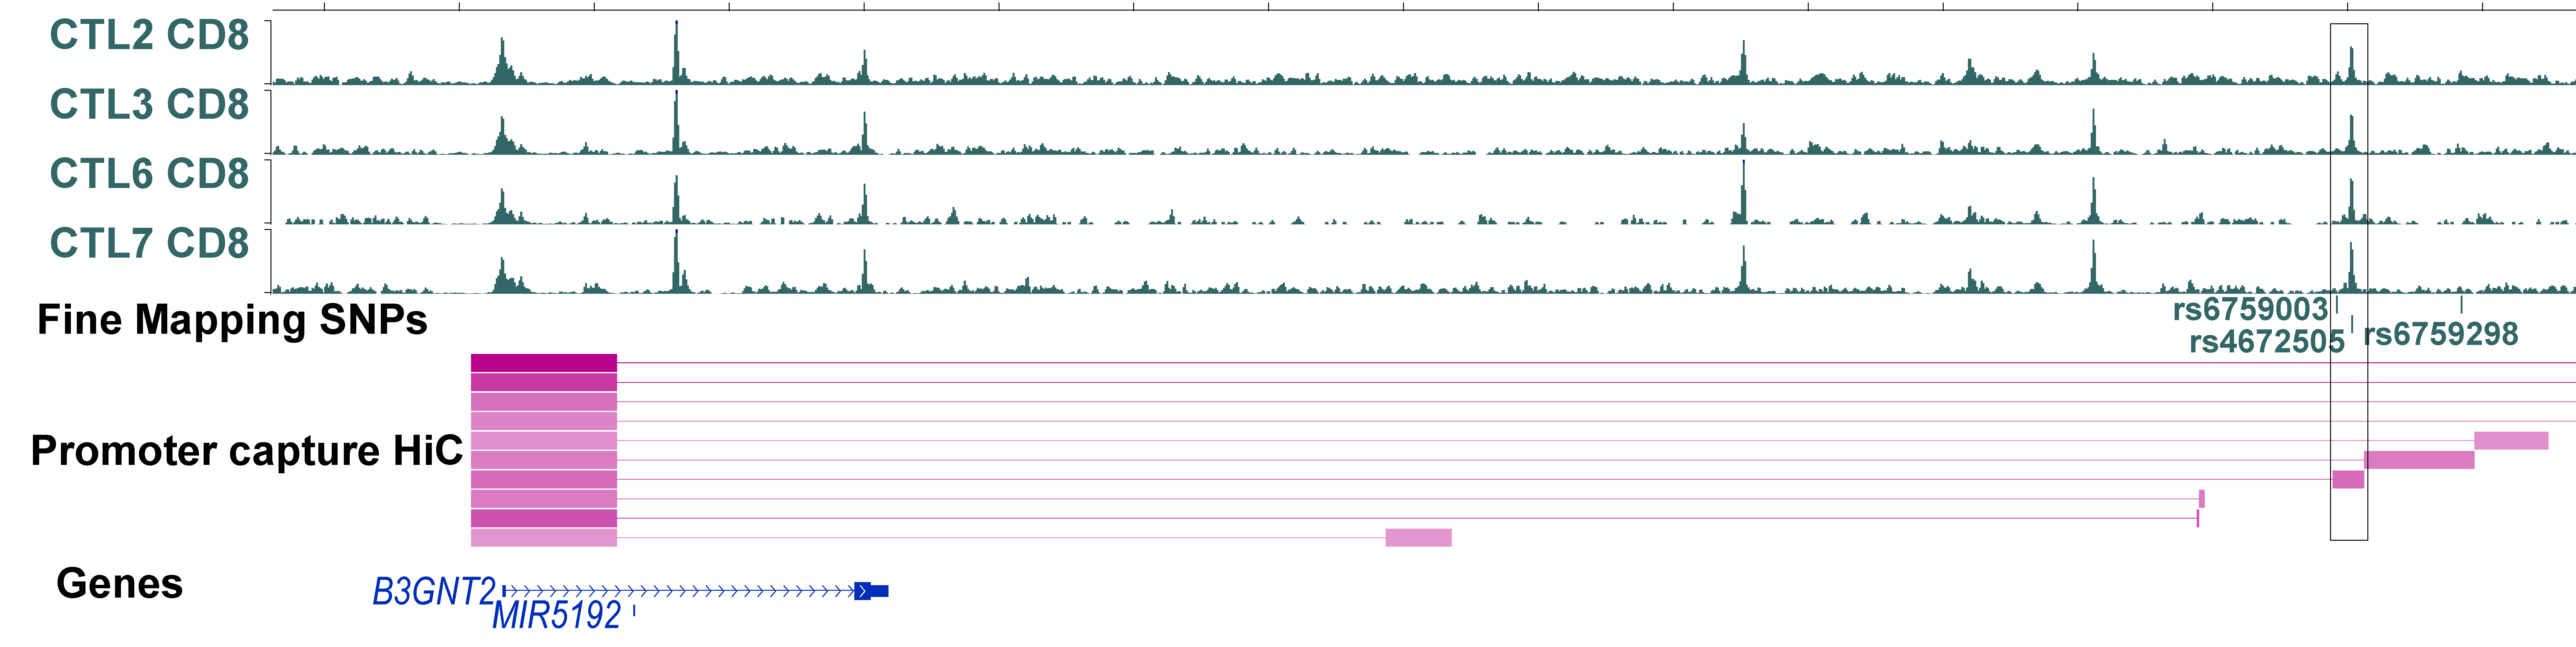
\includegraphics[width=\textwidth]{./Results2/pdfs/B3GNT2_HiC_WASHU_track}
\caption{\textbf{}}
% The percentage sign indicated that the other subfig goes side by side
\end{subfigure}
\begin{subfigure}{0.4\textwidth}
\centering
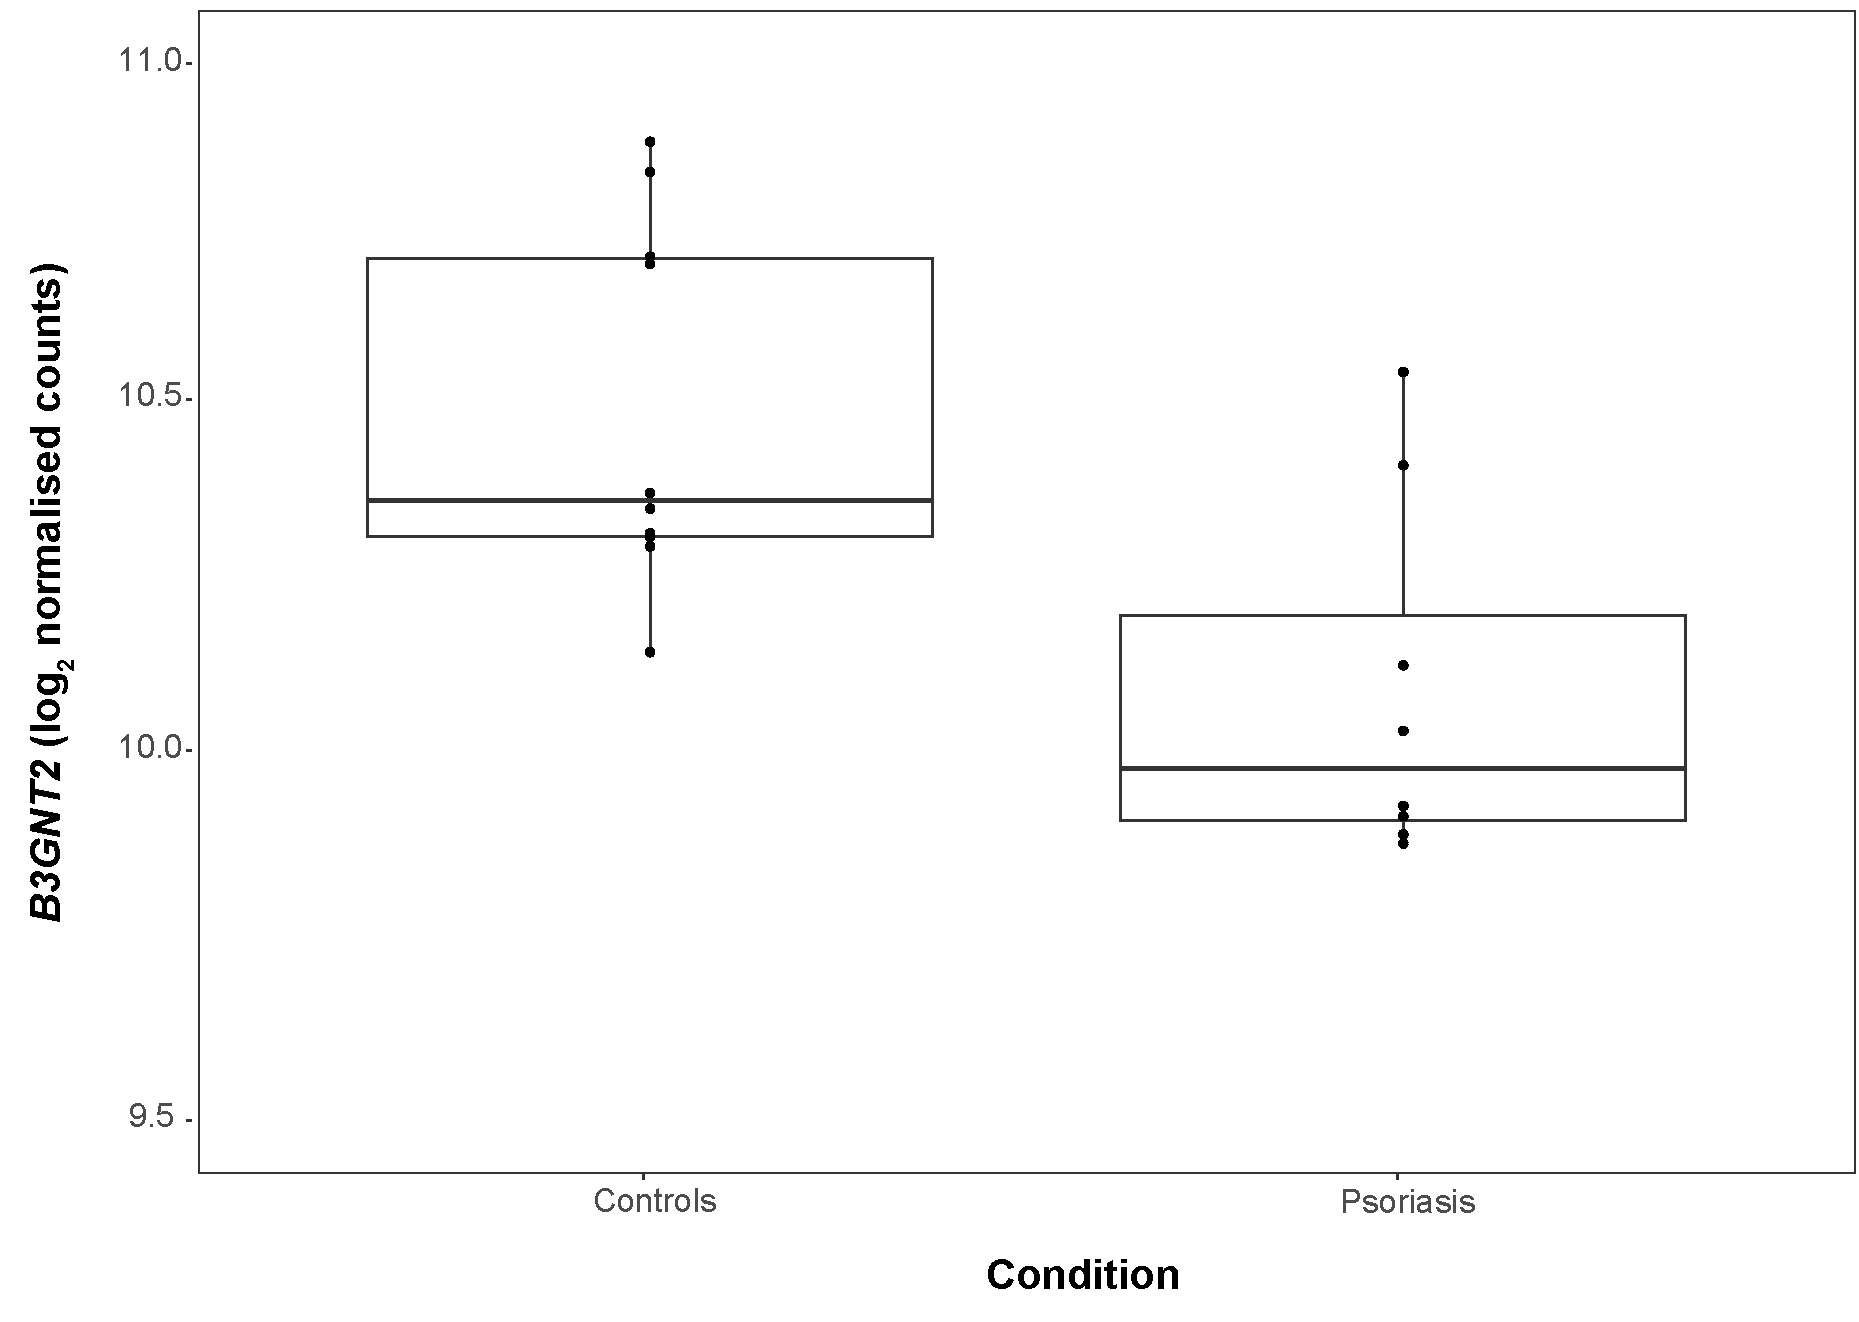
\includegraphics[width=\textwidth]{./Results2/pdfs/RNA_PS_CTL_B3GNT2_expression_CD8}
\caption{\textbf{}}
\end{subfigure}
\caption[Potential role of rs4672505 in regulating \textit{B3GNT2} gene expression.]{\textbf{Potential role of rs4672505 in regulating \textit{B3GNT2} gene expression.} (A) WASHU Genome Browser track showing normalised ATAC read density in four of the healthy controls CD8$^+$ cells at the location of the three SNPs in the 95\% credible set (AS fine-mapping analysis) and the promoter capture Hi-C data depicting the regions interacting with viewpoint at the \textit{B3GNT2} promoter. (B) Boxplot illustrating the \textit{B3GNT2} log$_2$ normalised RNA-seq counts adjusted for batch effect in psoriasis and healthy controls.}
\label{figure:RNA_chromatin_interaction_B3GNT2}
\end{figure} 






%\subsection{Maximising genetic commonalities across chronic inflammatory diseases: locus 2p15}
%The chr2p15 psoriasis risk locus (lead SNP rs10865331, OR=1.12) represents one of the GWAS associations located in an intergenic region was identified by the Immunochip study from Tsoi \textit{et al.},2012. This locus is shared with the chronic inflammatory diseases AS and CD. Interestingly, Reveille's AS GWAS study reported the same lead SNP as the psoriasis Immunochip \parencite{Reveille2010}. The later AS Immnochip study identified rs6759298 (OR=1.29) as the tag SNP for this region, which is in high LD (r$^2$=0.84) with rs10865331 \parencite{Cortes2012}. A recent GWAS meta-analysis combining data for five chronic inflammatory diseases also identified association for the chr2p15 locus, confirming the same association and direction to be shared by the three out of five phenotypes \parencite{Ellinghaus2016}. Therefore the AS and psoriasis associations are considered to be the same signal and likely to share the functional mechanism increasing the risk of a dysregulated inflammatory response.
%
%As previously presented, fine-mapping using summary statistics from the psoriasis GAPC Immunochip cohort failed to successfully fine-map this locus (log$_{10}$ABF<3). In contrast, genotype-based fine-mapping analysis performed in collaboration with Dr Anna Sanniti in the UK Immunochip AS data successfully identified an independent signal at chr2p15 (log$_{10}$ABF=18.43) tagged by the SNP rs4672505. The refinement of this association signal in AS yielded a 95\% credible set containing only three SNPs. Out of the three identified SNPs, rs4672505 accounted for 40\% of the association in chr2p15 locus whereas the additional two SNPs (rs6759298 and rs6759003) explained together 60\% of this association. Interestingly, the SNP rs4672505 was also the lead SNP for the chr2p15 signal identified in the multi-disease meta-analysis from Ellinghaus and colleagues, where the risk allele was found to be A, similar to the results in the AS GWAS association analysis performed for fine-mapping \parencite{Ellinghaus2016}.
%
%\subsubsection{Integration of ATAC and publicly available epigenetic data}
%rs4672505 overlaps an accessible ATAC region included in the CP\_CD8 and not present in CD14$^+$ monocytes, CD4$^+$ and CD19$^+$ cells (Figure \ref{figure:ATAC_PS_CTL_chr2p15_rs4672505}A). The CD8$^+$ accessible region harbouring rs4672505 was not a DAR between patients and controls and appeared to have variability across individuals unrelated to disease status (Figure \ref{figure:ATAC_PS_CTL_chr2p15_rs4672505}B). 
%
%
%\begin{figure}[htbp]
%\centering
%\begin{subfigure}[b]{0.5\textwidth}
%\centering
%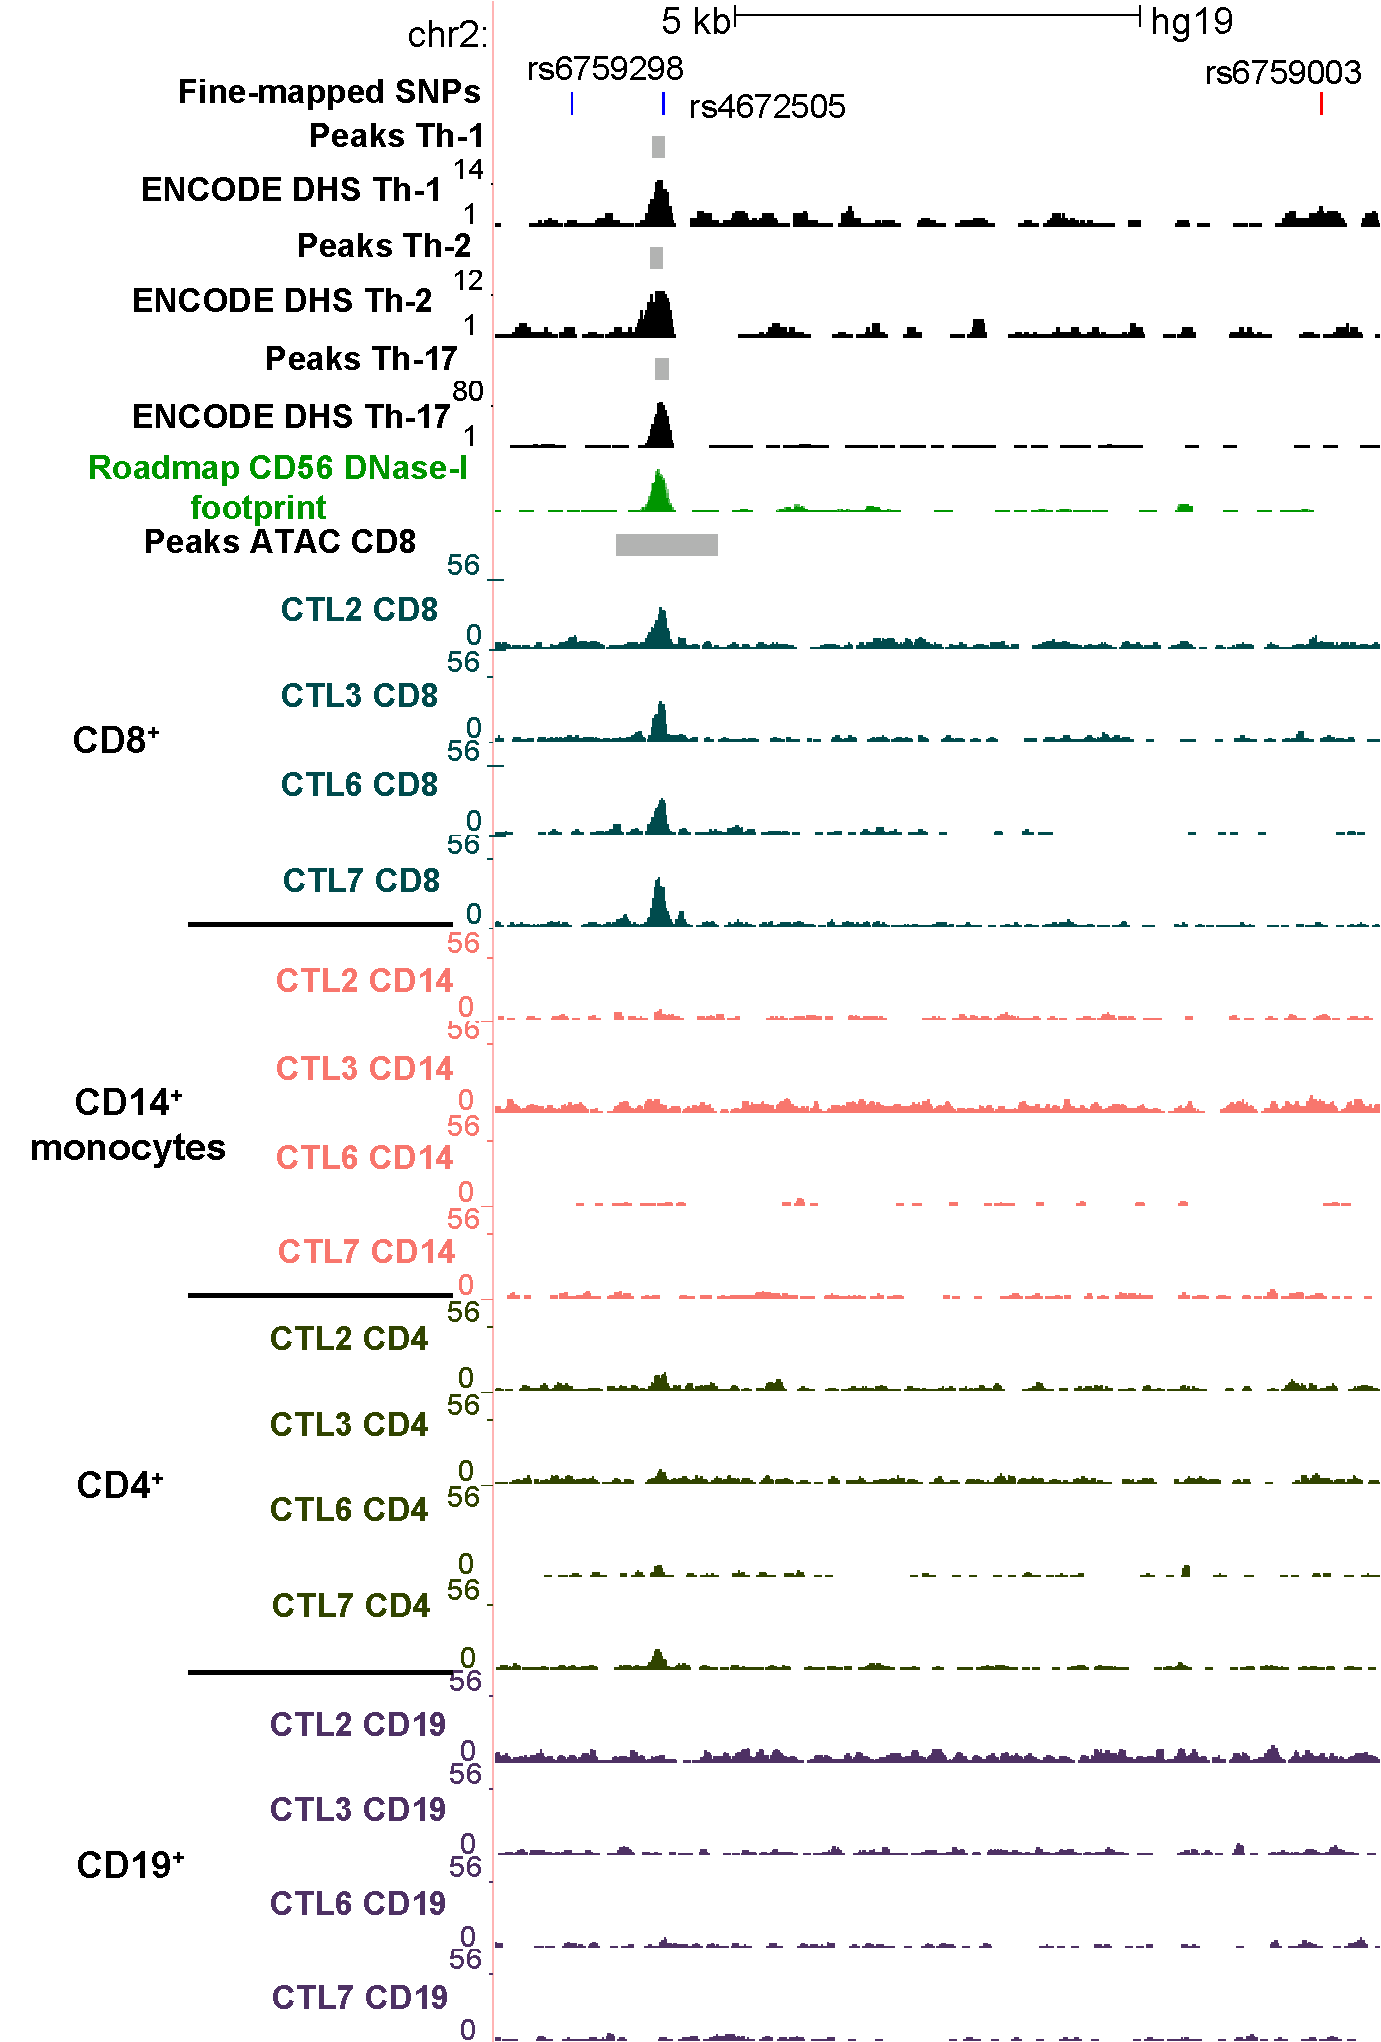
\includegraphics[width=\textwidth]{./Results2/pdfs/chr2p15_rs4672505_FM_all_cell_types_track_all_marks}
%\caption{\textbf{}}
%% The percentage sign indicated that the other subfig goes side by side
%\end{subfigure}%
%\begin{subfigure}[b]{0.45\textwidth}
%\centering
%\includegraphics[width=\textwidth]{./Results2/pdfs/chr2p15_rs4672505_FM_CD8_track_all_marks}
%\caption{\textbf{}}
%\end{subfigure}
%\caption[Epigenetic landscape at the location of the SNPs in the 95\% credible set for the chr2p15 psoriasis GWAS locus.]{\textbf{Epigenetic landscape at the location of the SNPs in the 95\% credible set for the chr2p15 psoriasis GWAS locus.} (A) UCSC Genome Browser view illustrating normalised read density for in-house ATAC an a number of other publicly available epigenetic data (DHS, DNAse-I footprint, chromatin segmentation map) (y-axis) at the location of the three SNPs (rs6759298, rs4672505 and rs6759003) (x-axis) from the 95\% credible set obtained in the fine-mapping analysis of the chr2p15 GWAS association in AS. Representative ATAC data from the same four controls in the cohort and the four cell types included in this study are shown. (B) UCSC Genome Browser view illustrating the normalised read density for CD8$^+$ ATAC (x-axis) generated in psoriasis patients and healthy controls, in-house H3K27ac ChIPm, ENCODE TF ChIP-seq and DNase-I fooprint (y-axis) at the location of the SNP rs4672505 (y-axis). For each of the patients and controls of the cohort the Sanger sequencing genotype of rs4672505 is included.}
%\label{figure:ATAC_PS_CTL_chr2p15_rs4672505}
%\end{figure} 
%
%
%For example, PS2314 and CTL1 showed no ATAC signal at this location when compared to PS2000 and CTL4. Integration with publicly available ENCODE DHS data also revealed accessible chromatin at rs4672505 in Th-1, Th-2 and Th-17 cells from ENCODE (Figure \ref{figure:ATAC_PS_CTL_chr2p15_rs4672505} a). Although this region was tagged as quiescent according to the CD8$^+$ chromatin segmentation, Epigenome Roadmap primary CD8$^+$ DNase-I digital genomic footprinting signal was found to overlap with the location of rs4672505 and the in-house ATAC peak (Figure \ref{figure:ATAC_PS_CTL_chr2p15_rs4672505} b), and may suggest a putative \textit{cis}-regulatory role for this region. The absence of histone marks and chromatin accessibility leading to annotation of this chromatin segment as quiescent by the Epigenome Roadmap could be explained by the variability across individuals found at this location. For example, H3K27ac data generated in cohort 1B demonstrated modest signal enrichment in CTL7, which also presented accessible chromatin at rs4672505; however no enrichment was detected for PS2314 (Figure \ref{figure:ATAC_PS_CTL_chr2p15_rs4672505} b). Regarding TFs, ENCODE ChIP-seq experimental data from GM12878 showed binding for RUNX3, a psoriasis and AS GWAS associated gene, with nominal association also in the PsA Immunochip GWAS study. Importantly, RUNX3 together with a number of TFs is involved in CD8$^+$ cell differentiation \parencite{Wong2011}. Further investigation using \textit{in silico} TFBS prediction, such as PROMO \parencite{Messeguer2002}, and ENCODE genomic DNase-I footprint in GM128778 predicted STAT1 binding at rs4672505. Altogether, integration of ATAC and publicly available epigenetic data indicated that rs4672505 was the most likely variant, amongst the three fine-mapped SNPs included in the 95\% credible set, to have a functional role explaining the association of chr2p15 with psoriasis risk.
%
%% Not sure where to include the methyl QTLs
%
%\subsubsection{Allele-dependent chromatin accessibility and allelic imbalance using ATAC reads at rs4672505}
%The genotype of each individual at the rs4672505 SNP was characterised using Sanger sequencing. Amongst the eighteen samples (ten controls and eight psoriasis patients), one (PS2314) was homozygous for the risk allele (A, MAF=0.43), eleven were heterozygous and six were homozygous for the protective allele (G) (Figure \ref{figure:ATAC_PS_CTL_chr2p15_rs4672505} b genotypes in brackets). Interestingly, PS2314, the only homozygous individual for the risk allele, showed complete absence of the peak at rs4672505. In order to further investigate the role of rs4672505 genotype in the variability of chromatin accessibility across individuals, the normalised read counts retrieved at the chr2:62,559,749-62,561,442 ML\_CD8 peak were used as the dependent variable in linear model analysis based on rs4672505 genotype, using batch as a covariate. 
%
%
%
%\begin{figure}[htbp]
%\centering
%\begin{subfigure}{0.45\textwidth}
%\centering
%\includegraphics[width=\textwidth]{./Results2/pdfs/ATAC_caQTL_CD8_final}
%\caption{\textbf{}}
%% The percentage sign indicated that the other subfig goes side by side
%\end{subfigure}%
%\begin{subfigure}{0.45\textwidth}
%\centering
%\includegraphics[width=\textwidth]{./Results2/pdfs/chr2p15_rs4672505_allelic_imbalance_CD8_final}
%\caption{\textbf{}}
%\end{subfigure}
%\caption[Effect of rs4672505 genotype in CD8$^+$ cells chromatin accessibility at chr2:62,559,749-62,561,442.]{\textbf{Effect of rs4672505 genotype in CD8$^+$ cells chromatin accessibility at chr2:62,559,749-62,561,442.} (A) Boxplot illustrating the effect of the rs4672505 genotype in chromatin accessibility at the chr2:62,559,749-62,561,442 ATAC peak. Log$_2$ normalised ATAC counts adjusted for batch effect, also included as a covariate for the linear model, are plotted for each sample against the number of copies of the minor allele (G=0, AG=1, AA=2). (B) Representation of the percentage of ATAC reads overlapping rs4672505 and mapping to the major allele (G) in comparison to the Sanger genotype results for the eleven heterozygous individuals at this SNP.}
%\label{figure:ATAC_PS_CTL_caQTL_and_allelic_imbalance}
%\end{figure} 
 %
%Significant negative correlation (p-value=0.035) was found, suggesting allele-dependent chromatin accessibility (Figure \ref{figure:ATAC_PS_CTL_caQTL_and_allelic_imbalance} a). Furthermore, allelic imbalance for the ATAC reads at rs4672505 position was investigated on those individuals identified as heterozygous by Sanger sequencing and for which 50\% of the ATAC reads were expected to map to each of the alleles. This analysis demonstrated a larger percentage of ATAC reads (greater than the expected 50\%) preferentially tagging the protective allele G (Figure \ref{figure:ATAC_PS_CTL_caQTL_and_allelic_imbalance} b). This finding was not driven by mapping bias, since A was the reference allele in the hg19 build used to map the ATAC data. Overall, these results showed a tendency towards greater chromatin accessibility in presence of the fine-mapped protective allele rs4672505(G) at the chr2p15 locus.
 %
%
%\subsubsection{Potential regulatory role of rs4672505 in the expression of B3GNT2}
%As previously mentioned, one of the issues with intergenic GWAs signals is the difficulty in determining the gene they may be having an effect on through regulation of gene expression. rs4672505 is located 140Kb downstream of the \textit{B3GNT2} gene and 150Kb upstream of \textit{TMEM1}. Publicly available promoter capture data from Javierre \textit{et al.} 2016 in CD8$^+$ revealed a genome-wide significant interaction (CHiCAGO score=7.67) between a region containing rs6759298 and rs4672505 and the promoter of the \textit{B3GNT2} gene (Figure \ref{figure:RNA_chromatin_interaction_B3GNT2} a). 
%
%\begin{figure}[htbp]
%\centering
%\begin{subfigure}{0.5\textwidth}
%\centering
%\includegraphics[width=\textwidth]{./Results2/pdfs/B3GNT2_HiC_WASHU_track}
%\caption{\textbf{}}
%% The percentage sign indicated that the other subfig goes side by side
%\end{subfigure}
%\begin{subfigure}{0.5\textwidth}
%\centering
%\includegraphics[width=\textwidth]{./Results2/pdfs/RNA_PS_CTL_B3GNT2_expression_CD8}
%\caption{\textbf{}}
%\end{subfigure}
%\caption[Potential role of rs4672505 in regulating \textit{B3GNT2} gene expression.]{\textbf{Potential role of rs4672505 in regulating \textit{B3GNT2} gene expression.} (A) WASHU Genome Browser track showing in CD8$^+$ cells normalised ATAC read density in four of the healthy controls, the location of the three SNPs of the 95\% credible set and the promoter capture HiC data depicting the regions interacting with the bait at the \textit{B3GNT2} promoter. (B) Boxplot illustrating the \textit{B3GNT2} log$_2$ normalised RNA-seq counts adjusted for batch effect in the psoriasis and healthy control groups.}
%\label{figure:RNA_chromatin_interaction_B3GNT2}
%\end{figure} 
%
%
%
%This interaction was not found in any of the additional sixteen human primary hematopoietic cell included in the study. Moreover, no upstream interaction with \textit{TMEM1} promoter was identified. Investigation of the publicly available T cell eQTL dataset from Kasela \textit{et al.} and Raj \textit{et al.} did not show a significant eQTL for this SNPs or SNPs in high LD (r$^2$$>$0.8) either in CD8$^+$ or CD4$^+$ \parencite{Raj2014,Kasela2017}. Similarly, no eQTL effect of rs4672505 was found in unstimulated or stimulated CD14$^+$ monocytes \parencite{Fairfax2014}. Conversely, whole blood eQTL study from Jansen and colleagues revealed a significant \textit{cis}-eQTL (FDR=1.34x10$^-5$) with moderate effect size ($\beta$=-0.16) for the minor allele \parencite{Jansen2017}. In terms of gene expression, significant (FDR$<$0.05) moderate down-regulation was observed in psoriasis patients when compared to controls in CD8$^+$ (Figure \ref{figure:RNA_chromatin_interaction_B3GNT2} (B) and CD19$^+$ cells (-log$_2$fold change=-0.317 and -log$_2$fold change=-0.317, respectively). \textit{B3GNT2} was not significantly dysregulated in lesional skin when compared to uninvolved. This data confirms dysregulation of \textit{B3GNT2} expression in psoriasis and may suggest a role for rs4672505 in the regulation of \textit{B3GNT2} expression in CD8$^+$ only under certain conditions.  

%%%%%%%%%%%%%%%%%%%%%%%%%%%%%%%%%%%%%%%%%%%%%%%%%%
\section{Discussion}

\subsection{Chromatin accessibility and H3K27ac landscape in psoriasis immune cells}

Epigenomic characterisation of circulating immune cells from psoriasis patients revealed several regions with altered chromatin accessibility and H3K27ac histone modifications, mainly in CD14$^+$ monocytes and CD8$^+$ T cells.

%Comparison of chromatin accessibility and H3K27ac histone modifications has revealed a small number of differential regions between patients and controls in the four cells types under study. For both epigenetic features, CD14$^+$ monocytes and CD8$^+$ cells presented the largest number of moderate changes. 

In psoriasis CD8$^+$ T cells greater accessibility was found in two regions proximal to \textit{IL7R} and \textit{TNFSF11} that overlapped FANTOM eRNAs in the same cell type. Both genes are well known for having a pro-inflammatory effect and to be involved in chronic inflammatory diseases \parencite{Gregory2007,Cortes2011}. For example, \textit{TNFSF11} is proximal to one of the GWAS associations in CD  \parencite{Franke2010}. Its protein product RANKL was found to be overexpressed in epidermis from psoriasis patients and in activated T cells, where it leads to activation of the pro-inflammatory kinase MAPK8 \parencite{Toberer2011,Wong1997}. 

Overlap of the ATAC and H3K27ac ChIPm differential analysis found only one region in CD8$^+$ cells in an intron of the \textit{DTD1}, containing eQTL SNPs regulating \textit{DTD1} expression in whole blood (GTEx). D-Tyr-tRNA deacylase is responsible for releasing D-aminoacids from the tRNAs, making them available to be loaded with L-aminoacids for the production of functional proteins \parencite{Bhatt2016}. Aminoacyl‐tRNA synthetases, responsible for the loading of L-aminoacids, have been described to have a role in modulation of inflammation and angiogenesis \parencite{Yao2013}; however, no evidence of \textit{DTD1} involvement in chronic inflammation and psoriasis has yet been reported. Overall, general lack of overlap between DARs and differentially H3K27ac modified regions is not unexpected since chromatin accessibility is the result of a complex network of interactions between a number of histone modifications, TFs, and structural proteins

The results in this chapter suggest that disease status does not involve global differences in chromatin accessibility and H3K27ac compared to controls in immune cells isolated from peripheral blood. Recent similar studies performing ATAC in B cells from SLE patients showed larger differences in the chromatin accessibility landscape between patients and controls \parencite{Scharer2016}. Likewise, H3K27ac mapping in mCD4$^+$ cells isolated from juvenile idiopathic arthritis synovial fluid found approximately a thousand differential enhancers compared to healthy control circulating cells, whereas only small differences were found when comparing mCD4$^+$ from peripheral blood of patients and controls, \parencite{Peeters2015}. This highlights the specificity of the disease signature at the site of inflammation and the importance of studying the most disease relevant cell types and tissues.
%Importantly, direct interrogation of the main cell type or tissue affected by inflammation in those studies would partly explain the more profound changes observed in the chromatin landscape compared to my study. Additionally, some differences will be driven by genotype, and by the nature of complex diseases different patients have different genetic backgrounds, with some variants also shared with control individuals. 




\subsection{Dysregulation of gene expression in psoriasis circulating immune cells}

Comparison of gene expression between psoriasis and healthy controls in a cell-type specific manner identified larger numbers of DEGs compared to epigenetic changes. Similar to ATAC and ChIPm, CD14$^+$ monocytes and CD8$^+$ cells showed the largest number of transcriptomic changes in disease. This may suggest greater relevance of these two cell types in the systemic “footprint” of psoriasis. The more dysregulated gene expression in CD8$^+$ compared to CD4$^+$ may suggest that, as in skin, CD8$^+$ are the main effector cells upon induced-activation by CD4$^+$ cells \parencite{Nickoloff1999}. Monocytes/macrophages are the main source of TNF-$\alpha$ at the site of inflammation and are present in the  psoriasis skin lesions, where their TNF-$\alpha$ production contributes towards maintenance of inflammation \parencite{Parameswaran2010,Nickoloff2007,Wang2006}. Nevertheless, none of the four investigated cell types demonstrated  significant dysregulation for key pro-inflammatory mediators and drug targets in psoriasis, including TNF-$\alpha$, IL-23, IL-17 or IL-6.

The cell type-specific RNA-seq analysis conducted in my thesis identified significant enrichment of relevant biological processes, including MAPK and IL-12 signalling, in CD14$^+$ monocytes and CD8$^+$ T cells. Interestingly, some of the well-known pro-inflammatory genes contributing to the enrichment of these pathways were down-regulated in psoriasis compared to controls. For example, the down-regulation of \textit{MAP3K4} in CD8$^+$ T cells from psoriasis patients was consistent with its reduced expression in LPS stimulated PBMCs from CD patients, and has been identified as an immune-suppressive feature leading to reduced expression of the cytokine IL-1$\alpha$  \parencite{Kraan2012}. IL-12 signalling pathway leads to T cell proliferation and IFN-$\gamma$ production through activation of TFs from the STAT family \parencite{Kusaba2005}. Here, CD14$^+$ cells showed down-regulation of \textit{STAT4} and \textit{STAT5A} in psoriasis patients. \textit{STAT2} has previously been found down-regulated in psoriasis PBMCs and in AS monocyte-derived macrophages but was not differentially expressed in my data \parencite{Coda2012,Smith2008}. In other chronic inflammatory diseases such as T2D, persistent STAT5 phosphorylation has been found in circulating monocytes isolated from patients upon GM-CSF stimulation \parencite{Litherland2005}. Further investigation to determine protein abundance and importantly phosphorylated STAT4 and STAT5 will be required to determine whether the down-regulation at the transcript level observed in psoriasis CD14$^+$ monocytes is biologically relevant. 

A very interesting observation in this data was the down-regulation of \textit{IFNG} in psoriasis CD8$^+$ cells, a  down-stream gene which undergoes up-regulation as a results of IL-12 signalling. This has previously been reported in unstimulated and stimulated macrophages derived from AS patients, in synovial fluid from SpA patients compared to RA and in a SpA rat model \parencite{Smith2008,Fert2014, }. In AS monocytes and in the SpA rat model, \textit{IFNG} down-regulation was accompanied by an overall “inverse” transcriptional response of IFN-regulated genes, which was not seen in my data. Reduced expression of \textit{IFNG} in knock-out mice has been shown to increase activation of the IL-23/IL-17 axis, which is pivotal in psoriasis pathogenesis, resulting in a pro-inflammatory effect  \parencite{Canete2000,Chu2007}. Nevertheless, neither IL-23 or IL-17 were up-regulated in psoriasis CD8$^+$ T cells compared to healthy controls.

In CD8$^+$ DEGs showed significant enrichment for three relevant pathophysiological pathways in psoriasis: NF-$\kappa$B, TNF and chemokine signalling, with a number of dysregulated genes contributing to both. Interestingly, the enrichment of these pathways involved up-regulation of pro-inflammatory genes (e.g \textit{JUNB}, \textit{ATF4}, \textit{RELA} and \textit{RELB}) but also increased expression of well-characterised immunoregulatory genes. These included \textit{NFKBIA} and \textit{TNFAIP3}, also up-regulated in CD14$^+$ monocytes and CD4$^+$ cells, respectively, and both associated with psoriasis risk and other chronic inflammatory diseases, including MS, RA, SLE and T1D \parencite{Vereecke2011}. \textit{NFKBIA} inhibits NF-$\kappa$B by binding it and preventing translocation to the nucleus. Similarly, \textit{TNFAIP3} undergoes up-regulation upon inflammatory stimuli and NF-$\kappa$B activation to inhibit the NF-$\kappa$B TNF-mediated response and promote the return to homeostasis. \textit{NFKBIA} and \textit{TNFAIP3} were not found to be dysregulated in psoriasis PBMCs by Coda \textit{et al.} 2012 , Lee \textit{et al.} 2009 and Mesko \textit{et al.} 2010 or in PBMCs from PsA patients  \parencite{Dolcino2015}. Interestingly, qPCR analysis in PBMCs from mild (PASI$<$4.84) and severe (PASI$>$4.84) psoriasis vulgaris revealed a significant negative correlation between \textit{TNFAIP3} expression and disease severity \parencite{Jiang2012}. They also demonstrated \textit{TNFAIP3} down-regulation in PBMCs from the mild group of patients, but not from the severe one, when compared to healthy controls. This would be consistent with my findings, with the caveat that all patients from my cohort would be classified as severe (PASI$>$4.84) according to Jiang and colleagues criteria. Altogether, the up-regulated expression of \textit{TNFAIP3} and \textit{NFKBIA} may be a result of a feedback loop reflecting persistent inflammatory stimuli in psoriasis peripheral blood and a mechanism that limits the systemic inflammatory response to some extent \parencite{Idel2003}. 

Regarding chemokine signalling, none of the genes coding for pro-inflammatory chemokines showed differential expression in this analysis, and Coda \textit{et al.} 2012 only demonstrated up-regulation for \textit{CXCL5} in psoriasis PBMCs. In this thesis, differences in chemokine expression between patients and controls may have been masked by studying total CD8$^+$ cells instead of more discrete subpopulations such as memory T cells. Nevertheless, enrichment of this pathway was driven by up-regulation of the chemokine receptors \textit{CCR10} and \textit{CXCR4} in psoriasis CD8$^+$ cells, which were not differentially expressed in the studies using PBMCs \parencite{Coda2012,Lee2009,Mesko2010}. In peripheral blood, \textit{CCR10} expressing mCD4$^+$ and mCD8$^+$ T cells are preferentially recruited to inflamed skin, where keratinocytes express the \textit{CCR10} ligand CCL27 \parencite{Hudak2002,Homey2002}. Similarly, the CXCR4/CXCL12 is pivotal for recruitment of CD8$^+$ cells into the epidermis in a mice model of skin inflammation \parencite{Zgraggen2014}. Altogether, the up-regulation of \textit{CCR10} and \textit{CXCR4} could suggest an increase of CD8$^+$ CCR10$^+$ CXCR4$+$ cells ready to migrate into the psoriatic lesional skin. 

The simultanous up- and down-regulation of both, pro- and anti-inflammatory genes, observed in this analysis does not clearly point to an overall hyperinflammation or immunosuppression. Nevertheless, these data reveal differences in gene expression between psoriasis patients and controls in CD14$^+$ monocytes and CD8$^+$ T cells for genes involved in a number of pathophysiologically relevant pathways in psoriasis, demonstrating a systemic signature of disease.


%The overlap of DEGs with previous studies comparing PBMCs from psoriasis patients was limited, probably due to many differences identified in my cell type specific analysis being masked by the admixture of cells as well as those studies using microarrays instead of RNA-seq \parencite{Lee2009,Coda2012}. Although those studies did not find specific enrichment for any pathway, Coda and colleagues identified some genes were associated with pathophysiological processes such as immune response, oxidative stress or apoptosis \parencite{Coda2012.}. 

%The cell type specific analysis conducted in this chapter identified significant enrichment of relevant biological processes, including MAPK and IL-12 signalling, in the CD14$^+$ monocytes and CD8$^+$ T cells. Interestingly, some of the well-known pro-inflammatory genes contributing to the enrichment of these pathways were down-regulated in psoriasis compared to controls. For example, \textit{MAP3K4} down-regulation in LPS stimulated PBMCs has been identified as an immune-suppressive feature in CD leading to reduced expression of the cytokine IL-1$\alpha$. In the IL-12 signalling pathway, leading to T cell proliferation and IFN-$\gamma$ production through activation of TFs from the STAT family, CD14$^+$ cells presented down-regulation of \textit{STAT4} and \textit{STAT5A} in psoriasis versus controls. Other member of the STAT family, such as \textit{STAT2}, was found to be down-regulated in psoriasis PBMCs and in AS monocyte-derived macrophages when compared to controls \parencite{Coda2012,Smith2008}. Monocytes do not express \textit{STAT4} in basal conditions but up-regulation follows IL-12, IL-18 and IFN-$\alpha$ stimulation \parencite{Frucht2000,Schindler2001}. STAT5 phosphorylation in monocytes is mainly induced by granulocyte macrophage-colony stimulating factor (GM-CSF) and promotes differentiation into macrophages. Interestingly, STAT5 downstream gene targets such as prostaglandin synthase 2 (\textit{COX2}) and \textit{IL-10} were not dysregulated in CD14$^+$ monocytes in my data. In other chronic inflammatory diseases such as T2D, persistent STAT5 phosphorylation has been found in circulating monocytes isolated from T2D upon GM-CSF \parencite{Litherland2005}. Further investigation to determine phosphorylated STAT4 and STAT5 protein abundance will be require to determine if the down-regulation at the transcript level observed in psoriasis CD14$^+$ monocytes is biologically relevant. In CD8$^+$, expression of \textit{IFNG} a gene activated by the IL-12 signalling pathway, was down-regulated when compared to healthy controls. Down-regulation of \textit{IFNG} has previously been reported in unstimulated and stimulated macrophages derived from AS patients, in SF from SpA patients compared to RA and in a SpA rat model \parencite{Smith2008,Fert2014, }. This down-regulation was accompanied by an overall “inverse” transcriptional response of IFN-regulated genes, which was not seen in my data. Moreover, the reduced expression of \textit{IFNG} in knock-out mice has been shown to increase activation of the IL-23/IL-17 axis, which is pivotal in psoriasis pathogenesis \parencite{Canete2000,Chu2007}. Therefore, down-regulation of \textit{IFNG} may actually result in a pro-inflammatory effect. 
%
%In CD8$^+$ specifically, DEGs showed significant enrichment for three very relevant pathophysiological pathways in psoriasis: NF-$\kappa$B, TNF and chemokine signaling. Important cross-talk between the NF-$\kappa$B and TNF signaling pathway was observed, with a number of dysregulated genes contributing to both. Interestingly, the enrichment of these pathways involved up-regulation of pro-inflammatory genes (e.g \textit{ATF2}, \textit{ATF4}, \textit{RELA}, \textit{RELB}) but also increased expression of well-characterised immunoregulatory genes. These included \textit{NFKBIA} and \textit{TNFAIP3}, also up-regulated in CD14$^+$ monocytes and CD4$^+$ cells respectively, and both associated with psoriasis GWAS signals.  Polymorphisms within \textit{TNFAIP3} or in its vicinity have also been associated with a number of chronic inflammatory diseases including MS, RA, SLE and T1D \parencite{Vereecke2011}. \textit{NFKBIA} codes for I$\kappa$B$\alpha$ which inhibits NF-$\kappa$B by binding it and preventing translocation to the nucleus. \textit{TNFAIP3} codes for the zinc finger protein and ubiqitin-editing enzyme A20, and is up-regulated in the presence of inflammation and NF-$\kappa$B activation in order both to inhibit the NF-$\kappa$B TNF-mediated response and promote return to homeostasis. Either \textit{NFKBIA} or \textit{TNFAIP3} were found to be dysregulated in psoriasis PBMCs by Coda \textit{et al.}, Lee \textit{et al.} and Mesko \textit{et al.} or in PBMCs from PsA patients versus controls \parencite{Dolcino2015}. Interestingly, qPCR analysis in PBMCs from mild (PASI$<$4.84) and severe (PASI$>$4.84) psoriasis vulgaris revealed a significant negative correlation between \textit{TNFAIP3} expression and disease severity \parencite{Jiang2012}. Furthermore, this study also demonstrated that in the mild group of patients but not in the severe \textit{TNFAIP3} expression was down-regulated when compared to healthy control PBMCs. This is in line with my findings with the caveat that all patients from my cohort would be classified as severe by Jian \textit{et al.}. Altogether, the up-regulated expression of \textit{TNFAIP3} and \textit{NFKBIA} compared to healthy controls may not be unexpected as it reflects a persistent inflammatory stimuli in psoriasis peripheral blood and a mechanism that limits the systemic inflammatory response to some extent \parencite{Idel2003}. 
%
%Of interest was also the up-regulation of the chemokine receptor \textit{CCR10} in CD8$^+$ cells from psoriasis patients. In circulation, expression of \textit{CCR10} is restricted to a subset of circulating mCD4$^+$ and mCD8$^+$ T cells expressing the cutaneous lymphocyte-associated antigen (CLA), and preferentially recruited to cutaneous sites of inflammation \parencite{Hudak2002}. Indeed, an increase of CCR10$^+$ infiltrated T lymphocytes in psoriatic skin, where keratinocytes express \textit{CCR10} ligand \textit{CCL27}, has been demonstrated \parencite{Homey2002}. The up-regulation of \textit{CCR10} in my data could potentially suggest an increase of mCD8$^+$ CCR10$^+$ cells ready to migrate into the skin lesions. Moreover, correlation between the frequency of CTLA$^+$ CD8$^+$ cells and disease severity measured by PASI score has been found \parencite{Sigmundsdottir2001}. Overall, these data have revealed dysregulation between psoriasis patients and controls for relevant immune genes showing pro- and anti-inflammatory effects in circulating immune cells. Although down-regulation of pro-inflammatory genes and up-regulation of anti-inflammatory genes has been detected, understanding the overall effect of those interactions in the inflammatory response requires further investigation. 




\subsection{Integration of chromatin accessibility and gene expression data}
In this analysis, greater changes in gene expression than in chromatin accessibility were found when comparing psoriasis patients circulating immune cells to healthy controls. Strikingly, in CD8$^+$ cells, 687 transcripts were differentially expressed between psoriasis and healthy controls but only 55 regions showed differential chromatin accessibility and only six of the 687 DEGs were proximal to DARs. This lack of correspondence may be due to different sensitivities of the ATAC and RNA-seq assays. Additionally, the discordance could be explained by the complexity of gene regulation where chromatin accessibility is only one of the events, and may not be temporally correlated with gene expression. For example, in some cases differential chromatin accessibility in homeostasis only translate into changes in gene expression upon stimulation \parencite{Alasoo2018,Calderon2018}. Similarly, lack of overlap between gene expression and protein levels have been extensively reported, illustrating the complex relationship between epigenetics, transcription and translation \parencite{Liu2016}. 




%Correlation between chromatin accessibility measured by ATAC and gene expression has been reported to some extent in a number of studies, with limitations in establishing relationships between enhancer regions and the regulated target gene \parencite{Ackermann2016,Wang2018}.

%Chromatin accessibility shows the current functional landscape of the genome and will have some correlation with the current transcriptional state of the cell. The RNA transcripts however will be both a view of the current transcription and previous changes in transcription as well as other events related to RNA turnover and lncRNAs and microRNAs interactions and regulatory processes at the RNA level. As such, the larger changes in gene expression compared to chromatin accessibility here could bedue to a non-direct relationship between chromatin accessibility and transcripts. Also, the discrepancy may also be due to different sensitivities from the ATAC assay to identify changes in chromatin accessibility and that of the RNA-seq analysis.

In addition to the quantitative discrepancies between differential chromatin accessibility and gene expression, only seven DEGs were proximal to a DAR. Notably, no differential expression was observed for \textit{DTD1}. Two relevant examples of DEGs nearby DARs were \textit{TIAM1} and \textit{TRAT1}, which showed increased chromatin accessibility and gene expression in psoriasis CD8$^+$ cells. \textit{TRAT1} is a positive regulator for TCR signalling which has been shown to be down-regulated in Tregs \parencite{Birzele2011} and the T cell lymphoma invasion and metastasis 1 \textit{TIAM1} is involved in IL-17 expression and cell migration into the inflamed tissue \parencite{Kurdi2016, Gerard2009}. Interestingly, the intronic \textit{TIAM1} DAR, annotated as an enhancer by chromatin segmentation maps, was found to have frequent interactions with \textit{TIAM} promoter in unstimulated CD8$^+$ cells \parencite{Javierre2016}, suggesting a putative role for this region in regulating expression of \textit{TIAM1}. Additional investigation will be required to formally establish a link between these two events.



\subsection{Trancriptomic profiles in lesional and uninvolved psoriatic epidermis}
Investigation of differences in the transcriptomic profiles between paired lesional and uninvolved skin was conducted for three psoriasis patients. Most previous transcriptional studies in psoriasis have used full-thickness skin biopsies, comprising a mix of cell types including fibroblasts, adipocytes, keratinocytes (from the epidermis and dermis) and infiltrated immune cells. Large differences in gene expression between full-thickness biopsies and FACS-isolated keratinocytes have been demonstrated and this may be masking keratinocyte-specific (and also immune-infiltrated) pathophysiological differences \parencite{Ahn2016}. In this chapter, RNA-seq was conducted on epidermal sheets isolated from whole biopsies and a total of 1,227 DEGs were identified. Comparison with a contemporary study by Tervaniemi using lesional and uninvolved psoriatic epidermis split biopsies (mainly formed by epidermal keratinocytes) revealed an overlap of 359 out of the 1,227 DEGs (12.1\% of Tervaniemi \textit{et al.} DEGs) \parencite{Tervaniemi2016}. Despite similarity in the sample type, the Tervaniemi study used different RNA-seq library preparation and the quantification was based on synthetic spike-in RNA-seq normalisation, which may also explain lack of a larger overlap with my data.


%\textit{LCE3B}, also at the chr1p21 locus, was also up-regulated in lesional skin compared to uninvolved in all three studies, consistent with  the induction of \textit{LCE} gene expression upon disruption of the skin barrier (detailed in Chapter \ref{ch:Intro}). \textit{LCE3B/C}\_\textit{del} is a psoriasis GWAS association found in approximately 60 to 70\% of European psoriasis patients and expression of \textit{LCE3B} and \textit{LCE3D} has been only detected in lesional but not uninvolved psoriatic skin of heterozygous individuals \parencite{Cid2009,Bergboer2011}, suggesting absence of this deletion in homozygosis in the three patients analysed here. %This suggests that the three psoriasis patients in the study are heterozygous for the deletion.



%Genes consistently up-regulated across the three studies included genes from the \textit{S100A} family. The \textit{S100} family are located in the chr1p21 locus, which harbours genes involved in keratinocytes differentiation, act as calcium sensors and may also have a chemotactic effect \parencite{Eckert2004}. In particular, \textit{S100A9} and \textit{S100A12} have already been reported as up-regulated in psoriasis lesional skin \parencite{Broome2003}, being the latter a ligand for the receptor for advanced glycation end products (RAGE) which regulated the T cell proliferative response and IFN-$\gamma$ and IL-2 production \parencite{Moser2007}.  

DEGs between lesional and uninvolved psoriatic skin in this data has also highlighted enrichment for HIF-1 and IL17-signalling, two closely related pathways in psoriasis pathogenesis. HIF-1$\alpha$ is a TF induced under hypoxic conditions that plays and important role in the expression of genes involved in angiogenesis \parencite{Forsythe1996}. Although \textit{HIF-1A} is expressed in normal skin, due to hypoxic conditions in homeostatic epidermis, it undergoes further up-regulation upon psoriatic lesion development and correlates with an increase in vascular endothelial growth factor (\textit{VEGFA}) transcript levels \parencite{Rosenberger2007}. This is consistent with the up-regulation of \textit{HIF1A} and \textit{VEGFA} observed in my data and supports enhanced angiogenesis in the psoriatic lesional epidermis. HIF-1 signalling is also implicated in regulating Th-17/Treg ratios and thus in IL-17 signalling \parencite{Dang2011,Shi2011}. The observed enrichment for the IL-17 signalling pathway is consistent with the therapeutic role of IL-17 inhibitors in the treatment of psoriasis \parencite{Mahil2016,Coates2016a}. IL-17 signalling in skin was recapitulated here by up-regulation of \textit{STAT1} and \textit{STAT3}, the chemokine \textit{CCL20} and genes from the \textit{S100} family (involved in keratinocyte differentiation, calcium sensing and chemotaxis), all shown to be dysregulated by previous studies \parencite{Tsoi2015,Tervaniemi2016}. %STAT3 is activated in T cells as a reults of IL-6 stimulation and leads to activation of STAT3 \parencite{Zhou2007}. 
Interestingly, Dang \textit{et al.}  suggested that HIF-1$\alpha$-STAT3 is required for activation of IL-17 transcription in na\'{i}ve T cells. In keratinocytes, Th-17 cytokine secretion promotes keratinocyte proliferation, activation of STAT1, STAT3 and NF-$\kappa$B and up-regulation of chemokines such as \textit{CCL20}  \parencite{Carrier2011,Harper2009}. %Additionally, up-regulation of \textit{IL36A} (fold change=1.46) was also observed in this data, in line with previous studies where this cytokine has demonstrated to augment Th-17 cytokines effect through a positive feedback loop in psoriasis \parencite{Keerman2015,Tervaniemi2016,Carrier2011}.

Enrichment of the NOD-like signalling in DEGs was consistent with Tervaniemi \textit{et al.} findings. NOD-like signalling involves signal transduction by NOD-like receptors, which can recruit and activate caspases into the inflammasomes for IL-1$\beta$ maturation or trigger inflammation through activation of NF-$\kappa$B and MAPKs \parencite{McCormack2009}. NOD-like receptor signalling genes up-regulated in this data and in the Tervaniemi study included \textit{CARD6}, \textit{IFI16}, \textit{NOD2} and \textit{NLRX1}, amongst others. \textit{NOD2} is a particularly relevant member of this pathway for which genetic variability has been linked to inflammatory diseases including CD, atopic eczema, arthritis and potentially to psoriasis and PsA \parencite{Zhong2013,Zhu2012}. %Interestingly, in contrast to the Tervaniemi study, up-regulation of the down-stream inflammasome target \textit{IL1B} did not reach significance (FDR$>$0.05), likely due to reduced power in my study.
Tervaniemi and colleagues demonstrated significant differences in DEGs between microarrays and RNA-seq experiments, and attributed the enrichment of NOD-like receptor signalling and other novel pathways to the greater sensitivity of RNA-seq. The DEGs from the Tsoi study, using RNA-seq in a larger cohort of full-thickness skin biopsies, did not show enrichment for NOD-like signalling, highlighting the value of studying epidermis instead of full-thickness skin to uncover dysregulation of additional functionally relevant pathways in psoriatic keratinocytes. Notably, the importance of studying pure cell populations has been further supported by a recent scRNA-seq report identifying important phenotypic heterogeneity within and across epidermal keratinocyte from different anatomical locations, as well as within psoriatic lesional epidermis \parencite{Cheng2018}. Interestingly, this scRNA-seq study identified the expansion in psoriasic epidermis of two keratinocyte subpopulations (named as channel and mitotic) characterised by the expression of pore and intercellular communication transcripts or DNA replication and cell division genes, consistent with the enrichment of cell cycle and mitotic processes identified in the bulk RNA-seq analysis presented here.

Lastly, pathways enriched in DEGs between lesional and uninvolved psoriatic epidermis highlighted dysregulation of metabolic processes, including amino acid metabolism, glycolysis, biological oxidation, PPAR signalling and hypoxia (HIF-1 signalling), some already identified in other studies \parencite{Coda2012, Gudjonsson2010,Aterido2016, Tervaniemi2016}. %The enrichment of the HIF-I pathway in psoriasis is the result of an increased rate of cell proliferation leading to hypoxia and angiogenesis. 
Metabolic alterations can increase the disponibility of advanced glycation end products (AGEs), which are up-regulated in skin and serum of psoriasis patients \parencite{Papagrigoraki2017}. In line with Tsoi and Tervaniemi studies, my data showed up-regulation of \textit{S100A7} and \textit{S100A12}, which shown to be ligands for AGE receptor (RAGE) \parencite{Eckert2004,Moser2007,Broome2003}. Although up-regulation of \textit{RAGE} has not been identified in in my data, the enrichment of the AGE-RAGE signalling pathway together with dysregulation of other metabolic processess revealed by pathway analysis suggests a contribution of this cascade to the transcriptional activation of NF-$\kappa$B and STAT signalling observed here. Similarly, enrichment of the PPAR signalling represents a bridge between metabolic and innate immunity dysregulation in psoriasis. %PPARs are TFs activated by fatty acid ligands with an anti-inflammatory role in the development of metabolic diseases and chronic inflammation such as RA \parencite{Straus2007,Ji2001}. 
Following skin injury, \textit{PPARG} and \textit{PPARD} undergo up-regulation as a result of TNF-$\alpha$ and IFN-$\gamma$ release \parencite{Tan2001}. Up-regulation of \textit{PPARD} has previously been reported in psoriatic lesional skin, in line with my data, and molecular studies have demonstrated a role of this PPAR  in keratinocyte hyperproliferation through induction of heparin-binding EGF-like growth factor (HB-EGF) \parencite{Romanowska2008}.



Comparison of the dysregulated genes in circulating immune cells vs psoriatic skin revealed very limited overlap, with CD14$^+$ monocytes and CD8$^+$ cells showing the greatest number of shared DEGs.   %Overall, fold changes in the epidermis appeared to be larger than in circulating immune cells, likely due to a more profound pro-inflammatory environment driving gene expression changes in skin.
Notably, almost half of the overlapping genes demonstrated opposite direction in differential expression, consistent with a report by Coda comparing DEGs in psoriasis PBMCs to DEGs in skin biopsies \parencite{Coda2012}. Genes showing opposite expression changes in circulating immune cells and in skin included the GWAS hit \textit{TNFAIP3} and others such as  \textit{EGR2} and \textit{EGR3}. %As previously mentioned, \textit{TNFAIP3} down-regulation in lesional skin may reflect complete loss of an NF-$\kappa$B pathway check-point to control and terminate the inflammatory response at the site of inflammation. Similarly, \textit{EGR2} and \textit{EGR3} are pivotal for control of inflammation and antigen-induced proliferation. %Importantly, loss of \textit{EGR2} and \textit{EGR3} expression leads to hyperactive STAT1 and STAT3 signalling, associated with SLE pathophysiology \parencite{Li2012}. Down-regulation of \textit{EGR2} and \textit{EGR3} was not observed in Tsoi’s study, and in Tervaniemi’s data \textit{ERG3} appeared to be up-regulated in lesional skin. 
\textit{EGR2} in skin may also increase keratinocyte proliferation as has been shown in certain types of cancer \parencite{Wu2010}. Regarding enriched pathways differences between circulating immune cells and skin were found. Importantly DEGs in lesional psoriatic skin highlighted the role of IL-17, NOD-like recptor signalling and metabolic processes at the main site of inflammation.

%pathway enrichmentDifferences are also observed in the distinct enriched pathways. For example, DEGs in skin not only showed enrichment for immune-related functions but also highlighted metabolic dysregulation that appears to be characteristic of this site of inflammation. Moreover, immune related pathway such as NOD-like signalling was only seen in skin. Likewise, up-regulation of genes from the \textit{S100} family in lesional skin, such as \textit{S100A7}, \textit{S100A8}, \textit{S100A9}, may not only contribute to the inflammatory response in skin as RAGE ligands, but also contributed to enrichment of IL-17 signalling, appearing as a feature of dysregulated inflammation only in skin. Notably, differential expression of these genes had been reported as a specific hallmark of skin inflammation when compared to inflamed synovium from matched PsA patients, supporting the better outcomes for IL-17 antagonists in treating skin lesions than joint inflammation  \parencite{Belasco2015}.





\subsection{LncRNAs in psoriasis}
The largest number of differentially expressed lncRNAs between psoriasis patients and controls was found in CD14$^+$ monocytes and CD8$^+$ T cells (28 and 31, respectively for FDR$<$0.05). Similarly, 46 lncRNAs were also found differentially expressed between lesional and uninvolved skin (FDR$<$0.05) in this thesis. Several studies have contrasted lncRNAs in lesional, uninvolved and healthy skin \parencite{Li2014,Gupta2016,Ahn2016,Tsoi2015}. The role of lncRNAs in chronic inflammation has been studied in RA and SLE monocytes, AS hip joints and PsA PBMCs \parencite{Muller2014,Shi2014,Zhang2017, Dolcino2018}. However, no study has been conducted to identify differentially expressed lncRNAs in a cell type-specific manner in peripheral blood from psoriasis patients. Although characterisation of lncRNA biological function is a developing field, some of them have been demonstrated to participate actively in the regulation of the immune response \parencite{Heward2014}. 

 My data showed up-regulation of \textit{HOTAIRM1} in psoriasis CD14$^+$ monocytes, which was accompanied by down-regulation of its predicted target gene \textit{UPF1}. \textit{UPF1} is involved in nonsense-mediated decay and degradation of inflammation-related mRNAs \parencite{Mino2015} and its down-regulation in psoriasis CD14$^+$ monocytes may suggest impairment of this homeostatic mechanism. 
 
 Another example of a relevant lncRNA up-regulated in CD14$^+$ monocytes was \textit{NEAT1}, which has also sobserved in SLE CD14$^+$ monocytes \parencite{Zhang2016} Knock-down of this lncRNA demonstrated impairment of TLR4 signalling and down-regulation of inflammatory genes including IL-6 and CXCL10 \parencite{Zhang2016}. %However, neither of those two genes was dysregulated in my study in this cell type. 

\textit{MIR146A} was found to be differentially expressed between lesional and uninvolved skin (up-regulated) and also when comparing psoriasis CD8$^+$ T cells to healthy controls (down-regulated). Opposing findings have been reported regarding transcription and serum levels of miR-146 in RA \parencite{Filkova2014,Ele-Refaei2015,Churov2015}. Molecular studies have suggested a role for miR-146 as a negative regulator of the TLR4 pathway \parencite{Taganov2006}. Additionally, a functional polymorphism in miR-146 was associated with protection or early psoriasis onset in the Taganov study.  %TRAF6 and IRAK1 are adaptor molecules involved in the activation of kinases that eventually lead to translocation of NF-$\kappa$B and AP-1 into the nucleus. Opposite direction of change was observed in the two comparisons here. The up-regulation of \textit{MIR146A} in psoriasis CD8$^+$ compared to controls is in line with findings in serum from SLE and early RA patients \parencite{Wang2012,Filkova2014}. In contrast, trancriptomic studies using PBMCs from plaque psoriasis and also similar studies in RA (including PBMCs, SFMCs and CD4$^+$ isolated from both tissues, amongst others) have reported increased levels of miR-146a in patients when compared to controls \parencite{Ele-Refaei2015,Churov2015}. 
The up-regulation of \textit{MIR146A} expression in lesional epidermis has been observed in other studies \parencite{Tsoi2015,Li2014}. %One of the predicted gene targets of miR-146a, the TF \textit{NFAT5} was down-regulated in lesional skin and showed significant negative correlation with \textit{MIR146A} expression. Interestingly, up-regulation of \textit{NFAT5} has been reported in RA SF and has a role in mediating angiogenesis and proliferation of synoviocytes \parencite{Han2017}. Although in disagreement with the observations in PBMCs, the 
Down-regulation of miR-146a levels in CD8$^+$ cells supports failure of one of the check-points controlling sustained inflammation and the subsequent pathophysiological implications, whereas the up-regulation in lesional skin seems counterintuitive given the exacerbated inflammatory response in psoriatic skin. Protein quantification will be required to fully understand the implications of this transcriptional dysregulation in CD8$^+$ T cells and skin. 

Lastly, \textit{MIR31HG} was up-regulated in lesional epidermis. Notably, silencing miR-31hg in keratinocyte immortal cell line HaCaT induced cell cycle arrest and inhibited cell proliferation, consistent with two characteristic aspects dysregulated in psoriatic keratinocytes \parencite{Gao2018}.

Overall, the lncRNA differential analysis conducted in this chapter gives an overview of dysregulation in blood and skin of psoriasis patients. A more comprehensive analysis could be performed by integrating the dysregulated lncRNAs targets reported by NPInter database and  using those interactions to identify relevant biological processes through network and pathway analysis, similarly to the strategy used by Dolcino \textit{et al.} 2018. However, such an analysis would likely require increased sample size to be appropriately powered.



\subsection{Fine-mapping using summary statistics and integration with epigenetic data} 

Fine-mapping of GWAS loci is a strategy to narrow down putative functionally relevant variants identified by GWAS studies. Using summary statistics from the psoriasis Immunochip GWAS GAPC cohort  \parencite{Tsoi2012}, successful fine-mapping was achieved for 17 loci but for 10 of loci the fine-mapped lead SNPs were not in LD with the Tsoi and colleagues GWAS signal, likely due to the smaller sample size (GAPC cohort only), as previously demonstrated \parencite{Bunt2015}. The analysis conducted here also showed a better ability to fine map to less than 10 SNPs those loci with larger effect size, notably \textit{IL12B/ADRA1B} and \textit{PTRF/STAT3}, consistent with other studies \parencite{Bunt2015}. It is important to note that since statistical fine-mapping is sensitive to power and thus in some cases the size of the credible set may be larger than the one that would be obtained by using high LD (r$^{2}>$0.8) as a proxy. %\textit{TNIP1} locus was fine-mapped ito 6 SNPs in the 90\% credible set, a lower number than the 9 putative causal SNPs using LD r$^{2}>$0.9 reported by a study performing dense genotyping for eigth psoriasis loci \parencite{Das2014}. 

The seven successfully fine-mapped loci encompassed 126 SNPs out of which 16 co-localised with ATAC peaks in at least one cell type, and some of them with cell-type specific accessible chromatin. This integration with ATAC data further reduced the credible set of SNPs in the intergenic locus proximal to \textit{SLC45A1/TNFRSF9} from 22 to 4, all of them overlapping CD14$^+$-specific ATAC peaks. eQTL and promoter capture Hi-C data were integrated to identify putative target genes which expression could be regulated by one or more of these four SNPs. Moderate regulation of \textit{PARK7} expression by rs12745477 and rs425371 was observed in stimulated and unstimulated CD14$^+$ monocytes \parencite{Fairfax2014}, whereas promoter capture Hi-C data showed to an interaction of rs12745477 with the promoter of \textit{ERRFI1} \parencite{Javierre2016}. \textit{ERRFI1} is a negative regulator of the epidermal growth factor receptor (\textit{EGFR}) gene in skin morphogenesis \parencite{Ferby2006} and may have a more relevant role in skin; however it did not show differential expression between lesional and uninvolved psoriatic epidermis either in my data or previously \parencite{Tsoi2015,Tervaniemi2016}. \textit{PARK7} is a sensor for oxidative stress causing early-onset of Parkison's disease \parencite{Bonifati2003}. A role for \textit{PARK7} in inflammation has been described in Tregs development and in bone marrow-derived macrophages, where \textit{PARK7} impairs LPS response with implications in sepsis pathogen clearance \parencite{Singh2015,Amatullah2017}.  Further investigation will be required to determine the functional role of these two SNPs in psoriasis risk. 

Another locus successfully fine-mapped in this analysis was \textit{ETS1}, a TF involved in Th-1 inflammatory response \parencite{Grenningloh2005}, which is also associated with other chronic inflammatory diseases including RA, SLE and celiac disease \parencite{Okada2014,Trynka2011,Bentham2015}. \textit{ETS1} was up-regulated in psoriasis CD8$^+$ T cells and rs12223943 overlapped a CD8$^+$ specific ATAC peak. Further investigation incorporating genotype data may reveal genetic regulation of chromatin accessibility by this variant.

Efforts to integrate fine-mapping SNPs and tissue specific chromatin accessibility maps have led to successful prioritisation of putative causal variants in other diseases \parencite{Stefan2014}. Moreover, tools such as Risk Variant Inference using Epigenomic Reference Annotation (RiVIERA) have been applied to perform fine-mapping using summary statistics and incorporate in the model fourty-three ENCODE and Roadmap annotation features most enriched for psoriasis GWAS loci \parencite{Li2016}. For example, Li \textit{et al.} study only reported two SNPs for the \textit{SLC45A1/TNFRSF9} locus credible set in psoriasis but none was in LD with the GWAS signal from Tsoi \textit{et al.} 2012 requiring careful interpretation of these results. 


\subsubsection{Allelic differences in chromatin accessibility at the chr2p15 locus}

A particularly interesting psoriasis GWAS association is the 2p15 locus, where the lead SNP is located in an intergenic region 140Kb away from \textit{B3GNT2} and 150Kb away from \textit{TMEM1}, and is also associated with CD and AS \parencite{Jostins2012,Cortes2013}. Fine-mapping at 2p15 in this thesis failed to identify a signal in LD with the psoriasis GWAS. The results published by Li \textit{et al.} using RiVIERA also failed to fine-map this locus. Conversely, fine-mapping analysis in AS implicated rs4672505, which is in high LD with the GWAS SNP (rs10865331), and was also reported to be the lead SNP for this locus in a cross-disease analysis \parencite{Ellinghaus2016}. rs4672505 has also been shown as the 4$^{th}$ variant prioritised by the fine-mapping algorithm published by Farh and colleagues \parencite{Farh2015}. Integration with my ATAC data showed that rs4672505 overlaps a CD8$^+$ specific peak. Chromatin accessibility at this location was observed to vary between individuals, and integration of genotyping data with ATAC revealed allele-dependent chromatin accessibility, with loss of chromatin accessibility correlating with the risk allele (rs4672505\_A). 

Promoter capture Hi-C data linked rs4672505 to the \textit{B3GNT2} promoter only in CD8$^+$ cells, suggesting the accessible chromatin at rs4672505 may harbour an enhancer interacting with \textit{B3GNT2} promoter \parencite{Javierre2016}. Moreover, RNA-seq data in this thesis also revealed up-regulation of \textit{B3GNT2} in CD8$^+$ cells from psoriasis patients. rs4672505 was identified as an eQTL for \textit{B3GNT2} in whole blood \parencite{Jansen2017} but not in CD8$^+$ cells \parencite{Kasela2017}, potentially due to smaller sample size of the latter study. To our knowledge, the genotypic effect of this SNP in chromatin accessibility in psoriasis patients and healthy controls has not previously been reported in the literature and related to the putative functional mechanisms of this GWAS risk loci in chronic inflammatory diseases.%This regulation may only occur under pro-inflammatory stimuli through recruitment of TFs such as STAT1 or RUNX3, found to be binding at this location in lymphocytic cell lines. 

 \textit{B3GNT2} is a major polylactosamine synthase involved in the post-translational modifications of carbohydrate chains, which are essential for cell-cell, receptor-ligand and carbohydrate-carbohydrate interactions. Interestingly, \textit{B3GNT2} knock-out mice demonstrated more sensitive  and strongly proliferating T cell and B cell responses to stimulation \parencite{Togayachi2010}. In T cells, this effect was linked to a reduction of polylactosamine chains in co-stimulatory accessory molecules such as CD28, overall leading to enhanced initiation of the immune response \textit{in vitro}. Up-regulation of \textit{B3GNT2} in the context of psoriasis could be contributing to attenuation and modulation of CD8$^+$ activation. Under this scenario, the presence of the risk allele (A) at this stimulus-specific enhancer could increase risk of disease by reducing chromatin accessibility, in both homozygous and heterozygous individuals. %In fact, the down-regulation of \textit{B3GNT2} expression in CD8$^+$ cells from psoriasis patients compared to controls may be the result of the majority of the patients being AA homozygous (1 out of 8) or heterozygous (6 out of 8).  Nevertheless, the observation of heterozygous individuals with either presence or absence of the peak in both phenotypic groups may suggest additional mechanisms influence the epigenetic landscape at this location, such as other environmental cues interacting with the genotype. 
Similar examples have been found in other diseases, for example in T2D, where only one SNP from the credible set located at a \textit{TCF7L2} intron overlapped accessible chromatin, with the risk allele showing greater abundance at open chromatin and increased enhancer activity \parencite{Gaulton2010, Stefan2014}. Establishing a more comprehensive model to further explain the functional role of rs4672505 in psoriasis susceptibility will require additional work.
%such as increasing the sample size to acquire more homozygous individuals for the risk allele, studying chromatin accessibility and \textit{B3GNT2} expression in relation to rs4672505 genotype in stimulated CD8$^+$ and performing genome editing to establish a causal relationship between the resik allele and altered gene regulation.


\subsection{Limitations in the approach}
Although the work in this chapter has shed light on the chromatin landscape and gene expression in psoriasis in a cell type and tissue specific manner, a number of limitations are noted.  Due to difficulties in optimising ATAC protocols to yield good quality data, mapping chromatin accessibility in lesional and uninvolved keratinocytes was not achieved. %This may have revealed larger differences in chromatin accessibility between psoriasis patients and controls compared to circulating immune cells, as in other studies performed in affected tissues \parencite{Scharer2016, Wang2018}. %Additionally, chromatin and transcriptomic profiles from skin infiltrated cells could be generated using FACS or single-cell technologies to better understand the changes in chromatin accessibility and gene expression driven by the inflammatory stimuli at the site of inflammation. Moreover, generating this data would also allow comparison to the profiles obtained in blood to better understand disease pathophysiology. 
Other limitations in this study include its relatively small sample size, lack of genotyping data and skin biopsies only being available for three patients in the cohort. These limitations are intrinsic to time and resources constraints, and will be addressed as the study continues. Moreover, at the time of sample recruitment these patients did not present self-reported joint affection that indicated transition into PsA; however additional examination by a rheumatologist with follow-up visits would be required to ensure non-conversion into PsA phenotype by these patients. %Recruitment of additional patients would allow validation of the findings described in this chapter. Genotyping data would permit the study of chromatin accessibility in a genotype-specific manner, using the current samples with prospective integration of chromatin conformation data \parencite{Kumasaka2018}. Importantly, this will enable exploration of changes in chromatin accessibility at GWAS loci in combination with fine-mapping, similarly to the chr2p15 locus analysed in this chapter. %Furthermore, new sample recruitment could be used to study chromatin accessibility and gene expression in additional cell populations sorted by FACS and also to include \textit{in vitro} stimulations. Overall, this strategy would allow better characterisation of the differences and similarities between patients and controls in context-specific regulatory elements \textit{in vivo} and \textit{in vitro} \parencite{Peeters2015}.

Finally, further analysis could also be performed with the differentially expressed lncRNA integrating their experimentally validated targets to identify specific processed regulated by these RNA species in the context of disease. %Importantly, a better approach will be required to ascribe chromatin accessibility changes in enhancers to target genes potentially regulated by these regions. %These could involve a more systematic integration of available chromatin conformation data, eRNA FANTOM data and also use of analytical models and tools currently available or that may be further developed in the future to specifically address this challenge \parencite{Wang2016,Cao2018}.

\section{Conclusions}
In this chapter, use of cutting-age methods for epigenetic profiling together with gene expression quantification has allowed characterisation of the regulatory landscape in relevant cell types isolated from psoriasis patients and healthy individuals. Modest differences in chromatin accessibility and H3K27ac modifications between psoriasis and healthy controls have been identified in circulating immune cells. Conversely, a number of relevant biological processes dysregulated in the context of psoriasis have been shown at the transcriptional level both, in circulating cells and in psoriatic epidermis. Moreover, this chapter illustrates how GWAS signals may be interpreted through integration of multiple data types. Importantly,  a CD8$^+$ specific genotypic effect in chromatin accessibility has been identified at the 2p15 psoriasis risk locus, with a putative effect of this region in regulating \textit{B3GNT2} expression. Overall, the protocols established and data generated in this chapter provide a valuable resource that may be built upon in future work.


% Lack of H3K27ac
%Enrichment of trait associated variants within chromatin marks
%Trynka papers talking about relevant histone marks and similar studies. may be because is not one of the histones presenting phenotypic cell type specificity for complex disease GWAS SNPs and also in Lin did not appear as one of the histone marks that presented changes across the different cell types.

%Code and Lee did not show overlap at all between them
% Discrepancies with Code and Lee Nevertheless, the fundamental differences between our study and the other two aforementioned studies together with the differences in the platform to test measure gene expression may explain the lack of overlap.
% T cell study from Palau is interesting from the point of view of similar pathway and some of them common to skin that could indicate that the circulating genes have a similar dysregulation just in a different direction
%IL-10 paper Jung is very interesting because it shows some differences in terms of some pro-inflammatory genes that were also down in the monocytes at the first point of stimulation that has been already said was not the one when all the genes expression of relevant genes changes, but could give a closer scenario for comparison with our study. However the severity of disease (PASI mean is 27) may also drive some of the differences together with the technology


% Reported pathways in the PBMCs studies:
	% Coda: DEGs in blood were not enriched for any GO term. However 15 DEGs were member from immune system functions, 9 genes assciated with lipid and fatty acid metabolism, 10 with apoptosis and 9 with proteolysis, 9 with oxidation-reduction and 6 as oxidative stress
	% Lee: no pathway analysis but hints about IL7R over-expression and also about reduced expression of NFkB inhibitors such as IkB which points towards over-activation of the NFkB as well as also changes in cell cycle related to greater proliferation and differences in cell cycle progression
	%Mesko:no differences in IFNG or other more IFN related genes in PBMCs. Functional characterisation of DEGs in psoriasis mainly pointed towards response to external stimuli, followed by unclasified and cell growth and maintenance
	% Palau: T cell activation and DEGsbetween activated psoriasis and patients T cellsIFN signalling, IL12-STAT4 pathways (which is an IFNG induced pathway), RIG-I pathwayand the NLR family of receptors like NOD2 overall suggesting greater IFN activation in the patients T cells. Also a set of genes associated to viral infection response (similar finding in skin)
	%Jung can be useful for particular examples of pro-inflammatory genes down-reg in patients


%Paper:Macrophage-derived cytokine and nuclear factor kappaB p65 expression in synovial membrane and skin of patients with psoriatic arthritis.



%Skin other studies Swindell
%The study from \parencite{Swindell2017} investigating the changes between psoriasis and normal skin in cultures of epidermal keratinocytes and whole biopsies represented the most similar approach to the one adopted here. Due to the lack of global publicly available results for this study, a limited comparison was performed focusing in some of the results including in the manuscript. Consistently with our results, Swindell and colleagues also detected a similar proportion of up- and down-regulated genes between lesional and uninvolved keratinocytes in culture (63 and 83 genes, respectively). However, the number of dysregulated genes identified in the cultured epidermal keratinocytes was notably lower when compared to our approach of epidermis layers without culture. Swindell study identified the top 24 genes modulated between lesional and uninvolved cultured keratinocytes with the greatest dissimilarity in change when performing the same analysis using whole biopsies. Amongst those only three presented to be significantly dysregulated between lesional and uninvolved epidermis in our data (\textit{UGT3A2}, \textit{SNTB1} and \textit{SERPINB2}). \textit{UGT3A2} was up-regulated in the cultured keratinocytes comparison and not differentially expressed when using whole biopsies in Swindell's study. Conversely, our data showed down-regulation of \textit{UGT3A2}. For \textit{SNTB1} and \textit{SERPINB2}, the down-regulation in Swindell data was consistent with our results. 


%Amongst the genes that Swindell and colleagues demonstrated to have opposite patterns of expression when comparing lesional and normal skin in cultured keratinocytes or whole biopsies were proteins from the S100 family, including S100A8 and S100A9. Particularly, these two members of this family have been identified to be pro-inflammatory and up-regulated psoriasis lesional skin, suggesting that cell culture may be having a confounding effect in regulating gene expression \parencite{Ryckman2003}. Regarding expression of early keratinocyte differentiation genes, Swindell reported significant down-regulation of \textit{KRT1} and \textit{DSC1} in lesional skin when compared to uninvolved in cultured keratinocytes. In contrast, our data failed to show dysregulation of these two genes between lesional and uninvolved epidermis, similarly to the observation when comparing whole biopsies in Swindell's data. This may indicate that dysregulation of early and late keratinocyte differentiation genes between lesional and uninvolved skin may be missed in absence of the cell culture stimuli when using either epidermis sheets or whole punch biopsies.   

%Why our results more similar to Tsoi than the epidermis biopsies: This could be partly to the use of standard RNA-seq methods and a paired-analysis in Tsoi \textit{et al.} 2015 and our study
 
%skin and sf comparison
%https://www.ncbi.nlm.nih.gov/pmc/articles/PMC4406155/
%The relevance of circulating immune cells in the initiation and termination of psoriasis has been demonstrated in report cases studies of patients undergoing bone-marrow transplantation \parencite{Eedy1990, Gardembas1990}.
%Gupta2016 normal and lesional skin pre and post treatment	RNA-seq
%In terms of personalised epigenome studies in psoriasis, a epigenomic-wide association study (EWAS) investigating DNA methylation has been conducted \parencite{Zhou2016}. Interestingly, this study revealed nine disease-associated differentially methylated sites underlying disease status and environmental factors but no overlap with genetic effects.
%Future plans: Importantly, Hi-C combined with H3K27ac ChIP has also allowed to identify specific enhancer$–$promoter interactions in primary human cells \parencite{Mumbach2017}.